%%%%%%%%%%%%%%%%%%%%%%%%%%%%%%%%%%%%%%%%%%%%%%%%%%%%%%%%%%%%%%%%%%%%%%%%%%%%%%%%
% Thesis Format
% - Script and Page Format
%    - A conventional font, size 12-point,
%    - 12 characters per inch must be used.
%    - Line spacing must be double or 1.5.
%    - Left and right hand margins should be 1 inch.
% - Pagination
%    - Positioning of page numbers is optional.
%    - Pages with figures or illustrations may be numbered in sequence or left
%      unnumbered. The chosen procedure must be used consistently throughout the
%      thesis.
%    - Pagination must be carefully checked for correct sequence and
%      completeness.
% - Footnotes, references and appendices
%    - These should conform to a scholarly style appropriate to the discipline.
%    - Footnotes may be placed at the bottom of the page or as endnotes at the
%      end of each chapter.
%    - Consistency of formatting for footnotes and references is required
%      throughout the thesis.
% - Figures, illustrations, photographs and digital images
%    - Figures, tables, graphs, etc., should be positioned according to the
%      publication conventions of the discipline.
%    - Charts, graphs, maps, and tables that are larger than the standard page
%      should be avoided unless absolutely necessary.
%     - Overlays must be meticulously positioned in the text.
%     - Where graphs, illustrations, photographs, etc. fill an entire page,
%       these pages can be numbered in sequence or left unnumbered (see
%       Pagination above).
%     - Legends or captions accompanying such full-page graphics must be
%       presented on a separate page.
% - Additional materials Slides, tapes, etc. are to be avoided if possible and
%     can be included only if the student authorizes the reproduction of the
%     thesis without them.
%
%   Following formatting guidelines from the article 
%               "Writing a thesis with LaTeX" by Mori
%           and the repository 
%               https://github.com/dspinellis/latex-advice
%%%%%%%%%%%%%%%%%%%%%%%%%%%%%%%%%%%%%%%%%%%%%%%%%%%%%%%%%%%%%%%%%%%%%%%%%%%%%%%%

% right-side a equation numbering, 12 point font, print one-sided
\documentclass[reqno, 12pt, onesidie]{report}
% \usepackage{tocloft}
\usepackage{stylesheets/thesis_style}
\addbibresource{refs}

% Custom definitions
\title      {Title Here}
\author     {Author Name}
\supervisor {Professor James Richard Forbes}
\degree     {Master of Engineering}
\department {Department of Mechanical Engineering}
\school     {McGill University}
\address    {McGill University, Montreal}
\email      {first.last@mail.mcgill.ca}
\month      {December}
\year       {2019}

%%%%%%%%%%%%%%%%%%%%%%%%%%%%%%%%%%%%%%%%%%%%%%%%%%%%%%%%%%%%%%%%%%%%%%%%%%%%%%%
\begin{document}
%%%%%%%%%%%%%%%%%%%%%%%%%%%%%%%%%%%%%%%%%%%%%%%%%%%%%%%%%%%%%%%%%%%%%%%%%%%%%%%%
% Top matter

\selectlanguage{english}
% \bibliographystyle{agu04}    % Set the bibliography style. agu04, plain, alpha, etc.

% Title page as required by Rackham dissertation guidelines
% Requires the definition of
%   \title
%   \author
%   \supervisor
%   \degree
%   \department
%   \school
%   \address
%   \month
%   \year
\titlepage

% Begin the front matter as required by Rackham dissertation guidelines
\initializefrontsections

% Optional, but recommended, Copyright page

\cleardoublepage
% Copyright page. Requires the definition of
%   \author
%   \email
%   \year
\copyrightpage

% \copyrightpageTwo
% // Top matter
%%%%%%%%%%%%%%%%%%%%%%%%%%%%%%%%%%%%%%%%%%%%%%%%%%%%%%%%%%%%%%%%%%%%%%%%%%%%%%%%

%%%%%%%%%%%%%%%%%%%%%%%%%%%%%%%%%%%%%%%%%%%%%%%%%%%%%%%%%%%%%%%%%%%%%%%%%%%%%%%%
% Front matter

% Page numbering. If you don't include a frontispiece or copyright page, you'll
% need to change this for two-sided printing.
\makeatletter
\if@twoside \setcounter{page}{4} \else \setcounter{page}{2} \fi
\makeatother

% Optional Dedication page
\dedicationpage{\emph{To my family for their steadfast support and love.}}

\startabstractpage
This thesis investigates the invariant extended Kalman filter (IEKF), a recently introduced method for nonlinear state estimation on matrix Lie groups.
The IEKF is well suited to a particular class of systems, namely those with group-affine process models and invariant measurement models.
In fact, when these conditions are met, the IEKF is a locally asymptotically convergent observer.
However, in practice, process models are often not group-affine, and measurement models are often not invariant.
The effect of removing these assumptions is investigated in this thesis.
In particular, a 3D example is considered, with and without bias estimation.
Estimating bias renders the process model not group affine.
Then, a non-invariant measurement model is considered.
Two different techniques are proposed to incorporate this measurement model into an IEKF, a standard approach using the non-invariant model and a novel approach in which the measurement is preprocessed to force the preprocessed measurement to be invariant.
These practical extensions of the IEKF are tested in simulation to determine the effectiveness of the IEKF for more general state estimation problems.
Lastly, batch estimation in the invariant framework is formulated.
The problem of interest is the simultaneous localization and mapping (SLAM) problem.
A general derivation of the SLAM problem on matrix Lie groups is presented.
Invariant estimation theory is then leveraged. 
An inertial navigation example with bias estimation is then presented, with testing done in simulation.

\cleardoublepage

\newpage
\phantomsection
\hbox{ }
\twoinmar
\selectlanguage{french}
\centerline{\large\bf R\'esum\'e}
\vspace{0.7in}
\onehalfspacing

Cette thèse étudie le filter de Kalman invariant (IEKF), une méthode récemment introduite pour l'estimation d'état non linéaire sur des groupes de Lie matriciels. 
L'IEKF est bien adapté à une classe particulière de systèmes, plus précisément ceux dotés de fonctions affines et de fonctions d'observation invariantes. 
En fait, lorsque ces conditions sont satisfaites, l'IEKF est un observateur localement asymptotiquement convergent. 
Cependant, en situation pratique, ces conditions ne sont souvent pas satisfaites. 
Des scénarios ou ces conditions ne sont pas satisfaites sont étudié ici. 
En particulier, un exemple 3D est considéré, avec et sans estimation de biais dans le gyroscope. 
L'estimation du biais rend la fonction  non-affinée. 
Ensuite, une fonction d'observation non-invariante est considéré. 
Deux techniques différentes sont proposées pour incorporer cette fonction d'observation dans un IEKF, une approche standard utilisant la fonction non-invariante et une nouvelle approche dans laquelle la mesure est prétraitée pour la forcer être invariante. 
Ces extensions pratiques du IEKF sont testées en simulation pour déterminer son efficacités pour des problèmes d'estimation d'état plus généraux. 
Enfin, une technique d'estimation par lot dans le cadre invariant est formulée. 
Un intérêt particulier est porté au problème de la localisation et de la cartographie simultanées (SLAM). 
Une dérivation générale du problème SLAM sur les groupes de Lie matriciels est présentée. 
La théorie de l'estimation invariante est ensuite mise à profit. 
Un exemple de navigation inertielle avec estimation du biais est ensuite présenté, avec des tests effectués en simulation.

\selectlanguage{english}
\label{Abstract}

% Optional Acknowledgements page
 \startacknowledgementspage
I would like to thank Professor James Richard Forbes for his support over the last two years. His passion and extensive knowledge for his field of research makes him an ideal supervisor, and I was extremely fortunate to work with him during my Masters degree. I would also like to take this opportunity to thank the other members of the DECAR group, current and former. In particular, I would like to thank Alex Walsh for always being available to discuss ideas and answer questions.

I would also like to thank my friends and family for their support, and for always pushing me to new heights.
\label{acknowledgements}

% Optional Preface page
\startprefacepage

% {\color{red} MAKE FULL SENTENCES?}
The contributions of this thesis that are original to the author's knowledge are as follows. 
% \noindent 
\begin{packedItemize}
		
	\item Chapter~\ref{chap:batch}
		\begin{packedItemize}
			\item Solving the batch SLAM problem using a right-invariant framework while explicitly considering bias states.
						
		\end{packedItemize}
\end{packedItemize}

All text, plots, figures and results in this thesis are produced by Jonathan Arsenault. 
The IEKF was originally introduced by Silv\`ere Bonnabel and Axel Barrau in continuous time in \cite{Barrau2017}, and in discrete time in \cite{Barrau2018}.
\label{preface}

% Table of contents, list of figures, etc.
\cleardoublepage
\pdfbookmark{\contentsname}{toc}
\tableofcontents     % Required
\cleardoublepage

% \phantomsection
% Required if there is more than one figure
\listoffigures
\cleardoublepage
% \phantomsection
% Required if there is more than one table
\listoftables
% \addcontentsline{toc}{chapter}{List of Tables}

% Required if there is more than one map
%\listofmaps
\cleardoublepage

% Required if there is more than one appendix
%\listofappendices
\cleardoublepage

% Optional. Abbreviations should be stored in a file named abbreviations.tex
\listofabbreviations{front_matter/abbreviations}
\cleardoublepage

% Optional. Abbreviations should be stored in a file named symbols.tex
\listofsymbols{front_matter/symbols}

\cleardoublepage
% Optional in-dissertation Abstract Page

% -- ...always begin with ii.
\cleardoublepage
\setcounter{page}{1}
\renewcommand{\thepage}{\arabic{page}}

% // Front matter
%%%%%%%%%%%%%%%%%%%%%%%%%%%%%%%%%%%%%%%%%%%%%%%%%%%%%%%%%%%%%%%%%%%%%%%%%%%%%%%%

\cleardoublepage
%%%%%%%%%%%%%%%%%%%%%%%%%%%%%%%%%%%%%%%%%%%%%%%%%%%%%%%%%%%%%%%%%%%%%%%%%%%%%%%%
% Main matter
\startthechapters
% The individual files for each of the chapters are put here.
% Save each chapter of your thesis to a separate tex file
% and then use the \input command to include this file in your
% thesis.  For instance you can save a file to "intro.tex" and
% then type The onboard computers of autonomous robots, such as unmanned aerial vehicles (UAV), mobile robots, or autonomous underwater vehicles (AUV), run navigation, guidance, and control  algorithms that enable the robotic system to perform desired tasks. The navigation algorithm is responsible for estimating the states of the robot. The guidance algorithm considers planning the path the robot will take to complete its task.  Lastly, the controller computes control inputs, such as forces and torques, to be applied so that the robot follows the desired trajectory. These three modules are of equal importance, and are intrinsically linked. 

This thesis is focused on the navigation problem, also commonly called the state estimation problem. State estimation is the process of estimating the states of a system given noisy and biased sensor data. For example, an UAV must typically maintain a robust and accurate estimate of its position, velocity, and attitude in order to perform precision tasks, such as parcel delivery or surveillance. However, the sensors onboard UAVs are often of lower quality, to minimize the cost of the system, necessitating a state estimation algorithm that can reliably estimate the  position, velocity, and attitude of the UAV given low-qulity senor data.

Several different state estimation techniques exist, each with their advantages and disadvantages. Roughly speaking, they can be separated into batch algorithms, which typically run offline, and sequential algorithms, which typically run in real time. Batch algorithms use sensor data over the entire trajectory to in turn provide an estimate of the states over the entire trajectory. Traditional batch algorithms include the (nonlinear) least-squares formulation \cite[Sec. 4.3]{Barfoot2017} and the forward-backward smoother \cite[Sec. 3.2.2]{Barfoot2017} and Rauch-Tung-Striebel smoother \cite[Sec. 3.2.3]{Barfoot2017}.  Batch algorithms are especially useful when reconstructing scenes for metrology or photogrammetry applications, for example. In addition, simultaneous localization and mapping (SLAM) algorithms are often batch algorithms that do not run in real time. 

In real-time applications, sequential state estimation methods are often preferred.  The most commonly used algorithms for real-time state estimation are approximations of the Bayes filter \cite{Sarkka2010}, such as the Kalman filter, extended Kalman filter (EKF), or sigma-point Kalman filter. Other real-time state estimation methods that leverage concepts from the batch formulation, such as using a bundle of sensor data or iteration, include the sliding window filter \cite{Sibley2006}, iterative extended Kalman filter \cite[Sec. 4.2.5]{Barfoot2017}, and iterative sigma-point Kalman filter \cite[Sec. 4.2.10]{Barfoot2017}.

In industry, the EKF is often the algorithm of choice, due to its relative simplicity and its track record of effectiveness. However, it does have its deficiencies. In this thesis, a variant of the EKF, the invariant extended Kalman filter (IEKF) is considered. For a review of the IEKF, see Chapter~\ref{chap:IEKF}. The main idea behind the invariant filtering framework is that certain problems (i.e., so-called ``left-invariant'' problems) do not explicitly depend on a particular inertial frame, and others (i.e., so-called ``right-invariant'' problems) do not explicitly depend on a particular body-fixed frame. Not all estimation problems fit the invariant filtering framework, but when an estimation problem does, extremely appealing properties appear. 

\section{Thesis Objective}

The objective of this thesis is to determine how the invariant filtering framework can be used to improve existing state estimation methods. In particular, the contribution of this thesis is an overview of practical considerations of the IEKF and an extension of the invariant estimation theory to the SLAM problem posed in a batch framework.

Another contribution of this thesis is to thoroughly summarize the theory behind the IEKF. This includes some proofs that are missing from the literature. A major contribution of this thesis is to compare the various error definitions that can be used in solving the SLAM problem. This includes a general formulation for performing SLAM when the state can be formulated as an element of a matrix Lie group. Modifying the error definitions leads to Jacobians that may depend less, or not at all, on the state estimate. 
Lastly, this thesis provides a thorough analysis of the practical implications of the IEKF. The theory behind the IEKF is sound, but the assumptions made often do not hold in practice. Of note, a novel method of using the IEKF in conjunction with a stereo camera is presented.

\section{Thesis Overview}

This thesis is structured as follows.

Chapter~\ref{chap:preliminaries} summarizes mathematical concepts and notation that are used throughout this thesis. 

Chapter~\ref{chap:IEKF} outlines the IEKF. The relevant theorems and proofs are presented in continuous and discrete-time. The left-invariant extended Kalman filter and right-invariant extended Kalman filter are then detailed.

In Chapter~\ref{chap:SE3}, several examples of the IEKF are presented to illustrate how to practically implement an IEKF and to compare its performance to that of a standard multiplicative extended Kalman filter (MEKF). 

In Chapter~\ref{chap:batch}, a solution to the SLAM problem in the invariant framework is presented. Simulation results are shown comparing the novel formulation to more traditional batch-based solutions to the SLAM problem.

This thesis is concluded in Chapter~\ref{chap:conc}, where a summary of the findings are presented, along with recommended future work.


.

%%%%%%%%%%%%%%%%%%%%%%%%%%%%%%%%%%%%%%%%%%%%%%%%%%%%%%%%%%%%%%%%%%%%%%%%%%%%%%%%
%   Chapters

% \part{Introduction}

\cleardoublepage
    \chapter{Introduction}
    \label{chap:Intro}
    The onboard computers of autonomous robots, such as unmanned aerial vehicles (UAV), mobile robots, or autonomous underwater vehicles (AUV), run navigation, guidance, and control  algorithms that enable the robotic system to perform desired tasks. The navigation algorithm is responsible for estimating the states of the robot. The guidance algorithm considers planning the path the robot will take to complete its task.  Lastly, the controller computes control inputs, such as forces and torques, to be applied so that the robot follows the desired trajectory. These three modules are of equal importance, and are intrinsically linked. 

This thesis is focused on the navigation problem, also commonly called the state estimation problem. State estimation is the process of estimating the states of a system given noisy and biased sensor data. For example, an UAV must typically maintain a robust and accurate estimate of its position, velocity, and attitude in order to perform precision tasks, such as parcel delivery or surveillance. However, the sensors onboard UAVs are often of lower quality, to minimize the cost of the system, necessitating a state estimation algorithm that can reliably estimate the  position, velocity, and attitude of the UAV given low-qulity senor data.

Several different state estimation techniques exist, each with their advantages and disadvantages. Roughly speaking, they can be separated into batch algorithms, which typically run offline, and sequential algorithms, which typically run in real time. Batch algorithms use sensor data over the entire trajectory to in turn provide an estimate of the states over the entire trajectory. Traditional batch algorithms include the (nonlinear) least-squares formulation \cite[Sec. 4.3]{Barfoot2017} and the forward-backward smoother \cite[Sec. 3.2.2]{Barfoot2017} and Rauch-Tung-Striebel smoother \cite[Sec. 3.2.3]{Barfoot2017}.  Batch algorithms are especially useful when reconstructing scenes for metrology or photogrammetry applications, for example. In addition, simultaneous localization and mapping (SLAM) algorithms are often batch algorithms that do not run in real time. 

In real-time applications, sequential state estimation methods are often preferred.  The most commonly used algorithms for real-time state estimation are approximations of the Bayes filter \cite{Sarkka2010}, such as the Kalman filter, extended Kalman filter (EKF), or sigma-point Kalman filter. Other real-time state estimation methods that leverage concepts from the batch formulation, such as using a bundle of sensor data or iteration, include the sliding window filter \cite{Sibley2006}, iterative extended Kalman filter \cite[Sec. 4.2.5]{Barfoot2017}, and iterative sigma-point Kalman filter \cite[Sec. 4.2.10]{Barfoot2017}.

In industry, the EKF is often the algorithm of choice, due to its relative simplicity and its track record of effectiveness. However, it does have its deficiencies. In this thesis, a variant of the EKF, the invariant extended Kalman filter (IEKF) is considered. For a review of the IEKF, see Chapter~\ref{chap:IEKF}. The main idea behind the invariant filtering framework is that certain problems (i.e., so-called ``left-invariant'' problems) do not explicitly depend on a particular inertial frame, and others (i.e., so-called ``right-invariant'' problems) do not explicitly depend on a particular body-fixed frame. Not all estimation problems fit the invariant filtering framework, but when an estimation problem does, extremely appealing properties appear. 

\section{Thesis Objective}

The objective of this thesis is to determine how the invariant filtering framework can be used to improve existing state estimation methods. In particular, the contribution of this thesis is an overview of practical considerations of the IEKF and an extension of the invariant estimation theory to the SLAM problem posed in a batch framework.

Another contribution of this thesis is to thoroughly summarize the theory behind the IEKF. This includes some proofs that are missing from the literature. A major contribution of this thesis is to compare the various error definitions that can be used in solving the SLAM problem. This includes a general formulation for performing SLAM when the state can be formulated as an element of a matrix Lie group. Modifying the error definitions leads to Jacobians that may depend less, or not at all, on the state estimate. 
Lastly, this thesis provides a thorough analysis of the practical implications of the IEKF. The theory behind the IEKF is sound, but the assumptions made often do not hold in practice. Of note, a novel method of using the IEKF in conjunction with a stereo camera is presented.

\section{Thesis Overview}

This thesis is structured as follows.

Chapter~\ref{chap:preliminaries} summarizes mathematical concepts and notation that are used throughout this thesis. 

Chapter~\ref{chap:IEKF} outlines the IEKF. The relevant theorems and proofs are presented in continuous and discrete-time. The left-invariant extended Kalman filter and right-invariant extended Kalman filter are then detailed.

In Chapter~\ref{chap:SE3}, several examples of the IEKF are presented to illustrate how to practically implement an IEKF and to compare its performance to that of a standard multiplicative extended Kalman filter (MEKF). 

In Chapter~\ref{chap:batch}, a solution to the SLAM problem in the invariant framework is presented. Simulation results are shown comparing the novel formulation to more traditional batch-based solutions to the SLAM problem.

This thesis is concluded in Chapter~\ref{chap:conc}, where a summary of the findings are presented, along with recommended future work.




\cleardoublepage
    \chapter{Preliminaries}
    \label{chap:preliminaries}
    
\section{Matrix Lie Groups}

In many robotics applications, the states are an element of a matrix Lie groups. Any navigation, guidance, or control algorithm should explicitly accommodate the matrix Lie group nature of the states. As such, matrix Lie group properties and theory will be introduced next. 

\subsection{Overview}

This summary of matrix Lie group theory is based on Section~2 of \cite{Eade2013}. A matrix Lie group $\mathcal{G}$, is composed of invertible $n \times n$ matrices that is closed under matrix multiplication. The matrix Lie algebra associated with $\mc{G}$, denoted $\mathfrak{g}$, is the tangent space around the identity of $\mathcal{G}$, denoted $T_\mbf{1}\mathcal{G}$. The tangent space of $\mc{G}$ at any $\mbf{X} \in \mathcal{G}$ is denoted $T_\mbf{X}\mathcal{G}$. The matrix Lie algebra is a vector space closed under the operation of the matrix Lie bracket defined $[\mbf{A},\mbf{B}] = \mbf{A}\mbf{B} - \mbf{B}\mbf{A}, \ \forall \mbf{A},\mbf{B} \in \mathfrak{g}$. Furthermore, $\mbf{X}\mbf{A}\mbf{X}^{-1}  \in \mathfrak{g}, \ \forall\mbf{X} \in \mc{G}, \ \forall \mbf{A} \in \mathfrak{g}$. Any $\mbf{A} \in \mathfrak{g}$ can be written as $\mbf{A} = \mbs{\xi}^\wedge = \sum_{i=1}^{n} \xi_i \mbf{B}_i$, where $\{\mbf{B}_1, \ldots ,\mbf{B}_n\}$ is a basis for $\mathfrak{g}$, also known as the generators, and $\mbf{A} = \left[\xi_1,\ldots,\xi_n\right]^\trans \in \mathbb{R}^n$ is the column matrix of coefficients associated with $\mbf{A}$. Alternatively, $\mbf{A}^\vee = \mbs{\xi}$.

The exponential map takes elements in the Lie algebra and maps them to the Lie group. For matrix Lie groups, the exponential map is simply the matrix exponential. The inverse of the matrix exponential, the matrix logarithm, is also defined and maps elements of the matrix Lie group to the matrix Lie algebra. In more detail, 
\bdis
	\mbf{X} = \expmapw{\mbs{\xi}}
\edis
and
\bdis
	\mbs{\xi}^\wedge = \log(\mbf{X})
\edis
where $\mbf{X}~\in~\mathcal{G}$ and $\mbs{\xi}^\wedge \in \mathfrak{g}$.

The matrix representation of the adjoint operator is used throughout this thesis. It is not unique, as it depends on the parametrization. Denoting the adjoint representation of $\mbf{X}$ as $\textrm{Ad}(\mbf{X})$, then 
$\left(\textrm{Ad}(\mbf{X})\mbs{\xi}\right)^\wedge = \mbf{X}\mbs{\xi}^\wedge\mbf{X}^{-1}$. This leads to the useful identity
\beq
	\mbf{X}\exp(\mbs{\xi}^\wedge)\mbf{X}^{-1} = \exp\left(\left(\textrm{Ad}(\mbf{X})\mbs{\xi}\right)^\wedge\right) \label{eq:Ad_identity}.
\eeq
The adjoint representation of an element of the matrix Lie algebra can also be defined \cite{Barrau2017,Hall2014}. Given $\mbs{\xi}^\wedge,\mbs{\zeta}^\wedge \in \mathfrak{g}$, 
the adjoint matrix satisfies  $\textrm{ad}(\mbs{\zeta}) \mbs{\xi} = -\textrm{ad}(\mbs{\xi})\mbs{\zeta}$ and
\beq
	\mbs{\xi}^\wedge\mbs{\zeta}^\wedge - \mbs{\zeta}^\wedge\mbs{\xi}^\wedge = \left(-\textrm{ad}(\mbs{\zeta}) \mbs{\xi}\right)^\wedge. \label{eq:ad_identity}
\eeq

\subsection{Uncertainty Representations}
\label{ssec:uncertainty}
In standard linear vector spaces, uncertainty is simply additive, such that $\mbf{x} = \mbfbar{x} + \mbfdel{x}$, where $\mbfdel{x} \sim \mathcal{N}(\mbf{0},\mbs{\Sigma})$. However, this is not applicable to matrix Lie groups, as they are not closed under addition. Rather, a multiplicative uncertainty must be used \cite{Barfoot2014}. This leads to two distinct options, namely
\begin{align}
	\mbf{X} &= \mbfbar{X}\expmapw{\mbsdel{\xi}}, \label{eq:left_unc}\\
	\mbf{X} &= \expmapw{\mbsdel{\xi}}\mbfbar{X}, \label{eq:right_unc}
\end{align}
where $\mbsdel{\xi} \sim \mathcal{N}(\mbf{0},\mbs{\Sigma})$. Note that $\mbf{X}$ is not normally distributed. Two additional uncertainty definitions can also be defined. They are
\begin{align}
	\mbf{X} &= \mbfbar{X}\expmapw{-\mbsdel{\xi}},  \label{eq:left_inv_unc}\\
	\mbf{X} &= \expmapw{-\mbsdel{\xi}}\mbfbar{X}, \label{eq:right_inv_unc}
\end{align}
defined as the left-invariant and right-invariant uncertainty representations, respectively. They are named as such as they are consistent with left and right-invariant error definitions, which are introduced in Chapter~\ref{chap:IEKF}.

\subsection{The Baker-Campbell-Hausdorff Formula}

The Baker-Campbell-Hausdorff (BCH) formula is the solution to the equation \cite{Barfoot2017}
\bdis
	\mbf{z}^\wedge = \log\left(\expmapw{\mbf{a}}\expmapw{\mbf{b}}\right).
\edis
The detailed solution is available in \cite[pp.~230-232]{Barfoot2017}. Herein only a first-order approximation is needed, that being
\bdis
	\log\left(\expmapw{\mbf{a}}\expmapw{\mbf{b}}\right) = \mbf{a}^\wedge + \mbf{b}^\wedge.
\edis
This is exact in the case that  $\left[\mbf{a}^\wedge,\mbf{b}^\wedge\right] = \mbf{0}$.

\subsection{Linearization}

Any element of a matrix Lie group can be expressed using the exponential map, which is in fact the  matrix exponential,
\bdis
	\mbf{X} = \expmapw{\mbs{\xi}}.
\edis
The matrix exponential itself is defined by a power series,
\begin{align*}
	\expmapw{\mbs{\xi}} &= \sum_{k=0}^\infty \f{1}{k!}(\mbs{\xi}^\wedge)^k \\
	&= \mbf{1} + \mbs{\xi}^\wedge + \f{(\mbs{\xi}^\wedge)^2}{2} + \f{(\mbs{\xi}^\wedge)^3}{6} + \ldots
\end{align*}
Now, consider the case where $\mbs{\xi}$ can be considered small. This small element of $\mathbb{R}^d$ is denoted $\mbsdel{\xi}$ and $\mbfdel{X} = \expmapw{\mbsdel{\xi}}$. As $\mbsdel{\xi}$ is already considered small, it is common to assume that terms of order $\mathcal{O}(\norm{\mbsdel{\xi}}^2)$ can be neglected, leading to the approximation
\bdis
	\mbfdel{X} \approx \mbf{1} + \mbsdel{\xi}^\wedge.
\edis
Thus, the uncertainty representations \eqref{eq:left_unc} and \eqref{eq:right_unc} can be approximated as
\begin{align*}
	\mbf{X} &= \mbfbar{X}(\mbf{1} + \mbsdel{\xi}^\wedge), \\
	\mbf{X} &= (\mbf{1} + \mbsdel{\xi}^\wedge)\mbfbar{X},
\end{align*}
respectively. Similarly for \eqref{eq:left_inv_unc} and \eqref{eq:right_inv_unc}, 
\begin{align*}
	\mbf{X} &= \mbfbar{X}(\mbf{1} - \mbsdel{\xi}^\wedge), \\
	\mbf{X} &= (\mbf{1} - \mbsdel{\xi}^\wedge)\mbfbar{X}.
\end{align*}

\section{The Special Orthogonal Group $SO(3)$}

The properties of $SO(3)$ are from \cite[Ch.~7]{Barfoot2017}. Three dimensional rotations can be represented by the special orthogonal group $SO(3)$,
\bdis
	SO(3) = \left\{\mbf{C} \in \mathbb{R}^{3 \times 3} \ | \ \mbf{C}^\trans \mbf{C} = \mbs{1}, \textrm{det }\mbf{C} = +1 \right\}.
\edis 
The matrix $\mbf{C}$ is known as a direction cosine matrix (DCM). $SO(3)$ has three degrees of freedom for rotation. 
The Lie algebra associated with $SO(3)$ is
\bdis
	\mathfrak{so}(3) = \left\{ \mbs{\phi}^\times \in \mathbb{R}^{3 \times 3} \ | \ \mbs{\phi} \in \mathbb{R}^3\right\},
\edis
where $\mbs{\phi}^\times$ is the skew-symmetric representation of $\mbs{\phi}$,
\bdis
	\mbs{\phi}^\times = \bma{c} \phi_1 \\ \phi_2 \\ \phi_3 \ema^\times = 
	\bma{ccc}
		0 & -\phi_3 & \phi_2 \\
		\phi_3 & 0 & -\phi_1 \\
		-\phi_2 & \phi_1 & 0
	\ema.
\edis 
The adjoint representation of an element of $SO(3)$ is identically that element,  $\textrm{Ad}(\mbf{C}) =\mbf{C}$.
Similarly, the adjoint representation of an element of $\mathfrak{so}(3)$ is identical to that element, $\textrm{ad}(\mbs{\phi}) = \mbs{\phi}^\times$. The closed form of the exponential map from $\mathfrak{so}(3)$ to $SO(3)$ is known as the Rodrigues formula,
\bdis
	\exp (\mbs{\phi}^\times) = \cos\phi\mbs{1} + (1 - \cos\phi)\mbf{a}\mbf{a}^\trans + \sin\phi \mbf{a}^\times,
\edis
where $\phi = \norm{\mbs{\phi}}$ and $\mbf{a} = \mbs{\phi}/\phi$. The logarithmic map from $SO(3)$ to $\mathfrak{so}(3)$ is
\bdis
	\log(\mbf{C}) = \left(\mbf{a}\phi\right)^\times,
\edis
where the angle $\phi$ is given by
\bdis
	\phi = \cos^{-1}\left(\f{\textrm{tr}(\mbf{C}) - 1)}{2}\right) + 2\pi m
\edis
and the axis $\mbf{a}$ is 
\bdis
	\mbf{a} = \f{1}{2\sin(\phi)}
	\bma{c}
		\mbf{C}_{2,3} - \mbf{C}_{3,2} \\
		\mbf{C}_{3,1} - \mbf{C}_{1,3} \\
		\mbf{C}_{1,2} - \mbf{C}_{2,1} \\
	\ema.
\edis

\section{The Special Euclidean Group $SE(3)$}

Poses can be represented by the special euclidean group $SE(3)$ \cite[Ch.~7]{Barfoot2017}, 
\bdis
	SE(3) = \left\{ \mbf{T} = \bma{cc} \mbf{C} & \mbf{r} \\ \mbs{0} & 1 \ema \in \mathbb{R}^{4 \times 4} \ \bigg| \ \mbf{C} \in SO(3), \mbf{r} \in \mathbb{R}^3 \right\}.
\edis
$SE(3)$ has three degrees of freedom for rotation and three for translation, for a total of six. The inverse of $\mbf{T}$ is defined as
\bdis
	\mbf{T}^{-1} =  \bma{cc} \mbf{C}^\trans & -\mbf{C}^\trans\mbf{r} \\ \mbs{0} & 1 \ema.
\edis
The matrix Lie algebra associated with $SE(3)$ is 
\bdis 
	\mathfrak{se}(3) = \left\{ \mbs{\Xi} = \mbs{\xi}^\wedge \in \mathbb{R}^{4 \times 4} \ | \ \mbs{\xi} \in \mathbb{R}^6\right\},
\edis where 
\bdis
	\mbs{\xi}^\wedge = 
	\bma{c} 
		\mbs{\xi}^\phi \\
		\mbs{\xi}^\mathrm{r}
	 \ema^\wedge = 
	 \bma{cc} 
	 	{\mbs{\xi}^\phi}^\times & \mbs{\xi}^\mathrm{r} \\
	 	\mbs{0} & 0 
	 \ema \in \mathbb{R}^{4 \times 4}, \ \mbs{\xi}^\phi , \mbs{\xi}^\mathrm{r} \in  \mathbb{R}^3.
\edis
Note that, in \cite{Barfoot2017}, $\mbs{\xi}$ is defined in the opposite order, such that ${\mbs{\xi}^\phi}$ is below $\mbs{\xi}^\mathrm{r}$. The convention used here is adopted from \cite{Barrau2017}. The exponential map from $\mathfrak{se}(3)$ to $SE(3)$ is 
\bdis
	\exp\left(\mbs{\xi}^\wedge\right) =  \bma{cc} \exp_{SO(3)}\left({\mbs{\xi}^\phi}^\times\right) & \mbf{J}\mbs{\xi}^\mathrm{r} \\ \mbs{0} & 1 \ema,
\edis
where
\beq
	\mbf{J} = \frac{\sin\phi}{\phi}\mbf{1} + \left( 1 - \frac{\sin\phi}{\phi} \right)\mbf{a}\mbf{a}^\trans + \frac{1 - \cos\phi}{\phi}\mbf{a}^\times, \label{eq:SE3_Jac}
\eeq
where $\phi = \norm{\mbs{\xi}^\phi}$ and $\mbf{a} = \mbs{\xi}^\phi/\phi$. The logarithmic map from $SE(3)$ to $\mathfrak{se}(3)$ is
\bdis
	\log(\mbf{T}) = 
	\bma{cc}
		\log_{SO(3)}(\mbf{C}) & \mbf{J}^{-1}\mbf{r} \\
		\mbf{0} & 0
	\ema,
\edis
where
\beq
	\mbf{J}^{-1} = \frac{\phi}{2}\cot\f{\phi}{2}\mbf{1} + \left( 1 - \frac{\phi}{2}\cot\f{\phi}{2} \right)\mbf{a}\mbf{a}^\trans - \frac{\phi}{2}\mbf{a}^\times. \label{eq:SE3_invJac}
\eeq
The adjoint representation of an element of $SE(3)$ is
\bdis
	\textrm{Ad}(\mbf{T}) = 
	\bma{cc}
		\mbf{C} &  \mbf{0}\\
		\mbf{r}^{\times}\mbf{C} & \mbf{C} 
	\ema
	\in \mathbb{R}^{6 \times 6}.
\edis 
The inverse of $\textrm{Ad}(\mbf{T})$ is
\bdis
	\left(\textrm{Ad}({\mbf{T}}\right))^{-1} = \textrm{Ad}\left(\mbf{T}^{-1}\right) = 
	\bma{cc}
		\mbf{C}^{\trans} &  \mbf{0} \\
		-\mbf{C}^{\trans}\mbf{r}^{\times} & \mbf{C}^{\trans} 
	\ema
	\in \mathbb{R}^{6 \times 6}.
\edis
The adjoint representation of an element of $\mathfrak{se}(3)$ is
\bdis
	\textrm{ad}(\mbs{\xi}) = 
	\bma{cc}
		{\mbs{\xi}^\phi}^\times & \mbf{0} \\ 
		{\mbs{\xi}^\mathrm{r}}^\times  & {\mbs{\xi}^\phi}^\times  
	\ema.
\edis

\section{The Group of Double Direct Isometries $SE_2(3)$}

Introduced in \cite{Barrau2015} and explored in detail in \cite{Barrau2018a}, $SE_2(3)$, the group of double direct isometries, is 
\bdis
	SE_2(3) = \left\{ \mbf{T} = \bma{ccc} \mbf{C} & \mbf{v} & \mbf{r} \\ \mbf{0} &  1 & 0 \\ \mbf{0} &  0 & 1 \ema \in \mathbb{R}^{5 \times 5} \ \bigg| \ \mbf{C} \in SO(3), \mbf{v},\mbf{r} \in \mathbb{R}^3 \right\}.
\edis 
The matrix Lie algebra associated with $SE_2(3)$ is
\bdis
	\mathfrak{se}_2(3) = \left\{ \mbs{\Xi} = \mbs{\xi}^\wedge \in \mathbb{R}^{5 \times 5} \ | \ \mbs{\xi} \in \mathbb{R}^9\right\},
\edis
where 
\bdis
	\mbs{\xi}^\wedge = 
	\bma{c}
		\mbs{\xi}^\phi \\ 
		\mbs{\xi}^\mathrm{v} \\
		\mbs{\xi}^\mathrm{r}
	\ema^\wedge = 
	\bma{ccc}
		{\mbs{\xi}^\phi}^\times & \mbs{\xi}^\mathrm{v} & \mbs{\xi}^\mathrm{r} \\ 
		\mbf{0} & 0 & 0 \\
		\mbf{0} & 0 & 0  
	\ema.
\edis
The exponential map from $\mathfrak{se}_2(3)$ to $SE_2(3)$ is 
\bdis
	\exp\left(\mbs{\xi}^\wedge\right) = 
	\bma{ccc}	
		\exp_{SO(3)}\left({\mbs{\xi}^\phi}^\times\right) & \mbf{J}\mbs{\xi}^\mathrm{v} & \mbf{J}\mbs{\xi}^\mathrm{r} \\
		\mbf{0} & 1 & 0 \\
		\mbf{0} & 0 & 1
	\ema,
\edis
where $\mbf{J}$ is given by \eqref{eq:SE3_Jac}. The logarithmic map from $SE_2(3)$ to $\mathfrak{se}_2(3)$ is
\bdis
	\log(\mbf{T}) = 
	\bma{ccc}
		\log_{SO(3)}(\mbf{C}) & \mbf{J}^{-1}\mbf{v} & \mbf{J}^{-1}\mbf{r} \\
		\mbf{0} & 0 & 0 \\
		\mbf{0} & 0 & 0
	\ema,
\edis
where $\mbf{J}^{-1}$ is given by \eqref{eq:SE3_invJac}. The adjoint representation of an element of $SE_2(3)$ is 
\bdis
	\textrm{Ad}(\mbf{T}) = 
	\bma{ccc}
		\mbf{C} & \mbf{0} & \mbf{0} \\
		\mbf{v}^\times\mbf{C} & \mbf{C} & \mbf{0} \\
		\mbf{r}^\times\mbf{C} & \mbf{0} & \mbf{C} \\
	\ema.
\edis
The adjoint representation of an element of $\mathfrak{se}_2(3)$ is 
\bdis
	\textrm{ad}(\mbs{\xi}) = 
	\bma{ccc}
		{\mbs{\xi}^\phi}^\times & \mbf{0} & \mbf{0} \\
		{\mbs{\xi}^\mathrm{v}}^\times & {\mbs{\xi}^\phi}^\times  & \mbf{0} \\
		{\mbs{\xi}^\mathrm{r}}^\times & \mbf{0} & {\mbs{\xi}^\phi}^\times  \\
	\ema.
\edis



\section{Geometry}

A reference frame $\rframe{a}$ is defined by three physical basis vectors $\ura{a}^1$, $\ura{a}^2$, and $\ura{a}^3$. In particular, the vectrix $\vectrix{a}$ can be defined as \cite{hughes2012}
\bdis
	\vectrix{a} = 
	\bma{c}
		\ura{a}^1 \\
		\ura{a}^2 \\
		\ura{a}^3
	\ema.
\edis
A physical vector $\ura{u}$ can then be written as
\bdis
	\ura{u} = \vectrixT{a}\mbf{u}_a,
\edis
where $\ura{u} \in \mathbb{P}$ and $\mbf{u}_a \in \mathbb{R}^3$ is the physical vector $\ura{u}$ resolved in $\rframe{a}$. The orientation of $\rframe{b}$ relative to $\rframe{a}$ is given by a DCM $\mbf{C}_{ab} \in SO(3)$. The relationship between $\ura{u}$ resolved in $\mc{F}_a$, $\mbf{u}_a$, and $\ura{u}$ resolved in $\mc{F}_b$, $\mbf{u}_b$, is $\mbf{u}_a = \mbf{C}_{ab} \mbf{u}_b$. 


\section{Kinematics}

The position of point $z$ relative to point $w$ is described by the physical vector $\ura{r}^{zw}$. The rate of change of $\ura{r}^{zw}$ with respect to $\rframe{a}$ is denoted $\ura{r}^{zw ^\fdot{a}} = \ura{v}^{zw/a}$.  Similarly, $\ura{r}^{zw \fdot{a} \fdot{a}} = \ura{v}^{zw/a \fdot{a}} = \ura{a}^{zw/a/a}$. These physical vectors can all then be resolved in a frame, as appropriate.
Poisson's equation is
\bdis
	\mbfdot{C}_{ab} = \mbf{C}_{ab}{\mbs{\omega}_b^{ba}}^\times,
\edis
where $\mbs{\omega}_b^{ba}$ is the angular velocity of $\rframe{b}$ relative to $\rframe{a}$ resolved in $\rframe{b}$. When discretized, Poisson's equation becomes
\bdis
	\mbf{C}_{ab_k} = \mbf{C}_{ab_{k-1}}\exp\left(\left(T\mbs{\omega}_{b_{k-1}}^{b_{k-1}a}\right)^\times\right),
\edis
where $T = t_k - t_{k-1}$.
\section{Optimization}

Consider a standard optimization problem 
\bdis
	\mbf{x}^\star = \underset{\mbf{x} \in \mathbb{R}^n}{\mathrm{argmin}} \; J(\mbf{x}),
\edis
where $\mbf{x}^\star$ is the minimizing solution of the cost function $J(\mbf{x})$. Two types of optimization problems are of interest here, namely linear and nonlinear least squares. 
\subsection{Linear Least Squares}

Consider a linear system that can be written 
\bdis
	\mbf{A}\mbf{x} = \mbf{b},
\edis
where $\mbf{A} \in \mathbb{R}^{m \times n}$, $\mbf{x} \in \mathbb{R}^{n}$, and $\mbf{b} \in \mathbb{R}^{m}$. Define the error to be $\mbs{\rho}(\mbf{x}) = \mbf{A}\mbf{x} - \mbf{b}$. The objective function to be minimized is
\beq
	J(\mbf{x}) = \f{1}{2}\mbs{\rho}(\mbf{x})^\trans\mbs{\rho}(\mbf{x}). \label{eq:pre_lin_ls_cost}
\eeq
The solution minimizing \eqref{eq:pre_lin_ls_cost} is
\bdis	
	\mbf{x}^\star = \left(\mbf{A}^\trans\mbf{A}\right)^{-1}\left(\mbf{A}^\trans\mbf{b}\right).
\edis
Explicitly computing the inverse of $\mbf{A}^\trans\mbf{A}$ can be computationally costly. To alleviate these costs, a Cholesky factorization can be used to decompose $\mbf{A}^\trans\mbf{A}$. This leads to
\bdis
	\mbf{A}^\trans\mbf{A} = \mbf{L}\mbf{L}^\trans,
\edis
where $\mbf{L}$ is lower triangular. The linear least squares problem can then be rewritten as
\bdis
	\mbf{L}\mbf{L}^\trans\mbf{x}^\star = \mbf{A}^\trans\mbf{b}.
\edis
Letting $\mbf{L}^\trans\mbf{x}^\star = \mbf{z}$, it is possible to solve
\bdis	
	\mbf{L}^\trans\mbf{z} = \mbf{A}^\trans\mbf{b}
\edis 
for $\mbf{z}$ via forwards substitution. The minimizing solution $\mbf{x}^\star$ is then found by solving $\mbf{L}\mbf{x}^\star = \mbf{z}$ using backward substitution.

\subsection{Nonlinear Least Squares}

This section is based on \cite{Barfoot2017}. In practice, the error function $\mbs{\rho}(\mbf{x})$ is often not linear, and is instead some nonlinear function of $\mbf{x}$. In this case, a Taylor series expansion of the cost function is used to linearize the problem. Consider a function $f(\cdot):\mathbb{R}^n \to \mathbb{R}^m$. A Taylor series expansion of $f$ is
\bdis
	f(\mbf{x}^\op + \mbfdel{x}) = f(\mbf{x}^\op) + \left[\f{\partial f(\mbf{x})}{\partial \mbf{x}}\bigg\rvert_{\mbf{x} = \mbf{x}^\op} \right]\mbfdel{x} + \f{1}{2}\mbfdel{x}^\trans\left[\f{\partial^2 f(\mbf{x})}{\partial \mbf{x}\partial \mbf{x}^\trans}\bigg\rvert_{\mbf{x} = \mbf{x}^\op}\right] \mbfdel{x} + \mc{O}\left(\norm{\mbfdel{x}^3}\right),
\edis  
where $\mbf{x}^\op$ is the operating point. 
The Jacobian of $f$ is
\bdis
	\nabla f(\mbf{x}^\op) = \f{\partial f(\mbf{x})}{\partial \mbf{x}}\bigg\rvert_{\mbf{x} = \mbf{x}^\op} 
\edis
and the Hessian of $f$ is
\bdis
	\nabla^2 f(\mbf{x}^\op) = \f{\partial^2 f(\mbf{x})}{\partial \mbf{x}\partial \mbf{x}^\trans}\bigg\rvert_{\mbf{x} = \mbf{x}^\op}.
\edis


\subsubsection{Newton's Method \cite{Barfoot2017}}
\label{sssec:newton}
Taking a second-order Taylor series expansion of the cost function $J(\mbf{x})$ yields
\beq
	J(\mbf{x}^\op + \mbfdel{x}) = J(\mbf{x}^\op) + \nabla J(\mbf{x}^\op)\mbfdel{x} + \f{1}{2}\mbfdel{x}^\trans\nabla^2 J(\mbf{x}^\op)\mbfdel{x}. \label{eq:cost_function_ts}
\eeq
To minimize the cost function, the derivative of \eqref{eq:cost_function_ts} with respect to $\mbfdel{x}$ is computed and set to zero,
\begin{align}
	 \nabla J(\mbf{x}^\op) + {\mbfdel{x}^\star}^\trans\nabla^2 J(\mbf{x}^\op) &= 0, \notag \\ 
	\nabla^2 J(\mbf{x}^\op){\mbfdel{x}^\star} &= -\nabla J(\mbf{x}^\op). \label{eq:newtons_method}
\end{align}
Assuming the Hessian is positive definite and therefore invertible, \eqref{eq:newtons_method} can be solved. The operating point is then updated,
\bdis
	\mbf{x}^\op \leftarrow\mbf{x}^\op + \mbfdel{x}^\star.
\edis
To improve the performance of Newton's method, it is common to multiply the update by a step length $\alpha > 0$, leading to
\bdis
	\mbf{x}^\op \leftarrow\mbf{x}^\op + \alpha\mbfdel{x}^\star.
\edis
A backtracking procedure is used to find the step length \cite[p. 37]{Nocedal2006}. This method is summarized in Algorithm~\ref{alg:backtracking}. The parameter $c$ is typically chosen to be small (approximately $10^{-4}$) and $\rho$ is tuned to a desired convergence rate. In Newton methods, $\bar{\alpha} = 1$. 
\begin{algorithm}[H]
\singlespacing
\caption{}\label{alg:backtracking}
\begin{algorithmic}[1]
\State Select $\bar{\alpha} > 0$, $\rho \in (0,1)$, $c \in (0,1)$
\State Set $\alpha \gets \bar{\alpha}$
\While{$J(\mbf{x}^\op + \alpha\mbfdel{x}^\star) > J(\mbf{x}^\op) + c \alpha \nabla J(\mbf{x}^\op)^\trans\mbfdel{x}^\star$}
	\State $\alpha \gets \rho \alpha$
\EndWhile
\end{algorithmic}
\end{algorithm}

\subsubsection{Gauss-Newton Method}

The Gauss-Newton method \cite{Barfoot2017} is applicable when the cost function is a nonlinear least squares cost function,
\bdis
	J(\mbf{x}) = \f{1}{2}\mbs{\rho}(\mbf{x})^\trans\mbs{\rho}(\mbf{x}).
\edis
A first-order Taylor series expansion yields
\begin{align}
	J(\mbf{x}^\op + \mbfdel{x}) &= \f{1}{2}\mbs{\rho}(\mbf{x}^\op + \mbfdel{x})^\trans\mbs{\rho}(\mbf{x}^\op + \mbfdel{x}), \notag \\
	2J(\mbf{x}^\op + \mbfdel{x}) &= \left(\mbs{\rho}(\mbf{x}^\op) + \nabla J(\mbf{x}^\op)\mbfdel{x}\right)^\trans\left(\mbs{\rho}(\mbf{x}^\op) + \nabla J(\mbf{x}^\op)\mbfdel{x}\right) \notag \\
	&= \mbs{\rho}(\mbf{x}^\op)^\trans\mbs{\rho}(\mbf{x}^\op) + \mbs{\rho}(\mbf{x}^\op)^\trans \nabla J(\mbf{x}^\op)\mbfdel{x} + \left( \nabla J(\mbf{x}^\op)\mbfdel{x}\right)^\trans\mbs{\rho}(\mbf{x}^\op) + \notag \\
	 &  \qquad \left( \nabla J(\mbf{x}^\op)\mbfdel{x}\right)^\trans\nabla J(\mbf{x}^\op)\mbfdel{x}. \label{eq:cost_function_GN}
\end{align}
Once again, the derivative of \eqref{eq:cost_function_GN} is taken with respect to $\mbfdel{x}$ and set to zero, yielding
\bdis
	2\f{\partial J(\mbf{x}^\op + \mbfdel{x})}{\partial \mbfdel{x}} =  2\mbs{\rho}(\mbf{x}^\op)^\trans\nabla J(\mbf{x}^\op) + 2\mbfdel{x}^\trans\nabla J(\mbf{x}^\op)^\trans\nabla J(\mbf{x}^\op) = 0,
\edis 
leading to 
\bdis
	\nabla J(\mbf{x}^\op)^\trans\nabla J(\mbf{x}^\op)\mbfdel{x} = - \nabla J(\mbf{x}^\op)^\trans\mbs{\rho}(\mbf{x}^\op).
\edis
This is often written
\bdis
	\left(\mbf{H}\mbf{H}^\trans\right) \mbfdel{x} = -\mbf{H}^\trans\mbs{\rho}(\mbf{x}^\op),
\edis
where
\bdis
	\mbf{H} = \nabla J(\mbf{x}^\op).
\edis
This is iterated until convergence using the technique described in Section~\ref{sssec:newton}
.
\subsubsection{Levenberg-Marquardt Method}
A small modification to the Gauss-Newton method leads to the Levenberg-Marquardt method \cite{Levenberg1944, Marquardt1962, Roweis1996},
\bdis
	\left(\mbf{H}\mbf{H}^\trans + \lambda \mathrm{diag}(\mbf{H}\mbf{H}^\trans)\right) \mbfdel{x} = -\mbf{H}^\trans\mbs{\rho}(\mbf{x}^\op),
\edis
where $\lambda \geq 0$ is a damping factor. This damping factor allows the condition of the Hessian to be improved. Multiplying by the diagonal elements of the Hessian allows for the scaling of the problem to be preserved. The parameter $\lambda$ can be found using a technique such as the one shown in Algortihm~\ref{alg:lambda}. The value of $\lambda$ is chosen such that the computed update will result in a decrease of the objective function. If the initial $\lambda$ is too low, it is increased. 
\begin{algorithm}[H]
\singlespacing
\caption{}\label{alg:lambda}
\begin{algorithmic}[1]
\State Set $\lambda = 0$
\State Compute $\mbfdel{x}^\star$
\State Set $\lambda \geq 0 $
\While{$J(\mbf{x}^\op + \mbfdel{x}^\star) > J(\mbf{x}^\op)$}
	\State $\lambda \gets 10\lambda$
	\State Recompute $\mbfdel{x}^\star$
\EndWhile
\end{algorithmic}
\end{algorithm}

\section{State Estimation}

A robotic system can be described by a set of states. These states often include position, attitude, and any other quantity that can help describe the motion of the body. Two methods of state estimation are considered herein, namely the Kalman filter and  batch estimation.

\subsection{Extended Kalman Filtering}

The Kalman filter and its nonlinear variant, the extended Kalman filter (EKF), are two of the most common state estimation algorithms used today. Only the EKF is presented here. Consider nonlinear process and measurement models given by
\begin{align}
	\mbfdot{x} &= \mbf{f}(\mbf{x},\mbf{u},\mbf{w}), \label{eq:pre_f} \\
	\mbf{y}_k &= \mbf{g}_k(\mbf{x}_k,\mbf{v}_k) \label{eq:pre_g},
\end{align}
where $\mbf{x} \in \mathbb{R}^{n_x}$ is the state, $\mbf{u} \in \mathbb{R}^{n_u}$ is the interoceptive measurement,  $\mbf{w} \in \mathbb{R}^{n_u}$ is the interoceptive measurement, or process, noise, $\mbf{y}_k \in \mathbb{R}^{n_y}$ is the exteroceptive measurement at time $t_k$ and $\mbf{v}_k \sim \mathcal{N}(\mbf{0},\mbf{R}_k)$  is the exteroceptive measurement noise. The process noise is white and band-limited, and, when discretized, is normally distributed with zero mean and covariance $\mbf{Q}_k$. 

To implement an EKF, the process and measurement models must be linearized about an operating point. A first-order Taylor series expansion of \eqref{eq:pre_f} yields
\bdis
	\delta \mbfdot{x} = \mbf{A}\mbfdel{x} + \mbf{L}\mbfdel{w},
\edis
where 
\begin{align*}
	\mbf{A} & = \frac{\partial\mbf{f}(\mbf{x},\mbf{u},\mbf{w})}{\partial\mbf{x}}\bigg\rvert_{\mbfbar{x},\mbf{u},\mbfbar{w}}, \\
	\mbf{L} & = \frac{\partial\mbf{f}(\mbf{x},\mbf{u},\mbf{w})}{\partial\mbf{w}}\bigg\rvert_{\mbfbar{x},\mbf{u},\mbfbar{w}},
\end{align*}
are the process model Jacobians evaluated at the nominal solution. Similarly, a first-order Taylor series expansion of \eqref{eq:pre_g} yields
\bdis
	\mbfdel{y}_k = \mbf{H}_k\mbfdel{x}_k + \mbf{L}_k\mbfdel{v}_k,
\edis
where
\begin{align*}
	\mbf{H}_k & = \frac{\partial\mbf{g}_k(\mbf{x}_k,\mbf{v}_k)}{\partial\mbf{x}_k}\bigg\rvert_{\mbfbar{x}_k,\mbfbar{v}_k}, \\
	\mbf{M}_k & = \frac{\partial\mbf{g}_k(\mbf{x}_k,\mbf{v}_k)}{\partial\mbf{v}_k}\bigg\rvert_{\mbfbar{x}_k,\mbfbar{v}_k},
\end{align*}
are the measurement model Jacobians evaluated at the nominal solution. In an EKF, the nominal noise values are assumed to be $\mbfbar{w} = \mbf{0}$ and $\mbfbar{v}_k = \mbf{0}$, and the nominal value of the state is the best estimate provided by the filter. 

As interoceptive measurements are available, the state estimate is predicted by integrating \eqref{eq:pre_f},
\bdis
	\mbfch{x}_k = \mbfhat{x}_{k-1} + \int_{t_{k-1}}^{t_k} \mbf{f}(\mbfhat{x},\mbf{u},\mbf{0})\dt,
\edis
where $\hat{(\cdot)}$ is used to denote the corrected state and $\check{(\cdot)}$ is used to denote the predicted state. 
The covariance is predicted using
\bdis
	\mbfch{P}_k = \mbf{A}_{k-1}\mbf{P}_{k-1}\mbf{A}_{k-1}^\trans + \mbf{L}_{k-1}\mbf{Q}_{k-1}\mbf{L}_{k-1}^\trans.
\edis
When exteroceptive measurements are available, the state estimate is corrected. The correction equations are  
\begin{align*}
	\mbf{K}_k &= \mbfch{P}_k\mbf{H}_k^\trans(\mbf{H}_k\mbfch{P}_k\mbf{H}_k^\trans + \mbf{M}_k\mbfch{R}_k\mbf{M}_k^\trans)^{-1}, \\
	\mbfhat{x}_k &= \mbfch{x}_k + \mbf{K}_k(\mbf{y}_k - \mbf{g}(\mbfch{x}_k,\mbf{0})), \\
	\mbf{P}_k &= (\mbf{1} - \mbf{K}_k\mbf{H}_k)\mbfch{P}_k(\mbf{1} - \mbf{K}_k\mbf{H}_k)^\trans + \mbf{K}_k\mbf{M}_k\mbf{R}_k\mbf{M}_k^\trans\mbf{K}_k^\trans,
\end{align*}
where $\mbf{K}_k$ is the Kalman gain.

\subsection{Batch Estimation \cite[pp.127-143]{Barfoot2017}}

Batch estimation is useful in situations when the estimation algorithm does not need to run in real time. Once again, only the nonlinear variant of batch estimation is presented. The state at each time step composes the trajectory
\bdis
	\mbf{x} = 
	\bma{c}
		\mbf{x}_0 \\
		\mbf{x}_1 \\
		\vdots \\
		\mbf{x}_n
	\ema,
\edis
where $t \in [t_0,t_n]$.
The discrete-time kinematics are given by
\bdis
	\mbf{x}_k = \mbf{f}_{k-1}\left(\mbf{x}_{k-1},\mbf{u}_{k-1},\mbf{w}_{k-1}\right),
\edis
where $\mbf{u}_{k-1}$ are the interoceptive measurements, or inputs, and $\mbf{w}_{k-1} \sim \mathcal{N}(\mbf{0},\mbf{Q}_{k-1})$ is zero-mean white noise. The exteroceptive measurements are modelled as
\bdis
	\mbf{y}_k = \mbf{g}_k(\mbf{x}_k) + \mbf{v}_k
\edis
where $\mbf{v}_{k} \sim \mathcal{N}\left(\mbf{0},\mbf{R}_{k}\right)$. A batch maximum \textit{a posteriori} method is be used to solve the batch estimation problem. The input errors are 
\begin{align*}
	\mbf{e}_{u,0}(\mbf{x}) &= \mbfch{x}_0 - \mbf{x}_0. \\
	\mbf{e}_{u,k}(\mbf{x}) &= \mbf{f}_{k-1}(\mbf{x}_{k-1},\mbf{u}_{k-1},\mbf{0}) - \mbf{x}_k, \quad k = 1,\ldots,n,
\end{align*}
where $\mbfch{x}_0$ is the initial state estimate, $\mbfch{x}_0 \sim \mc{N}(\mbf{0},\mbf{P}_0)$. The errors in the exteroceptive measurements are
\bdis
	\mbf{e}_{y,k}(\mbf{x}) = \mbf{y}_k - \mbf{g}_k(\mbf{x}_k), \quad k = 1,\ldots,n.
\edis
The objective function to minimize is
\bdis
	J(\mbf{x}) = \f{1}{2}\mbf{e}_{u,0}(\mbf{x})^\trans\mbf{W}_{u,0}^{-1}\mbf{e}_{u,0}(\mbf{x}) + \f{1}{2}\sum_{k = 1}^n\mbf{e}_{u,k}(\mbf{x})^\trans\mbf{W}_{u,k}^{-1}\mbf{e}_{u,k}(\mbf{x}) + \f{1}{2}\sum_{k = 1}^n\mbf{e}_{y,k}(\mbf{x})^\trans\mbf{W}_{y,k}^{-1}\mbf{e}_{y,k}(\mbf{x}),
\edis
where $\mbf{W}_{u,0}$, $\mbf{W}_{u,k}$, and $\mbf{W}_{y,k}$ are weighting matrices related to the error distribution. The error is deemed Gaussian, as it is assumed that it arises only due to the presence of Gaussian noise in the measurements.  Further defining
\bdis
	\mbf{e}(\mbf{x}) =
	\bma{c}
		\mbf{e}_{u,0}(\mbf{x}) \\
		\vdots \\
		\mbf{e}_{u,n}(\mbf{x})\\
		\hline
		\mbf{e}_{y,1}(\mbf{x}) \\
		\vdots \\
		\mbf{e}_{y,n}(\mbf{x})
	\ema,
\edis
and $\mbf{W}_{u} = \textrm{diag}(\mbf{W}_{u,0},\mbf{W}_{u,1},\ldots,\mbf{W}_{u,n})$, $\mbf{W}_y = \textrm{diag}(\mbf{W}_{y,1},\ldots,\mbf{W}_{y,n})$ and $\mbf{W} = \textrm{diag}(\mbf{W}_u,\mbf{W}_y)$, the objective function is rewritten as
\bdis
	J(\mbf{x}) = \f{1}{2}\mbf{e}(\mbf{x})^\trans\mbf{W}^{-1}\mbf{e}(\mbf{x}).
\edis
To minimize this objective function, linearize the errors about an operating point $\mbf{x}^\op$. The linearized prior error has the form
\bdis
	\mbf{e}_{u,0}(\mbf{x}) = \mbf{e}_{u,0}(\mbf{x}^\op) - \mbf{F}_0^2\mbsdel{\epsilon}_{0},
\edis
where $\mbsdel{\epsilon}_k$ is the error between the operating and truth trajectory.
The linearized input error has the form
\bdis
	\mbf{e}_{u,k}(\mbf{x}) = \mbf{e}_{u,k}(\mbf{x}^\op) + \mbf{F}_k^1\mbsdel{\epsilon}_{k-1} - \mbf{F}_k^2\mbsdel{\epsilon}_k. 
\edis
The linearized measurement error has the form
\bdis
	\mbf{e}_{y,k}(\mbf{x}) = \mbf{e}_{y,k}(\mbf{x}^\op) - \mbf{H}_{k}\mbsdel{\epsilon}_{k}.
\edis
By stacking the estimation errors
\bdis
	\mbfdel{x} =
	\bma{c}
		\mbsdel{\epsilon}_0 \\
		\vdots \\
		\mbsdel{\epsilon}_n
	\ema,
\edis
the linearized system can then be written 
\bdis
	\mbf{e}(\mbf{x}) = \mbf{e}(\mbf{x}^\op) - \mbs{\Gamma}\mbfdel{x},
\edis
where
\bdis
	\mbs{\Gamma} = 
	\bma{c}
		\mbf{A}^{-1} \\
		\mbf{H}
	\ema,
\edis
where 
\bdis
	\mbf{A}^{-1} = 
	\bma{cccc}
		\mbf{F}_0^2    &             &                &              \\
		\mbf{F}_1^1 & \mbf{F}_1^2     &                & 		       \\
		           & \ddots      & \ddots         & 		       \\
		 		   &             & \mbf{F}_{n-1}^1 & \mbf{F}_{n-1}^2       
	\ema, \\
\edis
and
\bdis
	\mbf{H} = 
	\bma{cccc}
		& \mbf{H}_1 & & \\
		& & \ddots & \\
		& & & \mbf{H}_n
	\ema.
\edis
The linearized objective function is 
\beq
	J(\mbf{x} + \mbf{x}^\op) = (\mbf{e}(\mbf{x}^\op) + \mbs{\Gamma}\mbfdel{x})^\trans\mbf{W}^{-1}(\mbf{e}(\mbf{x}^\op) + \mbs{\Gamma}\mbfdel{x}) \label{eq:pre_batch_lin_cost}
\eeq
Minimizing \eqref{eq:pre_batch_lin_cost} with respect to $\mbfdel{x}$ yields the Gauss-Newton update,
\bdis
	\left(\mbs{\Gamma}^\trans\mbf{W}^{-1}\mbs{\Gamma}\right)\mbfdel{x} = \mbs{\Gamma}^\trans\mbf{W}^{-1}\mbf{e}(\mbf{x}^\op),
\edis
which can be iteratively solved for the minimizing solution $\mbfdel{x}^\star$. 

\section{Summary}

The tools presented in this chapter are used throughout this thesis. The invariant filtering theory applies directly to problems defined on matrix Lie groups. Matrix lie group theory, along with knowledge of geometry and kinematics, are used to build models. The optimization techniques detailed here are extensively used in solving SLAM problems and are essential to understanding the material presented in Chapter~\ref{chap:batch}. Lastly, this thesis builds on several well established state estimation techniques.




% ------------------------------------------------------------

\cleardoublepage
    \chapter{Invariant Extended Kalman Filtering}
    \label{chap:IEKF}
    
For many robotics applications, the extended Kalman filter (EKF) is the state estimation algorithm of choice. Unlike its linear counterpart, the EKF does not have any global convergence properties. The EKF, when treated as an observer, has been shown to have locally convergent error dynamics when the initial error in the state estimate is sufficiently  small \cite{Song1992,Krener2003}. This is due to the fact that, in general, the Jacobians used in an EKF depend on the states. As these states are not known, only the best estimate can be used. When this estimate is far from the true state, the Jacobians can be inaccurate, leading to poor filter performance, and, in some cases, divergence. However, in practice, the EKF is often sufficient, as demonstrated by its pervasiveness in many state estimation applications. 

In recent years, Barrau and Bonnabel have introduced the invariant extended Kalman filter (IEKF) \cite{Barrau2017}, building on the theory of symmetry-preserving observers on matrix Lie groups \cite{Bonnabel2008,Bonnabel2009}. The IEKF exploits the fact that, in robotics, the estimated states are not elements of a linear vector space, but are rather elements of a matrix Lie group. For a certain class of systems, known as group-affine systems, Barrau and Bonnabel show that a careful definition of the error leads to state-independent error dynamics \cite{Barrau2017}. This implies the process model Jacobian is state independent. Furthermore, for specific measurement models, the measurement model Jacobian is also state-independent. Using the fact that the Jacobians are state-independent, it can be shown that the IEKF is a locally asymptotically stable observer, no matter the trajectory. An estimate for $\mbf{x}(t)$, denoted $\mbfhat{x}(t)$, is said to be locally asymptotically stable if $\forall \epsilon > 0, \exists \delta(\epsilon) > 0$ such that 
\bdis
	\norm{\mbf{x}(0) - \mbfhat{x}(t)} <  \delta(\epsilon) \implies \norm{\mbs{\phi}(t,\mbf{x}(0),\mbfhat{x}(t))} < \epsilon, \forall t \geq 0
\edis and $\exists \eta > 0$ such that 
\bdis
	\norm{\mbf{x}(0) - \mbfhat{x}(t)} < \eta \implies \lim_{t \to \infty} \norm{\mbs{\phi}(t,\mbf{x}(0),\mbfhat{x}(t))} = 0.
\edis.

In this chapter, the IEKF theory is presented, along with relevant proofs. The continuous-time \cite{Barrau2017} and discrete-time \cite{Barrau2018} variants are shown.  For each, both the left-invariant extended Kalman filter (LIEKF) and right-invariant extended Kalman filter (RIEKF) are presented.

\section{Invariant Filtering in Continuous Time}
\label{sec:IEKF_c}

This section is a summary of the results from \cite{Barrau2017}. In addition, the proofs for a right-invariant error definition are included here. Let $\mathcal{G} \subset \mathbb{R}^{n \times n}$ be a matrix Lie group. Denote its matrix Lie algebra $\mathfrak{g} \subset \mathbb{R}^{d \times d}$. Suppose the evolution of the system can be described by the differential equation
\beq
	\mbfdot{X}(t) = \mbf{F}(\mbf{X}(t),\mbf{u}(t)) + \mbf{X}(t) \mbf{W}(t), \label{eq:f}
\eeq
where $\mbf{u}(t) \in \mathbb{R}^{n_u}$ is an input variable, $\mbf{X}(t) \in \mathcal{G}$ is the state, and $\mbf{W}(t) \in \mathfrak{g}$ is band-limited white noise. The noise in $\mathbb{R}^d$ is $\mbf{W}(t)^{\vee} = \mbf{w}(t)$. The argument of time will be suppressed throughout for brevity. When discretized, the noise at time $t_k$ is $\mbf{w}_k \sim \mathcal{N} \left(\mbf{0},\mbf{Q}_k\right)$.  An alternative model is $\mbfdot{X}(t) = \mbf{F}(\mbf{X}(t),\mbf{u}(t)) + \mbf{W}(t)\mbf{X}(t) $, however, problems found in real-world applications almost never have this form. As such, the form given in \eqref{eq:f} is exclusively considered for the remainder of this thesis. The function $\mbf{F}\left(\mbf{X},\mbf{u}\right)$ is said to be group affine if it satisfies
\beq
	\mbf{F}\left(\mbf{X}_1 \mbf{X}_2, \mbf{u}\right) =\mbf{F}\left(\mbf{X}_1, \mbf{u}\right) \mbf{X}_2 + \mbf{X}_1\mbf{F}\left(\mbf{X}_2, \mbf{u}\right) - \mbf{X}_1\mbf{F}\left(\mbf{1}, \mbf{u}\right) \mbf{X}_2, \label{eq:inv_rel} 
\eeq
where $\mbf{X}_1$, $\mbf{X}_2 \in \mathcal{G}$. 
% The definition of a group affine function can be better understood when compared to a standard affine function. A function $\mbf{f}(\cdot): \mathbb{R}^n \to \mathbb{R}^n$ is said to be affine if and only if it satisfies   
% \bdis
% 	\mbf{f}(\lambda\mbf{x}_1 + (1 - \lambda)\mbf{x}_2) = \lambda\mbf{f}(\mbf{x}_1) + (1 - \lambda)\mbf{f}(\mbf{x}_2).
% \edis



Consider the true state $\mbf{X}$ and the estimated state $\mbfhat{X}$. The left and right-invariant errors are
\begin{align}
	\mbfdel{X}^\mathrm{L} & = \mbf{X}^{-1} \mbfhat{X}, \label{eq:err_L} \\
	\mbfdel{X}^\mathrm{R} & = \mbfhat{X} \mbf{X}^{-1}, \label{eq:err_R}
\end{align}
respectively. The errors are said to have state-independent propagation if their derivative with respect to time satisfies the differential equation
\beq
	\delta \mbfdot{X} =\mbf{G}\left(\mbfdel{X}, \mbf{u}\right) \label{eq:traj_ind}.
\eeq
\begin{theorem}
	\label{thm:inv_c}
	For \eqref{eq:f}, where noise has been neglected, the following three statements are equivalent.
	\begin{enumerate}
		\item The left invariant error propagation \eqref{eq:err_L} is state independent.
		\item The right invariant error propagation \eqref{eq:err_R} is state independent.
		\item Equation \eqref{eq:inv_rel} is satisfied.
	\end{enumerate}
\end{theorem}
Note that the case of left and right-invariant functions is captured by \eqref{eq:inv_rel}. The proofs shown below are based on \cite{Barrau2017,Barrau2015}.
\textit{Proof} It will be shown that 1 $\implies$ 3. The proof will use the identity
\begin{align}
	\frac{\dee}{\dt}\mbf{X}^{-1} & = \frac{\dee}{\dt}\left(\mbf{X}^{-1}\mbf{X}\mbf{X}^{-1}\right) \notag \\
	 & = \frac{\dee}{\dt}\mbf{X}^{-1} + \mbf{X}^{-1}\frac{\dee}{\dt}\left(\mbf{X}\mbf{X}^{-1}\right)\notag \\
	 & = \frac{\dee}{\dt}\mbf{X}^{-1} + \mbf{X}^{-1}\mbfdot{X}\mbf{X}^{-1} + \mbf{X}^{-1}\mbf{X}\frac{\dee}{\dt}\mbf{X}^{-1}\notag \\
	 & = -\mbf{X}^{-1}\mbfdot{X}\mbf{X}^{-1}. \label{eq:X_inv_dot}
\end{align}
Given the left-invariant error \eqref{eq:err_L} and using \eqref{eq:X_inv_dot}, write \eqref{eq:traj_ind} as 
\begin{align}
	\mbf{G}\left(\mbf{X}_a^{-1}\mbf{X}_b, \mbf{u}\right) &= \f{\dee}{\dt} \left(\mbf{X}_a^{-1}\mbf{X}_b\right) \notag \\
	& = \frac{\dee}{\dt}\mbf{X}_a^{-1}\mbf{X}_b + \mbf{X}_a^{-1}\dot{\mbf{X}}_b \notag \\
	& = -\mbf{X}_a^{-1}\mbfdot{X}_a\mbf{X}_a^{-1}\mbf{X}_b + \mbf{X}_a^{-1}\mbf{F}\left(\mbf{X}_b,\mbf{u}\right) \notag \\
	& = -\mbf{X}_a^{-1}\mbf{F}\left(\mbf{X}_a,\mbf{u}\right)\mbf{X}_a^{-1}\mbf{X}_b + \mbf{X}_a^{-1}\mbf{F}\left(\mbf{X}_b,\mbf{u}\right) \label{eq:p_con_1},
\end{align}
where $\mbf{X}_a,\mbf{X}_b \in \mc{G}$. Letting $\mbf{X}_b = \mbf{X}_2$ and $\mbf{X}_a = \mbf{1}$, \eqref{eq:p_con_1} is
\beq
	\mbf{G}\left(\mbf{X}_2, \mbf{u}\right) = -\mbf{F}\left(\mbf{1},\mbf{u}\right)\mbf{X}_2 +\mbf{F}\left(\mbf{X}_2,\mbf{u}\right). \label{eq:p_con_2}
\eeq
Next, let $\mbf{X}_b = \mbf{X}_1\mbf{X}_2$ and $\mbf{X}_a = \mbf{X}_1$ in \eqref{eq:p_con_1} to get
\begin{align}
	\mbf{G}\left(\mbf{X}_1^{-1}\mbf{X}_1\mbf{X}_2, \mbf{u}\right) &=  -\mbf{X}_1^{-1}\mbf{F}\left(\mbf{X}_1,\mbf{u}\right)\mbf{X}_1^{-1}\mbf{X}_1\mbf{X}_2 + \mbf{X}_1^{-1}\mbf{F}\left(\mbf{X}_1\mbf{X}_2,\mbf{u}\right), \notag \\
	\mbf{G}\left(\mbf{X}_2, \mbf{u}\right) &=  -\mbf{X}_1^{-1}\mbf{F}\left(\mbf{X}_1,\mbf{u}\right)\mbf{X}_2 + \mbf{X}_1^{-1}\mbf{F}\left(\mbf{X}_1\mbf{X}_2,\mbf{u}\right). \label{eq:p_con_3}
\end{align}
Equating \eqref{eq:p_con_2} and \eqref{eq:p_con_3}, 
\begin{align*}
	  -\mbf{X}_1^{-1}\mbf{F}\left(\mbf{X}_1,\mbf{u}\right)\mbf{X}_2 + \mbf{X}_1^{-1}\mbf{F}\left(\mbf{X}_1\mbf{X}_2,\mbf{u}\right) &= -\mbf{F}\left(\mbf{1},\mbf{u}\right)\mbf{X}_2 +\mbf{F}\left(\mbf{X}_2,\mbf{u}\right), \notag \\
	  \mbf{X}_1^{-1}\mbf{F}\left(\mbf{X}_1\mbf{X}_2,\mbf{u}\right) &= \mbf{X}_1^{-1}\mbf{F}\left(\mbf{X}_1,\mbf{u}\right)\mbf{X}_2 +\mbf{F}\left(\mbf{X}_2,\mbf{u}\right) -\mbf{F}\left(\mbf{1},\mbf{u}\right)\mbf{X}_2, \notag \\
	 \mbf{F}\left(\mbf{X}_1\mbf{X}_2,\mbf{u}\right) &=\mbf{F}\left(\mbf{X}_1,\mbf{u}\right)\mbf{X}_2 + \mbf{X}_1\mbf{F}\left(\mbf{X}_2,\mbf{u}\right) - \mbf{X}_1\mbf{F}\left(\mbf{1},\mbf{u}\right)\mbf{X}_2,
\end{align*}
which is \eqref{eq:inv_rel}. Thus, 1 $\implies$ 3. Proving 2 $\implies$ 3 is analogous. To prove 3~$\implies$~1, begin with \eqref{eq:inv_rel} and rearrange to yield
\begin{align}
	\mbf{F}\left(\mbf{X}_1\mbf{X}_2,\mbf{u}\right) & = \mbf{X}_1\mbf{F}\left(\mbf{X}_2,\mbf{u}\right) +\mbf{F}\left(\mbf{X}_1,\mbf{u}\right)\mbf{X}_2 - \mbf{X}_1\mbf{F}\left(\mbf{1},\mbf{u}\right)\mbf{X}_2, \notag \\
	\mbf{X}_1^{-1}\mbf{F}\left(\mbf{X}_1\mbf{X}_2,\mbf{u}\right) & =\mbf{F}\left(\mbf{X}_2,\mbf{u}\right) + \mbf{X}_1^{-1}\mbf{F}\left(\mbf{X}_1,\mbf{u}\right)\mbf{X}_2 -\mbf{F}\left(\mbf{1},\mbf{u}\right)\mbf{X}_2, \notag \\
	-\mbf{X}_1^{-1}\mbf{F}\left(\mbf{X}_1,\mbf{u}\right)\mbf{X}_2 + \mbf{X}_1^{-1}\mbf{F}\left(\mbf{X}_1\mbf{X}_2,\mbf{u}\right) & =\mbf{F}\left(\mbf{X}_2,\mbf{u}\right) -\mbf{F}\left(\mbf{1},\mbf{u}\right)\mbf{X}_2. \label{eq:p_con_4}
\end{align}
Letting $\mbf{X}_1 = \mbf{X}_a$ and $\mbf{X}_2 = \mbf{X}_a^{-1}\mbf{X}_b$, \eqref{eq:p_con_4} becomes
\begin{align}	
	-\mbf{X}_a^{-1}\mbf{F}\left(\mbf{X}_a,\mbf{u}\right)\mbf{X}_a^{-1}\mbf{X}_b + \mbf{X}_a^{-1}\mbf{F}\left(\mbf{X}_a\mbf{X}_a^{-1}\mbf{X}_b,\mbf{u}\right) & =\mbf{F}\left(\mbf{X}_a^{-1}\mbf{X}_b,\mbf{u}\right) -\mbf{F}\left(\mbf{1},\mbf{u}\right)\mbf{X}_a^{-1}\mbf{X}_b, \notag \\
	-\mbf{X}_a^{-1}\mbfdot{X}_a\mbf{X}_a^{-1}\mbf{X}_b + \mbf{X}_a^{-1}\mbfdot{X}_b & =\mbf{F}\left(\mbf{X}_a^{-1}\mbf{X}_b,\mbf{u}\right) -\mbf{F}\left(\mbf{1},\mbf{u}\right)\mbf{X}_a^{-1}\mbf{X}_b. \label{eq:p_con_5}
\end{align}
Using \eqref{eq:X_inv_dot} and defining $\mbf{X}_a^{-1}\mbf{X}_b$ to be the left-invariant error $\mbfdel{X}^\mathrm{L}$, \eqref{eq:p_con_5} is
\begin{align}	
	\frac{\dee}{\dt}\mbf{X}_a^{-1}\mbf{X}_b + \mbf{X}_a^{-1}\mbfdot{X}_b & =\mbf{G}\left(\mbfdel{X}^\mathrm{L}, \mbf{u}\right), \notag \\
	\frac{\dee}{\dt}\left(\mbf{X}_a^{-1}\mbf{X}_b\right) & =\mbf{G}\left(\mbfdel{X}^\mathrm{L}, \mbf{u}\right), \notag \\
	\delta \mbfdot{X}^\mathrm{L} & =\mbf{G}\left(\mbfdel{X}^\mathrm{L}, \mbf{u}\right). \notag
\end{align}
which is \eqref{eq:traj_ind}. Thus, 3 $\implies$ 1. The proof that  3 $\implies$ 2 is similar.
\begin{theorem}
	\label{thm:log_lin}
	Consider the error $\mbfdel{X}$ between two trajectories and let $\mbf{A}$ be defined such that
	\bdis
		\mbf{G}(\expmapw{\mbs{\xi}}) = \mbf{A}\mbs{\xi} + \mathcal{O}(\norm{\mbsdel{\xi}}^2).			\edis
	Let $\mbs{\xi}(0)$ be defined such that $\expmapw{\mbs{\xi}(0)} = \mbfdel{X}(0)$. If $\mbs{\xi}$ is defined for $t > 0$ by the linear differential equation
	\beq
		\f{\dee}{\dt}\mbs{\xi} =\mbf{A}\mbs{\xi}, \label{eq:inv_err_prop}
	\eeq
	then  
	\bdis
		\mbfdel{X} = \expmapw{\mbs{\xi}}, \forall t \geq 0.
	\edis
\end{theorem}
Theorem~\ref{thm:log_lin} implies that the nonlinear error can be recovered exactly from a time-varying linear differential equation. The proof of this theorem can be found in \cite{Barrau2017}.

Theorems~\ref{thm:inv_c}~and~\ref{thm:log_lin} form the basis of invariant filtering. Building on these theorems, it can be shown that the IEKF is a locally asymptotically stable observer. The proof, which can be found in \cite{Barrau2017}, is outside the scope of this thesis. However, it can be understood through an analogy with the Kalman filter. For a linear system, the Kalman filter is asymptotically stable, meaning the norm of the error goes to zero as time goes to infinity. The regular EKF does not have the same stability characteristics because the differential equation describing the evolution of the error is only accurate to first  order. However, as seen in \eqref{eq:inv_err_prop}, the linearized error propagation in an IEKF is exact. As such, the stability properties of the IEKF is then more akin to the linear Kalman filter. Note, this is just a high-level overview of why the IEKF possess such stability properties. The proof in \cite{Barrau2017} should be consulted for a rigorous explanation of local asymptotic stability. 

\section{Invariant Filtering in Discrete Time}

The discrete-time invariant extended Kalman filter was introduced in \cite{Barrau2018}. However, only the left-invariant case is presented. Here, both the left and right-invariant cases are considered. The proofs shown herein are also either incomplete or missing in the literature \cite{Chauchat2018,persComm2017}. The proofs are similar to those presented in Section~\ref{sec:IEKF_c}. However, the definition of a group-affine function is different for a discrete-time process model, and Theorem~\ref{thm:inv_c} must be altered. 

Consider the discrete-time system
\beq
	\mbf{X}_k =\mbf{F}_{k-1}(\mbf{X}_{k-1}, \mbf{u}_{k-1},\mbf{w}_{k-1}). \label{eq:X_k}
\eeq
Equation \eqref{eq:X_k} represents the most general case, as using \eqref{eq:X_k} allows for the noise to enter the system in a physically meaningful way. However, an approximation is often used to ease derivations. This approximation makes use of the uncertainty representations described in Section~\ref{ssec:uncertainty}. Recall the definition of the left-invariant error \eqref{eq:err_L}. Letting $\mbf{F}_{k-1}(\mbf{X}_{k-1}, \mbf{u}_{k-1})$ be the true state, the perturbed state can be written as
\beq
	\mbf{X}_k =\mbf{F}_{k-1}(\mbf{X}_{k-1}, \mbf{u}_{k-1})\expmapw{\mbf{w}_{k-1}}. \label{eq:X_k_L} 
\eeq
Similarly, for a right-invariant error,
\beq
	\mbf{X}_k = \expmapw{\mbf{w}_{k-1}}\mbf{F}_{k-1}(\mbf{X}_{k-1}, \mbf{u}_{k-1}). \label{eq:X_k_R} 
\eeq
The discrete-time model must be group affine. As the group-affine definition neglects noise, the choice of model is irrelevant. Choosing the discrete-time model \eqref{eq:X_k}, a discrete-time group affine function satisfies 
\beq
	\mbf{F}\left(\mbf{X}_1 \mbf{X}_2, \mbf{u},\mbf{0}\right) =\mbf{F}\left(\mbf{X}_1, \mbf{u},\mbf{0}\right)\mbf{F}\left(\mbf{1}, \mbf{u},\mbf{0}\right)^{-1}\mbf{F}\left(\mbf{X}_2, \mbf{u},\mbf{0}\right), \label{eq:inv_rel_dis}
\eeq
where the subscripts $k$ have been dropped. 

\begin{theorem}
	\label{thm:inv}
	For \eqref{eq:X_k_L} or \eqref{eq:X_k_R}, where noise has been neglected, the following three statements are equivalent:
	\begin{enumerate}
		\item There exists a function $\mbf{G}$ such that $\mbf{F}(\mbf{X}_2,\mbf{u})^{-1}\mbf{F}(\mbf{X}_1,\mbf{u}) =\mbf{G}(\mbf{X}_2^{-1}\mbf{X}_1,\mbf{u})$.
		\item There exists a function $\mbf{G}$ such that $\mbf{F}(\mbf{X}_2,\mbf{u})\mbf{F}(\mbf{X}_1,\mbf{u})^{-1} =\mbf{G}(\mbf{X}_2\mbf{X}_1^{-1},\mbf{u})$.
		\item Equation \eqref{eq:inv_rel_dis} is satisfied.
	\end{enumerate}
	\sloppy Moreover, for each $\mbf{u} \in\mathbb{R}^{n_u}$, there exists a matrix $\mbf{A} \in \mathbb{R}^{d \times d}$  such that $\forall \mbs{\xi} \in \mathbb{R}^d, \;\mbf{G}\left(\expmapw{\mbs{\xi}},\mbf{u}\right) = \expmapw{\left(\mbf{A} \mbs{\xi}\right)}$.
\end{theorem}
The proofs for this theorem can be partly found in \cite{Chauchat2018,persComm2017}. A partial proof is presented here.
\textit{Proof}: To prove $1 \implies 3$, begin with  $\mbf{F}(\mbf{X}_b,\mbf{u})^{-1}\mbf{F}(\mbf{X}_a,\mbf{u}) =\mbf{G}(\mbf{X}_b^{-1}\mbf{X}_a,\mbf{u})$ and let $\mbf{X}_a = \mbf{X}_2$ and $\mbf{X}_b = \mbf{1}$. Then,
\beq
	\mbf{F}(\mbf{1},\mbf{u})^{-1}\mbf{F}(\mbf{X}_2,\mbf{u}) =\mbf{G}(\mbf{X}_2,\mbf{u}) \label{eq:p_dis_1}.
\eeq
Now, let  $\mbf{X}_b = \mbf{X}_1$ and $\mbf{X}_a = \mbf{X}_1\mbf{X}_2$ giving
\beq
	\mbf{F}(\mbf{X}_1,\mbf{u})^{-1}\mbf{F}(\mbf{X}_1\mbf{X}_2,\mbf{u}) =\mbf{G}(\mbf{X}_1^{-1}\mbf{X}_1\mbf{X}_2,\mbf{u}) = \mbf{G}(\mbf{X}_2,\mbf{u})\label{eq:p_dis_2}.
\eeq
Equating \eqref{eq:p_dis_1} and \eqref{eq:p_dis_2} yields
\begin{align}
	\mbf{F}(\mbf{X}_1,\mbf{u})^{-1}\mbf{F}(\mbf{X}_1\mbf{X}_2,\mbf{u}) & =\mbf{F}(\mbf{1},\mbf{u})^{-1}\mbf{F}(\mbf{X}_2,\mbf{u}), \notag \\
	\mbf{F}(\mbf{X}_1\mbf{X}_2,\mbf{u}) & =\mbf{F}(\mbf{X}_1,\mbf{u})\mbf{F}(\mbf{1},\mbf{u})^{-1}\mbf{F}(\mbf{X}_2,\mbf{u})\notag,
\end{align}
which is $3$.

To show $3 \implies 1$, begin with
\begin{align}
	\mbf{F}(\mbf{X}_a,\mbf{u})\mbf{F}(\mbf{1},\mbf{u})^{-1}\mbf{F}(\mbf{X}_b,\mbf{u}) & =\mbf{F}(\mbf{X}_a\mbf{X}_b,\mbf{u}), \notag \\
	\mbf{F}(\mbf{X}_a,\mbf{u})\mbf{G}(\mbf{X}_b,\mbf{u}) & =\mbf{F}(\mbf{X}_a\mbf{X}_b,\mbf{u}), \notag \\
	\mbf{G}(\mbf{X}_b,\mbf{u}) & =\mbf{F}(\mbf{X}_a,\mbf{u})^{-1}\mbf{F}(\mbf{X}_a\mbf{X}_b,\mbf{u}). \notag
\end{align}
Letting $\mbf{X}_a = \mbf{X}_2$ and $\mbf{X}_b = \mbf{X}_2^{-1} \mbf{X}_1$, then
\bdis
	\mbf{G}\left(\mbf{X}_2^{-1} \mbf{X}_1\right) =\mbf{F}(\mbf{X}_2,\mbf{u})^{-1}\mbf{F}(\mbf{X}_1,\mbf{u}),
\edis
which is $1$.

To prove $2 \implies 3$, similarly begin with  $\mbf{F}(\mbf{X}_b,\mbf{u})\mbf{F}(\mbf{X}_a,\mbf{u})^{-1} =\mbf{G}(\mbf{X}_b\mbf{X}_a^{-1},\mbf{u})$ and let $\mbf{X}_b = \mbf{X}_1$ and $\mbf{X}_a = \mbf{1}$. Then,
\beq
	\mbf{F}(\mbf{X}_1,\mbf{u})\mbf{F}(\mbf{1},\mbf{u})^{-1} =\mbf{G}(\mbf{X}_1,\mbf{u}) \label{eq:p_dis_3}.
\eeq
Now, let  $\mbf{X}_b = \mbf{X}_1\mbf{X}_2$ and $\mbf{X}_a = \mbf{X}_2$ giving
\beq
	\mbf{F}(\mbf{X}_1\mbf{X}_2,\mbf{u})\mbf{F}(\mbf{X}_2,\mbf{u})^{-1}  =\mbf{G}(\mbf{X}_1\mbf{X}_2\mbf{X}_2^{-1},\mbf{u}) = \mbf{G}(\mbf{X}_1,\mbf{u})\label{eq:p_dis_4}.
\eeq
Equating \eqref{eq:p_dis_3} and \eqref{eq:p_dis_4} yields
\begin{align}
	\mbf{F}(\mbf{X}_1\mbf{X}_2,\mbf{u})\mbf{F}(\mbf{X}_2,\mbf{u})^{-1}  & =\mbf{F}(\mbf{X}_1,\mbf{u})\mbf{F}(\mbf{1},\mbf{u})^{-1}, \notag \\
	\mbf{F}(\mbf{X}_1\mbf{X}_2,\mbf{u}) & =\mbf{F}(\mbf{X}_1,\mbf{u})\mbf{F}(\mbf{1},\mbf{u})^{-1}\mbf{F}(\mbf{X}_2,\mbf{u})\notag,
\end{align}
which is $3$.

To show $3 \implies 2$, begin with
\begin{align}
	\mbf{F}(\mbf{X}_a,\mbf{u})\mbf{F}(\mbf{1},\mbf{u})^{-1}\mbf{F}(\mbf{X}_b,\mbf{u}) & =\mbf{F}(\mbf{X}_a\mbf{X}_b,\mbf{u}), \notag \\
	\mbf{G}(\mbf{X}_a,\mbf{u})\mbf{F}(\mbf{X}_b,\mbf{u}) & =\mbf{F}(\mbf{X}_a\mbf{X}_b,\mbf{u}), \notag \\
	\mbf{G}(\mbf{X}_a,\mbf{u}) & =\mbf{F}(\mbf{X}_a\mbf{X}_b,\mbf{u})\mbf{F}(\mbf{X}_b,\mbf{u})^{-1} . \notag
\end{align}
Letting $\mbf{X}_a = \mbf{X}_1 \mbf{X}_2^{-1}$ and $\mbf{X}_b = \mbf{X}_2$, then
\bdis
	\mbf{G}\left(\mbf{X}_1 \mbf{X}_2^{-1}\right) =\mbf{F}(\mbf{X}_1,\mbf{u})\mbf{F}(\mbf{X}_2,\mbf{u})^{-1} ,
\edis
which is $1$.

The proof that for each $\mbf{u} \in\mathbb{R}^{n_u}$, there exists a matrix $\mbf{A} \in \mathbb{R}^{d \times d}$  such that $\forall \mbs{\xi} \in \mathbb{R}^d, \;\mbf{G}\left(\expmapw{\mbs{\xi}},\mbf{u}\right) = \expmapw{\left(\mbf{A} \mbs{\xi}\right)}$ is out of the scope of this thesis, but can be found in \cite{Barrau2017}. The input $\mbf{u}$ is generally absorbed by $\mbf{A}$, but it may also vanish in the derivation. 



\section{Invariant Extended Kalman Filtering}

This section, along with Sections~\ref{sec:LIEFK}~and~\ref{sec:RIEFK}, summarizes in more detail some main results from \cite{Barrau2017} and \cite{Barrau2018}, in which the authors outline how to implement the IEKF. As with any Kalman filter, the states are predicted using the input $\mbf{u}$ and corrected using some measurement $\mbf{y}_k \in \mathbb{R}^{n_y}$. Throughout this thesis, $\mbfcheck{X}$ and $\mbfhat{X}$ are used to denote the estimated state after the prediction and correction steps, respectively.

The continuous-time prediction step is
\beqarray
	\dot{\mbfcheck{X}} & = &\mbf{F}(\mbfhat{X}, \mbf{u},\mbf{0}), \label{eq:X_dot} \\
	\dot{\mbfcheck{P}} & = & \mbf{A} \mbfhat{P} + \mbfhat{P} \mbf{A}^\trans + \mbf{L} \mbf{Q} \mbf{L}^\trans.
	\label{eq:P_pred_cont}
\eeqarray
The method to find $\mbf{A}$ and $\mbf{L}$ is described in Sections~\ref{ssec:ctp_L} and \ref{ssec:ctp_R} for left and right-invariant errors, respectively. In practice, \eqref{eq:X_dot} and \eqref{eq:P_pred_cont} must be integrated using some numerical integration method, such as an Euler integration or a Runge-Kutta method.
The discrete-time prediction is 
\beqarray
	\mbfcheck{X}_k & = &\mbf{F}_{k-1}(\mbfhat{X}_{k-1}, \mbf{u}_{k-1},\mbf{0}), \label{eq:X_pred_disc} \\
	\mbfcheck{P}_k & = & \mbf{A}_{k-1} \mbfhat{P}_{k-1}\mbf{A}_{k-1} ^\trans + \mbf{L}_{k-1} \mbf{Q}_{k-1} \mbf{L}_{k-1}^\trans.
	\label{eq:P_pred_disc}
\eeqarray
The discrete-time Jacobians are derived in Sections~\ref{ssec:DTP_L} and \ref{ssec:DTP_R} for left and right-invariant errors, respectively. The correction step is performed when a measurement $\mbf{y}_k$ is available. The left and right-invariant measurement models considered in this thesis are
\begin{align}
	\mbf{y}_k^\mathrm{L} &= \mbf{X}_k \mbf{b}_k + \mbf{v}_k, \label{eq:y_L} \\
	\mbf{y}_k^\mathrm{R} &= \mbf{X}_k^{-1} \mbf{b}_k + \mbf{v}_k,  \label{eq:y_R}
\end{align}
respectively, where $\mbf{b}_k$ is some known vector and $\mbf{v}_k \sim \mathcal{N}(\mbf{0},\mbf{R}_k)$. Typically, a first-order Taylor series expansion of the measurement model leads to the measurement model and noise Jacobians $\mbf{H}_k$ and $\mbf{M}_k$. Here an alternative method is used, where the innovation is linearized.  The cases for both the left and right-invariant measurement models are covered in Sections~\ref{sec:LIEFK} and \ref{sec:RIEFK}, respectively. The Kalman gain at time $t_k$ is computed using
\beq
	\mbf{K}_k = \mbfcheck{P}_k \mbf{H}_k^\trans (\mbf{H}_k \mbfcheck{P}_k \mbf{H}_k^\trans + \mbf{M}_k \mbf{R}_k \mbf{M}_k ^\trans) ^{-1}.
	\label{eq:K}
\eeq
The covariance update is
\beq
	\mbfhat{P}_k = (\mbf{1} - \mbf{K}_k \mbf{H}_k) \mbfcheck{P}_k (\mbf{1} - \mbf{K}_k \mbf{H}_k)^\trans + \mbf{K}_k \mbf{M}_k \mbf{R}_k \mbf{M}_k^\trans \mbf{K}_k^\trans.
	\label{eq:P_corr}
\eeq

\section{Left-Invariant Extended Kalman Filter}
\label{sec:LIEFK}
The LIEKF is used for a left-invariant measurement model of the form \eqref{eq:y_L}. Multiple vector measurements may be used, but only one is shown here. The measurement model is left-invariant because, in the absence of noise, 
\begin{align*}
	\mbf{y}_k & = \mbf{X}_k\mbf{b}_k, \\
	\mbf{X}_{k}'\mbf{y}_k &  = \mbf{X}_{k}'\left(\mbf{X}_k \mbf{b}_k \right), \\
	\mbftilde{y}_k & = \mbftilde{X}_k\mbf{b}_k,
\end{align*}
where $\mbf{X}_{k}'$ is arbitrary element of $\mathcal{G}$. The left-invariant error is given by \eqref{eq:err_L}. This error is left-invariant because the error is invariant to left multiplication by an element of $\mathcal{G}$,
\begin{align*}
	\mbfdel{X}^\mathrm{L} & = \left(\mbf{X}'\mbf{X}\right)^{-1} \left(\mbf{X}'\mbfhat{X}\right), \\
	& = \mbf{X}^{-1}\mbf{X}'^{-1} \mbf{X}'\mbfhat{X} \\
	& = \mbf{X}^{-1} \mbfhat{X},
\end{align*}
where $\mbf{X}' \in \mc{G}$.

\subsection{Continuous-Time Prediction}
\label{ssec:ctp_L}
The error propagation, found by computing the time-derivative of \eqref{eq:err_L}, leads to an equation of the form
\begin{align}
	\delta \mbfdot{X}^\mathrm{L}& = \f{\dee}{\dt}(\mbf{X}^{-1}\mbfhat{X}) \notag \\
	&= \f{\dee}{\dt}\mbf{X}^{-1} \mbfhat{X} + \mbf{X}^{-1} \dot{\mbfhat{X}} \nonumber \\
	& = -\mbf{X}^{-1}\mbfdot{X}\mbf{X}^{-1}\mbfhat{X} + \mbf{X}^{-1}\dot{\mbfhat{X}} \nonumber \\
	& = -\mbf{X}^{-1}\mbfdot{X}\mbfdel{X}^\mathrm{L} + \mbf{X}^{-1}\dot{\mbfhat{X}} \nonumber \\
	& = -\mbf{X}^{-1}(\mbf{F}\left(\mbf{X},\mbf{u}\right) + \mbf{X}\mbf{W})\mbfdel{X}^\mathrm{L} + \mbf{X}^{-1}\mbf{F}\left(\mbfhat{X},\mbf{u}\right) \nonumber \\
	& = \mbf{X}^{-1}\left(\mbf{F}\left(\mbfhat{X},\mbf{u}\right) -\mbf{F}\left(\mbf{X},\mbf{u}\right)\mbfdel{X}^\mathrm{L}\right) -\mbf{W}\mbfdel{X}^\mathrm{L} \nonumber \\
	& = \mbf{X}^{-1}\left(\mbf{F}\left(\mbf{X}\mbfdel{X}^\mathrm{L},\mbf{u}\right) -\mbf{F}\left(\mbf{X},\mbf{u}\right)\mbfdel{X}^\mathrm{L}\right) -\mbf{W}\mbfdel{X}^\mathrm{L}. \label{eq:Edot_L_1} 
\end{align}
Rearranging part of \eqref{eq:Edot_L_1} using \eqref{eq:inv_rel} where $\mbf{X}_1 = \mbf{X}$ and $\mbf{X}_2 = \mbfdel{X}^\mathrm{L}$,
\begin{align}
	\delta \mbfdot{X}^\mathrm{L}& = \mbf{X}^{-1}\left(\mbf{X}\mbf{F}\left(\mbfdel{X}^\mathrm{L},\mbf{u}\right) - \mbf{X}\mbf{F}\left(\mbf{1},\mbf{u}\right)\mbfdel{X}^\mathrm{L}\right) -\mbf{W}\mbfdel{X}^\mathrm{L} \nonumber \\
	& =\mbf{F}\left(\mbfdel{X}^\mathrm{L},\mbf{u}\right) -\mbf{F}\left(\mbf{1},\mbf{u}\right)\mbfdel{X}^\mathrm{L} -\mbf{W}\mbfdel{X}^\mathrm{L}. \label{eq:Edot_L_2}
\end{align}
Equation~\eqref{eq:Edot_L_2} is then linearized by letting $\mbfdel{X}^\mathrm{L} \approx \mbf{1} + \mbsdel{\xi}^{\mathrm{L}^\wedge}$. The noise is linearized by letting $\mbf{w} = \mbfbar{w} + \mbfdel{w}$, where $\delta \mbf{w} = \delta \mbf{W}^{\vee}$. As the noise is assumed band-limited and white, $\mbfbar{w} = \mbf{0}$ and $\mbf{w} = \delta \mbf{w}$.  The exact linearization depends on the function $\mbf{F}(\mbf{X},\mbf{u})$, but, neglecting second order terms, it will have the form 
\beq
	\delta\mbsdot{\xi}^\mathrm{L} = \mbf{A}\mbsdel{\xi}^\mathrm{L} + \mbf{L}\delta \mbf{w}.
	\label{eq:Edot_L_lin}
\eeq
As guaranteed by Theorem~\ref{thm:inv_c}, as \eqref{eq:f} is group affine, the left-invariant error propagation \eqref{eq:Edot_L_2}, in the absence of noise, is state independent. This remains true even when linearizing. Thus, $\mbf{A}$ will be state-independent. However, no guarantees are made regarding $\mbf{L}$.

\subsection{Discrete-Time Prediction}
\label{ssec:DTP_L}

Here, the discrete-time model consistent with a left-invariant error, given by \eqref{eq:X_k_L}, is used. The left-invariant error at time $t_k$ is 
\begin{align}
	\delta \mbfcheck{X}_k^\mathrm{L} & = \mbf{X}_k^{-1} \mbfcheck{X}_k \notag \\
	& = \left[\mbf{F}\left(\mbf{X}_{k-1},\mbf{u}_{k-1}\right)\expmapw{\mbf{w}_{k-1}}\right]^{-1}\mbf{F}\left(\mbfhat{X}_{k-1},\mbf{u}_{k-1}\right) \notag \\
	& = \expmapw{-\mbf{w}_{k-1}}\left[\mbf{F}\left(\mbf{X}_{k-1},\mbf{u}_{k-1}\right)\right]^{-1}\mbf{F}\left(\mbfhat{X}_{k-1}\mbf{u}_{k-1}\right). \label{eq:Ek_L_1}
\end{align}
Assuming the system satisfies \eqref{eq:inv_rel_dis}, Theorem~\ref{thm:inv} states that
\begin{align}
	\left[\mbf{F}\left(\mbf{X}_{k-1},\mbf{u}_{k-1}\right)\right]^{-1}\mbf{F}\left(\mbfhat{X}_{k-1}\mbf{u}_{k-1}\right) & =\mbf{G}\left(\mbf{X}_{k-1}^{-1}\mbfhat{X}_{k-1},\mbf{u}_{k-1}\right) \notag \\ 
	& =\mbf{G}\left(\mbfdel{X}_{k-1}^\mathrm{L},\mbf{u}_{k-1}\right)  \notag \\
	& =\mbf{G}\left(\exp\left({\mbsdel{\xi}_{k-1}^\mathrm{L}}^\wedge\right),\mbf{u}_{k-1}\right) \notag \\ 
	& = \exp\left(\left(\mbf{A}_{k-1} \mbsdel{\xi}_{k-1}^\mathrm{L}\right)^\wedge\right). \label{eq:Ek_L_2}
\end{align}
Substituting \eqref{eq:Ek_L_2} into \eqref{eq:Ek_L_1} and letting $\mbf{w}_{k-1} = \mbfbar{w}_{k-1} + \mbfdel{w}_{k-1}$, where $\mbfbar{w}_{k-1} = \mbf{0}$, a first-order approximation of the error is 
\begin{align}
	\delta \mbfcheck{X}_k^\mathrm{L} & = \exp\left(-\mbfdel{w}_{k-1}^\wedge\right)\exp\left(\left(\mbf{A}_{k-1} \mbsdel{\xi}_{k-1}^\mathrm{L}\right)^\wedge\right), \label{eq:Ek_L_lin1} \\
	\expmapw{{\delta \mbscheck{\xi}_{k}^\mathrm{L}}} & = \expmapw{\left(-\mbfdel{w}_{k-1} + \mbf{A}_{k-1} \mbsdel{\xi}_{k-1}^\mathrm{L}\right)},  \label{eq:Ek_L_lin2} \\
	\delta \mbscheck{\xi}_{k}^\mathrm{L} & = \mbf{A}_{k-1} \mbsdel{\xi}_{k-1}^\mathrm{L} - \mbfdel{w}_{k-1}, \label{eq:Ek_L_lin}
\end{align}
where $\mbf{L}_{k-1} = \mbf{1}$. 
This is a first order approximation because the BCH formula was used to go from \eqref{eq:Ek_L_lin1} to \eqref{eq:Ek_L_lin2}. 

\subsection{Discrete-Time Correction}

In the seminal IEKF literature \cite{Barrau2017}, the left-invariant update is
\bdis
	\mbfhat{X}_k = \mbfch{X}_k\expmapw{(\mbf{K}_k\mbf{z}_k)},
\edis
which is not consistent with the left-invariant error definition. The authors remedy this by negating the measurement Jacobian $\mbf{H}_k$, which in turn negates the gain $\mbf{K}_k$. This approach is not used here, and an update consistent with the left-invariant error definition is used. This left-invariant correction is 
\beq
	\mbfhat{X}_k = \mbfcheck{X}_k \exp\left(-\left(\mbf{K}_k \mbf{z}_k\right)^\wedge\right).
	\label{eq:corr_L} 
\eeq
This form emerges from rearranging the definition of the left-invariant error. The left-invariant error between the predicted and corrected state is $\mbfdel{X}_k^\mathrm{L} = \mbfhat{X}_k^{-1}\mbfcheck{X}_k$. Rearranging leads to
\begin{align}
	\mbfdel{X}_k^\mathrm{L} &= \mbfhat{X}_k^{-1}\mbfcheck{X}_k, \notag \\
	\mbfhat{X}_k\mbfdel{X}_k^\mathrm{L} &= \mbfcheck{X}_k, \notag \\
	\mbfhat{X}_k &=  \mbfcheck{X}_k{\mbfdel{X}_k^\mathrm{L}}^{-1} \notag \\
	&=  \mbfcheck{X}_k\expmapw{\left(\mbf{K}_k\mbf{z}_k\right)}^{-1} \notag \\
	&=  \mbfcheck{X}_k\expmapw{-\left(\mbf{K}_k\mbf{z}_k\right)}, \notag
\end{align}
which is \eqref{eq:corr_L}.
The innovation $\mbf{z}_k$ can be written as
\begin{align}
	\mbf{z}_k & = \mbfcheck{X}_k^{-1}(\mbf{y}_k - \mbfcheck{y}_k) \label{eq:innovation_L} \\ 
	& = \mbfcheck{X}_k^{-1}( \mbf{X}_k\mbf{b}_k + \mbf{v}_k - \mbfcheck{X}_k\mbf{b}_k) \nonumber \\
	& = {\delta \mbfcheck{X}_k^\mathrm{L}}^{-1}\mbf{b}_k + \mbfcheck{X}_k^{-1}\mbf{v}_k - \mbf{b}_k. \label{eq:z_L}
\end{align}
The innovation is written as \eqref{eq:innovation_L} to ensure that the left-invariant error appears in \eqref{eq:z_L}.
To linearize \eqref{eq:z_L}, as in the prediction step, let $\delta {\mbfcheck{X}_k^\mathrm{L}}^{-1} = \mbf{1} -\delta  {\mbscheck{\xi}_k^\mathrm{L}}^\wedge$, and $\mbf{v}_k = \mbfbar{v}_k + \mbfdel{v}_k$ with $\mbfbar{v}_k = \mbf{0}$,
\begin{align}
	\mbf{z}_k &=  \left(\mbf{1} -\delta  {\mbscheck{\xi}_k^\mathrm{L}}^\wedge\right)\mbf{b}_k + \mbfcheck{X}_k^{-1}\mbfdel{v}_k - \mbf{b}_k. \\
	 &=  -\delta  {\mbscheck{\xi}_k^\mathrm{L}}^\wedge\mbf{b}_k + \mbfcheck{X}_k^{-1}\mbfdel{v}_k. \label{eq:z_L_lin1}
\end{align}
Lastly, \eqref{eq:z_L_lin1} must be rearranged such that it can be written as 
\beq
	\mbf{z}_k = \mbf{H}_k \delta \mbscheck{\xi}_k^{\mathrm{L}} + \mbf{M}_k\mbfdel{v}_k,
\label{eq:E_L_k_lin}
\eeq
where $\mbf{M}_k = \mbfcheck{X}_k^{-1}$. The measurement model Jacobian $\mbf{H}_k$ will only depend on the known vector $\mbf{b}_k$.  

\section{Right-Invariant Extended Kalman Filter}
\label{sec:RIEFK}

The RIEKF is to be used for a right-invariant measurement model of the form \eqref{eq:y_R}. Multiple vector measurements may be used, but only one is shown here. The measurement model is right-invariant because, in the absence of noise, 
\begin{align*}
	\mbf{y}_k & = \mbf{X}_k^{-1}\mbf{b}_k, \\
	\mbf{X}_{k}'^{-1}\mbf{y}_k &  = \mbf{X}_{k}'^{-1}\left(\mbf{X}_k^{-1} \mbf{b}_k \right) \\
	&  = \left(\mbf{X}_k\mbf{X}_{k}'\right)^{-1}\mbf{b}_k,  \\
	\mbftilde{y}_k & = \mbftilde{X}_k^{-1}\mbf{b}_k.
\end{align*}
where $\mbf{X}_{k}'$ is an arbitrary element of $\mathcal{G}$. The right-invariant error is given by \eqref{eq:err_R}. This error is right-invariant because it is invariant to right multiplication by an element of $\mathcal{G}$, 
\begin{align*}
	\mbfdel{X}^\mathrm{R} & = \left(\mbfhat{X}\mbf{X}'\right)\left(\mbf{X} \mbf{X}'\right)^{-1} \\
	& = \mbfhat{X}\mbf{X}'\mbf{X}'^{-1}\mbf{X}^{-1} \\
	& = \mbfhat{X} \mbf{X}^{-1}.
\end{align*}
where $\mbf{X}' \in \mc{G}$.

\subsection{Continuous-Time Prediction}
\label{ssec:ctp_R}

The error propagation, found by computing the time-derivative of \eqref{eq:err_R}, leads to an equation of the form
\begin{align}
	\delta \mbfdot{X}^\mathrm{R} & = \f{\dee}{\dt}\left( \mbfhat{X}\mbf{X}^{-1}\right) \notag \\
	&= \dot{\mbfhat{X}}\mbf{X}^{-1} + \mbfhat{X} \f{\dee}{\dt}\mbf{X}^{-1} \nonumber \\
	& = \dot{\mbfhat{X}}\mbf{X}^{-1} - \mbfhat{X}\mbf{X}^{-1}\mbfdot{X}\mbf{X}^{-1} \nonumber \\
	& =\mbf{F}\left(\mbfhat{X},\mbf{u}\right)\mbf{X}^{-1} - \mbfdel{X}^\mathrm{R}\left(\mbf{F}\left(\mbf{X},\mbf{u}\right) + \mbf{X}\mbf{W}\right)\mbf{X}^{-1} \nonumber \\
	& = \left(\mbf{F}\left(\mbfhat{X},\mbf{u}\right) - \mbfdel{X}^\mathrm{R}\mbf{F}\left(\mbf{X},\mbf{u}\right)\right)\mbf{X}^{-1} - \mbfdel{X}^\mathrm{R}\mbf{X}\mbf{W}\mbf{X}^{-1} \nonumber \\
	& = \left(\mbf{F}\left(\mbfhat{X},\mbf{u}\right) - \mbfdel{X}^\mathrm{R}\mbf{F}\left(\mbf{X},\mbf{u}\right)\right)\mbf{X}^{-1} - \mbfhat{X}\mbf{W}\mbfhat{X}^{-1}\mbfdel{X}^\mathrm{R}.
\label{eq:Edot_R_1} 
\end{align}
Rearranging part of \eqref{eq:Edot_R_1} using \eqref{eq:inv_rel} where $\mbf{X}_1 = \mbfdel{X}^\mathrm{R}$ and $\mbf{X}_2 = \mbf{X}$,
\begin{align}
	\delta \mbfdot{X}^\mathrm{R} & = \left(\mbf{F}\left(\mbfdel{X}^\mathrm{R},\mbf{u}\right)\mbf{X} - \mbfdel{X}^\mathrm{R}\mbf{F}\left(\mbf{1},\mbf{u}\right)\mbf{X}\right)\mbf{X}^{-1} - \mbfhat{X}\mbf{W}\mbfhat{X}^{-1}\mbfdel{X}^\mathrm{R} \nonumber \\
	& =\mbf{F}\left(\mbfdel{X}^\mathrm{R},\mbf{u}\right) - \mbfdel{X}^\mathrm{R}\mbf{F}\left(\mbf{1},\mbf{u}\right) - \mbfhat{X}\mbf{W}\mbfhat{X}^{-1}\mbfdel{X}^\mathrm{R}. \label{eq:Edot_R_2}
\end{align}
As in the left-invariant case, \eqref{eq:Edot_R_2} is linearized by letting $\mbfdel{X}^\mathrm{R} \approx \mbf{1} + \mbsdel{\xi}^{\mathrm{R}^\wedge}$, $\mbf{W} = \mbfdel{W}$, and neglecting second order terms. The exact linearization depends on the function $\mbf{F}(\mbf{X},\mbf{u})$, but it will have the form 
\beq
	\delta \mbsdot{\xi}^\mathrm{R} = \mbf{A}\mbsdel{\xi}^\mathrm{R} + \mbf{L}\mbfdel{w},
	\label{eq:Edot_R_lin}
\eeq
where $\delta \mbf{w} = \delta \mbf{W}^{\vee}$.

\subsection{Discrete-Time Prediction}
\label{ssec:DTP_R}

Here, the discrete-time model consistent with a right-invariant error, given by \eqref{eq:X_k_R}, is used. The right-invariant error at time $t_k$ is 
\begin{align}
	\delta \mbfcheck{X}_k^\mathrm{R} & = \mbfcheck{X}_k \mbf{X}_k^{-1} \notag \\
	& = \mbf{F}\left(\mbfhat{X}_{k-1},\mbf{u}_{k-1}\right)\left[\exp\left(\mbf{w}_{k-1}^\wedge\right)\mbf{F}\left(\mbf{X}_{k-1},\mbf{u}_{k-1}\right)\right]^{-1} \notag \\
	& = \mbf{F}\left(\mbfhat{X}_{k-1},\mbf{u}_{k-1}\right)\left[\mbf{F}\left(\mbf{X}_{k-1},\mbf{u}_{k-1}\right)\right]^{-1}\exp\left(-\mbf{w}_{k-1}^\wedge\right) \label{eq:Ek_R_1}
\end{align}
From \eqref{eq:Ek_R_1}, the result of Theorem~\ref{thm:inv} can now be used to yield
\begin{align}
	\delta \mbfcheck{X}_k^\mathrm{R} & =\mbf{F}\left(\mbfhat{X}_{k-1},\mbf{u}_{k-1}\right)\left[\mbf{F}\left(\mbf{X}_{k-1},\mbf{u}_{k-1}\right)\right]^{-1}\exp\left(-{\mbf{w}_{k-1}}^\wedge\right)  \notag \\
	& = \left[\mbf{G}\left(\mbf{X}_{k-1}^{-1}\mbfhat{X}_{k-1},\mbf{u}_{k-1}\right)\right]^{-1}\exp\left(-\mbf{w}_{k-1}^\wedge\right) \notag \\ 
	& = \left[\mbf{G}\left({\mbfdel{X}_{k-1}^\mathrm{R}}^{-1},\mbf{u}_{k-1}\right)\right]^{-1}\exp\left(-\mbf{w}_{k-1}^\wedge\right)\notag \\
	& = \left[\mbf{G}\left(\exp\left(-{\mbsdel{\xi}_{k-1}^\mathrm{R}}^\wedge\right),\mbf{u}_{k-1}\right)\right]^{-1}\exp\left(-\mbf{w}_{k-1}^\wedge\right) \notag \\ 
	& = [\exp\left(-\left(\mbf{A}_{k-1}\mbsdel{\xi}_{k-1}^\mathrm{R}\right)^\wedge\right)]^{-1}\exp\left(-\mbf{w}_{k-1}^\wedge\right)\notag \\ 
	& = \exp\left(\left(\mbf{A}_{k-1}\mbsdel{\xi}_{k-1}^\mathrm{R}\right)^\wedge\right)\exp\left(-\mbf{w}_{k-1}^\wedge\right) \notag \\
	& = \exp\left(\left(\mbf{A}_{k-1}\mbsdel{\xi}_{k-1}^\mathrm{R}- \mbf{w}_{k-1}\right)^\wedge\right).\label{eq:Ek_R_2}
\end{align}
Letting $\delta \mbfcheck{X}_k^\mathrm{R} = \exp\left(\delta {\mbscheck{\xi}_k^\mathrm{R}}^\wedge\right)$, a first-order approximation of \eqref{eq:Ek_R_2} is
\begin{align}
	\exp\left({\delta \mbscheck{\xi}_k^\mathrm{R}}^\wedge\right) & = \exp\left(\left(\mbf{A}_{k-1}\mbsdel{\xi}_{k-1}^\mathrm{R}  - \mbf{w}_{k-1} \right)^\wedge\right), \notag \\
	\delta \mbscheck{\xi}_k^\mathrm{R} & = \mbf{A}_{k-1}\mbsdel{\xi}_{k-1}^\mathrm{R} + \mbf{L}_{k-1}\mbf{w}_{k-1}. \notag
\end{align}
where $\mbf{L}_{k-1} = -\mbf{1}$.


The previous derivation uses a mathematically consistent uncertainty representation when injecting noise into the system. However, this approach does not properly represent the way noise typically enters systems. Noise typically enters in a way much more consistent with a left-invariant error definition, as will be seen in Chapter~\ref{chap:SE3}. Therefore, an alternate derivation is presented, where the discrete-time noisy kinematics are given by \eqref{eq:X_k_L}. The right-invariant error at time $t_k$ is
\begin{align}
	\delta \mbfcheck{X}_k^\mathrm{R} & = \mbfcheck{X}_k \mbf{X}_k^{-1} \notag \\
	& = \mbf{F}\left(\mbfhat{X}_{k-1},\mbf{u}_{k-1}\right)\left[\mbf{F}\left(\mbf{X}_{k-1},\mbf{u}_{k-1}\right)\exp\left({\mbf{w}_{k-1}}^\wedge\right)\right]^{-1} \notag \\
	& = \mbf{F}\left(\mbfhat{X}_{k-1},\mbf{u}_{k-1}\right)\exp\left(-{\mbf{w}_{k-1}}^\wedge\right)\left[\mbf{F}\left(\mbf{X}_{k-1},\mbf{u}_{k-1}\right)\right]^{-1} \notag \\
	& = \mbf{F}\left(\mbfhat{X}_{k-1},\mbf{u}_{k-1}\right)\exp\left(-{\mbf{w}_{k-1}}^\wedge\right)\left[\mbf{F}\left(\mbfhat{X}_{k-1},\mbf{u}_{k-1}\right)\right]^{-1}\mbf{F}\left(\mbfhat{X}_{k-1},\mbf{u}_{k-1}\right)\left[\mbf{F}\left(\mbf{X}_{k-1},\mbf{u}_{k-1}\right)\right]^{-1}. \label{eq:Ek_R_3}
\end{align}
 Given that $\mbf{F}\left(\mbfhat{X}_{k-1}\mbf{u}_{k-1}\right) \in \mathcal{G}$, and using the adjoint identity \eqref{eq:Ad_identity}, \eqref{eq:Ek_R_3} can be written as
\beq
	\delta \mbfcheck{X}_k^\mathrm{R} = \exp\left[-\left(\textrm{Ad}\left(\mbf{F}\left(\mbfhat{X}_{k-1},\mbf{u}_{k-1}\right)\right)\mbf{w}_{k-1}\right)^\wedge\right]\mbf{F}\left(\mbfhat{X}_{k-1},\mbf{u}_{k-1}\right)\left[\mbf{F}\left(\mbf{X}_{k-1},\mbf{u}_{k-1}\right)\right]^{-1}. \label{eq:Ek_R_4}
\eeq
For ease of notation, let  $\textrm{Ad}(\mbfhat{F}) = \textrm{Ad}\left(\mbf{F}(\mbfhat{X}_{k-1},\mbf{u}_{k-1})\right)$. From \eqref{eq:Ek_R_4}, the result of Theorem~\ref{thm:inv} can now be used to yield
\begin{align}
	\delta \mbfcheck{X}_k^\mathrm{R} & =\expmapw{-\left(\textrm{Ad}(\mbfhat{F})\mbf{w}_{k-1}\right)}\mbf{F}\left(\mbfhat{X}_{k-1},\mbf{u}_{k-1}\right)\left[\mbf{F}\left(\mbf{X}_{k-1},\mbf{u}_{k-1}\right)\right]^{-1} \notag \\
	& = \expmapw{-\left(\textrm{Ad}(\mbfhat{F})\mbf{w}_{k-1}\right)}\left[\mbf{G}\left(\mbf{X}_{k-1}^{-1}\mbfhat{X}_{k-1},\mbf{u}_{k-1}\right)\right]^{-1} \notag \\ 
	& = \expmapw{-\left(\textrm{Ad}(\mbfhat{F})\mbf{w}_{k-1}\right)}\left[\mbf{G}\left({\mbfdel{X}_{k-1}^\mathrm{R}}^{-1},\mbf{u}_{k-1}\right)\right]^{-1} \notag \\
	& = \expmapw{-\left(\textrm{Ad}(\mbfhat{F})\mbf{w}_{k-1}\right)}\left[\mbf{G}\left(\exp\left(-{\mbsdel{\xi}_{k-1}^\mathrm{R}}^\wedge\right),\mbf{u}_{k-1}\right)\right]^{-1} \notag \\ 
		& = \expmapw{-\left(\textrm{Ad}(\mbfhat{F})\mbf{w}_{k-1}\right)}[\exp\left(-\left(\mbf{A}_{k-1}\mbsdel{\xi}_{k-1}^\mathrm{R}\right)^\wedge\right)]^{-1}\notag \\ 
		& = \expmapw{-\left(\textrm{Ad}(\mbfhat{F})\mbf{w}_{k-1}\right)}\exp\left(\left(\mbf{A}_{k-1}\mbsdel{\xi}_{k-1}^\mathrm{R}\right)^\wedge\right). \label{eq:Ek_R_5}
\end{align}
Letting $\delta \mbfcheck{X}_k^\mathrm{R} = \exp\left(\delta {\mbscheck{\xi}_k^\mathrm{R}}^\wedge\right)$ and using the BCH formula, a first-order approximation of \eqref{eq:Ek_R_5} is
\begin{align}
	\exp\left({\delta \mbscheck{\xi}_k^\mathrm{R}}^\wedge\right) &= \expmapw{-\left(\textrm{Ad}(\mbfhat{F})\mbf{w}_{k-1}\right)}\exp\left(\left(\mbf{A}_{k-1}\mbsdel{\xi}_{k-1}^\mathrm{R}\right)^\wedge\right) \notag \\
	&\approx \expmapw{\left(\mbf{A}_{k-1}\mbsdel{\xi}_{k-1}^\mathrm{R} -  \textrm{Ad}(\mbfhat{F})\mbf{w}_{k-1}\right)}, \notag \\
	\delta \mbscheck{\xi}_k^\mathrm{R} & = \mbf{A}_{k-1}\mbsdel{\xi}_{k-1}^\mathrm{R} + \mbf{L}_{k-1}\mbf{w}_{k-1}. \notag
\end{align}
where $\mbf{L}_{k-1} = -\textrm{Ad}(\mbfhat{F})$.


\subsection{Discrete-Time Correction}

The right-invariant update in the literature is
\bdis
	\mbfhat{X}_k = \mbfch{X}_k\expmapw{(\mbf{K}_k\mbf{z}_k)},
\edis
which is not consistent with the right-invariant error definition. An update consistent with the right-invariant error definition is used. This right-invariant correction is 
\beq
	\mbfhat{X}_k = \exp\left(-\left(\mbf{K}_k \mbf{z}_k\right)^\wedge\right) \mbfcheck{X}_k.
	\label{eq:corr_R} 
\eeq
This form emerges from rearranging the definition of the right-invariant error. The right-invariant error between the predicted and corrected state is $\mbfdel{X}_k^\textrm{R} = \mbfcheck{X}_k\mbfhat{X}_k^{-1}$. Rearranging leads to
\begin{align}
	\mbfdel{X}_k^\textrm{R} &= \mbfcheck{X}_k\mbfhat{X}_k^{-1}, \notag \\
	\mbfdel{X}_k^\textrm{R}\mbfhat{X}_k &= \mbfcheck{X}_k, \notag \\
	\mbfhat{X}_k &=  {\mbfdel{X}_k^\textrm{R}}^{-1}\mbfcheck{X}_k \notag \\
	&= \expmapw{\left(\mbf{K}_k\mbf{z}_k\right)}^{-1}\mbfcheck{X}_k \notag \\
	&= \expmapw{-\left(\mbf{K}_k\mbf{z}_k\right)} \mbfcheck{X}_k, \notag
\end{align}
which is \eqref{eq:corr_R}.

The innovation $\mbf{z}_k$ can be written as
\begin{align}
	\mbf{z}_k & = \mbfcheck{X}_k\left(\mbf{y}_k - \mbfcheck{y}_k\right) \label{eq:innovation_R} \\ 
	& = \mbfcheck{X}_k\left( \mbf{X}_k^{-1}\mbf{b}_k + \mbf{v}_k - \mbfcheck{X}_k^{-1}\mbf{b}_k\right) \nonumber \\
	& = \delta \mbfcheck{X}_k^\mathrm{R}\mbf{b}_k  - \mbf{b}_k + \mbfcheck{X}_k\mbf{v}_k. \label{eq:z_R}
\end{align}
The innovation is written as \eqref{eq:innovation_R} to ensure that the right-invariant error appears in \eqref{eq:z_R}.
To linearize \eqref{eq:z_R}, let $\delta \mbfcheck{X}_k^\mathrm{R} \approx \mbf{1} + \delta {\mbscheck{\xi}_k^\mathrm{R}}^\wedge$ and $\mbf{v}_k = \mbfbar{v}_k + \mbfdel{v}_k$ with $\mbfbar{v}_k = \mbf{0}$. Neglecting second order terms, \eqref{eq:z_R} is then 
\begin{align}
	\mbf{z}_k &\approx \left(\mbf{1} +  \delta {\mbscheck{\xi}_k^\mathrm{R}}^\wedge\right)\mbf{b}_k - \mbf{b}_k + \mbfcheck{X}_k\mbfdel{v}_k \nonumber \\
	 & = \delta {\mbscheck{\xi}_k^\mathrm{R}}^\wedge\mbf{b}_k + \mbfcheck{X}_k\mbfdel{v}_k, \label{eq:z_R_lin_1}
\end{align}
Lastly, \eqref{eq:z_R_lin_1} must be rearranged such that it can be written as 
\beq
	\mbf{z}_k  =  \mbf{H}_k \delta \mbscheck{\xi}_k^\mathrm{R} + \mbf{M}_k \mbfdel{v}_k,
\label{eq:z_R_lin}
\eeq
where $\mbf{M}_k = \mbfcheck{X}_k$. Once again, the measurement model Jacobian $\mbf{H}_k$ is state independent, as it only depends on the known vector $\mbf{b}_k$.

\section{Summary}

Table~\ref{tab:kf_summary} offers a summary of some key equations that differ between the standard (extended) Kalman filter, MEKF, LIEKF, and RIEKF.

The key driving force behind the forms of the LIEKF and RIEKF stem from the form of the measurement model. The measurement model dictates which IEKF is used. In particular, if $\mbf{y}_k$ is left invariant, then a left-invariant innovation, error, and state correction should be used. On the other hand, if $\mbf{y}_k$ is right invariant, then a right-invariant innovation, error, and state correction should be used. Using the correct invariant formulation will lead to matrices $\mbf{A}$, or $\mbf{A}_{k-1}$, and $\mbf{H}_k$ being state-estimate independent. 

Note, although $\mbf{A}$, or $\mbf{A}_{k-1}$, and  $\mbf{H}_k$ will be state independent, the invariant framework does not assure $\mbf{L}$, or $\mbf{L}_{k-1}$, and $\mbf{M}_k$ will be state independent. 

\begin{table}[]
\centering
\renewcommand{\arraystretch}{1.25}
\begin{tabular}{|l|l|l|l|}
\hline  &  Error Definition & Innovation & State Correction  \\ \hhline{|=|=|=|=|}
KF/EKF & $\mbfdel{x} = \mbf{x} - \mbfhat{x}$ & $\mbf{z}_k = \mbf{y} - \mbfcheck{y}_k$   & $\mbfhat{x}_k = \mbfcheck{x}_k + \mbf{K}_k\mbf{z}_k$ \\ \hline
MEKF   & $\mbfdel{X} = \mbf{X}\mbfhat{X}^{-1}$ & $\mbf{z}_k = \mbf{y} - \mbfcheck{y}_k$ & $\mbfhat{X}_k = \expmapw{(\mbf{K}_k\mbf{z}_k)}\mbfcheck{X}_k$ \\ \hline
LIEKF  & $\mbfdel{X}^{\mathrm{L}}= \mbf{X}^{-1}\mbfhat{X}$ & $\mbf{z}_k = \mbfcheck{X}_k^{-1}(\mbf{y}_k - \mbfcheck{y}_k)$ & $\mbfhat{X}_k = \mbfcheck{X}_k\expmapw{-(\mbf{K}_k\mbf{z}_k)}$   \\ \hline
RIEKF  & $\mbfdel{X}^\mathrm{R}$ = $\mbfhat{X}\mbf{X}^{-1}$ & $\mbf{z}_k = \mbfcheck{X}_k(\mbf{y}_k - \mbfcheck{y}_k)$    & $\mbfhat{X}_k = \expmapw{-(\mbf{K}_k\mbf{z}_k)}\mbfcheck{X}_k$ \\ \hline
\end{tabular}
\caption{Summary of the key KF/EKF, MEKF, LIEKF, RIEKF equations.}
\label{tab:kf_summary}
\end{table}

\cleardoublepage
    \chapter{Practical Implications of the IEKF}
    \label{chap:SE3}
    
Several applied examples of the IEKF can be found in the literature. Barrau and Bonnabel provide examples of the IEKF applied to two problems in \cite{Barrau2017}. In \cite{Barrau2017aa}, three different applications of the IEKF are presented. However, no results were shown. A case study, clearly demonstrating the geometric advantages of the IEKF is presented in \cite{Barrau2016}. An IEKF applied to scan matching-aided navigation is shown in \cite{Barczyk2016}. A quaternion-based IEKF is applied to a spacecraft attitude estimation problem in \cite{Gui2017}. An IEKF is used as a state estimator for a bipedal robot in \cite{Hartley2018}, which includes bias estimation. The IEKF has also been used to improve on the classic EKF-SLAM solution \cite{Brossard2019}. The popular multi-state constrained Kalman filter \cite{Mourikis2007} is formulated in an invariant framework, including bias estimation, in \cite{Heo2018}. However, some questions remained unanswered. In this chapter, a sample problem is used to illustrate the performance of the IEKF in both simulation and using experimental data. A 3D problem, where the state is an element of $SE(3)$, is considered. The goal of this chapter is to answer four questions left at least partially unanswered in the literature, in order to better explain the practical implications of the IEKF. These questions are as follows.
\begin{enumerate}
	\item Given a left-invariant measurement model, is it more advantageous to use a LIEKF than an MEKF, and given a right-invariant measurement model, is it more advantageous to use a RIEKF than an MEKF?
	
	\item What is the effect of process and measurement noise? How quickly do the convergence properties of the IEKF claimed in \cite{Barrau2017,Barrau2018} break down?
	
	\item How can the IEKF be used in situations when the measurement model isn't left or right-invariant? 
	
	\item How can bias estimation be performed in an invariant framework?
	
\end{enumerate}

To answer the first two questions, a sample problem is presented, followed by some simulation results. The sample problem is then modified in Section \ref{sec:se3_real_data} to fit a realistic measurement model. This new sample problem is then tested on simulated and experimental data. Lastly, the sample problem is once again modified to incorporate bias, followed by simulation results. This will build on the work presented in , \cite{Barrau2015}, \cite{Hartley2018} and \cite{Heo2018}.

\section{\NoAutoSpacing Sample Problem: $SE(3)$}

\subsection{System Modelling}

Consider a body free to translate and rotate in 3D space. Let $\mathcal{F}_a$ be a global frame and $\mathcal{F}_b$ be a frame which rotates with the body. Point $z$ moves with the body, while point $w$ is a reference point. The problem setup is illustrated in Figure~\ref{fig:se3_prob}.
\begin{figure}
	\centering
	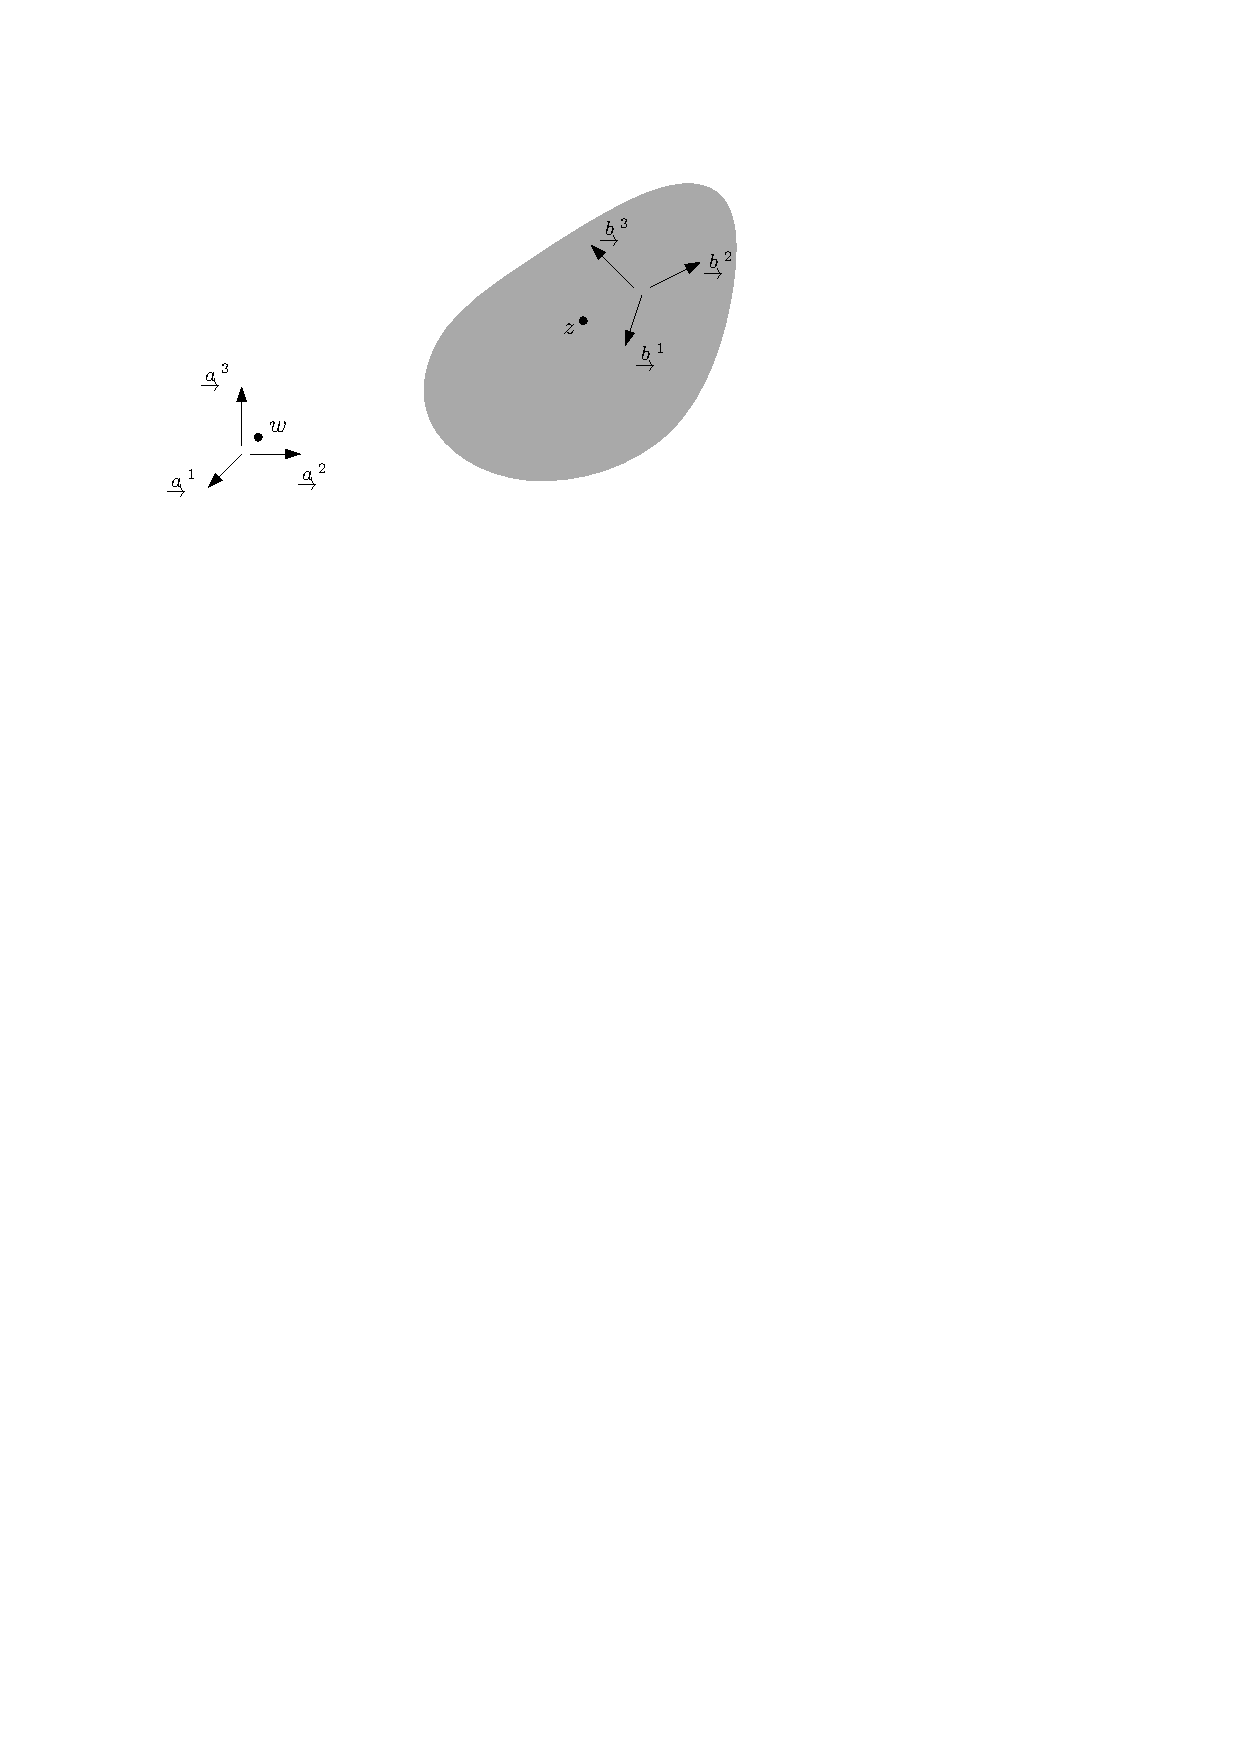
\includegraphics[width=0.7\textwidth]{figs/prob.pdf}
	\caption[Problem setup.]{Problem setup.}
	\label{fig:se3_prob}
\end{figure}
The estimated states are $\mbf{r}_a^{zw}$ and $\mbf{C}_{ab}$. The pose can be represented as an element of $SE(3)$ as
\bdis
	\mbf{T}_{ab} = 
	\bma{cc}
		\mbf{C}_{ab} & \mbf{r}_a^{zw} \\
		\mbf{0} & 1
	\ema.
\edis The kinematics of this problem are
\begin{align*}
	\mbfdot{C}_{ab} &= \mbf{C}_{ab} \mbs{\omega}_b^{{ba}^\times}, \\
	\mbfdot{r}_a^{zw} &= \mbf{v}_a^{zw/a}.
\end{align*}
In matrix form, the kinematics are 
\bdis
	\mbfdot{T}_{ab} = \mbf{T}_{ab}\mbs{\varpi}_b^\wedge,
\edis
where $\mbs{\varpi}_b = \left[ \; {\mbs{\omega}_b^{ba}}^\trans \; {\mbf{v}_b^{zw/a}}^\trans \; \right]^\trans$. 
The body is equipped with a rate gyro which measures
\bdis
	\mbf{u}_b^1 = \mbs{\omega}_b^{ba} - \mbf{w}_b^1,
\edis
where $\mbf{w}_{b}^1$ is band-limited white noise. When discretized, $\mbf{w}_{b_k}^1 \sim \mathcal{N}\left(0,\mbf{Q}_k^1\right)$.  The body is also equipped with a velocity sensor that measures
\bdis
	\mbf{u}_b^2 = \mbf{v}_{b}^{zw/a} - \mbf{w}_b^2,
\edis
where $\mbf{w}_{b}^2$ is band-limited white noise. When discretized, $\mbf{w}_{b_k}^2 \sim \mathcal{N}\left(0,\mbf{Q}_k^2\right)$. Rearranging and substituting into the kinematics leads to
\begin{align*}
	\mbfdot{C}_{ab} &= \mbf{C}_{ab} \left(\mbf{u}_b^1 + \mbf{w}_b^1\right)^\times, \\
	\mbfdot{r}_a^{zw} &= \mbf{C}_{ab} \left(\mbf{u}_b^2 +  \mbf{w}_b^2 \right).
\end{align*}
Incorporating the measurement model, the kinematics in matrix form are 
\bdis
	\mbfdot{T}_{ab} = \mbf{T}_{ab}\left(\mbf{u}_b +  \mbf{w}_b \right)^\wedge,
\edis
where $\mbf{u}_b = \left[ \; {\mbf{u}_b^1}^\trans \; {\mbf{u}_b^2}^\trans \; \right]^\trans$ and $\mbf{w}_b = \left[ \; {\mbf{w}_b^1}^\trans \; {\mbf{w}_b^2}^\trans \; \right]^\trans$. Throughout this chapter, the subscripts on $\mbf{T}_{ab}$ are dropped to be concise.


\subsection{Left-Invariant Extended Kalman Filter Derivation}
\label{ssec:se3_LIEKF}

In order to derive a LIEKF, the exteroceptive measurement model must be left invariant. In this case, approriate measurements are position measurements, which could be from a GPS receiver, for example. The discrete-time measurement model is
\beq
	\bma{c} \mbf{y}_{a_k} \\ 0 \ema = \bma{c} \mbf{r}_a^{z_k w} +  \mbf{v}_{a_k} \\ 1 \ema = \mbf{T}_k
	\bma{c}
		\mbf{0} \\
		1
	\ema
	+ 
	\bma{c}
		\mbf{v}_{a_k} \\
		0
	\ema, \label{eq:se3_meas_left}
\eeq
where $\mbf{v}_{a_k} \sim \mathcal{N}\left(\mbf{0},\mbf{R}_k\right)$. 

The left-invariant error  $\mbfdel{T} = \mbf{T}^{-1}\mbfhat{T}$ is used because the measurement model is left invariant. The error propagation is 
\begin{align} 
	\delta \mbfdot{T} & = \mbfdot{T}^{-1} \mbfhat{T} + \mbf{T}^{-1}\dot{\mbfhat{T}} \nonumber \\
	& = -\mbf{T}^{-1} \mbfdot{T} \mbf{T}^{-1} \mbfhat{T} + \mbf{T}^{-1} \mbfhat{T} \mbf{u}_b^\wedge \nonumber \\
	& = -\mbf{T}^{-1} \mbf{T} \left(\mbf{u}_b + \mbf{w}_b\right)^\wedge \mbf{T}^{-1} \mbfhat{T} + \mbfdel{T} \mbf{u}_b^\wedge \nonumber \\
	& = -\left(\mbf{u}_b + \mbf{w}_b\right)^\wedge  \mbfdel{T} + \mbfdel{T} \mbf{u}_b^\wedge  \label{eq:se3_left_1}.
\end{align}
To linearize \eqref{eq:se3_left_1}, let $\mbfdel{T} \approx \mbf{1} + \mbsdel{\xi}^\wedge$, $\mbfdel{T}^{-1} \approx \mbf{1} - \mbsdel{\xi}^\wedge$,  and $\mbf{w}_b = \mbfdel{w}_b$. Neglecting second order terms, \eqref{eq:se3_left_1} is then approximated as
\begin{align} 
	\f{\dee}{\dt} \left(\mbf{1} + \mbsdel{\xi}^\wedge\right) & = \left(\mbf{1} + \mbsdel{\xi}^\wedge\right) \mbf{u}_b^\wedge -\left(\mbf{u}_b + \mbfdel{w}_b\right)^\wedge \left(\mbf{1} +\mbsdel{\xi}^\wedge\right), \nonumber \\
	\delta \mbsdot{\xi}^\wedge & = \mbf{u}_b^\wedge + \mbsdel{\xi}^\wedge \mbf{u}_b^\wedge - \left(\mbf{u}_b + \mbfdel{w}_b\right)^\wedge - \left(\mbf{u}_b + \mbfdel{w}_b\right)^\wedge \mbsdel{\xi}^\wedge \nonumber \\
	 & = \mbsdel{\xi}^\wedge \mbf{u}_b^\wedge - \mbf{u}_b^\wedge \mbsdel{\xi}^\wedge -\mbfdel{w}_b^\wedge .  \label{eq:se3_left_2}
\end{align}
Using the identity \eqref{eq:ad_identity}, \eqref{eq:se3_left_2} is rewritten as
\bdis
	\delta \mbsdot{\xi}^\wedge = \left(-\textrm{ad}(\mbf{u}_b) \mbsdel{\xi}\right)^\wedge - \mbfdel{w}_b^\wedge,
\edis
which in turn can be written as
\bdis
	\delta \mbsdot{\xi} = -\textrm{ad}(\mbf{u}_b) \mbsdel{\xi} - \mbfdel{w}_b.
\edis
Therefore, $\mbf{A} = -\textrm{ad}(\mbf{u}_b)$ and $\mbf{L} = -\mbf{1}$. Notice that $\mbf{A}$ is only a function of the measurement $\mbf{u}_b$.

When a position measurement $\mbf{y}_{a_k}$ is available, the state estimate is corrected. This correction has the form
\bdis
	\mbfhat{T}_k = \mbfcheck{T}_k\exp\left(-\left(\mbf{K}_k\mbf{z}_k\right)^\wedge\right) .
\edis
The innovation is
\begin{align}
	\bma{c} \mbf{z}_k \\ 0 \ema &= \mbfcheck{T}_k^{-1}\left(\bma{c} \mbf{y}_{a_k} \\ 1 \ema - \bma{c} \mbfcheck{y}_{a_k} \\ 1 \ema\right) \nonumber \\
	&= \mbfcheck{T}_k^{-1} \left(\mbf{T}_k \bma{c} \mbf{0} \\	1 \ema + \bma{c} \mbf{v}_{a_k} \\0 \ema - \mbfch{T}_k \bma{c} \mbf{0} \\ 1 	\ema \right) \nonumber \\
	&= \delta \mbfch{T}_k^{-1} \bma{c} \mbf{0} \\	1 \ema + \mbfch{T}_k^{-1}\bma{c} \mbf{v}_{a_k} \\0 \ema - \bma{c} \mbf{0} \\ 1 \ema. \label{eq:se3_left_3}
\end{align}
Linearizing \eqref{eq:se3_left_3} by letting  $\delta \mbfcheck{T}_k^{-1} \approx \mbf{1} - \delta \mbscheck{\xi}_k^\wedge$ and $\mbf{v}_{a_k} = \mbfdel{v}_{a_k}$,
\begin{align}
	\bma{c} \mbf{z}_k \\ 0 \ema &\approx \left(\mbf{1} - \delta \mbscheck{\xi}_k^\wedge\right) 
\bma{c}
	\mbf{0} \\
	1
\ema +
\mbfcheck{T}_k^{-1}
\bma{c}
	\mbfdel{v}_{a_k} \\
	0
\ema - 	
\bma{c}
	\mbf{0} \\
	1
\ema \nonumber \\
	& = -\delta \mbscheck{\xi}_k^\wedge 
\bma{c}
	\mbf{0} \\
	1
\ema + \mbfcheck{T}_k^{-1}
\bma{c}
	\mbfdel{v}_{a_k} \\
	0
\ema \nonumber \\
	& =  
-\bma{cc}
	{\delta\mbscheck{\xi}^\phi}^\times & \delta\mbscheck{\xi}_k^\textrm{r} \\
 	\mbf{0} & 0 
\ema 
\bma{c}
	\mbf{0} \\
	1
\ema + \mbfcheck{T}_k^{-1}
\bma{c}
	\mbfdel{v}_{a_k} \\
	0
\ema \nonumber \\
	& =  
	\mbftilde{H} \delta \mbscheck{\xi}_k + \mbfcheck{T}_k^{-1}
\bma{c}
	\mbfdel{v}_{a_k} \\
	0
\ema , \label{eq:se3_left_4}
\end{align}
where 
\bdis
	\mbftilde{H} = 
	\bma{cc}
		\mbf{0} & -\mbf{1} \\
		\mbf{0} & \mbf{0}
	\ema.
\edis
Noting that the bottom row of \eqref{eq:se3_left_4} is only zeros, it can be written
\bdis
	\mbf{z}_k = \mbf{H} \delta \mbscheck{\xi}_k + \mbf{M}_k \mbfdel{v}_{a_k}
\edis
where
\bdis
	\mbf{H} = 
	\bma{cc}
		\mbf{0} & -\mbf{1} \\
	\ema
\edis
and $\mbf{M}_k = \mbfch{C}_{ab_k}^\trans$. Notice that $\mbf{H}$ is constant.

\subsection{Right-Invariant Extended Kalman Filter Derivation}
\label{ssec:SE3_RIEKF}

In order to derive a RIEKF, the exteroceptive measurement model must be right invariant. In this case, appropriate measurements are landmark measurements resolved in (i.e. observed in) the body frame, which could be from a LIDAR or camera, for example. In reality, the measurement model depends on the sensor. However, for the sake of simplicity, the exteroceptive measurements are modelled as relative landmark locations. This ensures the measurement model is actually right-invariant. Let point $p^i$ be associated with the $i^{th}$ landmark. The position of the $i^{th}$ landmark relative to point $w$ resolved in $\rframe{a}$ is $\mbf{r}_a^{p_iw}$. The landmark sensor is assumed to measure $\mbf{r}_b^{p_iz}$. Figure~\ref{fig:se3_prob_landmarks} displays the geometry of the problem. 
\begin{figure}
	\centering
	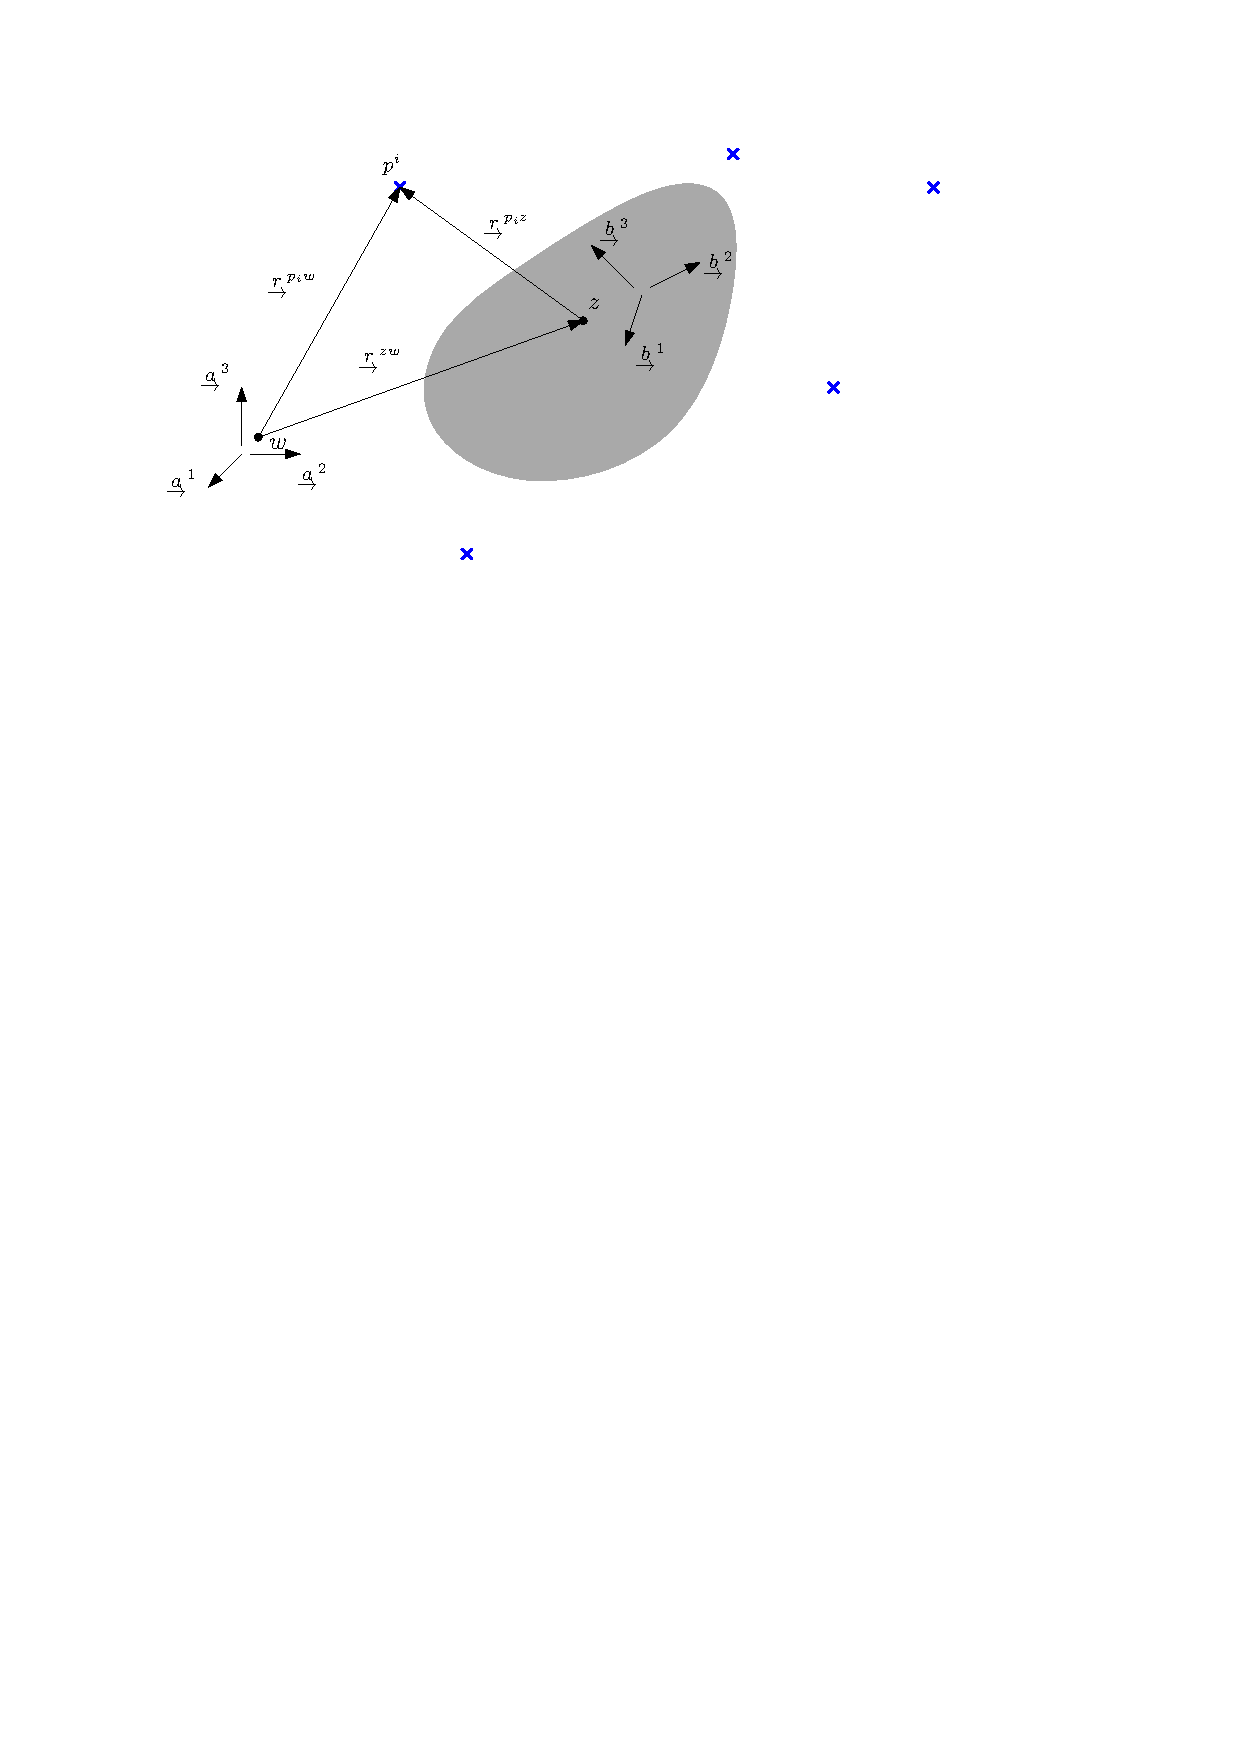
\includegraphics[width=0.7\textwidth]{figs/prob_landmarks.pdf}
	\caption{Problem setup, where the blue crosses are the observed landmarks.}
	\label{fig:se3_prob_landmarks}
\end{figure}
The discrete-time measurement model is then
\beq
	\bma{c} \mbf{y}_{b_k}^i \\ 1 \ema = \bma{c} \mbf{C}_{ab_k}^\trans\left( \mbf{r}_a^{p_iw} - \mbf{r}_a^{z_k w} \right) +  \mbf{v}_{b_k}^i \\ 1 \ema = \mbf{T}_k^{-1}
	\bma{c}
		 \mbf{r}_a^{p_iw}\\
		1
	\ema
	+ 
	\bma{c}
		\mbf{v}_{b_k}^i \\
		0
	\ema, \label{eq:se3_meas_right}
\eeq
where $\mbf{v}_{b_k}^i \sim \mathcal{N}\left(\mbf{0},\mbf{R}_k^i\right)$, $i = 1,\ldots,m$, where $m$ is the number of landmarks.

The right-invariant error  $\mbfdel{T} = \mbfhat{T}\mbf{T}^{-1}$ is used. The error propagation is
\begin{align} 
	\delta \mbfdot{T} & = \dot{\mbfhat{T}}\mbf{T}^{-1}  + \mbfhat{T}\mbfdot{T}^{-1} \nonumber \\
	& = \mbfhat{T} \mbf{u}_b^\wedge\mbf{T}^{-1}   - \mbfhat{T}\mbf{T}^{-1} \mbfdot{T} \mbf{T}^{-1} \nonumber \\
	& = \mbfhat{T} \mbf{u}_b^\wedge\mbf{T}^{-1}  - \mbfhat{T}\mbf{T}^{-1}\mbf{T}\left(\mbf{u}_b + \mbf{w}_b\right)^\wedge \mbf{T}^{-1}  \nonumber \\
	& = \mbfhat{T} \left(\mbf{u}_b - \mbf{u}_b - \mbf{w}_b\right)^\wedge \mbf{T}^{-1}  \nonumber \\
	& = -\mbfhat{T}\mbf{w}_b^\wedge\mbfhat{T}^{-1}\mbfdel{T}  \nonumber \\
	& = -\left(\textrm{Ad}(\mbfhat{T})\mbf{w}_b\right)^\wedge\mbfdel{T}  \label{eq:se3_right_1}.
\end{align}
To linearize \eqref{eq:se3_right_1}, let $\mbfdel{T} \approx \mbf{1} + \mbsdel{\xi}^\wedge$  and $\mbf{w}_b = \mbfdel{w}_b$. Neglecting second order terms, \eqref{eq:se3_right_1} is then 
\begin{align} 
	\f{\dee}{\dt} \left(\mbf{1} + \mbsdel{\xi}^\wedge\right) & = -\left(\textrm{Ad}(\mbfhat{T})\mbfdel{w}_b\right)^\wedge\left(\mbf{1} +\mbsdel{\xi}^\wedge\right), \nonumber \\
	\delta \mbsdot{\xi}^\wedge & = -\left(\textrm{Ad}(\mbfhat{T})\mbfdel{w}_b\right)^\wedge, \nonumber \\
	\delta \mbsdot{\xi} & = -\textrm{Ad}(\mbfhat{T})\mbfdel{w}_b.  \label{eq:se3_right_2}
\end{align}
Therefore, $\mbf{A} = \mbf{0}$ and $\mbf{L} =  -\textrm{Ad}(\mbfhat{T})$. Notice that $\mbf{A}$ is constant.		

\mymargin{Edited 2021/2/17} 
When a relative landmark measurement $\mbf{y}_{b_k}^i$ is available, the state estimate is corrected. This correction has the form
\bdis
	\mbfhat{T}_k =  \exp\left(-\left(\mbf{K}_k\mbf{z}_k\right)^\wedge\right)\mbfcheck{T}_k.
\edis
The innovation associated with the $i^{th}$ landmark is
\begin{align}
	\bma{c} \mbf{z}_k^i \\ 0 \ema &= \mbfcheck{T}_k\left(\bma{c} \mbf{y}_{b_k}^i \\ 1 \ema - \bma{c} \mbfcheck{y}_{b_k}^i \\ 1 \ema\right) \nonumber \\
	&= \mbfcheck{T}_k \left(\mbf{T}_k^{-1} \bma{c} \mbf{r}_a^{p_iw} \\	1 \ema + \bma{c} \mbf{v}_{b_k}^i \\0 \ema - \mbfch{T}_k^{-1} \bma{c} \mbf{r}_a^{p_iw} \\ 1 	\ema \right) \nonumber \\
	&= \delta \mbfch{T}_k \bma{c} \mbf{r}_a^{p_iw} \\	1 \ema + \mbfch{T}_k\bma{c} \mbf{v}_{b_k}^i \\0 \ema - \bma{c} \mbf{r}_a^{p_iw} \\ 1 \ema. \label{eq:se3_right_3}
\end{align}
Linearizing \eqref{eq:se3_right_3} by letting  $\delta \mbfcheck{T}_k \approx \mbf{1} + \delta \mbscheck{\xi}_k^\wedge$ and $\mbf{v}_{b_k} = \mbfdel{v}_{b_k}$,
\begin{align}
	\bma{c} \mbf{z}_k^i \\ 0 \ema &\approx \left(\mbf{1} + \delta \mbscheck{\xi}_k^\wedge\right) 
\bma{c}
	\mbf{r}_a^{p_iw} \\
	1
\ema +
\mbfcheck{T}_k
\bma{c}
	\mbfdel{v}_{b_k}^i \\
	0
\ema - 	
\bma{c}
	\mbf{r}_a^{p_iw} \\
	1
\ema \nonumber \\
	& = \delta \mbscheck{\xi}_k^\wedge 
\bma{c}
	\mbf{r}_a^{p_iw} \\
	1
\ema + \mbfcheck{T}_k
\bma{c}
	\mbfdel{v}_{b_k}^i \\
	0
\ema \nonumber \\
	& =  
\bma{cc}
	{\delta\mbscheck{\xi}_k^{\phi}}^\times & \delta\mbscheck{\xi}_k^\textrm{r} \\
 	\mbf{0} & 0 
\ema 
\bma{c}
	\mbf{r}_a^{p_iw} \\
	1
\ema + \mbfcheck{T}_k
\bma{c}
	\mbfdel{v}_{b_k}^i \\
	0
\ema \nonumber \\
	& =  
\bma{c}
	{\delta\mbscheck{\xi}_k^{\phi}}^\times\mbf{r}_a^{p_iw} + \delta\mbscheck{\xi}_k^\textrm{r} \\
 	\mbf{0} 
\ema 
 + \mbfcheck{T}_k
\bma{c}
	\mbfdel{v}_{b_k}^i \\
	0
\ema \nonumber \\
	& =  
\bma{c}
	-{\mbf{r}_a^{p_iw}}^\times{\delta\mbscheck{\xi}_k^{\phi}} + \delta\mbscheck{\xi}_k^\textrm{r} \\
 	\mbf{0} 
\ema 
 + \mbfcheck{T}_k
\bma{c}
	\mbfdel{v}_{b_k}^i \\
	0
\ema \nonumber \\
	& =  
	\mbf{H}^i \delta \mbscheck{\xi}_k + \mbfcheck{T}_k
\bma{c}
	\mbfdel{v}_{b_k}^i \\
	0
\ema , \label{eq:se3_right_4}
\end{align}
where 
\bdis
	\mbftilde{H} = 
	\bma{cc}
		-{\mbf{r}_a^{p_iw}}^\times & \mbf{1} \\
		\mbf{0} & \mbf{0}
	\ema.
\edis
Noting that the bottom row of \eqref{eq:se3_right_4} is full of zeros, it can be written
\bdis
	\mbf{z}_k^i = \mbf{H}^i \delta \mbscheck{\xi}_k + \mbf{M}_k \mbfdel{v}_{b_k}^i
\edis
where
\bdis
	\mbf{H}^i = 
	\bma{cc}
		-{\mbf{r}_a^{p_iw}}^\times & \mbf{1} \\
	\ema
\edis
and $\mbf{M}_k = \mbfch{C}_{ab_k}^\trans$. For the $m$ landmarks,
\beq
	\mbf{H} = \underset{i = 1,\ldots,m}{\textrm{row}}\left(
	\bma{cc}
		-{\mbf{r}_a^{p_iw}}^\times & \mbf{1} \\
	\ema
	\right) \label{eq:se3_H_riekf}
\eeq
and $\mbf{M}_k = \textrm{diag}\left(\mbfcheck{C}_{ab_k}^\trans,\ldots,\mbfcheck{C}_{ab_k}^\trans\right)$. Once again, notice that $\mbf{H}$ is constant, because $\mbf{r}_a^{p_i w} ,  i = 1,  \ldots , m$ are constant and known a priori.

\subsection{MEKF Solutions}
\label{ssec:se3_EKF}

Throughout this section, the results are compared to that of a standard multiplicative extended Kalman filter (MEKF). A MEKF is a variant of the EKF better suited for attitude estimation. The Jacobians for the MEKF are presented here, but no derivation is given. The errors are defined as $\mbfdel{C} = \mbfbar{C}_{ab}^\trans\mbf{C}_{ab}$ and $\mbfdel{r} = \mbf{r}_a^{zw} - \mbfbar{r}_a^{zw}$. Two different MEKFs must be used for the two different measurement models. The first MEKF, which uses the left-invariant measurements \eqref{eq:se3_meas_left}, is referred to as MEKF-L. The MEKF using the right-invariant measurements \eqref{eq:se3_meas_right} is referred to as MEKF-R. The process model Jacobians for both are
\bdis
	\mbf{A} = 
	\bma{cc}
		-{\mbf{u}_b^1}^\times & \mbf{0} \\
		-\mbfhat{C}_{ab}{\mbf{u}_b^2}^\times & \mbf{0}
	\ema,
	\quad
	\mbf{L} = 
	\bma{cc}
		\mbf{1} & \mbf{0} \\
		\mbf{0} & \mbfhat{C}_{ab}
	\ema.
\edis
Note that $\mbf{A}$ depends on the attitude estimate, which was not the case for the IEKFs. For the MEKF-L, the measurement model Jacobians are
\bdis
	\mbf{H} = 
	\bma{cc}
		\mbf{0} & \mbf{1} \\
	\ema,
	\quad
	\mbf{M} = \mbf{1}.
\edis
For the MEKF-R, the measurement model Jacobians are
\bdis
	\mbf{H}_k^i = 
	\bma{cc}
		 \left(\mbfch{C}_{ab_k}^\trans\left( \mbf{r}_a^{p_iw} - \mbfch{r}_a^{z_k^i w} \right)\right)^\times & -\mbfch{C}_{ab_k}^\trans \\
	\ema,
	\quad
	\mbf{M} = \mbf{1}.
\edis
For the $m$ landmarks,
\beq
	\mbf{H}_k = \underset{i = 1,\ldots,m}{\textrm{row}}\left(
	\bma{cc}
		  \left(\mbfch{C}_{ab_k}^\trans\left( \mbf{r}_a^{p_iw} - \mbfch{r}_a^{z_k^i w} \right)\right)^\times & -\mbfch{C}_{ab_k}^\trans \\
	\ema
	\right) \label{eq:se3_H_ekf}
\eeq
and $\mbf{M} = \mbf{1}$. The MEKF-R's measurement model Jacobian $\mbf{H}_k$ depends on the state estimate, which was not the case for the RIEKF.

\subsection{Simulation Results}

In this section, simulations are performed to compare the four Kalman filters shown in Sections~\ref{ssec:se3_LIEKF}, \ref{ssec:SE3_RIEKF}, and \ref{ssec:se3_EKF}, namely the LIEKF, RIEKF, MEKF-L and MEKF-R. The first question raised in the introduction of this chapter asked whether it was advantageous to use an invariant filter over its standard multiplicative counterpart. The second question concerns the effect of noise on the theoretical convergence properties of the IEKF. The two questions are simultaneously addressed in this section. 

\subsubsection{Simulation Parameters}

In one set of trials, the MEKF-L and LIEKF are compared. In another, the RIEKF and MEKF-R are compared. Certain parameters are kept constant throughout the simulation. The trajectory used is shown in Figure~\ref{fig:se3_traj}. The landmarks used in the RIEKF and MEKF-R are also displayed. It is assumed that, at any given time, all the landmarks are visible. The rate gyro and velocity sensor operate at \SI{100}{\Hz}, while the corrections occur at \SI{10}{\Hz}. The trajectory is parametrized such that $\norm{\mbf{v}_b^{zw/a}}$ is constant at \SI{1}{m/s}. The resulting trajectory takes slightly over \SI{30}{\second} to execute, which is generally enough time for the transients associated with the convergence of the filters to dissipate. The attitude is constrained to have constant roll. To simplify the situation, the sensor noise is assumed isotropic. That is, $\mbf{Q}_k^1 = {\sigma_k^1}^2\mbf{1}$, $\mbf{Q}_k^2 = {\sigma_k^2}^2\mbf{1}$, and $\mbf{R}_k^i = {\sigma_k^\textrm{R}}^2\mbf{1}$. Doing this makes the fact $\mbf{M}_k$ may depend on $\mbfch{C}_{ab_k}$ irrelevant because $\mbf{M}_k^\trans\mbf{R}_k \mbf{M}_k = \mbf{R}_k$ thereby making the computation of the Kalman gain independent of $\mbf{M}_k$. In many applications, the covariance matrices are seen as tuning parameters. Here, no tuning is done. Tuning may greatly effect the results, but in simulation, keeping the theoretical values is more valuable because it demonstrates how the filters behave ``out of the box'' without extensive tuning. 
%  Trajectory
\begin{figure}
 \centering
        \begin{subfigure}[b]{0.495\textwidth}
            \centering
            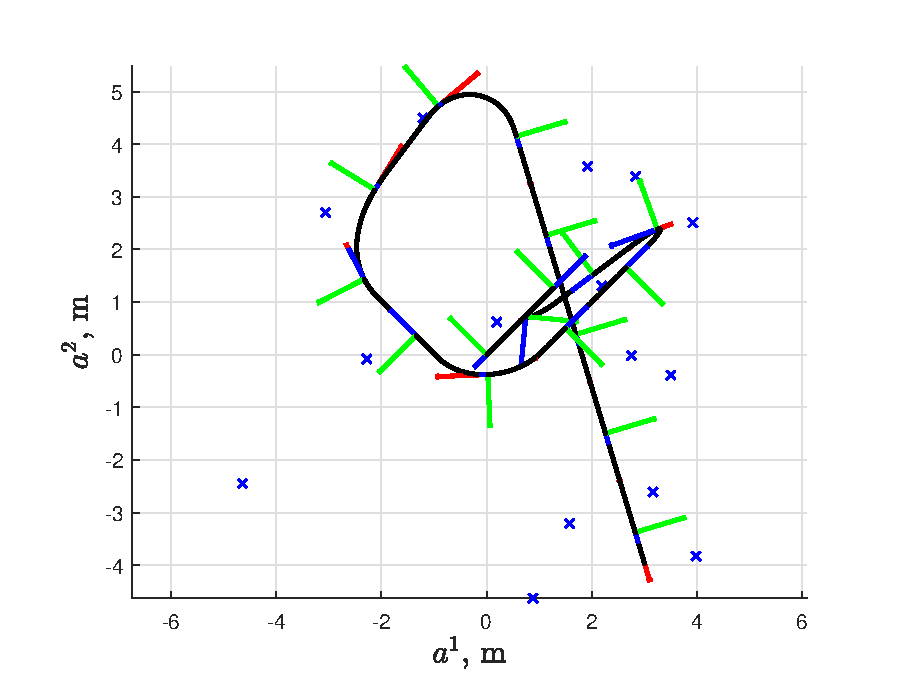
\includegraphics[width=\textwidth]{figs/traj_xy.eps} 
        \end{subfigure}
        \hfill
        \begin{subfigure}[b]{0.495\textwidth}  
            \centering 
            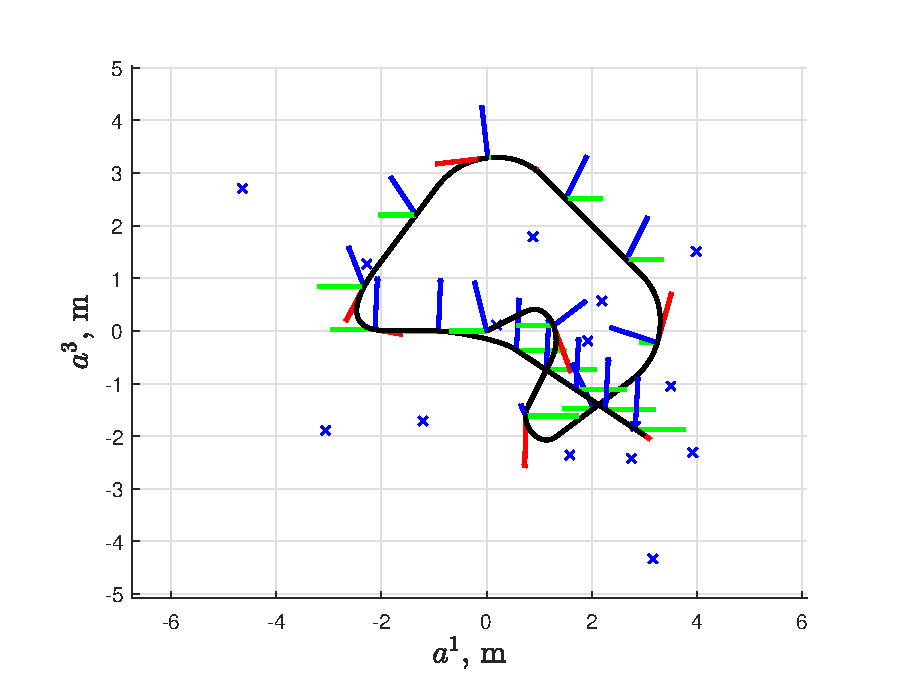
\includegraphics[width=\textwidth]{figs/traj_xz.eps} 
        \end{subfigure}
        \vskip\baselineskip
        \begin{subfigure}[b]{0.495\textwidth}   
            \centering 
            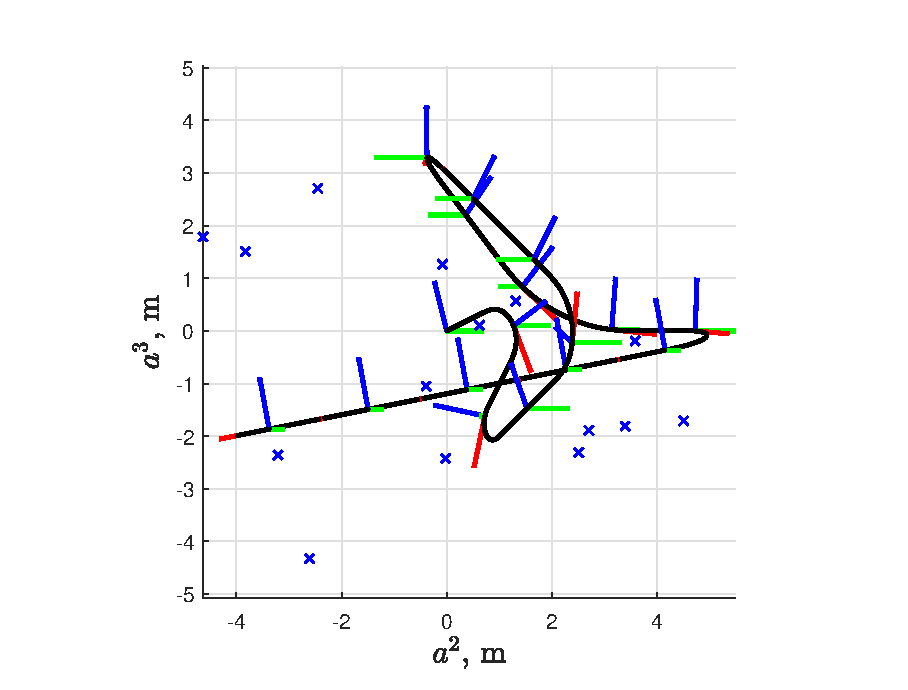
\includegraphics[width=\textwidth]{figs/traj_yz.eps}  
        \end{subfigure}
        \hfill
        \begin{subfigure}[b]{0.495\textwidth}   
            \centering 
            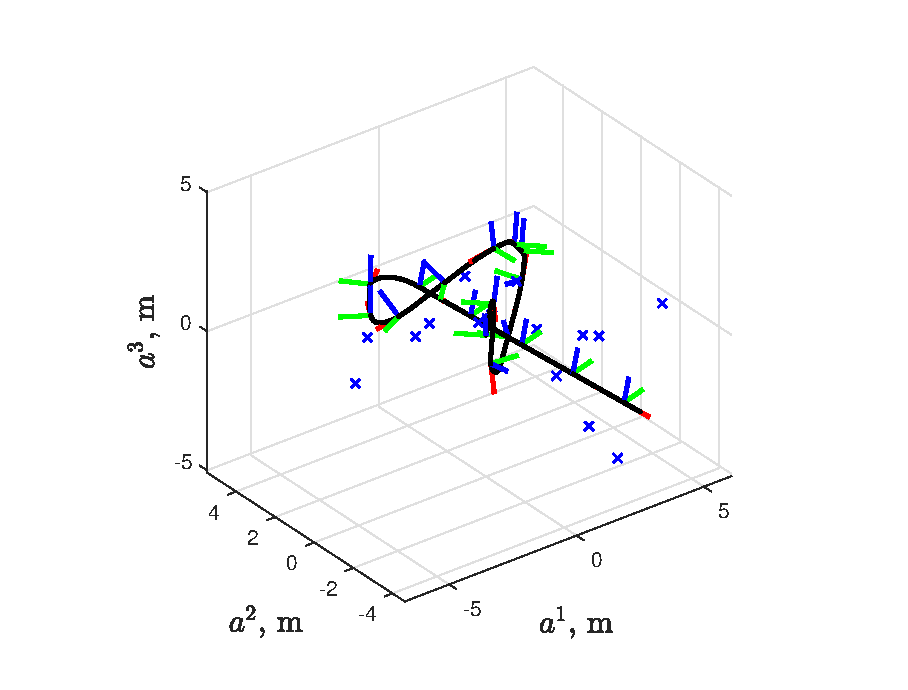
\includegraphics[width=\textwidth]{figs/traj.eps} 
        \end{subfigure} 
	\caption[Trajectory used in simulations.]{Trajectory used in simulations. The blue markers represent the landmarks, the trajectory is shown in black, and a triad is used to show the orientation at various times during the trajectory.}
	\label{fig:se3_traj}
\end{figure}

\subsubsection{Initialization}

To run appropriate Monte Carlo trials, a discussion of the initial error is necessary. When testing any EKF variant using Monte Carlo trials, the initial error $\mbfdel{x}_0$ is drawn from a normal distribution with zero mean and covariance $\mbf{P}_0$. That is, $\mbfdel{x}_0 \sim \mathcal{N}(\mbf{0},\mbf{P}_0)$. This initial error, along with the truth data, is then used to initialize the filters. For the MEKF-R and MEKF-L, this means
\begin{align*}
	\mbfhat{r}_a^{z_0w} &= \mbf{r}_a^{z_0w} - \mbfdel{r}_0, \\
	\mbfhat{C}_{ab_0} &= \mbf{C}_{ab_0}\mbfdel{C}_0^\trans. 
\end{align*}
For the LIEKF, 
\bdis
	\mbfhat{T}_0 = \mbf{T}_0\mbfdel{T}_0,    
\edis
where $\mbfdel{T}_0 = \expmapw{\mbsdel{\xi}_0}$. Similarly, for the RIEKF,
\bdis
	\mbfhat{T}_0 = \mbfdel{T}_0\mbf{T}_0.  
\edis
By using the appropriate error definition to initialize each filter, the same initial error leads to different actual initial conditions. This should not, in theory, change the difficulty of the estimation problem. Nonetheless, the effect of these differing initial conditions is tested. 

To determine the effect of changing the initial error definition, 50 Monte Carlo trials are run using two different ways of initializing the invariant filters. First, the invariant filters are initialized in a manner consistent with their error definition. They are then initialized in the same manner as the MEKF. The sensor noise standard deviations were set to $\sigma_k^1 = \SI{0.05}{rad/s}$, $\sigma_k^2 = \SI{0.05}{m/s}$ and $\sigma_k^\mathrm{R} = \SI{0.05}{\metre}$. The initial errors are drawn from a normal distribution with covariance $\mbf{P}_0 = \mathrm{diag}\left(0.1^2 \mbf{1}, \left(\f{\pi}{4}\right)^2\mbf{1}\right)$, with appropriate units. 

\sloppy The results obtained from initializing the filters in different manners are shown in Table~\ref{tab:se3_mc_err}. In practice, it is preferable to know the error in position and error in attitude separately, rather than the error in the pose. Therefore, it may be more representative to compare the filters using the MEKF error definitions. Thus, unless otherwise specified, the attitude error at each time step is given by	$\delta \phi_k = \log_{SO(3)} \left(\mbfhat{C}_{ab_k}^\trans\mbf{C}_{ab_k} \right)^\vee$ and the position error is $\delta r_k = \norm{\mbf{r}_a^{z_kw} - \mbfhat{r}_a^{z_kw}}$. Using this metric, the initialization technique does not have a significant effect on the performance of the filters. For the LIEKF, changing from the correct initialization to the MEKF initialization sees a slight increase in mean root mean square error (RMSE) for both position and attitude. The difference for the RIEKF is negligible. Importantly, independent of the way the invariant filters are initialized, they still outperform the MEKFs. In this thesis, the appropriate error definition is used to initialize the filters. In fact, doing so ensures that the initial covariance is actually representative of the initial uncertainty in the state estimate, meaning the filters are always consistent to begin the simulation.
\begin{table}[]
\centering
\begin{tabular}{|l|l|l|}
\hline
Filter             & Mean Attitude RMSE (\si{rad}) & Mean Position RMSE (\si{m}) \\ \hhline{|=|=|=|}
MEKF-L             & 0.2035             & 0.0310             \\ \hline
LIEKF - App. Init. & 0.1993             & 0.0288             \\ \hline
LIEKF - MEKF Init. & 0.2017             & 0.0297             \\ \hline
MEKF-R             & 0.0739             & 0.0532             \\ \hline
RIEKF - App. Init. & 0.0734             & 0.0475             \\ \hline
RIEKF - MEKF Init. & 0.0733             & 0.0473             \\ \hline
\end{tabular}
\caption[Results comparing different Monte Carlo initialization methods.]{Mean RMSE in the estimated states over 50 Monte Carlo simulations. The LIEKF and RIEKF were initialized both using an appropriate error definition consistent with the left and right-invariant erros and the error definition used to initialize the MEKFs.}
\label{tab:se3_mc_err}
\end{table}

\subsubsection{Monte Carlo Results}

Having determined the appropriate procedure for comparing the filters, they can be extensively tested to determine the effect of sensor noise on their performance. To do so, the noise in each sensor is varied independently. Four different trials are run. The standard deviations of the noises injected into each measurement for each trial are summarized in Table~\ref{tab:se3_noises}. When the sensor noise is varied, it is incremented by 0.05. At each noise level, 50 Monte Carlo trials are run, where the initial state estimate error and the noise profile is varied.  As in the previous simulations, the initial errors are drawn from a normal distribution with covariance $\mbf{P}_0 = \mathrm{diag}\left(0.1^2 \mbf{1}, \left(\f{\pi}{4}\right)^2\mbf{1}\right)$, with appropriate units. 

\begin{table}[]
\centering
\begin{tabular}{|l|l|l|l|}
\hline
Trial                                            & $\sigma_k^1$ (rad/s)          & $\sigma_k^2$ (m/s)            & $\sigma_k^\textrm{R}$ (m)      \\ \hhline{|=|=|=|=|}
\multicolumn{1}{|l|}{Rate Gyro Noise}            & \multicolumn{1}{l|}{0 to 1} & \multicolumn{1}{l|}{0.05}     & \multicolumn{1}{l|}{0.05}      \\ \hline
\multicolumn{1}{|l|}{Velocity Sensor Noise}      & \multicolumn{1}{l|}{0.05}     & \multicolumn{1}{l|}{0 to 1} & \multicolumn{1}{l|}{0.05}      \\ \hline
\multicolumn{1}{|l|}{Exteroceptive Sensor Noise} & \multicolumn{1}{l|}{0.05}     & \multicolumn{1}{l|}{0.05}     & \multicolumn{1}{l|}{0 to 1} \\ \hline
\multicolumn{1}{|l|}{All Noises}                 & \multicolumn{1}{l|}{0 to 1} & \multicolumn{1}{l|}{0 to 1} & \multicolumn{1}{l|}{0 to 1}  \\ \hline
\end{tabular}
\caption{Standard deviation of the noise injected into each measurement for each trial.}
\label{tab:se3_noises}
\end{table}

The results from varying the noise in the gyro, velocity sensor, correcting sensor, and all the sensors simultaneously can be found in Figures~\ref{fig:comp_noise_gyro_L}~to~\ref{fig:comp_noise_all_R}. 
Each figure presents the mean RMSE at each noise level for the IEKF and MEKF. The shaded areas encompass 80\% of the data, to show the spread of the results. The difference between the mean MEKF and IEKF RMSE is also shown. A positive value indicates that the IEKF outperformed the MEKF. The shaded area once again represents 80\% of the data. A convincing result would see the shaded area be entirely positive, meaning that only on rare occasions did the MEKF outperform the IEKF. 
On average, the invariant filters outperformed the standard MEKF in all the trials. A few important trends to note are as follows.
\begin{itemize}
	\item The increased noise magnitude had a relatively small impact on the MEKF-R and RIEKF, meaning the difference in the filters remained somewhat constant over the all the trials.
	\item Increasing the noise in the velocity sensor led to erratic behaviour of the MEKF-L, leading to some outliers.
	\item Increasing the noise in the GPS measurements led to an increase in the difference between the LIEKF and MEKF-L, as seen in Figure~\ref{fig:comp_noise_corr_L}.
\end{itemize}
It is unsurprising that the IEKF would outperform the MEKF. The state-independent Jacobians mean the computed Kalman gain is accurate, as all the matrices used in its computations are known or are made up of noise-corrupted measurements, except for the error covariance $\mbf{P}$. However, at steady state, the state estimate should be close enough to the true state that the state-dependence of the Jacobians is mitigated. This means that the improvement of the IEKF over the MEKF may simply be due to better performance in the transient. This is investigated in the next section.

%The LIEKF process model Jacobian $\mbf{A}$ depends on the velocity and rate gyro measurements. The MEKF-L process model Jacobian $\mbf{A}$ also depends on the measurement,but also on the attitude estimate $\mbfhat{C}_{ab}$. Their measurement model Jacobian $\mbf{H}$ is identical, and independent of the state. Therefore, if there is any advantage in using the LIEKF, it should manifest itself in a scenario where the attitude estimate is poor and the noise in the interoceptive sensors is low. 
%
%The RIEKF process model Jacobian $\mbf{A}$ is $\mbf{0}$, while the MEKF-R process model Jacobian $\mbf{A}$ depends on both the attitude estimate and the interoceptive measurements. This trend is continued in the measurement model Jacobians. The measurement model Jacobian for the RIEKF depends only on the known landmark position, while it depends on the state estimate for the MEKF-R. The only state dependent Jacobian in the RIEKF is $\mbf{L}$. However, the effect of this state dependency could be dampened by tuning the $\mbf{Q}_k$ matrix. 

\begin{figure}
	\centering
	\begin{subfigure}[b]{0.5\textwidth}
		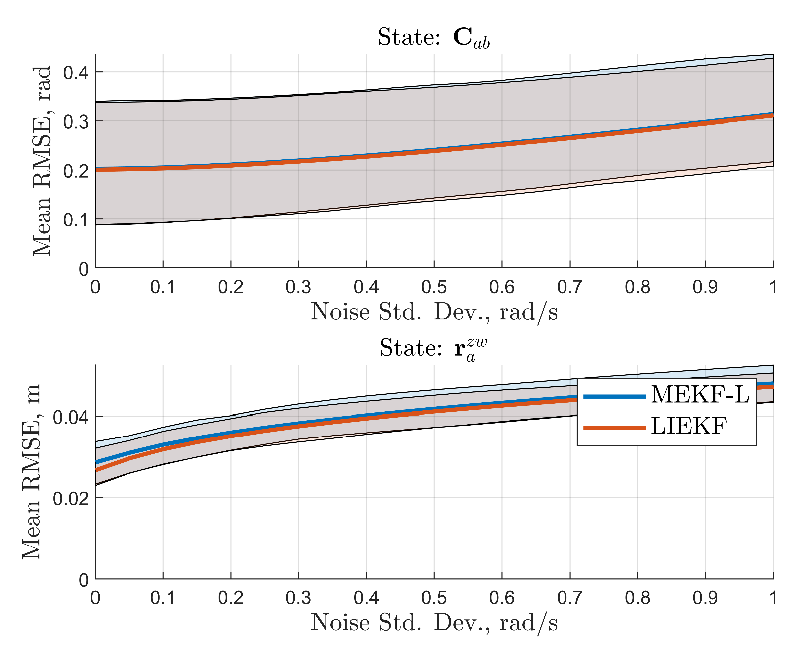
\includegraphics[width=\textwidth]{figs/se3/noise_trials/comp_noise_rmse_state_Gyro_L.eps}
		\caption{Mean RMSE for each state.}
		\label{fig:comp_noise_gyro_L_rmse}
	\end{subfigure}
	~
	\begin{subfigure}[b]{0.5\textwidth}
		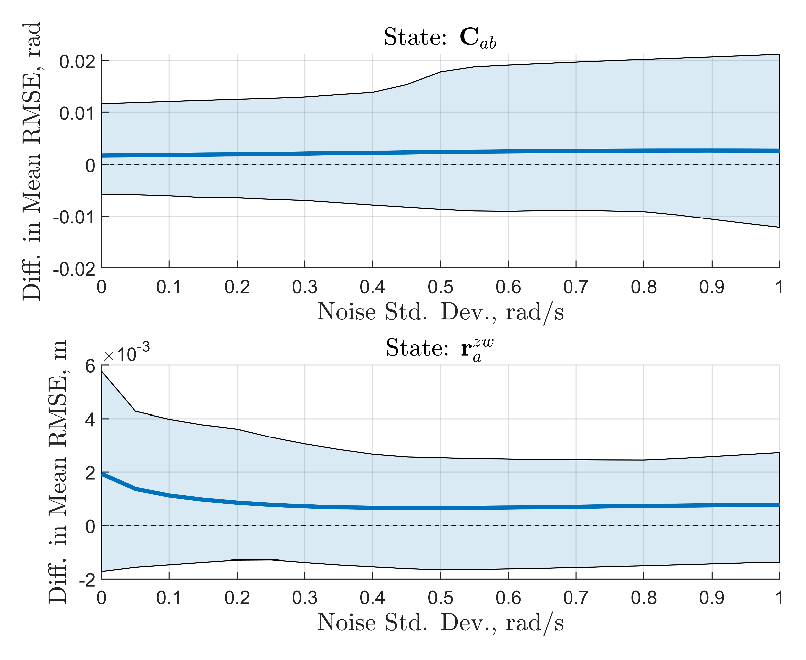
\includegraphics[width=\textwidth]{figs/se3/noise_trials/comp_noise_diff_state_Gyro_L.eps}
		\caption{Difference between in RMSE of MEKF-L and LIEKF.}
		\label{fig:comp_noise_gyro_L_diff}
	\end{subfigure}
	\caption[Results comparing the MEKF-L and LIEKF varying rate gyro noise.]{Results of 50 Monte Carlo simulations comparing the MEKF-L and LIEKF, where the amplitude of the noise in the rate gyro sensor was varied. }
	\label{fig:comp_noise_gyro_L}
\end{figure}

\begin{figure}
	\centering
	\begin{subfigure}[b]{0.5\textwidth}
		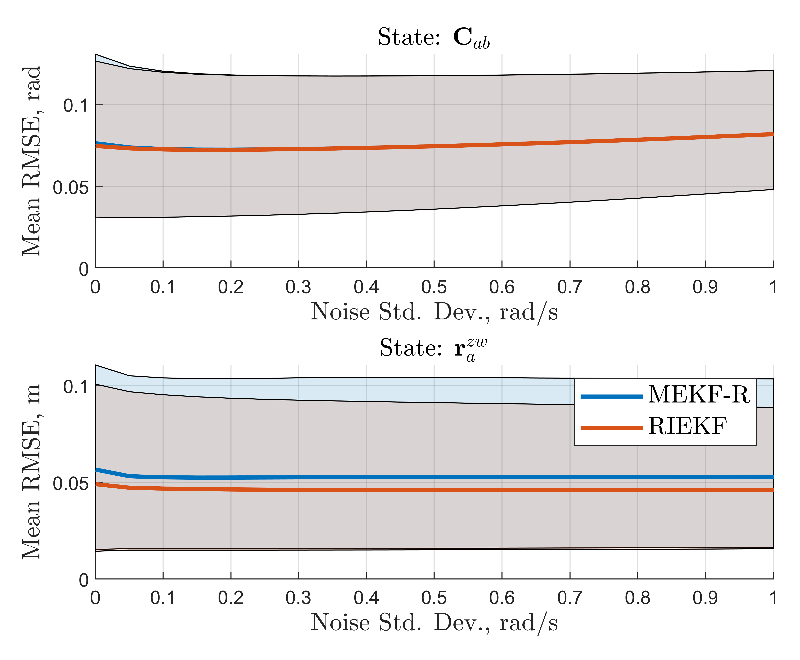
\includegraphics[width=\textwidth]{figs/se3/noise_trials/comp_noise_rmse_state_Gyro_R.eps}
		\caption{Mean RMSE for each state. }
		\label{fig:comp_noise_gyro_R_rmse}
	\end{subfigure}
	~
	\begin{subfigure}[b]{0.5\textwidth}
		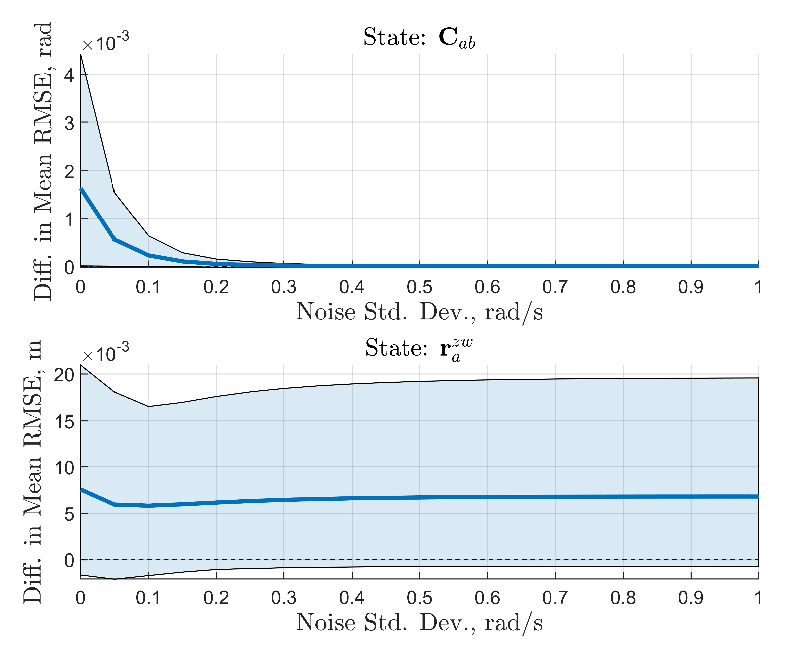
\includegraphics[width=\textwidth]{figs/se3/noise_trials/comp_noise_diff_state_Gyro_R.eps}
		\caption{Difference in RMSE between MEKF-R and RIEKF.}
		\label{fig:comp_noise_gyro_R_diff}
	\end{subfigure}
	\caption[Results comparing the MEKF-R and RIEKF varying rate gyro noise.]{Results of 50 Monte Carlo simulations comparing the MEKF-R and RIEKF, where the amplitude of the noise in the rate gyro sensor was varied. }
	\label{fig:comp_noise_gyro_R}
\end{figure}
% Velocity
\begin{figure}
	\centering
	\begin{subfigure}[b]{0.5\textwidth}
		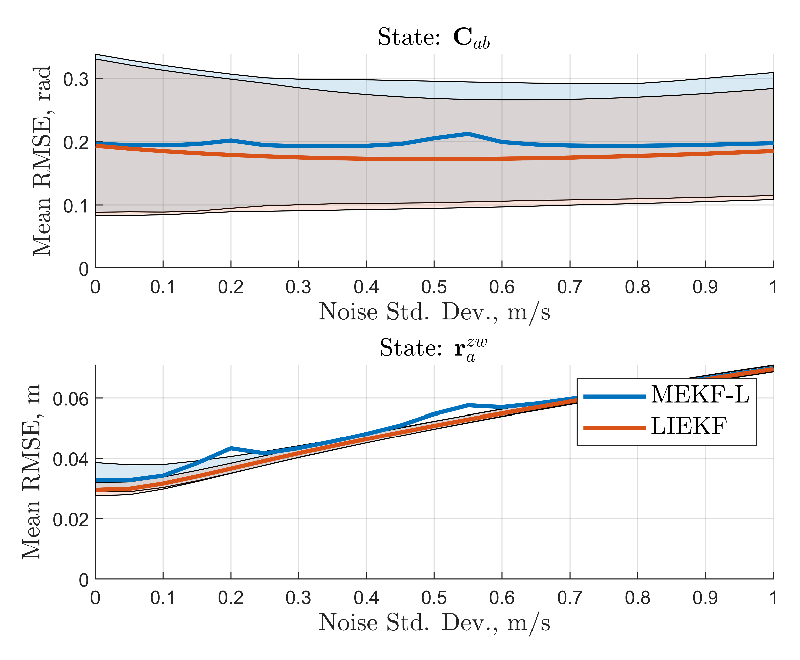
\includegraphics[width=\textwidth]{figs/se3/noise_trials/comp_noise_rmse_state_Vel_L.eps}
		\caption{Mean RMSE for each state.}
	\end{subfigure}
	~
	\begin{subfigure}[b]{0.5\textwidth}
		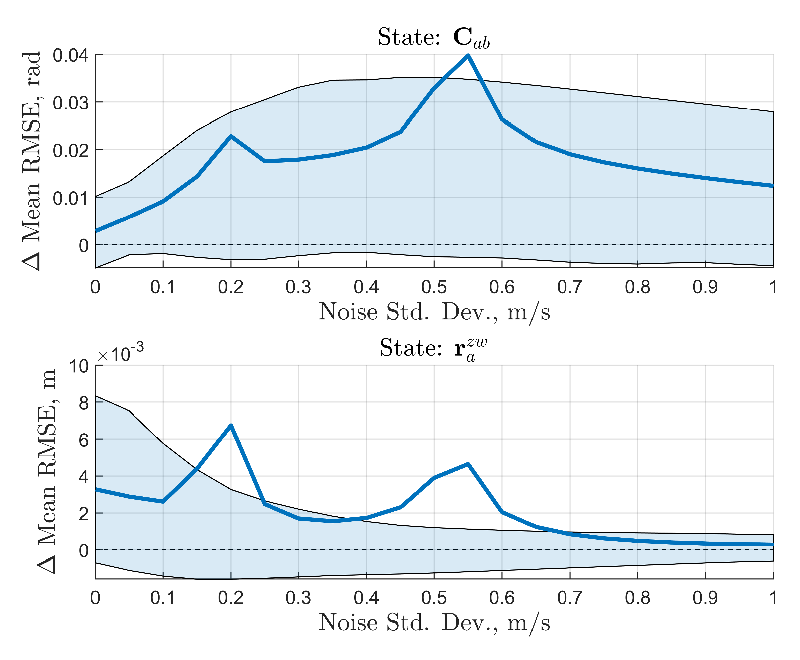
\includegraphics[width=\textwidth]{figs/se3/noise_trials/comp_noise_diff_state_Vel_L.eps}
		\caption{Difference between in RMSE of MEKF-L and LIEKF.}
	\end{subfigure}
	\caption[Results comparing the MEKF-L and LIEKF varying velocity sensor noise.]{Results of 50 Monte Carlo simulations comparing the MEKF-L and LIEKF, where the amplitude of the noise in the velocity sensor was varied. }
	\label{fig:comp_noise_vel_L}
\end{figure}


\begin{figure}
	\centering
	\begin{subfigure}[b]{0.5\textwidth}
		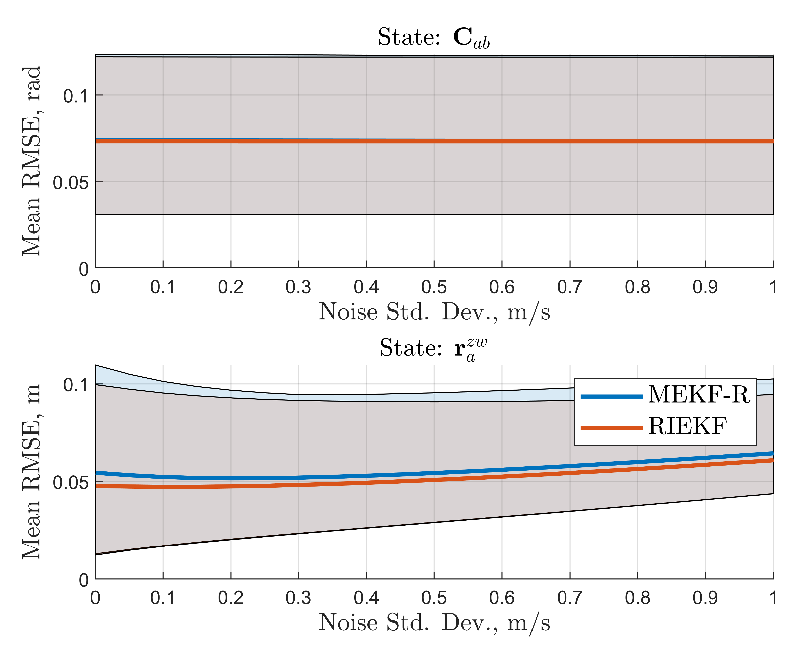
\includegraphics[width=\textwidth]{figs/se3/noise_trials/comp_noise_rmse_state_Vel_R.eps}
		\caption{Mean RMSE for each state.}
	\end{subfigure}
	~
	\begin{subfigure}[b]{0.5\textwidth}
		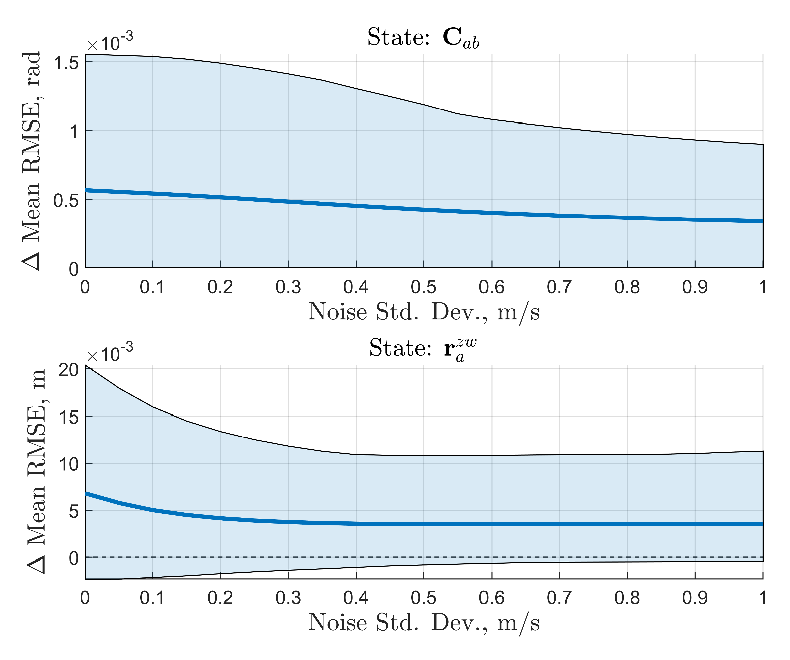
\includegraphics[width=\textwidth]{figs/se3/noise_trials/comp_noise_diff_state_Vel_R.eps}
		\caption{Difference between in RMSE of MEKF-R and RIEKF.}
	\end{subfigure}
	\caption[Results comparing the MEKF-R and RIEKF varying velocity sensor noise.]{Results of 50 Monte Carlo simulations comparing the MEKF-R and RIEKF, where the amplitude of the noise in the velocity sensor was varied. }
	\label{fig:comp_noise_vel_R}
\end{figure}

\begin{figure}
	\centering
	\begin{subfigure}[b]{0.5\textwidth}
		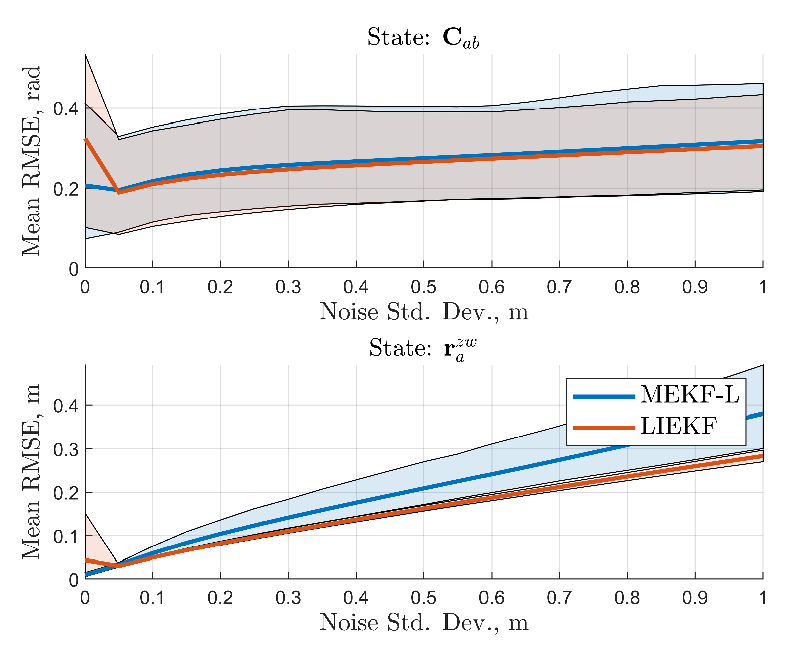
\includegraphics[width=\textwidth]{figs/se3/noise_trials/comp_noise_rmse_state_Corr_L.eps}
		\caption{Mean RMSE for each state.}
	\end{subfigure}
	~
	\begin{subfigure}[b]{0.5\textwidth}
		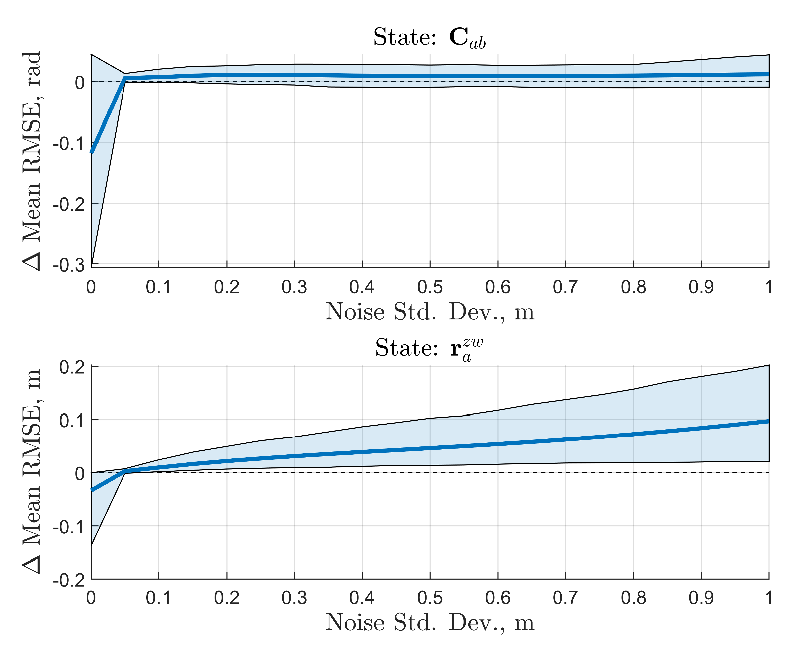
\includegraphics[width=\textwidth]{figs/se3/noise_trials/comp_noise_diff_state_Corr_L.eps}
		\caption{Difference in mean RMSE of MEKF-L and LIEKF.}
	\end{subfigure}
	\caption[Results comparing the MEKF-L and LIEKF varying correcting sensor noise.]{Results of 50 Monte Carlo simulations comparing the MEKF-L and LIEKF, where the amplitude of the noise in the correcting sensor was varied. }
	\label{fig:comp_noise_corr_L}
\end{figure}


\begin{figure}
	\centering
	\begin{subfigure}[b]{0.5\textwidth}
		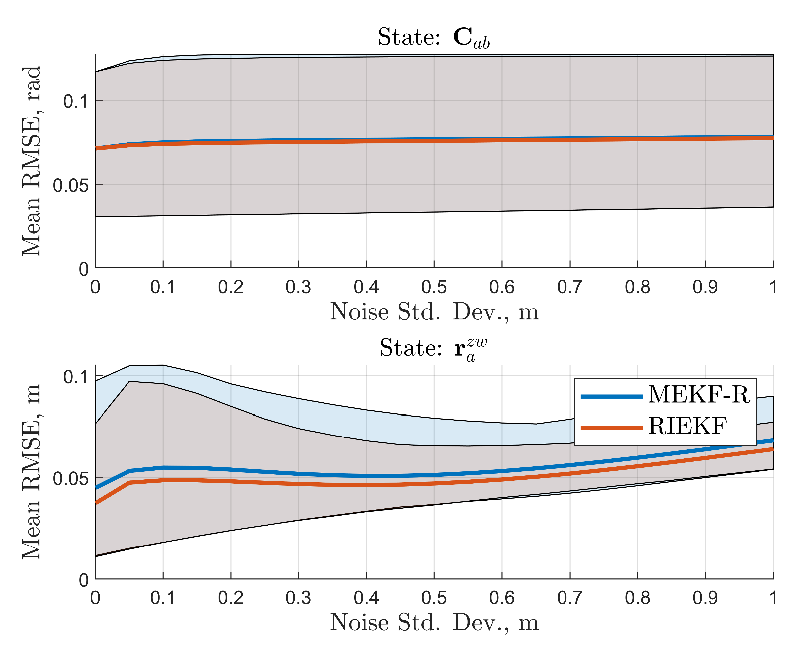
\includegraphics[width=\textwidth]{figs/se3/noise_trials/comp_noise_rmse_state_Corr_R.eps}
		\caption{Mean RMSE for each state.}
	\end{subfigure}
	~
	\begin{subfigure}[b]{0.5\textwidth}
		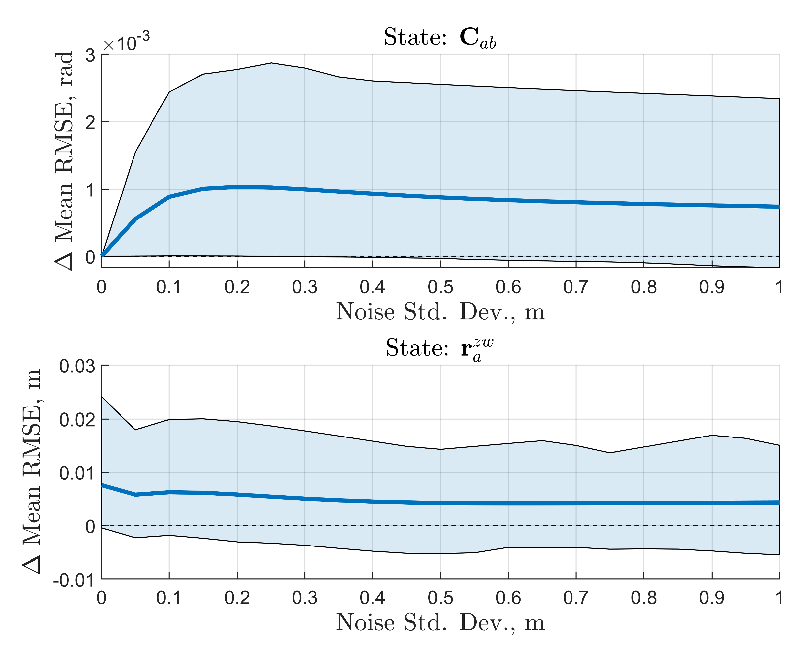
\includegraphics[width=\textwidth]{figs/se3/noise_trials/comp_noise_diff_state_Corr_R.eps}
		\caption{Difference in mean RMSE of MEKF-R and RIEKF.}
	\end{subfigure}
	\caption[Results comparing the MEKF-R and RIEKF varying correcting sensor noise.]{Results of 50 Monte Carlo simulations comparing the MEKF-R and RIEKF, where the amplitude of the noise in the correcting sensor was varied. }
	\label{fig:comp_noise_corr_R}
\end{figure}

% All
\begin{figure}
	\centering
	\begin{subfigure}[b]{0.5\textwidth}
		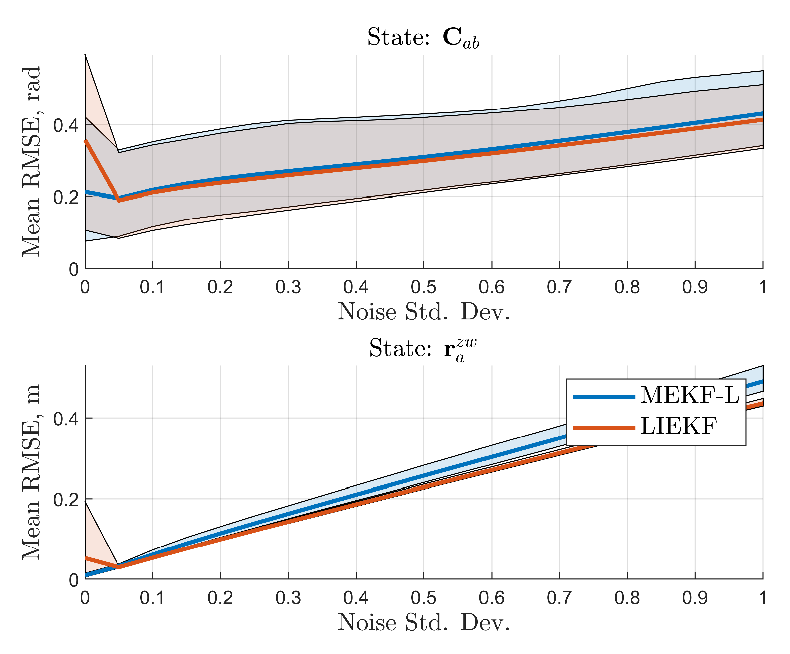
\includegraphics[width=\textwidth]{figs/se3/noise_trials/comp_noise_rmse_state_All_L.eps}
		\caption{Mean RMSE for each state.}
	\end{subfigure}
	~
	\begin{subfigure}[b]{0.5\textwidth}
		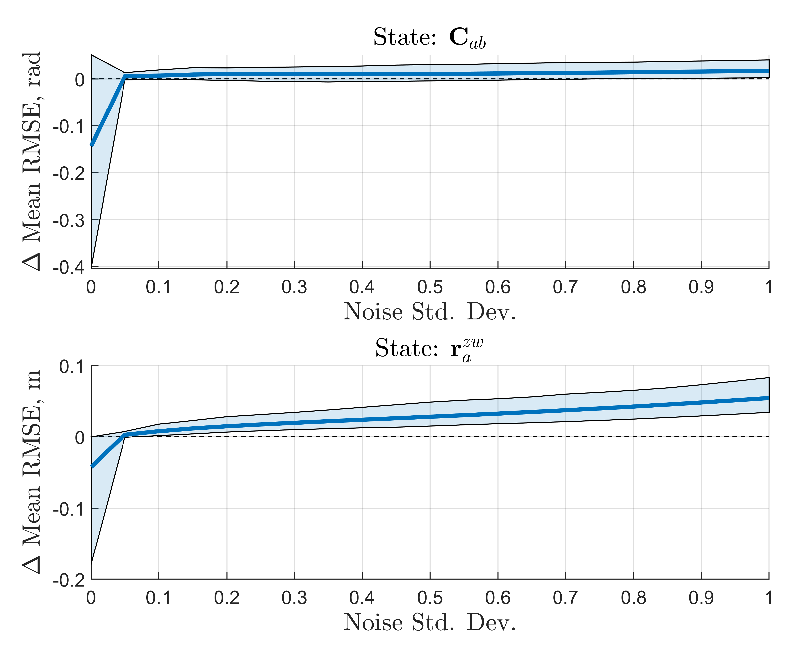
\includegraphics[width=\textwidth]{figs/se3/noise_trials/comp_noise_diff_state_All_L.eps}
		\caption{Difference in mean RMSE of MEKF-L and LIEKF.}
	\end{subfigure}
	\caption[Results comparing the MEKF-L and LIEKF varying all sensor noise.]{Results of 50 Monte Carlo simulations comparing the MEKF-L and LIEKF, where the amplitude of the noise in all sensors was varied. }
	\label{fig:comp_noise_all_L}
\end{figure}

\begin{figure}
	\centering
	\begin{subfigure}[b]{0.5\textwidth}
		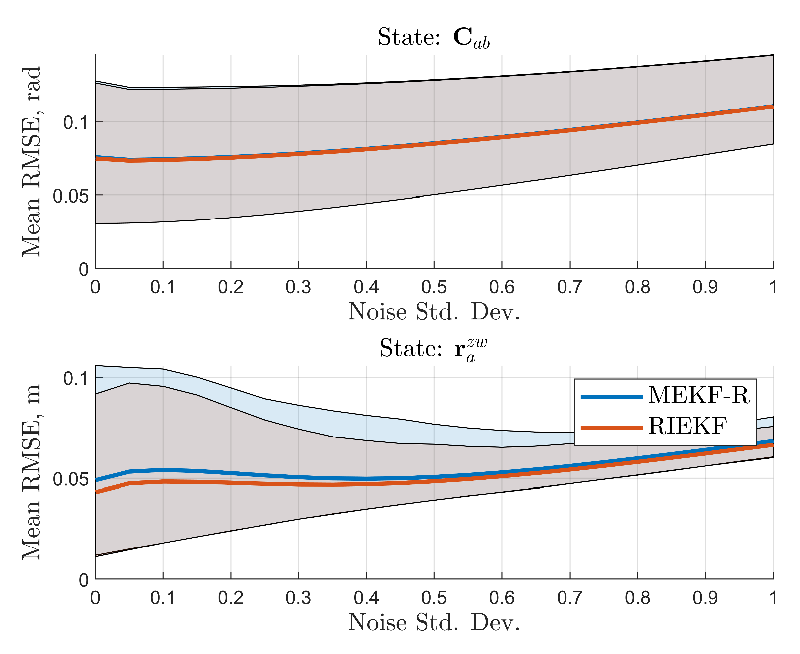
\includegraphics[width=\textwidth]{figs/se3/noise_trials/comp_noise_rmse_state_All_R.eps}
		\caption{Mean RMSE for each state.}
	\end{subfigure}
	~
	\begin{subfigure}[b]{0.5\textwidth}
		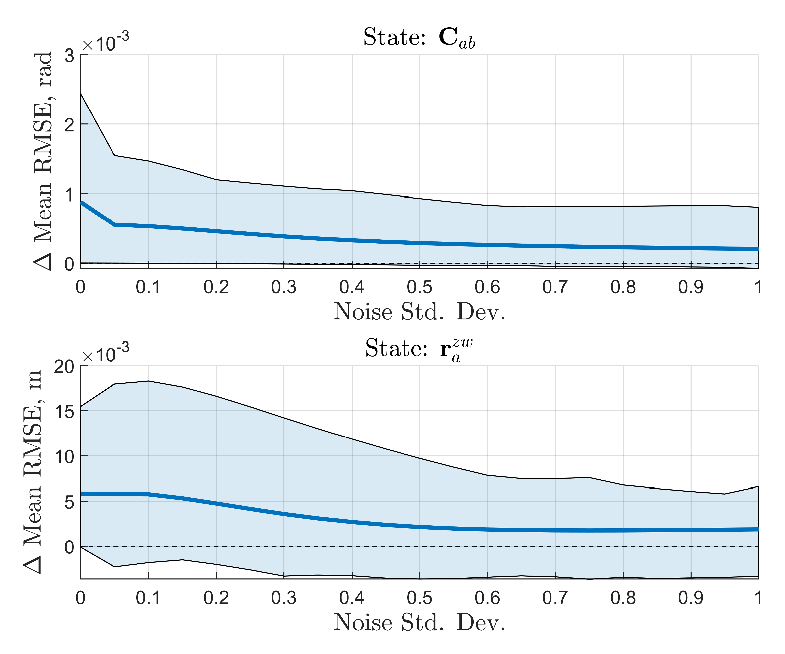
\includegraphics[width=\textwidth]{figs/se3/noise_trials/comp_noise_diff_state_All_R.eps}
		\caption{Difference in mean RMSE of MEKF-R and RIEKF.}
	\end{subfigure}
	\caption[Results comparing the MEKF-R and RIEKF varying all sensor noise.]{Results of 50 Monte Carlo simulations comparing the MEKF-R and RIEKF, where the amplitude of the noise in all sensors was varied. }
	\label{fig:comp_noise_all_R}
\end{figure}

\FloatBarrier

\subsubsection{Effect of Initial Attitude Error}

As discussed in \cite{Barrau2017} and \cite{Barrau2018}, the main advantage the IEKF claims over the MEKF are its convergence properties. Therefore, it may be reasonable to expect the IEKFs to perform substantially better than the MEKFs for high initial error. To test this, $\delta \phi_3$ was varied from 0 \si{\radian} to $\f{23\pi}{24}$ \si{\radian} in increments of \SI{\pi/24}{\radian}. In degrees, $\delta \phi_3$ is varied from  \SI{0}{\degree} to \SI{172.5}{\degree} in increments of \SI{7.5}{\degree}. The initial position was initialized such that there was zero initial error. 

The magnitude of the standard deviation of the noise in the sensors are set to $\sigma_k^1 = \SI{0.05}{rad/s}$, $\sigma_k^2 = \SI{0.05}{m/s}$ and $\sigma_k^\mathrm{R} = \SI{0.05}{m}$. The initial covariance is set $\mbf{P}_0 = \mathrm{diag}(\delta \phi_3^2\mbf{1},1 \times 10^{-4}\mbf{1})$, with appropriate units. This was chosen to reflect the varying uncertainty in the initial attitude and high certainty in the initial position. At each initial attitude error, 50 trials were run, where the noise profile was varied. The results of these simulations are shown in Figure~\ref{fig:comp_att}. The results comparing the RIEKF and MEKF-R show that at high initial attitude, error, the RIEKF consistently outperforms the MEKF-R. This is especially the case for position. The improvement in attitude error is marginal. The trend is less clear when comparing the LIEKF and MEFK-L, but the conclusion is similar. As expected, when the initial estimate of the state is poor, the invariant filters offer superior performance.  When the initial state estimate is accurate, the Jacobians are close to the true Jacobians, nullifying any advantage the IEKFs had over the MEKFs, and their performance is indistinguishable.
\begin{figure}
	\centering
	\begin{subfigure}[b]{0.5\textwidth}
		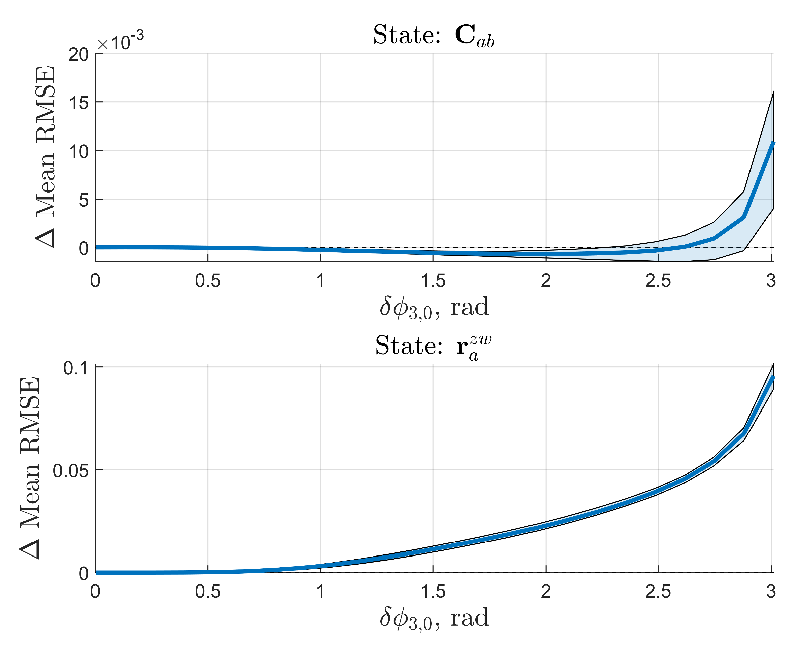
\includegraphics[width=\textwidth]{figs/se3/noise_trials/comp_att_diff_state_Att_R.eps}
		\caption{MEKF-R and RIEKF Comparison.}
	\end{subfigure}
	~
	\begin{subfigure}[b]{0.5\textwidth}
		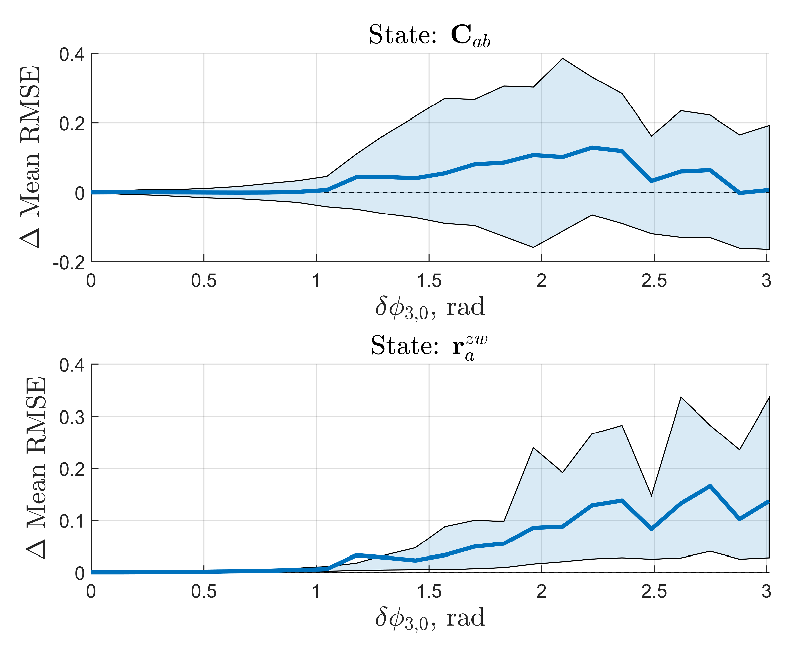
\includegraphics[width=\textwidth]{figs/se3/noise_trials/comp_att_diff_state_Att_L.eps}
		\caption{MEKF-L and LIEKF Comparison.}
	\end{subfigure}
	\caption[Results of different noise profiles where $\delta \phi_3$ was varied.]{Results of 50 different noise profiles comparing invariant and multiplicative filters, where $\delta \phi_3$ was varied. }
	\label{fig:comp_att}
\end{figure}

\FloatBarrier

\section{Applying the IEKF to a Realistic Data Set}
\label{sec:se3_real_data}

The measurement model used in Section~\ref{ssec:SE3_RIEKF} is perfectly right-invariant. However, this is not a realistic measurement model, as no sensor exists that directly measures a relative landmark position. Rather, a LIDAR or camera is used. These measurements are neither left nor right-invariant. Therefore, the IEKF can not be directly applied, and must be adapted, as demonstrated in \cite{Barrau2015aa} with a range-and-bearing measurement model. To illustrate this, the sample problem from the previous section is replicated using a camera as an exteroceptive sensor. Let point $c$ be fixed to the camera, and frame $\rframe{c}$ rotate with the camera. The position of the $i^{th}$ landmark $p^i$ relative to $c$ resolved in the camera frame is 
\beq
	\mbf{r}_{c}^{p_ic} = \mbf{C}_{bc}^\trans(\mbf{C}_{ab}^\trans(\mbf{r}_a^{p_iw} - \mbf{r}_a^{zw}) - \mbf{r}_b^{cz}), \label{eq:se3_real_meas_1}
\eeq
where $\mbf{C}_{bc}$ and $\mbf{r}_b^{cz}$ are known. Letting $\mbf{r}_c^{p_ic} = [ \; x^i \; y^i \; z^i \; ]^\trans$, the measurements from a stereo camera at time $t_k$ are then \cite[p. 208]{Barfoot2017}
\beq
	\mbf{y}_k^i = \mbf{g}(\mbf{r}_{c_k}^{p_ic_k}) =  \f{1}{z_k^i}
	\bma{c}
		f_u x_k^i \\
		f_v y_k^i \\ 
		f_u (x_k^i - b) \\
		f_v y_k^i
	\ema
	+
	\bma{c}
		c_u \\
		c_v \\ 
		c_u \\
		c_v 
	\ema + \mbf{v}_k\label{eq:se3_real_meas}
\eeq
where $c_u$ and $c_v$ are the horizontal and vertical optical centres of the camera in pixels, $f_u$ and $f_v$ are the horizontal and vertical focal lengths of the camera in pixels, and $b$ is the distance between the two centers of projection of the camera, in meters. The noise $\mbf{v}_k \sim \mc{N}(\mbf{0},\mbf{R}_k)$ is zero-mean white noise with covariance $\mbf{R}_k$. 

\subsection{Right-Invariant Kalman Filter Derivation}

As the measurement model \eqref{eq:se3_real_meas} is a function of a right-invariant measurement \eqref{eq:se3_real_meas_1}, a RIEKF is implemented. Therefore, the process model Jacobians from Section~\ref{ssec:SE3_RIEKF} are kept. Typically, the innovation $\mbf{z}_k^i = \mbfch{T}_k(\mbf{y}_k^i - \mbfch{y}_k^i)$ would be linearized to obtain the measurement model Jacobians. However, this is impossible to do in this case, as it is impossible to multiply the measurement from the camera by an element of $SE(3)$.  To avoid this, the standard innovation from the EKF, $\mbf{z}_k^i = \mbf{y}_k^i - \mbfch{y}_k^i$, must be used. 

To compute the new measurement model Jacobians, consider the first-order Taylor series expansion of \eqref{eq:se3_real_meas},
\bdis
	\mbfch{y}_k^i + \mbfdel{y}_k^i =  \mbf{g}(\mbfch{r}_{c_k}^{p_ic_k}) + \underbrace{\left.\f{\partial \mbf{g}(\mbf{r}_{c_k}^{p_ic_k})}{\partial \mbf{x}_k}\right\rvert_{\mbfch{x}_k,\mbfch{v}_k}}_{\mbf{H}_k}\mbfdel{x}_k + \underbrace{\left.\f{\partial \mbf{g}(\mbf{r}_{c_k}^{p_ic_k})}{\partial \mbf{v}_k}\right\rvert_{\mbfch{x}_k,\mbfch{v}_k}}_{\mbf{M}_k}\mbfdel{v}_k.
\edis
Using the chain rule, the matrix $\mbf{H}_k$ is
\bdis
	\mbf{H}_k = \left.\f{\partial \mbf{g}(\mbf{r}_{c_k}^{p_ic_k})}{\partial \mbf{x}_k}\right\rvert_{\mbfch{x}_k,\mbfch{v}_k} = \left.\f{\partial \mbf{g}(\mbf{r}_{c_k}^{p_ic_k})}{\partial  \mbf{r}_{c_k}^{p_ic_k}} \f{\partial  \mbf{r}_{c_k}^{p_ic_k}}{\partial \mbf{x}_k}\right\rvert_{\mbfch{x}_k,\mbfch{v}_k}.
\edis
The term $\left.\f{\partial  \mbf{r}_{c_k}^{p_ic_k}}{\partial \mbf{x}_k}\right\rvert_{\mbfch{x}_k,\mbfch{v}_k}$ is found using the perturbation method. The right-invariant error in the pose $\delta \mbfch{T}_k$ can be written as
\begin{align*}
	\delta \mbfch{T}_k &= \mbfch{T}_k\mbf{T}_k^{-1} \\
	&= 
	\bma{cc}
		\mbfch{C}_{ab_k} & \mbfch{r}_a^{z_kw} \\
		\mbf{0} & 1 
	\ema
	\bma{cc}
		\mbf{C}_{ab_k}^\trans & -\mbf{C}_{ab_k}^\trans\mbf{r}_a^{z_kw} \\
		\mbf{0} & 1 
	\ema \\
	&= 
	\bma{cc}
		\mbfch{C}_{ab_k}\mbf{C}_{ab_k}^\trans & \mbfch{C}_{ab_k}\mbf{C}_{ab_k}^\trans\mbf{r}_a^{z_kw} - \mbfch{r}_a^{z_kw} \\
		\mbf{0} & 1 
	\ema \\
	&= 
	\bma{cc}
		\delta \mbfch{C}_k & \delta \mbfch{C}_k \mbf{r}_a^{z_kw} - \mbfch{r}_a^{z_kw} \\
		\mbf{0} & 1 
	\ema \\
	&= 	
	\bma{cc}
		\delta \mbfch{C}_k & \delta \mbfch{r}_k \\
		\mbf{0} & 1 
	\ema \\
	&= 
	\bma{cc}
		\exp_{SO(3)}\left({\delta \mbsch{\xi}_k^\phi}\right) & \mbf{J}\delta\mbsch{\xi}_k^\mathrm{r} \\
		\mbf{0} & 1 
	\ema.
\end{align*}
Thus, perturbing the attitude results in $\mbf{C}_{ab_k} = \delta \mbfch{C}_k^\trans \mbfch{C}_{ab_k}$, which can also be written $\mbf{C}_{ab_k} = \exp_{SO(3)}\left(-{\delta \mbsch{\xi}_k^\phi}\right)\mbfch{C}_{ab_k}$. The position perturbation results in $\mbf{r}_a^{z_kw} = \mbfdel{C}_k^\trans(\mbfch{r}_a^{z_kw} - \mbfdel{r}_k)$, which is equivalent to $\mbf{r}_a^{z_kw} = \exp_{SO(3)}\left(-{\delta \mbsch{\xi}_k^\phi}\right)(\mbfch{r}_a^{z_kw} - \mbf{J}\delta\mbsch{\xi}_k^\mathrm{r})$. Using these perturbations, along with $\mbf{r}_{c_k}^{p_ic_k} = \mbfch{r}_{c_k}^{p_ic_k} + \mbfdel{r}_{c_k}^{p_ic_k}$, yields
\begin{align}
	\mbf{r}_{c_k}^{p_ic_k} &= \mbf{C}_{bc}^\trans(\mbf{C}_{ab_k}^\trans(\mbf{r}_a^{p_iw} - \mbf{r}_a^{z_k^iw}) - \mbf{r}_{b}^{cz}), \notag \\
	\mbfch{r}_{c_k}^{p_ic_k} + \mbfdel{r}_{c_k}^{p_ic_k} &= \mbf{C}_{bc}^\trans\bigg(\left(\exp_{SO(3)}\left(-{\delta \mbsch{\xi}_k^\phi}\right)\mbfch{C}_{ab_k}\right)^\trans \notag \\
	& \qquad \qquad \qquad \qquad \qquad \qquad \left(\mbf{r}_a^{p_iw} - \exp_{SO(3)}\left(-{\delta \mbsch{\xi}_k^\phi}\right)\left(\mbfch{r}_a^{z_kw} - \mbf{J}\delta\mbsch{\xi}_k^\mathrm{r}\right)\right) - \mbf{r}_{b}^{cz}\bigg) \notag \\ 
	 &= \mbf{C}_{bc}^\trans\left(\mbfch{C}_{ab_k}^\trans\exp_{SO(3)}\left({\delta \mbsch{\xi}_k^\phi}\right)\left(\mbf{r}_a^{p_iw} - \exp_{SO(3)}\left(-{\delta \mbsch{\xi}_k^\phi}\right)(\mbfch{r}_a^{z_kw} -  \mbf{J}\delta\mbsch{\xi}_k^\mathrm{r})\right) - \mbf{r}_{b}^{cz}\right). \label{eq:se3_real_right_1}
\end{align}
Linearizing \eqref{eq:se3_real_right_1} by letting $\exp_{SO(3)}\left(-{\delta \mbsch{\xi}_k^\phi}\right) \approx \mbf{1} + {\delta \mbsch{\xi}_k^\phi}^\times$ and $\mbf{J} \approx \mbf{1}$, 
\begin{align*}
	\mbfch{r}_{c_k}^{p_ic_k} + \mbfdel{r}_{c_k}^{p_ic_k} &= \mbf{C}_{bc}^\trans(\mbfch{C}_{ab_k}^\trans(\mbf{1} +  {\delta \mbsch{\xi}_k^\phi}^\times)(\mbf{r}_a^{p_iw} - (\mbf{1} -  {\delta \mbsch{\xi}_k^\phi}^\times)(\mbfch{r}_a^{z_kw} - \delta\mbsch{\xi}_k^\mathrm{r})) - \mbf{r}_{b}^{cz}) \\
	&= \mbf{C}_{bc}^\trans(\mbfch{C}_{ab_k}^\trans(\mbf{r}_a^{p_iw} - \mbfch{r}_a^{z_kw})  +  \mbfch{C}_{ab_k}^\trans(\delta\mbsch{\xi}_k^\mathrm{r} +  {\delta \mbsch{\xi}_k^\phi}^\times\mbfch{r}_a^{z_kw}) + \mbfch{C}_{ab_k}^\trans {\delta \mbsch{\xi}_k^\phi}^\times(\mbf{r}_a^{p_iw} - \mbfch{r}_a^{z_kw}) - \mbf{r}_{b}^{cz}), \\
	\mbfdel{r}_{c_k}^{p_ic_k} &= \mbf{C}_{bc}^\trans(\mbfch{C}_{ab_k}^\trans(\delta\mbsch{\xi}_k^\mathrm{r}  +  {\delta \mbsch{\xi}_k^\phi}^\times\mbfch{r}_a^{z_kw}) + \mbfch{C}_{ab_k}^\trans {\delta \mbsch{\xi}_k^\phi}^\times(\mbf{r}_a^{p_iw} - \mbfch{r}_a^{z_kw})) \\
	&= \mbf{C}_{bc}^\trans(\mbfch{C}_{ab_k}^\trans\delta\mbsch{\xi}_k^\mathrm{r} + \mbfch{C}_{ab_k}^\trans {\delta \mbsch{\xi}_k^\phi}^\times(\mbf{r}_a^{p_iw} - \mbfch{r}_a^{z_kw} + \mbfch{r}_a^{z_kw})) \\
	&= \mbf{C}_{bc}^\trans\mbfch{C}_{ab_k}^\trans\delta\mbsch{\xi}_k^\mathrm{r} - \mbf{C}_{bc}^\trans\mbfch{C}_{ab_k}^\trans{\mbf{r}_a^{p_iw}}^\times {\delta \mbsch{\xi}_k^\phi}.
\end{align*}
Therefore
\bdis
	\left.\f{\partial  \mbf{r}_{c_k}^{p_ic_k}}{\partial \mbf{x}_k}\right\rvert_{\mbfch{x}_k,\mbfch{v}_k} =
	\bma{cc}
		-\mbf{C}_{bc}^\trans\mbfch{C}_{ab_k}^\trans{\mbf{r}_a^{p_iw}}^\times & \mbf{C}_{bc}^\trans\mbfch{C}_{ab_k}^\trans
	\ema.
\edis
The term $\f{\partial \mbf{g}(\mbf{r}_{c_k}^{p_ic_k})}{\partial  \mbf{r}_{c_k}^{p_ic_k}}$ is computed analytically, yielding
\bdis
	\f{\partial \mbf{g}(\mbf{r}_{c_k}^{p_ic_k})}{\partial  \mbf{r}_{c_k}^{p_ic_k}} = \f{1}{z_k^i}
	\bma{ccc}
		f_u & 0 & -\f{f_u x_k^i}{z_k^i} \\
		0 & f_v & -\f{f_v y_k^i}{z_k^i} \\
		f_u & 0 & -\f{f_u (x_k^i - b)}{z_k^i} \\
		0 & f_v & -\f{f_v y_k^i}{z_k^i} \\
	\ema.
\edis
Therefore, the measurement model Jacobians are 
\beq
	\mbf{H}_k = \underset{i = 1,\ldots,m}{\textrm{row}}\left(
	\f{1}{z_k^i}
	\bma{ccc}
		f_u & 0 & -\f{f_u x_k^i}{z_k^i} \\
		0 & f_v & -\f{f_v y_k^i}{z_k^i} \\
		f_u & 0 & -\f{f_u (x_k^i - b)}{z_k^i} \\
		0 & f_v & -\f{f_v y_k^i}{z_k^i} \\
	\ema
	\bma{cc}
		-\mbf{C}_{bc}^\trans\mbfch{C}_{ab_k}^\trans{\mbf{r}_a^{p_iw}}^\times & \mbf{C}_{bc}^\trans\mbfch{C}_{ab_k}^\trans
	\ema \right) \label{eq:se3_H_real_riekf}
\eeq
and $\mbf{M} = \mbf{1}$.
Comparing \eqref{eq:se3_H_real_riekf} to \eqref{eq:se3_H_riekf}, the impacts of the using the camera model become clear. The measurement model Jacobian depends on the state estimate, as it depends on $\mbfch{r}_{c_k}^{p_ic_k}$ and $\mbfch{C}_{ab_k}$.

\subsection{MEKF Solution}

The process model Jacobians are identical to those in Section~\ref{ssec:se3_EKF}. Using a similar technique to the RIEKF just described, the measurement Jacobians for the MEKF are 
\beq
	\mbf{H}_k = \underset{i = 1,\ldots,m}{\textrm{row}}\left\{
	\f{1}{z_k^i}
	\bma{ccc}
		f_u & 0 & -\f{f_u x_k^i}{z_k^i} \\
		0 & f_v & -\f{f_v y_k^i}{z_k^i} \\
		f_u & 0 & -\f{f_u (x_k^i - b)}{z_k^i} \\
		0 & f_v & -\f{f_v y_k^i}{z_k^i} \\
	\ema
	\bma{cc}
		\mbf{C}_{bc}^\trans\left(\mbfch{C}_{ab_k}^\trans(\mbf{r}_a^{p_iw} - \mbfch{r}_a^{z_k w})\right)^\times & -\mbf{C}_{bc}^\trans\mbfch{C}_{ab_k}^\trans
	\ema \right\} \label{eq:se3_H_real_ekf}
\eeq
and $\mbf{M} = \mbf{1}$.

\subsection{Filtering Using Pseudo-measurements}

To avoid the state-dependent $\mbf{H}_k$ matrix from the previous section, the measurement model must be right-invariant. To attain this using the nonlinear camera model, the measurements are preprocessed so that the output of the sensor is $\mbf{r}_{b_k}^{p_iz_k}$.  The issue with doing this is that the noise is no longer Gaussian. However, in practice, EKFs perform well despite the Gaussian noise assumption being routinely not met. 

In a pre-processing step, the output from the camera is passed through
\bdis
	\mbs{\upsilon}_k^i = \mbf{h}(\mbf{y}_k^i) = \mbf{C}_{bc}\left(\f{b}{y_{k_1}^i - y_{k_3}^i}
	\bma{c}
		y_{k_1}^i - c_u \\
		\f{f_u}{f_v} (y_{k_2}^i - c_v) \\
		f_u
	\ema\right) + \mbf{r}_{b}^{cz}
\edis
where the output of the camera model $\mbf{r}_{b_k}^{p_iz_k}$ is denoted $\mbs{\upsilon}_k^i$. These are the pesudo-measurements. Given the truth data, it is also possible to compute the expected pesudo-measurements, $\mbshat{\upsilon}_k^i$, using 
\beq
	\mbshat{\upsilon}_k^i = \mbf{C}_{ab_k}^\trans(\mbf{r}_a^{p_iw} - \mbf{r}_a^{z_k^i w}). \label{eq:se3_upsilon}
\eeq 
To obtain the noise, each pseudomeasurement is subtracted from its expected value, $\mbs{\nu}_k^i = \mbs{\upsilon}_k^i - \mbshat{\upsilon}_k^i$. The noises at each pseudomeasurement are then arranged in a wide matrix,
\bdis
	\mbs{\nu} = 
	\bma{ccc}
		\mbs{\nu}_1  & \cdots & \mbs{\nu}_k \\
	\ema.
\edis
Each row of $\mbs{\nu}$ can now be treated as an observation drawn from some probability distribution. For the Kalman filter assumptions to hold, this distribution must be a zero-mean Gaussian distribution. Computing the sample mean yields $\mbsbar{\nu} = \textrm{E}\left[\mbs{\nu}\right]$, which, ideally, should be $\mbf{0}$. The sample covariance is then computed to yield $\mbf{R}$. This value can be used as an approximate measurement noise covariance matrix in the filters derived below.  


By preprocessing the measurement, a right-invariant measurement model \eqref{eq:se3_upsilon} is obtained, and a standard RIEKF can be used. The right-invariant innovation is 
\bdis
	\mbf{z}_k^i = \mbf{C}_{ab_k}(\mbs{\upsilon}_k^i - \mbscheck{\upsilon}_k^i).  
\edis
The derivation of the measurement model Jacobians is identical to that in Section~\ref{ssec:SE3_RIEKF}. Therefore,
\bdis
	\mbf{H} = \underset{i = 1,\ldots,m}{\textrm{row}}\left(
	\bma{cc}
		-{\mbf{r}_a^{p_iw}}^\times & \mbf{1} \\
	\ema
	\right)
\edis
and $\mbf{M}_k = \textrm{diag}\left(\mbfcheck{C}_{ab_k},\ldots,\mbfcheck{C}_{ab_k}\right)$.
As before, the MEKF measurement Jacobians are
\bdis
	\mbf{H}_k = \underset{i = 1,\ldots,m}{\textrm{row}}\left(
	\bma{cc}
		  \left(\mbfch{C}_{ab_k}^\trans\left( \mbf{r}_a^{p_iw} - \mbfch{r}_a^{z_k w} \right)\right)^\times & -\mbfch{C}_{ab_k}^\trans \\
	\ema
	\right)
\edis
and $\mbf{M} = \mbf{1}$.

\subsection{Results}

Using the 4 different filters derived above, namely the camera-based MEKF (MEKF-C), camera-based RIEKF (RIEKF-C), the MEKF using the relative landmark pesudo-measurements(MEKF-RL), and the RIEKF using the relative landmark pesudo-measurements(RIEKF-RL), it is possible to determine whether it is still beneficial to use the invariant framework, despite the measurement model being neither left nor right-invariant. First, the filters are tested in simulation, followed by testing done on the experimental data from the Starry Night dataset \cite{Barfoot2011}. 

To use the pseudo-measurements for the RIEKF-RL and MEKF-RL, the covariance matrix of the new measurements must be found. Using the methodology described above, the sample mean of the pseudo-measurements from the Starry Night dataset is
\bdis
	\textrm{E}\left[\mbs{\nu}\right] = 
	\bma{c}
		 0.0047 \\
		 0.0031 \\
		 -0.0024
	\ema \si{\meter}.
\edis
The distribution is close to zero-mean, but as expected, the nonlinear transformation has shifted the mean. The sample covariance is 
\bdis
	\mbf{R} = \textrm{E}\left[\left(\mbs{\nu} - \textrm{E}\left[\mbs{\nu}\right]\right)\left(\mbs{\nu} - \textrm{E}\left[\mbs{\nu}\right]\right)^\trans\right] = 
	\bma{ccc}
		1.11 \times 10^{-3}   &  1.59 \times 10^{-4}   &  -1.23 \times 10^{-4} \\
   		1.59 \times 10^{-4}   &  2.42 \times 10^{-4}   &  -1.07 \times 10^{-4} \\
    	-1.23 \times 10^{-4}  &  -1.07 \times 10^{-4}  &  7.00 \times 10^{-4}   \\
	\ema \si{m^2}.
\edis
These values are used in both simulation and on the experimental data.

In simulation, simple Monte Carlo trials are run to evaluate the performance of the filters. The covariance matrices of the noise in the sensors are set to the values found in the Starry Night data set. Several different initial covariances $\mbf{P}_0$ were considered to initialize the filters. The performance was found to be highly dependent on the magnitude of the initial attitude error. Figure~\ref{fig:se3_comp_real_att_sim} shows the effect of initial attitude error on the mean RMSE in simulation. There is therefore already a clear advantage of using the pseudo-measurements as opposed to the camera-based model, regardless of the chosen EKF variant. The filters using the pesudomeasurements converge for a much wider range of initial attitude errors. 
\begin{figure}
	\centering
	\begin{subfigure}[b]{0.5\textwidth}
		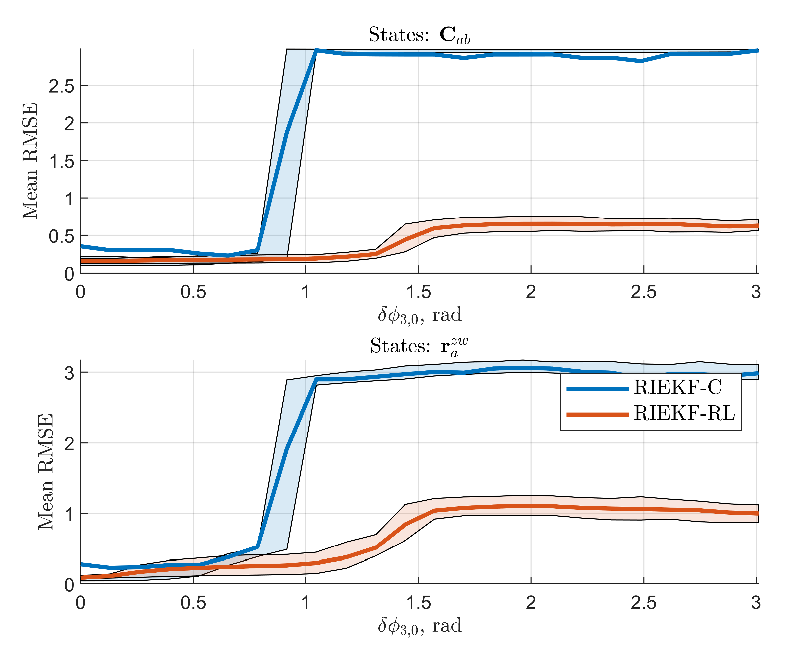
\includegraphics[width=\textwidth]{figs/se3/real/comp_att_rmse_state_Att_RL_C.eps}
		\caption{Mean RMSE for each state.}
	\end{subfigure}
	~
	\begin{subfigure}[b]{0.5\textwidth}
		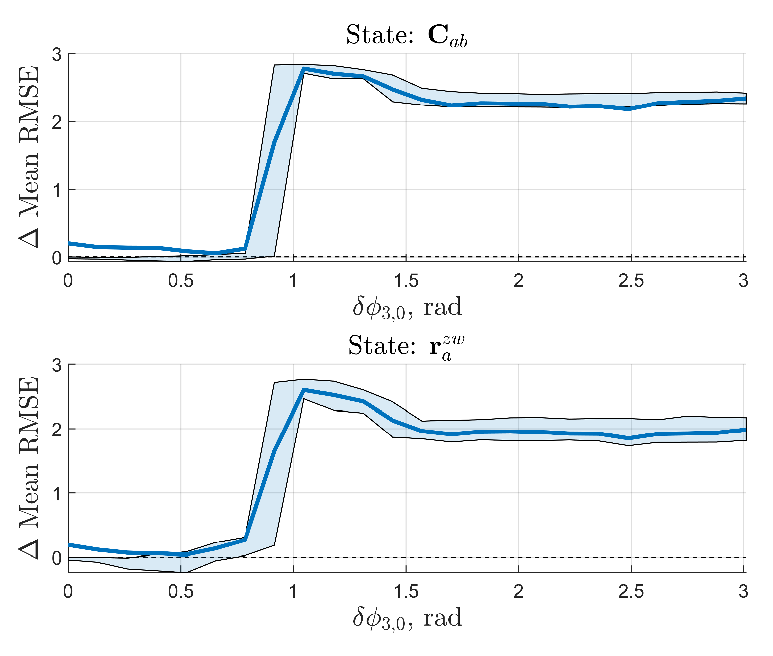
\includegraphics[width=\textwidth]{figs/se3/real/comp_att_diff_state_Att_RL_C.eps}
		\caption{Difference in mean RMSE of MEKF-R and RIEKF.}
	\end{subfigure}
	\caption[Results comparing the RIEKF-C and RIEKF-RL at different initial attitude errors.]{Results of 50 Monte Carlo trials comparing the RIEKF-C and RIEKF-RL at different initial attitude errors.}
	\label{fig:se3_comp_real_att_sim}
\end{figure} 

Based on these results, the error in the initial conditions were drawn from a zero-mean normal distribution with covariance $\mbf{P}_0 = \mathrm{diag}\left(0.1^2 \mbf{1}, \left(\f{\pi}{12}\right)^2\mbf{1}\right)$. The four filters are initially tested in simulation. The results of 500 MC simulations are shown in Figure~\ref{fig:se3_comp_real_sim}, where the error bars capture 80\% of the data. On average, the filters using the pseudo-measurements outperformed the sensors using the camera measurements directly. The RIEKF-C yielded a better attitude estimate than the MEKF-C, but a poorer position estimate.  This trend is repeated in the filters using the pseudo-measurements. However, there is significant spread in the results, as shown by the overlapping error bars. The RIEKF-C did indeed have a lower mean attitude RMSE than the MEKF-C, but it only outperformed the MEKF-C in 51.2\% of the trials. A similar trend is observed in the filters which use pseudo-measurments, where the RIEKF-RL outperformed the MEKF-RL in 53.2\% of the trials. The RIEKF does provide a better attitude estimate than the MEKF on average, but the impact is marginal. Running similar trials on real data reinforced some ideas from simulation. In particular, the MEKFs outperformed the IEKFs in position estimation. Furthermore, there was again little difference in the atittude estimate. These results are shown in Figure~\ref{fig:se3_comp_real}. Despite having a clearly higher mean RMSE, the RIEKF-C outperformed the MEFK-C in 45.6\% of the trials. Similarly, the RIEKF-RL outperformed the MEKF-RL 43\% of the time, the camera-based filters outperform the filters that use the pseudo-measurements.
\begin{figure}
	\centering
	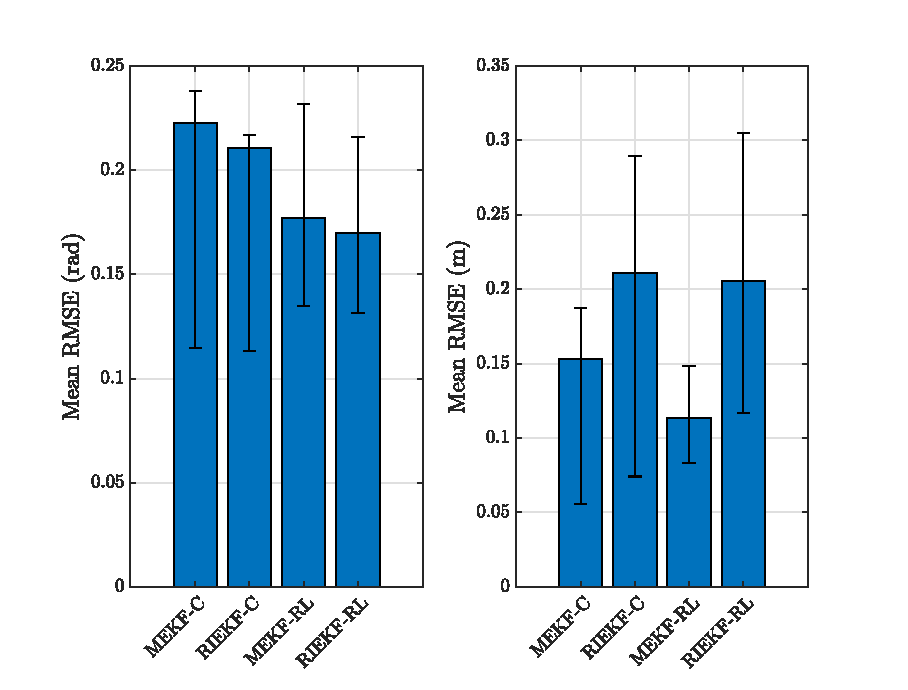
\includegraphics[width=0.7\textwidth]{figs/se3/real/comp_diff_state_sim.eps}
	\caption[Results comparing the MEKF-C, RIEKF-C, MEKF-RL, and RIEKF-RL on simulated data.]{Results of 500 Monte Carlo trials comparing the MEKF-C, RIEKF-C, MEKF-RL, and RIEKF-RL on simulated data. The mean RMSEs in attitude (left) and position (right) are shown.}
	\label{fig:se3_comp_real_sim}
\end{figure}
\begin{figure}
	\centering
	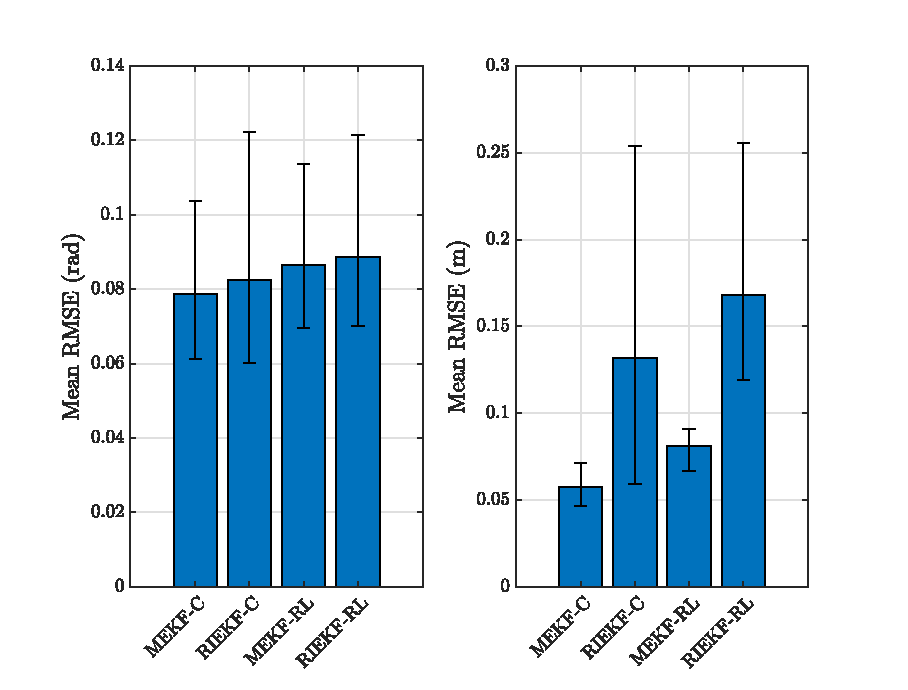
\includegraphics[width=0.7\textwidth]{figs/se3/real/comp_diff_state_Real.eps}
	\caption[Results comparing the MEKF-C, RIEKF-C, MEKF-RL, and RIEKF-RL on real data.]{Results of 500 Monte Carlo trials comparing the MEKF-C, RIEKF-C, MEKF-RL, and RIEKF-RL on real data. The mean RMSEs in attitude (left) and position (right) are shown.}
	\label{fig:se3_comp_real}
\end{figure}

\FloatBarrier

\section{Estimating Bias In the Invariant Framework}

In many estimation problems, sensor biases must be estimated. The IEKF is not particularly well suited for bias estimation, as including bias in the process model destroys the group-affine property. Despite this,  there still may be advantages to estimating bias in the invariant framework. To illustrate this, the sample problem is modified to include a time-varying bias in the rate gyro. For the sake of brevity, only the right-invariant model is shown. The rate gyro measurement model is now
\bdis
	\mbf{u}_b^1 = \mbs{\omega}_b^{ba} - \mbs{\beta}_b - \mbf{w}_b^1,
\edis
where the bias is modelled as a random walk with $\mbsdot{\beta}_b \sim \mc{N}(\mbf{0},\mbf{Q}^3)$.

The state can now be formulated as an element of a new matrix Lie group \cite{Heo2018}, $\mathcal{G}_1$. An element of $\mathcal{G}_1$ is
\bdis
	\mbf{X} = 
	\bma{cccc}
		\mbf{C}_{ab} & \mbf{r}_a^{zw} & & \\
		& 1 & & \\
		& & \mbf{1} & \mbs{\beta}_b\\	
		& & & 1  \\
	\ema.
\edis
The inverse is 
\bdis
	\mbf{X}^{-1} = 
	\bma{cccc}
		\mbf{C}_{ab} & -\mbf{C}_{ab}\mbf{r}_a^{zw} & & \\
		& 1 & & \\
		& & \mbf{1} & -\mbs{\beta}_b\\	
		& & & 1  \\
	\ema.
\edis
Let $\mathfrak{g}_1$ be the matrix Lie algebra of $\mc{G}_1$. The column matrix $\mbs{\xi} \in \mathbb{R}^{9}$ is mapped to $\mathfrak{g}_1$ using
\bdis
	\mbs{\xi}^\wedge = 
	\bma{c}
		\mbs{\xi}^\phi \\
		\mbs{\xi}^\textrm{r} \\
		\mbs{\xi}^\beta \\
	\ema^\wedge
	= 
	\bma{cccc}
		{\mbs{\xi}^\phi}^\times & \mbs{\xi}^\textrm{r} & & \\
		& 0 & & \\
		& & \mbf{0} & \mbs{\xi}^\beta \\	
		& & & 0  \\
	\ema.
\edis
The exponential map from $\mathfrak{g}_1$ to $\mc{G}_1$ is 
\bdis
	\expmapw{\mbs{\xi}} =
	\bma{cccc}
		\exp_{SO(3)}\left({\mbs{\xi}^\phi}^\times\right) & \mbf{J}\mbs{\xi}^\textrm{r} & & \\
		& 1 & & \\
		& & \mbf{1} & \mbs{\xi}^\beta \\	
		& & & 1  \\
	\ema,
\edis
where $\mbf{J}$ is given by \eqref{eq:SE3_Jac}. The adjoint representation of an element of $\mathcal{G}_1$ is
\bdis
	\textrm{Ad}(\mbf{X}) = 
	\bma{ccc}
		\mbf{C}_{ab} & \mbf{0} & \mbf{0} \\
		{\mbf{r}_a^{zw}}^\times\mbf{C}_{ab} & \mbf{C}_{ab} & \mbf{0} \\
		\mbf{0} & \mbf{0} & \mbf{1}
	\ema
\edis 
The kinematics in matrix form are 
\bdis
	\mbfdot{X} = \mbf{X}\mbs{\varpi}^\wedge,
\edis
where 
\bdis
	\mbs{\varpi} =
	\bma{c}
		\mbs{\omega}_b^{ba} \\
		\mbf{v}_b^{zw/a}  \\
		\mbf{0}
	\ema.
\edis
Substituting for the measurement model, 
\bdis
	\mbfdot{X} = \mbf{X}(\mbf{u}_b + \mbf{w}_b)^\wedge, \label{eq:se3_bias_kin}
\edis
where 
\bdis
	\mbf{u}_b =
	\bma{c}
		\mbf{u}_b^1 \\
		\mbf{u}_b^2  \\
		\mbf{0}
	\ema
\edis
and 
\bdis
	\mbf{w}_b =
	\bma{c}
		\mbf{w}_b^1 \\
		\mbf{w}_b^2  \\
		\mbf{w}_b^3
	\ema.
\edis
The kinematics \eqref{eq:se3_bias_kin} are not group affine due to the bias. Therefore, the process model Jacobians will depend on the state estimate. However, using an invariant error definition, the Jacobians can still be derived in a way that causes the Jacobians to be state dependent in different ways. Whether this is advantageous is a question to be answered, at least partially, in this section, and may depend on the problem. It will be tested on the $SE(3)$ sample problem in the right-invariant case, using the measurement model \eqref{eq:se3_meas_right}.

The right-invariant error between some estimated state $\mbfbar{X}$ and the true state $\mbf{X}$ is 
\begin{align*}
	\mbfdel{X} &= \mbfbar{X}\mbf{X}^{-1} \\ 
	&= 
	\bma{cccc}
		\mbfbar{C}_{ab} & \mbfbar{r}_a^{zw} & & \\
		& 1 & & \\
		& & \mbf{1} & \mbsbar{\beta}_b^1\\	
		& & & 1  \\
	\ema
	\bma{cccc}
		\mbf{C}_{ab}^\trans & -\mbf{C}_{ab}\mbf{r}_a^{zw} & & \\
		& 1 & & \\
		& & \mbf{1} & -\mbs{\beta}_b^1\\	
		& & & 1  \\
	\ema \\
	&= 
	\bma{cccc}
		\mbfbar{C}_{ab}\mbf{C}_{ab}^\trans & \mbfbar{r}_a^{zw} - \mbfbar{C}_{ab}\mbf{C}_{ab}^\trans\mbf{r}_a^{zw} & & \\
		& 1 & & \\
		& & \mbf{1} & \mbsbar{\beta}_b^1 -\mbs{\beta}_b^1\\	
		& & & 1  \\
	\ema \\
	&=
	\bma{cccc}
		\mbfdel{C} & \mbfdel{r}  & & \\
		& 1 & & \\
		& & \mbf{1} & \mbsdel{\beta} \\	
		& & & 1  \\
	\ema.
\end{align*}
Defining
\bdis
	\mbfhat{u}_b = 
	\bma{c}	
		\mbf{u}_b^1 + \mbshat{\beta}_b \\
		\mbf{u}_b^2 \\
		\mbf{0}
	\ema,
\edis
the right-invariant error propagation is
\begin{align*}
	\delta \mbfdot{X} &= \dot{\mbfhat{X}}\mbf{X}^{-1} + \mbfhat{X}\mbfdot{X}^{-1} \\ 
	&= \mbfhat{X}\mbfhat{u}_b^\wedge\mbf{X}^{-1} + \mbfhat{X}\mbf{X}^{-1}\mbfdot{X}\mbf{X}^{-1} \\
	&= \mbfhat{X}\mbfhat{u}_b^\wedge\mbf{X}^{-1} + \mbfhat{X}\mbf{X}^{-1}\mbf{X}(\mbf{u}_b + \mbf{w}_b)^\wedge\mbf{X}^{-1} \\
	&= \mbfhat{X}(\mbfhat{u}_b - \mbf{u}_b - \mbf{w}_b)^\wedge\mbf{X}^{-1} \\
	&= \mbfhat{X}(\mbfhat{u}_b - \mbf{u}_b - \mbf{w}_b)^\wedge\mbfhat{X}^{-1}\mbfhat{X}\mbf{X}^{-1} \\
	&= \left(\textrm{Ad}(\mbfhat{X})(\mbfhat{u}_b - \mbf{u}_b - \mbf{w}_b)\right)^\wedge\mbfdel{X}.
\end{align*}
To simplify, let
\begin{align*}
	\mbfdel{u} &= \mbfhat{u}_b - \mbf{u}_b \\
	&= 
	\bma{c}
		\mbf{u}_b^1 + \mbshat{\beta}_b \\
		\mbf{u}_b^2 \\
		\mbf{0}
	\ema -
	\bma{c}
		\mbf{u}_b^1 + \mbs{\beta}_b \\
		\mbf{u}_b^2 \\
		\mbf{0}
	\ema \\
	&=
	\bma{c}
		\mbsdel{\beta} \\
		\mbf{0} \\
		\mbf{0}
	\ema \\
	&= \mbf{B}\mbsdel{\xi},
\end{align*}
where 
\bdis
	\mbf{B} = 
	\bma{ccc}
		\mbf{0} & \mbf{0} & \mbf{1} \\
		\mbf{0} & \mbf{0} & \mbf{0} \\
		\mbf{0} & \mbf{0} & \mbf{0}
	\ema.
\edis
Linearizing by letting $\mbfdel{X} = \mbf{1} + \mbsdel{\xi}^\wedge$ and neglecting second order terms,
\begin{align*}
	\f{\dee}{\dt} \left(\mbf{1} + \mbsdel{\xi}^\wedge\right) &= \left(\textrm{Ad}(\mbfhat{X})(\mbf{B}\mbsdel{\xi} - \mbf{w}_b)\right)^\wedge(\mbf{1} + \mbsdel{\xi}^\wedge), \\
	\delta \mbsdot{\xi}^\wedge &= \left(\textrm{Ad}(\mbfhat{X})(\mbf{B}\mbsdel{\xi} - \mbf{w}_b)\right)^\wedge, \\
	\delta \mbsdot{\xi} &= \textrm{Ad}(\mbfhat{X})\mbf{B}\mbsdel{\xi} - \textrm{Ad}(\mbfhat{X})\mbf{w}_b.
\end{align*}
Therefore, $\mbf{A} = \textrm{Ad}(\mbfhat{X})\mbf{B}$ and $\mbf{L} = -\textrm{Ad}(\mbfhat{X})$. Explicitly,
\bdis
	\mbf{A} = 
	\bma{ccc}
		\mbf{0} & \mbf{0} & \mbfhat{C}_{ab} \\
		\mbf{0} & \mbf{0} & {\mbfhat{r}_a^{zw}}^\times\mbfhat{C}_{ab} \\
		\mbf{0} & \mbf{0} & \mbf{0}
	\ema.
\edis
The matrix $\mbf{A}$ depends on the state estimate because the process model is not group affine.

The innovation associated with the $i^{th}$ landmark is
\begin{align}
	\bma{c} \mbf{z}_k^i \\ \mbf{0} \ema &= \mbfcheck{X}_k\left(\bma{c} \mbf{y}_{b_k}^i \\ 1 \\ \mbf{0} \ema - \bma{c} \mbfcheck{y}_{b_k}^i \\ 1 \\ \mbf{0} \ema\right) \nonumber \\
	&= \mbfcheck{X}_k \left(\mbf{X}_k^{-1} \bma{c} \mbf{r}_a^{p_iw} \\	1 \\ \mbf{0} \ema + \bma{c} \mbf{v}_{b_k} \\ \mbf{0} \ema - \mbfch{X}_k^{-1} \bma{c} \mbf{r}_a^{p_iw} \\ 1  \\ \mbf{0}	\ema \right) \nonumber \\
	&= \delta \mbfch{T}_k \bma{c} \mbf{r}_a^{p_iw} \\	1 \ema + \mbfch{T}_k\bma{c} \mbf{v}_{b_k} \\0 \ema - \bma{c} \mbf{r}_a^{p_iw} \\ 1 \ema. \label{eq:se3_right_bias_3}
\end{align}
Linearizing \eqref{eq:se3_right_bias_3} by letting  $\delta \mbfcheck{X}_k \approx \mbf{1} + \delta \mbscheck{\xi}_k^\wedge$ and $\mbf{v}_{b_k} = \mbfdel{v}_{b_k}$,
\begin{align}
	\bma{c} \mbf{z}_k^i \\ \mbf{0} \ema &\approx \left(\mbf{1} + \delta \mbscheck{\xi}_k^\wedge\right) 
\bma{c}
	\mbf{r}_a^{p_iw} \\
	1 \\
	\mbf{0}
\ema +
\mbfcheck{X}_k
\bma{c}
	\mbfdel{v}_{b_k}^i \\
	\mbf{0}
\ema - 	
\bma{c}
	\mbf{r}_a^{p_iw} \\
	1 \\
	\mbf{0}
\ema \nonumber \\
	& = \delta \mbscheck{\xi}_k^\wedge 
\bma{c}
	\mbf{r}_a^{p_iw} \\
	1 \\
	\mbf{0}
\ema + \mbfcheck{X}_k
\bma{c}
	\mbfdel{v}_{b_k}^i \\
	\mbf{0}
\ema \nonumber \\
	& =  
\bma{cc}
	{\delta\mbscheck{\xi}^{\phi}}^\times & \delta\mbscheck{\xi}_k^\textrm{r} \\
 	\mbf{0} & 0 
\ema 
\bma{c}
	\mbf{r}_a^{p_iw} \\
	1 \\
	\mbf{0}
\ema + \mbfcheck{X}_k
\bma{c}
	\mbfdel{v}_{b_k}^i \\
	\mbf{0}
\ema \nonumber \\
	& =  
\bma{c}
	{\delta\mbscheck{\xi}^{\phi}}^\times\mbf{r}_a^{p_iw} + \delta\mbscheck{\xi}_k^\textrm{r} \\
 	\mbf{0} 
\ema 
 + \mbfcheck{X}_k
\bma{c}
	\mbfdel{v}_{b_k}^i \\
	\mbf{0}
\ema \nonumber \\
	& =  
\bma{c}
	-{\mbf{r}_a^{p_iw}}^\times{\delta\mbscheck{\xi}^{\phi}} + \delta\mbscheck{\xi}_k^\textrm{r} \\
 	\mbf{0} 
\ema 
 + \mbfcheck{X}_k
\bma{c}
	\mbfdel{v}_{b_k}^i \\
	\mbf{0}
\ema \nonumber \\
	& =  
	\mbftilde{H}^i \delta \mbscheck{\xi}_k + \mbfcheck{X}_k
\bma{c}
	\mbfdel{v}_{b_k}^i \\
	\mbf{0}
\ema , \label{eq:se3_right_bias_4}
\end{align}
where 
\bdis
	\mbftilde{H}^i = 
	\bma{ccc}
		-{\mbf{r}_a^{p_iw}}^\times & \mbf{1} & \mbf{0} \\
		\mbf{0} & \mbf{0} & \mbf{0}
	\ema.
\edis
Noting that the bottom row of \eqref{eq:se3_right_bias_4} is always $\mbf{0}$, it can be written
\bdis
	\mbf{z}_k^i = \mbf{H}^i \delta \mbscheck{\xi}_k + \mbf{M}_k^i \mbfdel{v}_{b_k}^i
\edis
where
\bdis
	\mbf{H}^i = 
	\bma{ccc}
		-{\mbf{r}_a^{p_iw}}^\times & \mbf{1} & \mbf{0} \\
	\ema
\edis
and $\mbf{M}_k^i = \mbfch{C}_{ab_k}^\trans$. For the $m$ landmarks,
\beq
	\mbf{H} = \underset{i = 1,\ldots,m}{\textrm{row}}\left(
	\bma{cc}
		-{\mbf{r}_a^{p_iw}}^\times & \mbf{1} \\
	\ema
	\right) \label{eq:se3_H_riekf_bias}
\eeq
and $\mbf{M}_k = \textrm{diag}\left(\mbfcheck{C}_{ab_k}^\trans,\ldots,\mbfcheck{C}_{ab_k}^\trans\right)$. In this case, $\mbf{H}$ is state independent.

\subsection{MEKF Solution}

Similar to Section~\ref{ssec:se3_EKF}, the RIEKF is compared to an MEKF. The MEKF errors are defined as $\mbfdel{C} = \mbfbar{C}_{ab}^\trans\mbf{C}_{ab}$, $\mbfdel{r} = \mbf{r}_a^{zw} - \mbfbar{r}_a^{zw}$, and $\mbsdel{\beta}_b = \mbs{\beta}_b - \mbsbar{\beta}_b$. The MEKF process model Jacobians are
\bdis
	\mbf{A} =
	\bma{ccc} 
		-{\mbf{u}_b^1}^\times & \mbf{0} & \mbf{1} \\
		-\mbfhat{C}_{ab}{\mbf{u}_b^2}^\times & \mbf{0} & \mbf{0} \\
		\mbf{0} & \mbf{0} & \mbf{0}
	\ema
\edis
and $\mbf{L} = \mbf{1}$, while the measurement Jacobians are
\bdis
	\mbf{H}_k = \underset{i = 1,\ldots,m}{\textrm{row}}\left(
	\bma{ccc}
		  \left(\mbfch{C}_{ab_k}^\trans\left( \mbf{r}_a^{p_iw} - \mbfch{r}_a^{z_k^iw} \right)\right)^\times & -\mbfch{C}_{ab_k}^\trans & \mbf{0} \\
	\ema
	\right)
\edis
and $\mbf{M}_k = \mbf{1}$.

\subsection{Simulation Results}

The MEKF and RIEKF are compared in simulation. The noise standard deviations are the same as those in Table~\ref{tab:se3_noises}. In addition, the noise in the bias random walk is assumed isotropic, $\mbf{Q}_k^3 = {\sigma_k^3}^2\mbf{1}$ and is set to $\sigma_k^3 = 0.005\mbf{1}$ \si{rad/s}. The error in the initial conditions were drawn from a zero-mean normal distribution with covariance $\mbf{P}_0 = \mathrm{diag}\left(0.1^2 \mbf{1}, \left(\f{\pi}{4}\right)^2\mbf{1},0.01^2\mbf{1}\right)$. The results obtained from varying the noise in the gyro, velocity sensors, landmark sensor and all the sensors simultaneously  are shown in Figures~\ref{fig:se3_comp_bias_gyro}~to~\ref{fig:se3_comp_bias_all}. On average, the RIEKF outperforms the MEKF, but the improvement is not as stark as when bias wasn't being estimated. This is due to the states now appearing in the process model Jacobian. However, as the measurement model Jacobians are independent of the state estimate, there is still an advantage to using the RIEKF.
\begin{figure}
	\centering
	\begin{subfigure}[b]{0.5\textwidth}
		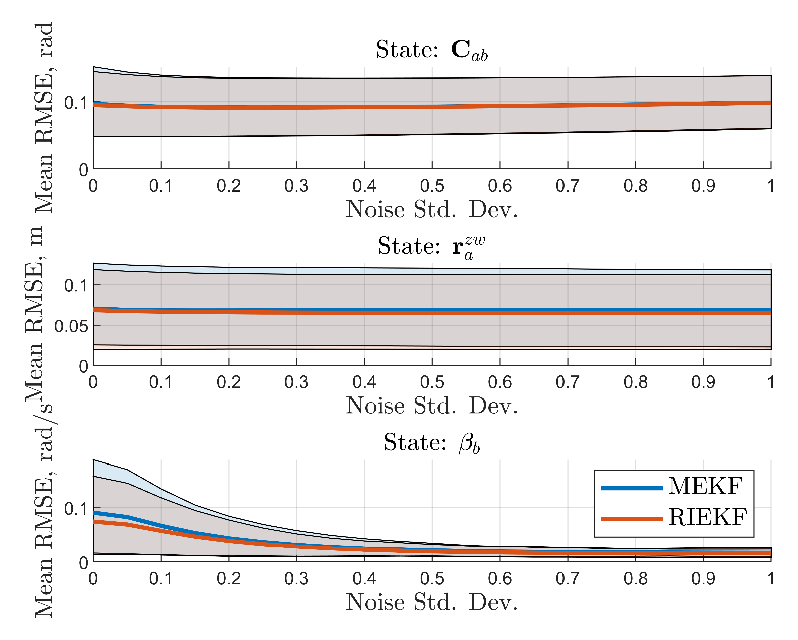
\includegraphics[width=\textwidth]{figs/se3/bias/comp_noise_rmse_state_Bias_Gyro_R.eps}
		\caption{Mean RMSE for each state.}
	\end{subfigure}
	~
	\begin{subfigure}[b]{0.5\textwidth}
		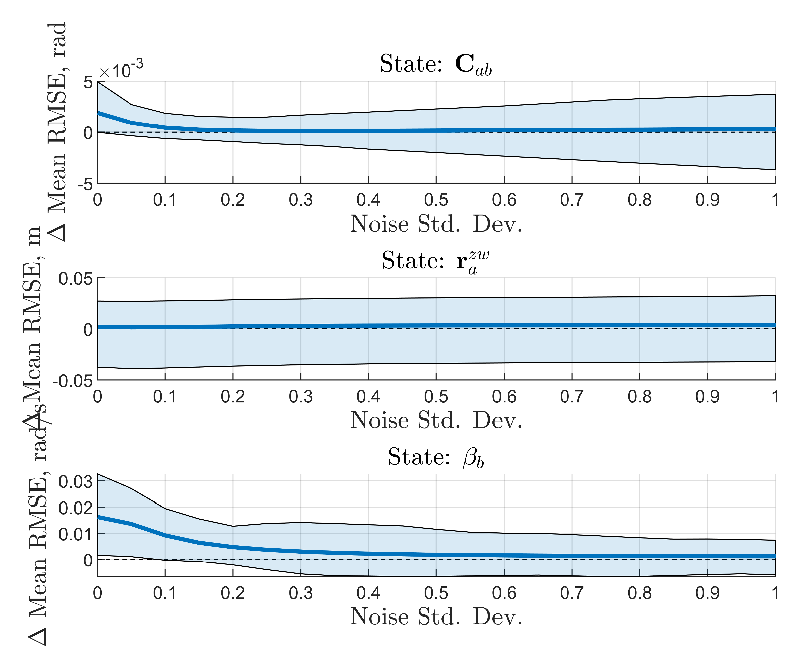
\includegraphics[width=\textwidth]{figs/se3/bias/comp_noise_diff_state_Bias_Gyro_R.eps}
		\caption{Difference in mean RMSE of MEKF and RIEKF.}
	\end{subfigure}
	\caption[Results comparing the MEKF-R and RIEKF varying rate gyro noise.]{Results of 50 Monte Carlo trials comparing the MEKF and RIEKF, where the noise in the rate gyro was varied.}
	\label{fig:se3_comp_bias_gyro}
\end{figure} 

\begin{figure}
	\centering
	\begin{subfigure}[b]{0.5\textwidth}
		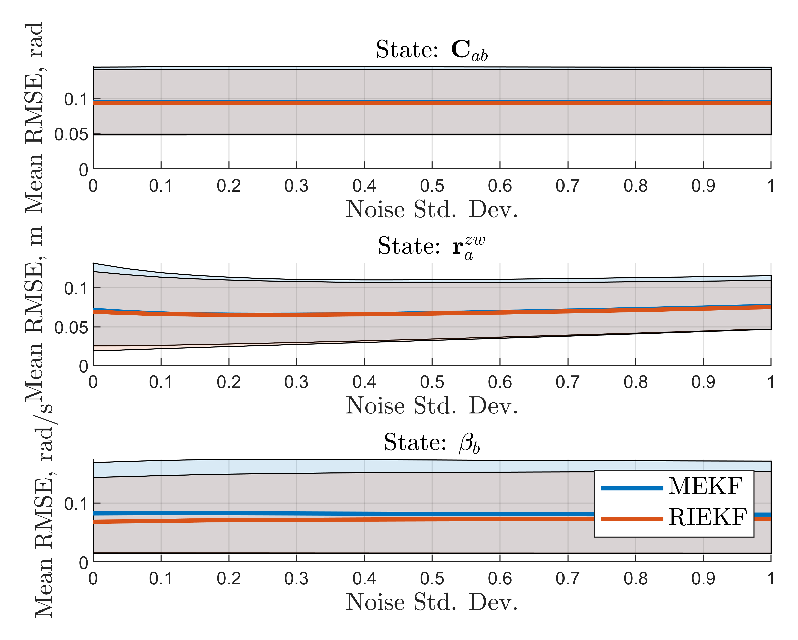
\includegraphics[width=\textwidth]{figs/se3/bias/comp_noise_rmse_state_Bias_Vel_R.eps}
		\caption{Mean RMSE for each state.}
	\end{subfigure}
	~
	\begin{subfigure}[b]{0.5\textwidth}
		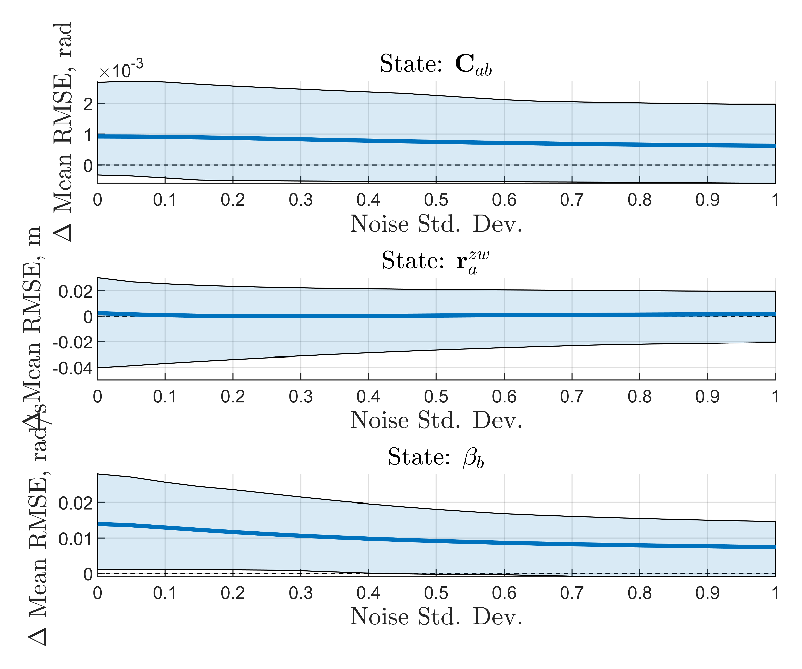
\includegraphics[width=\textwidth]{figs/se3/bias/comp_noise_diff_state_Bias_Vel_R.eps}
		\caption{Difference in mean RMSE of MEKF and RIEKF.}
	\end{subfigure}
	\caption[Results comparing the MEKF-R and RIEKF varying velocity sensor noise.]{Results of 50 Monte Carlo trials comparing the MEKF and RIEKF, where the noise in the velocity sensor was varied.}
	\label{fig:se3_comp_bias_vel}
\end{figure} 


\begin{figure}
	\centering
	\begin{subfigure}[b]{0.5\textwidth}
		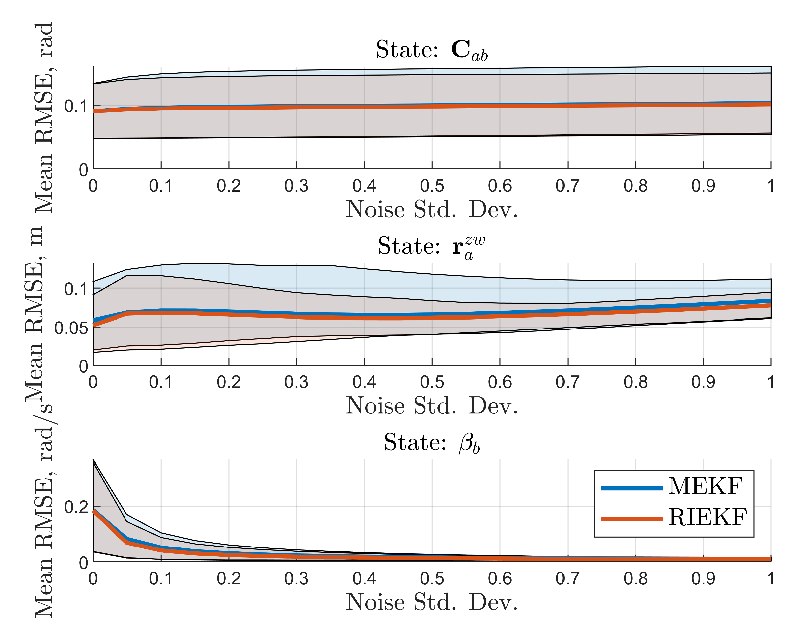
\includegraphics[width=\textwidth]{figs/se3/bias/comp_noise_rmse_state_Bias_Corr_R.eps}
		\caption{Mean RMSE for each state.}
	\end{subfigure}
	~
	\begin{subfigure}[b]{0.5\textwidth}
		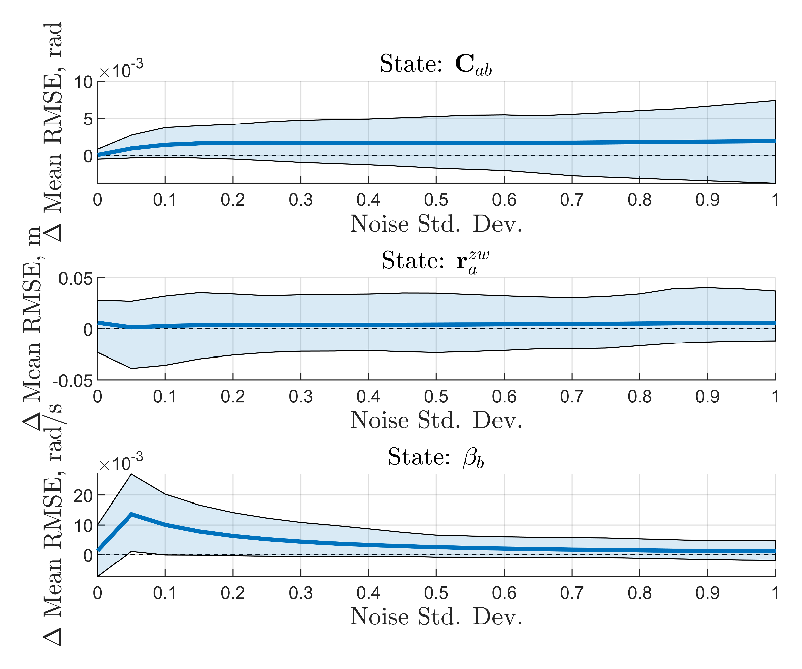
\includegraphics[width=\textwidth]{figs/se3/bias/comp_noise_diff_state_Bias_Corr_R.eps}
		\caption{Difference in mean RMSE of MEKF and RIEKF.}
	\end{subfigure}
	\caption[Results comparing the MEKF-R and RIEKF varying landmark sensor noise.]{Results of 50 Monte Carlo trials comparing the MEKF and RIEKF, where the noise in the landmark sensor was varied.}
	\label{fig:se3_comp_bias_corr}
\end{figure} 

\begin{figure}
	\centering
	\begin{subfigure}[b]{0.5\textwidth}
		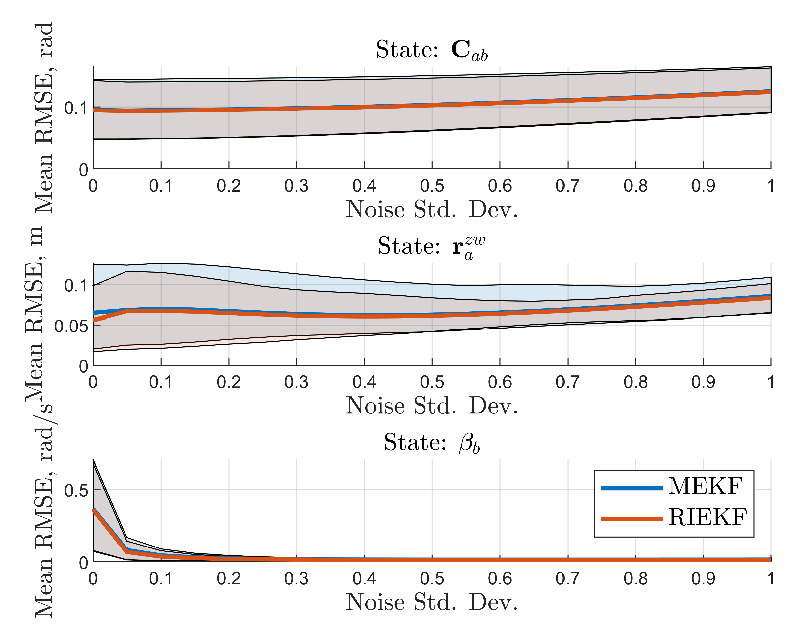
\includegraphics[width=\textwidth]{figs/se3/bias/comp_noise_rmse_state_Bias_All_R.eps}
		\caption{Mean RMSE for each state.}
	\end{subfigure}
	~
	\begin{subfigure}[b]{0.5\textwidth}
		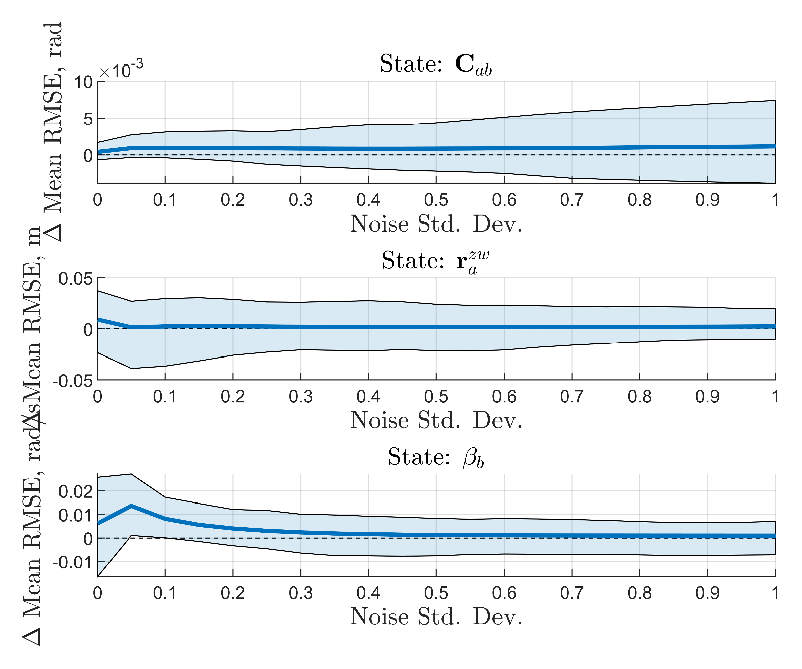
\includegraphics[width=\textwidth]{figs/se3/bias/comp_noise_diff_state_Bias_All_R.eps}
		\caption{Difference in mean RMSE of MEKF and RIEKF.}
	\end{subfigure}
	\caption[Results comparing the MEKF-R and RIEKF varying all sensor noise.]{Results of 50 Monte Carlo trials comparing the MEKF and RIEKF, where the noise in all the sensors varied.}
	\label{fig:se3_comp_bias_all}
\end{figure} 


\section{Conclusion}

In the introduction to this chapter, a set of questions were presented to guide an in-depth discussion on the practical implications of the IEKF. It is useful to revisit these questions at the end of this chapter. 

\begin{enumerate}
	\item \emph{Given a left-invariant measurement model, is it more advantageous to use a LIEKF than an MEKF, and given a right-invariant measurement model, is it more advantageous to use a RIEKF than an MEKF?}
	
	\item \emph{What is the effect of process and measurement noise? How quickly do the convergence properties of the IEKF claimed in \cite{Barrau2017,Barrau2018} break down?}
	
\end{enumerate}

The first two questions posed regarded the perfomance of the IEKF relative to a standard MEKF. In general, over all the experimental trials, the IEKF outperformed the MEKF. However, a more in-depth analysis revealed that much of the improvement could be attributed to better performance in the transient, as it is during this time that the Jacobians in the IEKF are much more accurate than those of the MEKF. During these trials, the effect of sensor noise was also isolated. Despite the convergence properties holding only when noise is negelected, the IEKF is still more effective than the MEKF in the presence of noise.

\begin{enumerate}
	\setcounter{enumi}{2}
	\item \emph{How can the IEKF be used in situations when the measurement model isn't left or right-invariant?}
	
\end{enumerate}

A realistic stereo camera measurement model was used to demonstrate how the IEKF can be used when the measurement model is neither left nor right-invariant. In this scenario, the RIEKF and MEKF provided similar performance, due to the fact that the measurement model was not exactly right-invariant. This was seen both when modifying the IEKF to use the raw measurements, and preprocessing the measurements to create right-invariant pseudomeasurements.

\begin{enumerate}
	\setcounter{enumi}{3}
	\item \emph{How can bias estimation be performed in an invariant framework?}
	
\end{enumerate}

 Lastly, bias estimation was performed in the invariant framework, using results from \cite{Barrau2015}, \cite{Hartley2018} and \cite{Heo2018}. The RIEKF provided better performance than the MEKF, but to a lesser degree than previously shown due to the process model no longer being group affine.

\cleardoublepage
    \chapter{Invariant Batch SLAM}
    \label{chap:batch}
    
In Chapters \ref{chap:IEKF} and \ref{chap:SE3} of this thesis, the IEKF was presented and its practical implications were explored. The IEKF itself relies on three core concepts, namely invariant measurement models, invariant error, and group-affine process models.. When a left-invariant error definition is used in a situation with group-affine kinematics and a left-invariant measurement model, the remarkable properties resulting from the state independence of the Jacobians are recovered. The same can be said for a right-invariant error and a right-invariant measurement model. The properties, however, were only leveraged in the filtering case. In this chapter, batch estimation in an invariant framework is examined. Invariant batch estimation was first done in \cite{Chauchat2018}. It was then applied to visual-inertial odometry in \cite{Hsiung2018} using inertial measurement unit (IMU) preintegration. Here, the landmark-based batch SLAM problem is addressed. This problem differs from the previous work because the landmark positions are being estimated. The chapter is structured as follows. First, the problem is presented, and a standard solution for matrix Lie groups is shown. Next, the invariant framework is applied to the landmark-based batch SLAM solution. Lastly, a sample problem is presented along with simulation results. 

\section{Simultaneous Localization and Mapping on Matrix Lie Groups}
\label{sec:SLAM}

The states of a robotic system are given by $\mbf{X} \in \mathcal{G}$. Typically, only the pose and landmark locations are estimated. Therefore, the estimated states are typically elements of $SE(2)$ or $SE(3)$. However, the theory is applicable to other matrix Lie groups, as is shown here. The location of the $j^{th}$ landmark is typically $\mbf{r}_a^{p_jw}$, where $\rframe{a}$ is some global reference frame, $w$ is a reference point and $p_j$ is the point associated with the $j^{th}$ landmark. Here, to be more concise, they are denoted $\mbf{p}^j \in \mathbb{R}^{n_y}$, $j = 1,\ldots,m$. Estimating the landmark locations and the robots' states at each time step means estimating
\bdis
	\mbf{x} = \left\{\mbf{X}_0,\ldots,\mbf{X}_n,\mbf{p}^1,\ldots,\mbf{p}^m\right\},
\edis
where $t_k \in [t_0,t_n]$.
The discrete-time kinematics are given by
\beq
	\mbf{X}_k = \mbf{F}_{k-1}\left(\mbf{X}_{k-1},\mbf{u}_{k-1},\mbf{w}_{k-1}\right), \label{eq:discrete_process}
\eeq
where $\mbf{u}_{k-1}$ are the interoceptive measurements, or inputs, and $\mbf{w}_{k-1} \sim \mathcal{N}(\mbf{0},\mbf{Q}_{k-1})$ is zero-mean white noise. The exteroceptive measurements are
\bdis
	\mbf{y} = \left\{\mbf{y}_{1,1},\ldots,\mbf{y}_{1,m},\ldots,\mbf{y}_{n,1},\ldots,\mbf{y}_{n,m}\right\},
\edis
where $\mbf{y}_{k,j}$ represents a measurement of the $j^{th}$ landmark at time $t_k$.
The measurements are modelled as
\bdis
	\mbf{y}_{k,j} = \mbf{g}_k\left(\mbf{X}_k,\mbf{p}^j\right) + \mbs{\nu}_{k,j}
\edis
where $\mbs{\nu}_{k,j} \sim \mathcal{N}\left(\mbf{0},\mbf{R}_{k,j}\right)$. A batch maximum \textit{a posteriori} method is be used to solve the SLAM problem.

The SLAM solution is initialized by specifying $\mbfch{X}_0$, the best guess of the initial state. The error in the initial state is then $\mbf{E}_{u,0}(\mbf{x})$. In \cite{Barfoot2017}, a left-invariant error definition is used,
\bdis	
	\expmapw{{\mbf{e}_{u,0}^\textrm{L}}} =  \mbf{E}_{u,0}^\textrm{L}(\mbf{x}) = \mbf{X}_0^{-1}\mbfch{X}_0.
\edis
However, a right-invariant error
\bdis	
	\expmapw{{\mbf{e}_{u,0}^\textrm{R}}} =  \mbf{E}_{u,0}^\textrm{R}(\mbf{x}) = \mbfch{X}_0\mbf{X}_0^{-1}
\edis
can also be used. 

Define the error due to the input to be $\mbf{E}_{u,k}(\mbf{x}) \in \mathcal{G}$. This error can either be left or right invariant. The left-invariant input error is
\beq
	\expmapw{{\mbf{e}_{u,k}^\textrm{L}}} = \mbf{E}_{u,k}^\textrm{L}(\mbf{x}) = \mbfbar{X}_k^{-1} \mbf{F}_{k-1}\left(\mbfbar{X}_{k-1},\mbf{u}_{k-1},\mbf{0}\right), \label{eq:batch_left_input_err}
\eeq
whereas the right-invariant input error is
\beq
	\expmapw{{\mbf{e}_{u,k}^\textrm{R}}} = \mbf{E}_{u,k}^\textrm{R}(\mbf{x}) = \mbf{F}_{k-1}\left(\mbfbar{X}_{k-1},\mbf{u}_{k-1},\mbf{0}\right)\mbfbar{X}_k^{-1}. \label{eq:batch_right_input_err}
\eeq
Here, $\mbfbar{X}_k$ is the nominal state. The measurement error $\mbf{e}_{y,k,j}(\mbf{x})$ is typically defined as
\beq
	\mbf{e}_{y,k,j}(\mbf{x}) = \mbf{y}_{k,j} - \mbf{g}_k\left(\mbf{X}_k,\mbf{p}^j\right). \label{eq:meas_err}
\eeq
Follwing \cite[pp. 127-143]{Barfoot2017}, the SLAM problem is to minimize 
\bdis
	J(\mbf{x}) = \f{1}{2}\mbf{e}_{u,0}(\mbf{x})^\trans\mbf{W}_{u,0}^{-1}\mbf{e}_{u,0}(\mbf{x}) + \f{1}{2}\sum_{k = 1}^n\mbf{e}_{u,k}(\mbf{x})^\trans\mbf{W}_{u,k}^{-1}\mbf{e}_{u,k}(\mbf{x}) + \f{1}{2}\sum_{k = 1}^n\sum_{j = 1}^m\mbf{e}_{y,k,j}(\mbf{x})^\trans\mbf{W}_{y,k,j}^{-1}\mbf{e}_{y,k,j}(\mbf{x}),
\edis
where $\mbf{W}_{u,0}$, $\mbf{W}_{u,k}$, and $\mbf{W}_{y,k,j}$ are weighting matrices related to the probability distribution of the error. The error is deemed Gaussian, as it is assumed that it arises only due to the presence of Gaussian noise in the measurements.  Further defining
\bdis
	\mbf{e}(\mbf{x}) =
	\bma{c}
		\mbf{e}_{u,0}(\mbf{x}) \\
		\vdots \\
		\mbf{e}_{u,n}(\mbf{x})\\
		\hline
		\mbf{e}_{y,1,1}(\mbf{x}) \\
		\mbf{e}_{y,1,2}(\mbf{x}) \\
		\vdots \\
		\mbf{e}_{y,n,m}(\mbf{x})
	\ema,
\edis
and $\mbf{W}_{u} = \textrm{diag}(\mbf{W}_{u,0},\mbf{W}_{u,1},\ldots,\mbf{W}_{u,n})$, $\mbf{W}_y = \textrm{diag}(\mbf{W}_{y,1,1},\mbf{W}_{y,1,2},\mbf{W}_{y,n,m})$ and $\mbf{W} = \textrm{diag}(\mbf{W}_u,\mbf{W}_y)$, the objective function is rewritten as
\bdis
	J(\mbf{x}) = \f{1}{2}\mbf{e}(\mbf{x})^\trans\mbf{W}^{-1}\mbf{e}(\mbf{x}).
\edis
To minimize this objective function, the errors are linearized about an operating point $\mbf{x}^\op$. The linearization is to be done with an uncertainty representation consistent with the choice of error. If a left-invariant error is chosen, the left-invariant uncertainty representation \eqref{eq:left_inv_unc} should be used. If a right-invariant error is chosen, the right-invariant uncertainty representation \eqref{eq:right_inv_unc} should be used. Note that the alternative uncertainty representations given in \eqref{eq:left_unc} and \eqref{eq:right_unc} could also be used. Doing so would simply lead to a change in sign on various Jacobians that, once incorporated into the nonlinear least squares problem, are inconsequential. However, in order to be consistent with the definition of right- or left-invariant error, the uncertainty representations \eqref{eq:left_inv_unc} or \eqref{eq:right_inv_unc} should be used. The linearized prior error has the form
\beq
	\mbf{e}_{u,0}(\mbf{x}) = \mbf{e}_{u,0}(\mbf{x}^\op) - \mbf{F}_0^2\mbsdel{\epsilon}_{0}, \label{eq:e_0}
\eeq
where $\mbsdel{\epsilon}_k$ is the error between the operating and truth trajectory.
The linearized input error has the form
\beq
	\mbf{e}_{u,k}(\mbf{x}) = \mbf{e}_{u,k}(\mbf{x}^\op) + \mbf{F}_k^1\mbsdel{\epsilon}_{k-1} - \mbf{F}_k^2\mbsdel{\epsilon}_k. \label{eq:e_u}
\eeq
The linearized measurement error has the form
\beq
	\mbf{e}_{y,k,j}(\mbf{x}) = \mbf{e}_{y,k,j}(\mbf{x}^\op) - \mbf{H}_{k,j}^1\mbsdel{\epsilon}_{k} - \mbf{H}_{k,j}^2\mbsdel{\zeta}_{j}, \label{eq:e_y}
\eeq
where $\mbsdel{\zeta}_{j}$ is the error  between the operating position estimate and the true position of the $j^{th}$ landmark. Various methods of obtaining \eqref{eq:e_0}, \eqref{eq:e_u}, and \eqref{eq:e_y} are demonstrated in Section~\ref{sec:se23b}. By stacking the estimation errors
\bdis
	\mbfdel{x} =
	\bma{c}
		\mbsdel{\epsilon}_0 \\
		\vdots \\
		\mbsdel{\epsilon}_n \\
		\hline
		\mbsdel{\zeta}_1 \\ 
		\vdots \\
		\mbsdel{\zeta}_m
	\ema,
\edis
the linearized system can then be written 
\bdis
	\mbf{e}(\mbf{x}) = \mbf{e}(\mbf{x}^\op) - \mbs{\Gamma}\mbfdel{x},
\edis
where
\bdis
	\mbs{\Gamma} = 
	\bma{cc}
		\mbf{A}^{-1} & \mbf{0} \\
		\mbf{H}^1 & \mbf{H}^2
	\ema,
\edis
where 
\begin{align*}
	\mbf{A}^{-1} &= 
	\bma{cccc}
		\mbf{F}_0^2    &             &                &              \\
		\mbf{F}_1^1 & \mbf{F}_1^2     &                & 		       \\
		           & \ddots      & \ddots         & 		       \\
		 		   &             & \mbf{F}_{n-1}^1 & \mbf{F}_{n-1}^2       
	\ema, \\
	\mbf{H}^1 &=
	\bma{ccccc}
		& \mbf{H}^1_{1,1} & & & \\
		& \vdots & & & \\
		& \mbf{H}^1_{1,m} & & & \\
		& & \mbf{H}^1_{2,1} & & \\
		& & \vdots & & \\
		& & \mbf{H}^1_{2,m} & & \\
		& & & \ddots & \\
		& & & \ddots & \\
		& & & & \mbf{H}^1_{n,1} \\
		& & & & \vdots \\
		& & & & \mbf{H}^1_{n,m}
	\ema,
\end{align*}
and
\bdis
	\mbf{H}_2 = 
	\bma{ccc}
		\mbf{H}^2_{1,1} & & \\
		& \ddots & \\
		& & \mbf{H}^2_{1,1} \\
		& \vdots & \\
		& \vdots & \\
		\mbf{H}^2_{n,1} & & \\
		& \ddots & \\
		& & \mbf{H}^2_{n,m} \\
		
	\ema.
\edis
The linearized objective function is 
\beq
	J(\mbf{x}^\op + \mbfdel{x}) = (\mbf{e}(\mbf{x}^\op) + \mbs{\Gamma}\mbfdel{x})^\trans\mbf{W}^{-1}(\mbf{e}(\mbf{x}^\op) + \mbs{\Gamma}\mbfdel{x}). \label{eq:batch_lin_cost}
\eeq
Minimizing \eqref{eq:batch_lin_cost} with respect to $\mbfdel{x}$ yields the Gauss-Newton update,
\bdis
	\left(\mbs{\Gamma}^\trans\mbf{W}^{-1}\mbs{\Gamma}\right)\mbfdel{x} = \mbs{\Gamma}^\trans\mbf{W}^{-1}\mbf{e}(\mbf{x}^\op),
\edis
which can be iteratively solved for the minimizing solution $\mbfdel{x}^\star$. The minimizing solution is composed of the state update at every time step, $\mbfdel{x}_k^\star$ and the landmark updates $\mbfdel{x}_j^\star$.

\mymargin{Edited 2020/5/1} 
The operating point is updated using the proper uncertainty representation. If a right-invariant error is used, the state at each time step is updated using
\beq
	\mbf{X}_k = \expmapw{-{\mbfdel{x}_k^\star}}\mbf{X}_k^\op \label{eq:right_update}.
\eeq
If a left-invariant error is used
\beq
	\mbf{X}_k = \mbf{X}_k^\op\expmapw{-{\mbfdel{x}_k^\star}} \label{eq:left_update}.
\eeq
The landmark position estimate is updated using
\bdis
	\mbf{p}^j = {\mbf{p}^j}^\op + \mbfdel{x}_j^\star,
\edis

\section{Leveraging the Invariant Framework in Batch SLAM}
\label{sec:inv_slam}

As was seen in Chapters~\ref{chap:IEKF}~and~\ref{chap:SE3}, a left-invariant error definition, used when the kinematics are group-affine and the measurement model is left-invariant leads to state-independent Jacobians. This is also the case for a right-invariant error definition and right-invariant measurement model. In SLAM, it is typical to have measurement models that are right-invariant, as only information relative to the body of interest is available. Despite this, both the left and right-invariant cases will be considered. In both cases, if the landmark positions were known \textit{a priori}, it would be possible to obtain state-independent Jacobians. However, as the landmark positions are unknown, the best possible result would be to obtain a Jacobian dependent on only the estimated landmark position. This is seen in Section~\ref{sec:se23b}.

\subsection{Left-Invariant Error}

Assume the discrete-time kinematics \eqref{eq:discrete_process} are group-affine, meaning they satisfy \eqref{eq:inv_rel_dis}. The left-invariant error is $\mbfdel{X} = \mbf{X}^{-1}\mbfbar{X}$. The left-invariant input error remains defined as \eqref{eq:batch_left_input_err}. The main difference to consider is the measurement error is now defined
\mymargin{Edited 2021/2/17} 
\bdis
	\mbf{e}_{y,k,j} = \mbfbar{X}_k^{-1}\left(\mbf{y}_{k,j} - \mbf{g}_k(\mbf{X}_k,\mbf{p}^j)\right).
\edis


\subsection{Right-Invariant Error}

Assume the discrete-time kinematics \eqref{eq:discrete_process} are group-affine, meaning they satisfy \eqref{eq:inv_rel_dis}. The right-invariant error is $\mbfdel{X} = \mbfbar{X}\mbf{X}^{-1}$. The right-invariant input error remains defined as \eqref{eq:batch_left_input_err}. The main difference to consider is the measurement error is now defined
\mymargin{Edited 2021/2/17} 
\bdis
	\mbf{e}_{y,k,j} = \mbfbar{X}_k\left(\mbf{y}_{k,j} - \mbf{g}_k(\mbf{X}_k,\mbf{p}^j)\right).
\edis



\section{\NoAutoSpacing Sample Problem 3: Inertial Navigation with Bias}
\label{sec:se23b}

Consider a body moving in 3D space, equipped with an accelerometer, a rate gyro and some sensor that provides relative landmark locations. The problem setup is illustrated in Figure~\ref{fig:se3_prob_landmarks}. Here, $\rframe{a}$ is an inertial frame. The discrete-time kinematics are
\begin{align*}
	\mbf{C}_{ab_k} &= \mbf{C}_{ab_{k-1}}\exp_{SO(3)}\left(T{\mbs{\omega}_{b_{k-1}}^{b_{k-1}a}}^\times\right), \\
	\mbf{v}_a^{z_kw/a} &= \mbf{v}_a^{z_{k-1}w/a} + T(\mbf{C}_{ab_{k-1}}\mbf{f}_{b_{k-1}} + \mbf{g}_a), \\
	\mbf{r}_a^{z_kw} &= \mbf{r}_a^{z_{k-1}w} + T\mbf{v}_a^{z_{k-1}w/a}, 
\end{align*}
where $\mbf{f}_b$ are the specific body forces resolved in $\mathcal{F}_b$ and $\mbf{g}_a$ is the gravity resolved in $\mathcal{F}_a$. The rate gyro model is
\bdis
	\mbf{u}_{b_k}^1 = \mbs{\omega}_{b_k}^{b_ka} - \mbs{\beta}_{b_k}^1 - \mbf{w}_{b_k}^1,
\edis
where $\mbf{w}_{b_k}^1 \sim \mathcal{N}\left(\mbf{0},\mbf{Q}_k^1\right)$. The bias in the rate gyro is modelled as a random walk, $\mbsdot{\beta}_{b_k}^1 \sim \mathcal{N}(\mbf{0},\mbf{Q}_k^3)$. 
The accelerometer model is 
\bdis
	\mbf{u}_{b_k}^2 = \mbf{f}_{b_k} - \mbs{\beta}_{b_k}^2 - \mbf{w}_{b_k}^2,
\edis
where $\mbf{w}^2_{b_k} \sim \mathcal{N}\left(\mbf{0},\mbf{Q}_k^2\right)$. The bias in the accelerometer is modelled as a random walk, $\mbsdot{\beta}_{b_k}^2 \sim \mathcal{N}(\mbf{0},\mbf{Q}_k^4)$. 
The landmark sensor model is
\bdis
	\mbf{y}_k^j = \mbf{C}_{ab_k}^\trans\left(\mbf{r}_{a}^{p_ja} - \mbf{r}_{a}^{z_ka}\right) + \mbs{\nu}_k^j,
\edis
where $\mbs{\nu}_k^j \sim \mathcal{N}(\mbf{0},\mbf{R}_{k,j})$. This is not a realistic measurement model, but is used here to simplify the problem. There may be advantages to this, as was shown in Chapter~\ref{chap:SE3}. To ease the notation, let $\mbf{C}_k = \mbf{C}_{ab_k}$, $\mbf{r}_k = \mbf{r}_a^{z_kw}$, $\mbf{v}_k = \mbf{v}_{a}^{z_kw/a}$, $\mbf{u}_k^i = \mbf{u}_{b_k}^i$, $\mbs{\beta}_k^i = \mbs{\beta}_{b_k}^i$,  $\mbf{w}_k^i = \mbf{w}_{b_k}^i$ and $\mbf{r}_{a}^{p_jw} = \mbf{p}^j$.

\subsection{Matrix Lie Group}

Consider the matrix Lie group $\mathcal{G}_2$, where 
\bdis
	\mbf{X}_k = 
	\bma{cccccc}
		\mbf{C}_k & \mbf{v}_k & \mbf{r}_k & & & \\
		& 1 & & & & \\
		& & 1 & & & \\
		& & & \mbf{1} & \mbs{\beta}_k^1 & \mbs{\beta}_k^2 \\	
		& & & & 1 & \\
		& & & & & 1
	\ema.
\edis
The inverse of an element of $\mc{G}_2$ is 
\bdis
	\mbf{X}_k^{-1} = 
	\bma{cccccc}
		\mbf{C}_k^\trans & -\mbf{C}_k^\trans\mbf{v}_k & -\mbf{C}_k\mbf{r}_k & & \\
		& 1 & & & \\
		& & 1 & & \\
		& & & \mbf{1} & -\mbs{\beta}_k^1 & -\mbs{\beta}_k^2 \\	
		& & & & 1 & \\
		& & & & & 1
	\ema.
\edis
Let $\mathfrak{g}_2$ be the Lie algebra of $\mathcal{G}_2$. The column matrix $\mbs{\xi} \in \mathbb{R}^{15}$ is mapped to $\mathfrak{g}_2$ using
\bdis
	\mbs{\xi}^\wedge = 
	\bma{c}
		\mbs{\xi}^\phi \\
		\mbs{\xi}^\textrm{v} \\
		\mbs{\xi}^\textrm{r} \\
		\mbs{\xi}^1 \\
		\mbs{\xi}^2 \\
	\ema^\wedge
	= 
	\bma{cccccc}
		{\mbs{\xi}^\phi}^\times & \mbs{\xi}^\textrm{v} & \mbs{\xi}^\textrm{r} & & \\
		& 0 & & & &\\
		& & 0 & & & \\
		& & & \mbf{0} & \mbs{\xi}^1 & \mbs{\xi}^2 \\	
		& & & & 0 & \\
		& & & & & 0
	\ema.
\edis
The exponential map from $\mathfrak{g}_2$ to $\mathcal{G}_2$ is 
\bdis
	\expmapw{\mbs{\xi}} = 
	\bma{cccccc}
		\exp_{SO(3)}\left({\mbs{\xi}^\phi}^\times\right) & \mbf{J}\mbs{\xi}^\textrm{v} & \mbf{J}\mbs{\xi}^\textrm{r} & & \\
		& 1 & & &   \\
		& & 1 & & \\
		& & & \mbf{1} & \mbs{\xi}^1 & \mbs{\xi}^2 \\
		& & & & 1 & \\
		& & & & & 1
	\ema,
\edis
where $\mbf{J}$ is given by \eqref{eq:SE3_Jac}.
The adjoint representation of an element of $\mc{G}_2$ is 
\bdis
	\textrm{Ad}(\mbf{X}_k) = 
	\bma{ccccc}
		\mbf{C}_k & & &  \\
		\mbf{v}_k^\times\mbf{C}_k & \mbf{C}_k & &  \\
		\mbf{r}_k^\times\mbf{C}_k & & \mbf{C}_k &  \\
		& & & \mbf{1} &  \\
		& & & & \mbf{1} \\
	\ema.
\edis
The discrete-time kinematics are
\bdis
	\mbf{X}_k = \mbf{F}_{k-1}(\mbf{X}_{k-1})\mbs{\Xi}_{k-1}^\textrm{noisy},
\edis
where 
\bdis
	\mbf{F}_{k-1}(\mbf{X}_{k-1}) =
	\bma{cccccc}
		\mbf{C}_{k-1} & \mbf{v}_{k-1} + T\mbf{g} & \mbf{r}_{k-1} + T\mbf{v}_{k-1} & & \\
		& 1 & & & \\
		& & 1 & & \\
		& & & \mbf{1} & \mbs{\beta}_k^1 & \mbs{\beta}_k^2 \\
		& & & & 1 &  \\
		& & & & & 1
	\ema
\edis
and 
\bdis
	\mbs{\Xi}_{k-1}^\textrm{noisy} =
	\bma{cccccc}
		\exp_{SO(3)}(T({\mbf{u}_{k-1}^1 + \mbs{\beta}_{k-1}^1 + \mbf{w}_{k-1}^1})^\times) & T\left(\mbf{u}_{k-1}^2  + \mbs{\beta}_{k-1}^2 + \mbf{w}_{k-1}^2\right) & \mbf{0} \\
		& 1 & \\
		& & 1 \\
		& & & \mbf{1} & \mbf{w}_{k-1}^3 & \mbf{w}_{k-1}^4  \\
		& & & & 1 & \\
		& & & & & 1
	\ema.
\edis
This will be approximated as
\bdis
	\mbf{X}_k = \mbf{F}_{k-1}(\mbf{X}_{k-1})\mbs{\Xi}_{k-1}\expmapw{\mbf{w}_{k-1}},
\edis
where $\mbf{w}_{k-1} = \; [ \; {\mbf{w}_{k-1}^1}^\trans \; \; {\mbf{w}_{k-1}^2}^\trans \; \; \mbf{0} \; \; {\mbf{w}_{k-1}^3}^\trans \; \; {\mbf{w}_{k-1}^4}^\trans \; ]^\trans \sim \mathcal{N}(\mbf{0},\mbf{Q}_{k-1})$,
\bdis
	\mbs{\Xi}_{k-1} =
	\bma{cccccc}
		\mbs{\Psi}_{k-1} & T\left(\mbf{u}_{k-1}^2  + \mbs{\beta}_{k-1}^2\right) & \mbf{0} \\
		& 1 & \\
		& & 1 \\
		& & & \mbf{1} & \mbf{0} & \mbf{0}  \\
		& & & & 1 & \\
		& & & & & 1
	\ema,
\edis
and $\mbs{\Psi}_{k-1} = \exp_{SO(3)}(T({\mbf{u}_{k-1}^1} + \mbs{\beta}_{k-1}^1)^\times)$. The noise covariance is $\mbf{Q}_{k-1} = \textrm{diag}\left(\mbf{Q}_{k-1}^1,\mbf{Q}_{k-1}^2,\mbf{0},\mbf{Q}_{k-1}^3,\mbf{Q}_{k-1}^4\right)$. The measurement model is
\bdis
	\mbf{y}_{k,j} = \mbf{C}_k^\trans(\mbf{p}^j - \mbf{r}_k) + \mbs{\nu}_{k,j},
\edis 
where $\mbs{\nu}_{k,j} \sim \mathcal{N}(\mbf{0},\mbf{R}_{k,j})$. It can be represented using an element of $\mathcal{G}_2$ as
\beq
	\mbftilde{y}_{k,j} = \mbf{X}_k^{-1} \bma{c} \mbf{p}^j \\ 0 \\ 1 \\ \mbf{0} \ema + \mbstilde{\nu}_{k,j}, \label{eq:meas_model_X_se23b}
\eeq
where $\mbftilde{y}_{k,j} =  [ \; \mbf{y}_{k,j}^\trans \; 0 \; 1 \; \mbf{0} \;]^\trans$ and $\mbstilde{\nu}_{k,j} = [ \; \mbs{\nu}_{k,j}^\trans \; \mbf{0} \; ]^\trans$.

Six different approaches are compared. First, a standard left-invariant error definition is used, as the one described in Section~\ref{sec:SLAM}. The left-invariant error derivation is then changed in a way that leads to Jacobians dependent only on the measurement and not on the state. Next, the right-invariant error definition is used. Lastly, these three aforementioned approaches are repeated, using the appropriate invariant measurement error as shown in Section~\ref{sec:inv_slam}. Tables~\ref{tab:slam_input}~and~\ref{tab:slam_meas} summarize the various approaches.
\begin{table}[]
\resizebox{\textwidth}{!}{%
\centering
\renewcommand{\arraystretch}{1.75}
\begin{tabular}{|l|l|l|l|l|}
\hline
 App. & $\mbf{E}_{u,k}$                                             & $\mbf{W}_{u,k}$ & $\mbf{F}_k^1$ & $\mbf{F}_k^2$  \\ \hhline{|=|=|=|=|=|} 
1        & $\mbf{X}_k^{-1}\mbf{F}_{k-1}\mbs{\Xi}_{k-1}$ & $\mbf{Q}_k$  &  $\mathrm{Ad}({\mbf{X}_k^\op}^{-1}\mbf{F}_{k-1}^\op)\mbf{B}^\textrm{L} + \mbf{D}_{k-1}^\textrm{L}$ & $-\mbf{1}$  \\ \hline
2 & $\mbf{X}_k^{-1}\mbf{F}_{k-1}\mbs{\Xi}_{k-1}$ & $\mbf{Q}_k$ &  $\mathrm{Ad}({\mbs{\Xi}_{k-1}^\op}^{-1})\mbf{B}^\textrm{L} + \mbf{D}_{k-1}^\textrm{L}$ & $-\mbf{1}$ \\ \hline       
3 & $\mbf{F}_{k-1}\mbs{\Xi}_{k-1}\mbf{X}_k^{-1}$        &  $\mathrm{Ad}(\mbfbar{F}_{k-1}\mbs{\Xi}_{k-1})\mbf{Q}_k\mathrm{Ad}(\mbfbar{F}_{k-1}\mbs{\Xi}_{k-1})^\trans$ & $\mbf{B}^\textrm{R} + \mathrm{Ad}(\mbf{F}_{k-1}^\op)\mbf{D}_{k-1}^\textrm{R}$   &  $-\mbf{1}$ \\ \hline
4        & $\mbf{X}_k^{-1}\mbf{F}_{k-1}\mbs{\Xi}_{k-1}$ & $\mbf{Q}_k$  &  $\mathrm{Ad}({\mbf{X}_k^\op}^{-1}\mbf{F}_{k-1}^\op)\mbf{B}^\textrm{L} + \mbf{D}_{k-1}^\textrm{L}$ & $-\mbf{1}$  \\ \hline
5        & $\mbf{X}_k^{-1}\mbf{F}_{k-1}\mbs{\Xi}_{k-1}$ & $\mbf{Q}_k$ &  $\mathrm{Ad}({\mbs{\Xi}_{k-1}^\op}^{-1})\mbf{B}^\textrm{L} + \mbf{D}_{k-1}^\textrm{L}$ & $-\mbf{1}$ \\ \hline
6        & $\mbf{F}_{k-1}\mbs{\Xi}_{k-1}\mbf{X}_k^{-1}$        &  $\mathrm{Ad}(\mbfbar{F}_{k-1}\mbs{\Xi}_{k-1})\mbf{Q}_k\mathrm{Ad}(\mbfbar{F}_{k-1}\mbs{\Xi}_{k-1})^\trans$ & $\mbf{B}^\textrm{R} + \mathrm{Ad}(\mbf{F}_{k-1}^\op)\mbf{D}_{k-1}^\textrm{R}$   &  $-\mbf{1}$ \\ \hline
\end{tabular}}
\captionsetup{justification = justified}
\caption[Summary of input errors and Jacobians for the 6 different approaches.]{Summary of input errors and Jacobians for the 6 different approaches. Approach 1 uses the standard left-invariant approach with the type 1 Jacobians, while Approach 2 uses the type 2 Jacobians. Approach 3 uses the right-invariant error. Approaches 4, 5, and 6 replicate Approaches 1, 2, and 3, substituting the regular measurement error for an invariant measurement error.}
\label{tab:slam_input}
\end{table}


\begin{table}[]
\centering
\renewcommand{\arraystretch}{1.5}
\begin{tabular}{|l|l|l|l|l|}
\hline
 App. & $\mbftilde{e}_{y,k,j}$                                             & $\mbf{W}_{y,k,j}$ & $\mbf{H}_{k,j}^1$ & $\mbf{H}_{k,j}^2$ \\ \hhline{|=|=|=|=|=|}
1        & $\mbftilde{y}_k^j - \mbf{X}_k^{-1}\mbftilde{p}^j$ & $\mbf{R}_{k,j}$  &  $-\bma{ccccc} \left({\mbf{C}_k^\op}^\trans({\mbf{p}^j}^\op - \mbf{r}_k^\op)\right)^\times & \mbf{0} & -\mbf{1} & \mbf{0} & \mbf{0} \ema $ & ${\mbf{C}_k^\op}^\trans$  \\ \hline
2       & $\mbftilde{y}_k^j - \mbf{X}_k^{-1}\mbftilde{p}^j$ & $\mbf{R}_{k,j}$  &  $-\bma{ccccc} \left({\mbf{C}_k^\op}^\trans({\mbf{p}^j}^\op - \mbf{r}_k^\op)\right)^\times & \mbf{0} & -\mbf{1} & \mbf{0} & \mbf{0} \ema $ & ${\mbf{C}_k^\op}^\trans$  \\ \hline\
3         & $\mbftilde{y}_k^j - \mbf{X}_k^{-1}\mbftilde{p}^j$ & $\mbf{R}_{k,j}$  &  $-\bma{ccccc} {\mbf{C}_k^\op}^\trans{{\mbf{p}^j}^\op}^\times & \mbf{0} & -{\mbf{C}_k^\op}^\trans & \mbf{0} & \mbf{0} \ema $ & ${\mbf{C}_k^\op}^\trans$  \\ \hline
4         & $\mbfbar{X}_k(\mbftilde{y}_k^j - \mbf{X}_k^{-1}\mbftilde{p}^j)$ & $\mbfbar{C}_k\mbf{R}_{k,j}\mbfbar{C}_k^\trans$  &  $-\bma{ccccc} ({\mbf{p}^j}^\op - \mbf{r}_k^\op)^\times\mbf{C}_k^\op & \mbf{0} & -\mbf{C}_k^\op & \mbf{0} & \mbf{0} \ema $ & $\mbf{1}$  \\ \hline
5         & $\mbfbar{X}_k(\mbftilde{y}_k^j - \mbf{X}_k^{-1}\mbftilde{p}^j)$ & $\mbfbar{C}_k\mbf{R}_{k,j}\mbfbar{C}_k^\trans$  &  $-\bma{ccccc} ({\mbf{p}^j}^\op - \mbf{r}_k^\op)^\times\mbf{C}_k^\op & \mbf{0} & -\mbf{C}_k^\op & \mbf{0} & \mbf{0} \ema $ & $\mbf{1}$  \\ \hline
6        & $\mbfbar{X}_k^{-1}(\mbftilde{y}_k^j - \mbf{X}_k^{-1}\mbftilde{p}^j)$ & $\mbfbar{C}_k^\trans\mbf{R}_{k,j}\mbfbar{C}_k$  &  $-\bma{ccccc} {{\mbf{p}^j}^\op}^\times & \mbf{0} & -\mbf{1} & \mbf{0} & \mbf{0} \ema $ & $\mbf{1}$  \\ \hline
\end{tabular}
\captionsetup{justification = justified}
\caption[Summary of input errors and Jacobians for the 6 different approaches.]{Summary of input errors and Jacobians for the 6 different approaches. Approach 1 uses the standard left-invariant approach with the type 1 Jacobians, while Approach 2 uses the type 2 Jacobians. Approach 3 uses the right-invariant error. Approaches 4, 5, and 6 replicate Approaches 1, 2, and 3, substituting the regular measurement error for an invariant measurement error.}
\label{tab:slam_meas}
\end{table}


\subsection{\NoAutoSpacing Approach 1: Left-Invariant Error Definition with Type 1 Jacobians}
\label{ssec:se23b_left}

Let the error be defined as $\mbfdel{X} = \mbf{X}^{-1}\mbfbar{X}$. The uncertainty representation is $\mbf{X} = \mbfbar{X}\exp\left(-\mbsdel{\xi}^\wedge\right)$. Therefore the state is updated using \eqref{eq:left_update}. The left-invariant error in the state is
\begin{align*}
	\mbf{X}_k^{-1}\mbfbar{X}_k &=  
	\bma{cccccc}
		\mbf{C}_k^\trans & -\mbf{C}_k^\trans\mbf{v}_k & -\mbf{C}_k\mbf{r}_k & & \\
		& 1 & & & \\
		& & 1 & & \\
		& & & \mbf{1} & -\mbs{\beta}_k^1 & -\mbs{\beta}_k^2 \\	
		& & & & 1 & \\
		& & & & & 1
	\ema 
	\bma{cccccc}
		\mbfbar{C}_k & \mbfbar{v}_k & \mbfbar{r}_k & & & \\
		& 1 & & & & \\
		& & 1 & & & \\
		& & & \mbf{1} & \mbsbar{\beta}_k^1 & \mbsbar{\beta}_k^2 \\	
		& & & & 1 & \\
		& & & & & 1
	\ema \\
	&= 
	\bma{cccccc}
		\mbf{C}_k^\trans\mbfbar{C}_k & \mbf{C}_k^\trans(\mbfbar{v}_k - \mbf{v}_k) &  \mbf{C}_k^\trans(\mbfbar{r}_k - \mbf{r}_k) & & & \\
		& 1 & & & &\\
		& & 1 &	& & \\
		& & & \mbf{1} & \mbsbar{\beta}_k^1 - \mbs{\beta}_k^1 & \mbsbar{\beta}_k^2  -\mbs{\beta}_k^2\\	
		& & & & 1 & \\
		& & & & & 1
	\ema \\
	&= \bma{cccccc}
		\mbfdel{C}_k & \mbfdel{v}_k &  \mbfdel{r}_k \\
		& 1 & \\
		& & 1 \\
		& & & \mbf{1} & \mbsdel{\beta}_k^1 & \mbsdel{\beta}_k^2 \\	
		& & & & 1 & \\
		& & & & & 1
	\ema.
\end{align*}
Thus, the perturbation in $\mathbb{R}^{15}$ is defined as
\bdis
	\mbsdel{\xi}_k = 
	\bma{c}
		\log_{SO(3)}(\mbfdel{C}_k)^\vee \\
		\mbf{J}_k^{-1}\mbfdel{v}_k \\
		\mbf{J}_k^{-1}\mbfdel{r}_k \\
		\mbsdel{\beta}_k^1 \\
		\mbsdel{\beta}_k^2 \\
	\ema.
\edis

The left-invariant error in $\mbf{F}_{k}(\mbf{X}_{k})$ is
\begin{align*}
	\mbfdel{F}_k &= \mbf{F}_k(\mbf{X}_k)^{-1}\mbf{F}_{k}(\mbfbar{X}_k) \\
	&= 
	\bma{cccccc}
		\mbf{C}_{k}^\trans & -\mbf{C}_{k}^\trans\left(\mbf{v}_{k} + T\mbf{g}\right) & -\mbf{C}_{k}^\trans\left(\mbf{r}_{k} + T\mbf{v}_{k}\right) \\
		& 1 & \\
		& & 1 \\
		& & & \mbf{1} & -\mbs{\beta}_k^1 & -\mbs{\beta}_k^2 \\
		& & & & 1 &  \\
		& & & & & 1
	\ema \\
	& \qquad \qquad \qquad \qquad \qquad \qquad \qquad \qquad \qquad
	\bma{cccccc}
		\mbfbar{C}_{k} & \mbfbar{v}_{k} + T\mbf{g} & \mbfbar{r}_{k} + T\mbfbar{v}_{k} \\
		& 1 & \\
		& & 1 \\
		& & & \mbf{1} & \mbsbar{\beta}_k^1 & \mbsbar{\beta}_k^2 \\
		& & & & 1 &  \\
		& & & & & 1
	\ema \\
	&= 
	\bma{cccccc}
		\mbf{C}_{k}^\trans\mbfbar{C}_{k} & \mbf{C}_{k}^\trans\left(\mbfbar{v}_{k} - \mbf{v}_{k}\right) & \mbf{C}_{k}^\trans\left(\mbfbar{r}_{k} + T\mbfbar{v}_{k} - \mbf{r}_{k} - T\mbf{v}_{k}\right) \\
		& 1 & \\
		& & 1 \\
		& & & \mbf{1} & \mbsbar{\beta}_k^1 - \mbs{\beta}_k^1 & \mbsbar{\beta}_k^2 - \mbs{\beta}_k^2 \\
		& & & & 1 &  \\
		& & & & & 1
	\ema \\
	&= 
	\bma{cccccc}
		\mbfdel{C}_k & \mbfdel{v}_k & \mbf{C}_{k}^\trans\left(\mbfbar{r}_{k} - \mbf{r}_{k}\right) + T\mbf{C}_{k}^\trans\left( \mbfbar{v}_{k} -  \mbf{v}_{k}\right) \\
		& 1 & \\
		& & 1 \\
		& & & \mbf{1} & \mbsdel{\beta}_k^1 & \mbsdel{\beta}_k^2  \\
		& & & & 1 &  \\
		& & & & & 1
	\ema \\
	&= 
	\bma{cccccc}
		\mbfdel{C}_k & \mbfdel{v}_k & \mbfdel{r}_k + T\mbfdel{v}_k \\
		& 1 & \\
		& & 1 \\
		& & & \mbf{1} & \mbsdel{\beta}_k^1 & \mbsdel{\beta}_k^2  \\
		& & & & 1 &  \\
		& & & & & 1
	\ema
\end{align*}
As $\mbfdel{F}_k \in \mathcal{G}_2$, it can be written using the exponential map as $\mbfdel{F}_k = \exp\left(\mbfdel{f}_k^\wedge\right)$, where
\bdis
	\mbfdel{f}_k = 
	\bma{c}
		\log_{SO(3)}(\mbfdel{C}_k)^\vee \\
		\mbf{J}_k^{-1}\mbfdel{v}_k \\
		\mbf{J}_k^{-1}\left(\mbfdel{r}_k + T\mbfdel{v}_k\right) \\
		\mbsdel{\beta}_k^1 \\
		\mbsdel{\beta}_k^2
	\ema.
\edis
This can be rewritten as  $\mbfdel{f}_k = \mbf{B}^\textrm{L}\mbsdel{\xi}_k$, where
\bdis
	\mbf{B}^\textrm{L} =
	\bma{ccccc}	
		\mbf{1} & \mbf{0} & \mbf{0} & \mbf{0} & \mbf{0}  \\
		\mbf{0} & \mbf{1} & \mbf{0} & \mbf{0} & \mbf{0} \\
		\mbf{0} & T\mbf{1} & \mbf{1}& \mbf{0} & \mbf{0} \\
		\mbf{0} & \mbf{0} & \mbf{0}& \mbf{1} & \mbf{0} \\
		\mbf{0} & \mbf{0} & \mbf{0}& \mbf{0} & \mbf{1} \\
	\ema.
\edis
As $\mbs{\Xi}_{k} \in \mathcal{G}_2$ is state-dependent, it has an associated left-invariant error, which is $\mbsdel{\Xi}_k = \mbs{\Xi}_k^{-1}\mbsbar{\Xi}_k$. Letting $\mbsbar{\Psi}_k = \exp_{SO(3)}\left(T(\mbf{u}_k^1 + \mbsbar{\beta}_k^1)^\times\right)$, the left-invariant error is
\begin{align*}
	\mbsdel{\Xi}_k &= \mbs{\Xi}_k^{-1}\mbsbar{\Xi}_k \\
	&= 
	\bma{cccccc}
		\mbs{\Psi}_k^\trans & -T\mbs{\Psi}_k^\trans(\mbf{u}_k^2 + \mbs{\beta}_k^2) & \mbf{0} & & \\
		& 1 & & &\\
		& & 1 & & &  \\
		& & & \mbf{1} & \mbf{0} & \mbf{0}  \\
		& & & & 1 & \\
		& & & & & 1
	\ema 
	\bma{cccccc}
		\mbsbar{\Psi}_k & T(\mbf{u}_k^2 + \mbsbar{\beta}_k^2) & \mbf{0} & & \\
		& 1 & & & \\
		& & 1 & & &  \\
		& & & \mbf{1} & \mbf{0} & \mbf{0}  \\
		& & & & 1 & \\
		& & & & & 1
	\ema \\
	&= 
	\bma{cccccc}
		\mbs{\Psi}_k^\trans\mbsbar{\Psi}_k & T\mbs{\Psi}_k^\trans(\mbf{u}_k^2 + \mbsbar{\beta}_k^2) -T\mbs{\Psi}_k^\trans(\mbf{u}_k^2 + \mbs{\beta}_k^2) & \mbf{0} & &  \\
		& 1 & & & & \\
		& & 1 & & & \\
		& & & \mbf{1} & \mbf{0} & \mbf{0}  \\
		& & & & 1 & \\
		& & & & & 1
	\ema \\
	&= 
	\bma{cccccc}
		\mbs{\Psi}_k^\trans\mbsbar{\Psi}_k & T\mbs{\Psi}_k^\trans(\mbsbar{\beta}_k^2 - \mbs{\beta}_k^2) & \mbf{0}  & &  \\
		& 1 & & & & \\
		& & 1 & & & \\
		& & & \mbf{1} & \mbf{0} & \mbf{0}  \\
		& & & & 1 & \\
		& & & & & 1
	\ema \\
	&\approx 
	\bma{cccccc}
		\exp_{SO(3)}\left(-T(\mbs{\beta}_k^1 - \mbsbar{\beta}_k^1)^\times\right)  & T\mbs{\Psi}_k^\trans\mbsdel{\beta}_k^2 & \mbf{0} & &  \\
		& 1 & & & & \\
		& & 1 & & & \\
		& & & \mbf{1} & \mbf{0} & \mbf{0}  \\
		& & & & 1 & \\
		& & & & & 1
	\ema \\
	&= 
	\bma{cccccc}
		\exp_{SO(3)}\left(T{\mbsdel{\beta}_k^1}^\times\right) & T\mbs{\Psi}_k^\trans\mbsdel{\beta}_k^2  & \mbf{0} & \\
		& 1 & & & & \\
		& & 1 & & & \\
		& & & \mbf{1} & \mbf{0} & \mbf{0}  \\
		& & & & 1 & \\
		& & & & & 1
	\ema.
\end{align*}
To simplify, let $\mbs{\Psi}_k^\trans = \exp_{SO(3)}\left(T{\mbsdel{\beta}_k^1}^\times\right)\mbsbar{\Psi}_k^\trans$, and linearize by letting $\exp_{SO(3)}\left(T{\mbsdel{\beta}_k^1}^\times\right) \approx \mbf{1} + T{\mbsdel{\beta}_k^1}^\times$ and neglecting second order terms. Then,
\begin{align*}
	\mbsdel{\Xi}_k &= 		
	\bma{cccccc}
		\exp_{SO(3)}\left(T{\mbsdel{\beta}_k^1}^\times\right) & T\exp_{SO(3)}\left(T{\mbsdel{\beta}_k^1}^\times\right)\mbsbar{\Psi}_k^\trans\mbsdel{\beta}_k^2  & \mbf{0} & \\
		& 1 & & & & \\
		& & 0 & & & \\
		& & & \mbf{1} & \mbf{0} & \mbf{0}  \\
		& & & & 1 & \\
		& & & & & 1
	\ema \\
	&\approx \bma{cccccc}
		\exp_{SO(3)}\left(T{\mbsdel{\beta}_k^1}^\times\right) & T(\mbf{1} + T{\mbsdel{\beta}_k^1}^\times)\mbsbar{\Psi}_k^\trans\mbsdel{\beta}_k^2  & \mbf{0} & \\
		& 1 & & & & \\
		& & 1 & & & \\
		& & & \mbf{1} & \mbf{0} & \mbf{0}  \\
		& & & & 1 & \\
		& & & & & 1
	\ema \\
		&= \bma{cccccc}
		\exp_{SO(3)}\left(T{\mbsdel{\beta}_k^1}^\times\right) & T\mbsbar{\Psi}_k^\trans\mbsdel{\beta}_k^2  &  \mbf{0}& \\
		& 1 &  & & & \\
		& & 1 & & & \\
		& & & \mbf{1} & \mbf{0} & \mbf{0}  \\
		& & & & 1 & \\
		& & & & & 1
	\ema.
\end{align*}
As $\mbsdel{\Xi}_k \in \mathcal{G}_2$, it can be expressed using the exponential map as $\mbsdel{\Xi}_k = \expmapw{\mbfdel{u}_k}$, where
\bdis
	\mbfdel{u}_k =
	\bma{c} 
		T\mbsdel{\beta}_k^1 \\
		T\mbf{J}^{-1}\mbsbar{\Psi}_k^\trans\mbsdel{\beta}_k^2 \\
		\mbf{0}
	\ema.
\edis 
This can be rewritten as $\mbfdel{u}_k = \mbf{D}_{k}^\textrm{L}\mbsdel{\xi}_k$, where 
\bdis
	\mbf{D}_{k}^\textrm{L} =
	\bma{ccccc}	
		\mbf{0} & \mbf{0} & \mbf{0} & T\mbf{1} & \mbf{0} \\
		\mbf{0} & \mbf{0} & \mbf{0} & \mbf{0} & T\mbsbar{\Psi}_k^\trans \\
		\mbf{0} & \mbf{0} & \mbf{0} & \mbf{0} & \mbf{0} \\
		\mbf{0} & \mbf{0} & \mbf{0} & \mbf{0} & \mbf{0} \\
		\mbf{0} & \mbf{0} & \mbf{0} & \mbf{0} & \mbf{0}
	\ema.
\edis


\subsubsection{Probability Distribution of the Errors}

The prior error probability distribution is found by linearizing $\mbf{E}_{u,0} = \mbf{X}_0^{-1}\mbfbar{X}_0$. Letting $\mbf{X}_0 = \mbfbar{X}_0\expmapw{-\mbsdel{\xi}_0}$, the prior input error is
\begin{align*}
	\mbf{E}_{u,0}(\mbf{x}) &= \mbf{X}_0^{-1}\mbfbar{X}_0, \\
	\exp\left(\mbf{e}_{u,0}^\wedge\right) &= \exp\left(\mbsdel{\xi}_0^\wedge\right)\mbfbar{X}_0^{-1}\mbfbar{X}_0 \\
	&= \exp\left(\mbsdel{\xi}_0^\wedge\right), \\
	\mbf{e}_{u,0}^\wedge &\approx \mbsdel{\xi}_0^\wedge, \\
	\mbf{e}_{u,0} &= \mbsdel{\xi}_0.
\end{align*}
Thus, $\mbf{e}_{u,0} \sim \mathcal{N}\left(\mbf{0},\mbf{P}_0\right)$, where $\mbf{P}_0$ is the covariance matrix of the initial error, which is assumed to have the form $\mbf{P}_0 = \textrm{diag}(\mbf{P}_0^\phi,\; \mbf{P}_0^\mathrm{v} \; ,  \mbf{P}_0^\mathrm{r}, \; \mbf{P}_0^4, \; \mbf{P}_0^5)$.


To find the input error probability distribution, the process model is linearized and the effect of noise is recovered. The linearized kinematics are
\begin{align}
	\mbf{X}_k &= \mbf{F}_{k-1}(\mbf{X}_{k-1})\mbs{\Xi}_{k-1}\exp(\mbf{w}_{k-1}^\wedge), \notag \\
	\mbfbar{X}_k\exp\left(-\mbsdel{\xi}_k^\wedge\right) &= \mbf{F}_{k-1}(\mbfbar{X}_{k-1})\exp\left(-(\mbf{B}^\textrm{L}\mbsdel{\xi}_{k-1})^\wedge\right) \mbsbar{\Xi}_{k-1}\expmapw{-(\mbf{D}_{k-1}^\textrm{L}\mbsdel{\xi}_{k-1})}\exp(\mbf{w}_{k-1}^\wedge), \notag \\
	\exp\left(-\mbsdel{\xi}_k^\wedge\right) &= \mbfbar{X}_k^{-1}\mbf{F}_{k-1}(\mbfbar{X}_{k-1})\exp\left(-(\mbf{B}^\textrm{L}\mbsdel{\xi}_{k-1})^\wedge\right)\mbsbar{\Xi}_{k-1}\expmapw{-(\mbf{D}_{k-1}^\textrm{L}\mbsdel{\xi}_{k-1})}\exp(\mbf{w}_{k-1}^\wedge)  \notag \\
	&= \mbsbar{\Xi}_{k-1}^{-1}\exp\left(-(\mbf{B}^\textrm{L}\mbsdel{\xi}_{k-1})^\wedge\right)\mbsbar{\Xi}_{k-1}\expmapw{-(\mbf{D}_{k-1}^\textrm{L}\mbsdel{\xi}_{k-1})}\exp(\mbf{w}_{k-1}^\wedge). \label{eq:se23b_lin_model_1}
\end{align}
Using \eqref{eq:ad_identity} and the BCH formula, \eqref{eq:se23b_lin_model_1} simplifies to 
\begin{align}
	\exp\left(-\mbsdel{\xi}_k^\wedge\right) &=\expmapw{-\left(\textrm{Ad}(\mbsbar{\Xi}_{k-1}^{-1})\mbf{B}^\textrm{L}\mbsdel{\xi}_{k-1}\right)}\expmapw{-(\mbf{D}_{k-1}^\textrm{L}\mbsdel{\xi}_{k-1})} \expmapw{\mbf{w}_{k-1}} \notag \\
	 & \approx\expmapw{\left(-\left(\textrm{Ad}(\mbsbar{\Xi}_{k-1}^{-1})\mbf{B}^\textrm{L} + \mbf{D}_{k-1}^\textrm{L}\right)\mbsdel{\xi}_{k-1} +  \mbf{w}_{k-1}\right)}, \notag \\
	-\mbsdel{\xi}_k^\wedge &= \left(-\left(\textrm{Ad}(\mbsbar{\Xi}_{k-1}^{-1})\mbf{B}^\textrm{L} + \mbf{D}_{k-1}^\textrm{L}\right)\mbsdel{\xi}_{k-1} +  \mbf{w}_{k-1}\right)^\wedge,  \notag \\
	\mbsdel{\xi}_k &= \left(\textrm{Ad}(\mbsbar{\Xi}_{k-1}^{-1})\mbf{B}^\textrm{L} + \mbf{D}_{k-1}^\textrm{L}\right)\mbsdel{\xi}_{k-1} -  \mbf{w}_{k-1}. \label{eq:se23b_lin_model_2}
\end{align}
Similarly, the linearized input error is
\begin{align}
	\mbf{E}_{u,k} &= \mbf{X}_k^{-1}\mbf{F}_{k-1}(\mbf{X}_{k-1})\mbs{\Xi}_{k-1} \notag \\
	&= \exp\left(\mbsdel{\xi}_k^\wedge\right)\mbfbar{X}_k^{-1}\mbf{F}_{k-1}(\mbfbar{X}_{k-1})\exp\left(-(\mbf{B}^\textrm{L}\mbsdel{\xi}_{k-1})^\wedge\right)\mbsbar{\Xi}_{k-1}\expmapw{-(\mbf{D}_{k-1}^\textrm{L}\mbsdel{\xi}_{k-1})} \notag \\
	&= \exp\left(\mbsdel{\xi}_k^\wedge\right)\mbsbar{\Xi}_{k-1}^{-1}\exp\left(-(\mbf{B}^\textrm{L}\mbsdel{\xi}_{k-1})^\wedge\right)\mbsbar{\Xi}_{k-1}\expmapw{-(\mbf{D}_{k-1}^\textrm{L}\mbsdel{\xi}_{k-1})}. \label{eq:se23b_dist_1}
\end{align}
Using \eqref{eq:ad_identity} and the BCH formula, \eqref{eq:se23b_dist_1} simplifies to 
\begin{align}
	\expmapw{\mbftilde{e}_{u,k}} &= \expmapw{\mbsdel{\xi}_k}\expmapw{-\left(\textrm{Ad}(\mbsbar{\Xi}_{k-1}^{-1})\mbf{B}^\textrm{L}\mbsdel{\xi}_{k-1}\right)}\expmapw{-(\mbf{D}_{k-1}^\textrm{L}\mbsdel{\xi}_{k-1})} \notag \\
	 &\approx \expmapw{-\left(\left(\textrm{Ad}(\mbsbar{\Xi}_{k-1}^{-1})\mbf{B}^\textrm{L} + \mbf{D}_{k-1}^\textrm{L}\right)\mbsdel{\xi}_{k-1} + \mbsdel{\xi}_k\right)} \notag\\
	 \mbf{e}_{u,k}^\wedge &= -\left(\left(\textrm{Ad}(\mbsbar{\Xi}_{k-1}^{-1})\mbf{B}^\textrm{L} + \mbf{D}_{k-1}^\textrm{L}\right)\mbsdel{\xi}_{k-1} + \mbsdel{\xi}_k\right)^\wedge,  \notag \\
	 \mbf{e}_{u,k} &= -\left(\textrm{Ad}(\mbsbar{\Xi}_{k-1}^{-1})\mbf{B}^\textrm{L} + \mbf{D}_{k-1}^\textrm{L}\right)\mbsdel{\xi}_{k-1} + \mbsdel{\xi}_k \label{eq:se23b_dist_2} \\
	 &= -\mbf{w}_{k-1} \label{eq:se23b_dist_3}. 
\end{align}
Going from \eqref{eq:se23b_dist_2} to \eqref{eq:se23b_dist_3} is done by rearranging \eqref{eq:se23b_lin_model_2}. Thus, $\mbf{e}_{u,k} \sim \mathcal{N}\left(\mbf{0},\mbf{Q}_k\right)$.


The measurement error is
\begin{align*}
	\mbftilde{e}_{y,k,j} &= \mbftilde{y}_k^j - \mbf{X}_k^{-1} \bma{c} \mbf{p}^j \\ 0 \\ 1 \\ \mbf{0} \ema \\
	&= \mbstilde{\nu}_{k,j}.
\end{align*}
Eliminating the rows of zeros without consequence, $\mbf{e}_{y,k,j} \sim \mathcal{N}\left(\mbf{0},\mbf{R}_{k,j}\right)$.

\subsubsection{Linearized Error at Operating Point}
\label{sssec:se23b_left_lin}

The uncertainty representation used when linearizing the error about the operating trajectory $\mbf{x}^\op$ is $\mbf{X}_k = \mbf{X}_k^\op\expmapw{-\mbsdel{\epsilon}_k}$. The linearized prior error is 
\begin{align*}
	\mbf{E}_{u,0}(\mbf{x}) &= \mbf{X}_0^{-1}\mbfch{X}_0 \\
	&= \expmapw{\mbsdel{\epsilon}_0}{\mbf{X}_0^\op}^{-1}\mbfch{X}_0 \\
	&= \expmapw{\mbsdel{\epsilon}_0}\mbf{E}_{u,0}(\mbf{x}^\op), \\
	\expmapw{\mbf{e}_{u,0}(\mbf{x}} &\approx\expmapw {\left(\mbf{e}_{u,0}(\mbf{x}^\op) + \mbsdel{\epsilon}_0\right)}, \\
	\mbf{e}_{u,0}(\mbf{x}) &= \mbf{e}_{u,0}(\mbf{x}^\op)+\mbsdel{\epsilon}_0.
\end{align*}
This has the form of \eqref{eq:e_0}. Therefore, $\mbf{F}_0^2 = \mbf{1}$.

Letting $\mbf{F}_{k-1}\left(\mbf{X}_{k-1}^\textrm{op}\right) = \mbf{F}_{k-1}^\textrm{op}$, the linearized input error is 
\begin{align}
		\mbf{E}_{u,k} &= \mbf{X}_k^{-1}\mbf{F}_{k-1}(\mbf{X}_{k-1})\mbs{\Xi}_{k-1} \notag \\
	&= \exp\left(\mbsdel{\epsilon}_k^\wedge\right){\mbf{X}_k^\textrm{op}}^{-1} \mbf{F}_{k-1}^\textrm{op}\exp\left(-(\mbf{B}\mbsdel{\epsilon}_{k-1})^\wedge\right)\mbs{\Xi}_{k-1}^\op\expmapw{-(\mbf{D}_{k-1}\mbsdel{\epsilon}_{k-1})}\label{eq:se23b_e_u_2} \\
	&= \exp\left(\mbsdel{\epsilon}_k^\wedge\right){\mbf{X}_k^\textrm{op}}^{-1} \mbf{F}_{k-1}^\textrm{op}\exp\left(-(\mbf{B}\mbsdel{\epsilon}_{k-1})^\wedge\right) \notag \\
	& \qquad \qquad \qquad \qquad \qquad \qquad \qquad \qquad \left({\mbf{X}_k^\textrm{op}}^{-1} \mbf{F}_{k-1}^\textrm{op}\right)^{-1}{\mbf{X}_k^\textrm{op}}^{-1} \mbf{F}_{k-1}^\textrm{op}\mbs{\Xi}_{k-1}^\op\expmapw{-(\mbf{D}_{k-1}\mbsdel{\epsilon}_{k-1})}  \notag \\
	&= \exp\left(\mbsdel{\epsilon}_k^\wedge\right){\mbf{X}_k^\textrm{op}}^{-1} \mbf{F}_{k-1}^\textrm{op}\exp\left(-(\mbf{B}\mbsdel{\epsilon}_{k-1})^\wedge\right)\left({\mbf{X}_k^\textrm{op}}^{-1} \mbf{F}_{k-1}^\textrm{op}\right)^{-1}\mbf{E}_{u,k}(\mbf{x}^\textrm{op})\expmapw{-(\mbf{D}_{k-1}\mbsdel{\epsilon}_{k-1})}, \label{eq:se23b_e_u_1}
\end{align}
where the error at the operating point is $\mbf{E}_{u,k}(\mbf{x}^\op) = {\mbf{X}_k^\op}^{-1}\mbf{F}_{k-1}^\op\mbs{\Xi}_{k-1}$. Using the identity \eqref{eq:ad_identity} and the BCH formula, \eqref{eq:se23b_e_u_1} is
\begin{align*}
	\expmapw{\mbf{e}_{u,k}} &= \exp\left(\mbsdel{\epsilon}_k^\wedge\right)\expmapw{-\left(\textrm{Ad}({\mbf{X}_k^\textrm{op}}^{-1} \mbf{F}_{k-1}^\textrm{op})\mbf{B}^\textrm{L}\mbsdel{\epsilon}_{k-1}\right)}\mbf{E}_{u,k}(\mbf{x}^\textrm{op})\expmapw{-(\mbf{D}_{k-1}^\textrm{L}\mbsdel{\epsilon}_{k-1})}\\
	 &= \exp\left(\mbsdel{\epsilon}_k^\wedge\right)\expmapw{-\left(\textrm{Ad}({\mbf{X}_k^\textrm{op}}^{-1} \mbf{F}_{k-1}^\textrm{op})\mbf{B}^\textrm{L}\mbsdel{\epsilon}_{k-1}\right)}\notag \\
	 & \qquad \qquad \qquad \qquad \qquad \qquad \qquad \qquad \qquad \qquad \expmapw{\mbf{e}_{u,k}(\mbf{x}^\textrm{op})}\expmapw{-(\mbf{D}_{k-1}^\textrm{L}\mbsdel{\epsilon}_{k-1})}\\
	 &\approx \expmapw{\left(\mbf{e}_{u,k}(\mbf{x}^\textrm{op}) - \left(\textrm{Ad}({\mbf{X}_k^\textrm{op}}^{-1} \mbf{F}_{k-1}^\textrm{op})\mbf{B}^\textrm{L} + \mbf{D}_{k-1}^\textrm{L}\right)\mbsdel{\epsilon}_{k-1} + \mbsdel{\epsilon}_k\right)}, \\
	 \mbf{e}_{u,k}^\wedge &= \left(\mbf{e}_{u,k}(\mbf{x}^\textrm{op}) -  \left(\textrm{Ad}({\mbf{X}_k^\textrm{op}}^{-1} \mbf{F}_{k-1}^\textrm{op})\mbf{B}^\textrm{L} + \mbf{D}_{k-1}^\textrm{L}\right)\mbsdel{\epsilon}_{k-1} + \mbsdel{\epsilon}_k\right)^\wedge, \\
	 \mbf{e}_{u,k} &= \mbf{e}_{u,k}(\mbf{x}^\textrm{op}) - \left(\textrm{Ad}({\mbf{X}_k^\textrm{op}}^{-1} \mbf{F}_{k-1}^\textrm{op})\mbf{B}^\textrm{L} + \mbf{D}_{k-1}^\textrm{L}\right)\mbsdel{\epsilon}_{k-1} + \mbsdel{\epsilon}_k.
\end{align*}
This has the form of \eqref{eq:e_u}. Therefore, $\mbf{F}_k^1 = \left(\textrm{Ad}({\mbf{X}_k^\textrm{op}}^{-1} \mbf{F}_{k-1}^\textrm{op})\mbf{B}^\textrm{L} + \mbf{D}_{k-1}^\textrm{L}\right)$ and $\mbf{F}_k^2 = -\mbf{1}$.



The linearized measurement error is
\begin{align*}
	\mbftilde{e}_{y,k,j}(\mbf{x}) &= \mbftilde{y}_k^j - \mbf{X}_k^{-1} \bma{c} \mbf{p}^j \\ 0 \\ 1 \\ \mbf{0} \ema \\
	&= \mbftilde{y}_k^j - \left(\mbf{X}_k^\textrm{op}\expmapw{-\mbsdel{\epsilon}_k}\right)^{-1} \bma{c} {\mbf{p}^j}^\textrm{op} + \mbsdel{\zeta}_j \\ 0 \\ 1 \\ \mbf{0} \ema \\
	&= \mbftilde{y}_k^j - \expmapw{\mbsdel{\epsilon}_k}{\mbf{X}_k^\textrm{op}}^{-1} \bma{c} {\mbf{p}^j}^\textrm{op} + \mbsdel{\zeta}_j \\ 0 \\ 1 \\ \mbf{0} \ema \\
	&\approx \mbftilde{y}_k^j - \left(\mbf{1}+\mbsdel{\epsilon}_k^\wedge\right){\mbf{X}_k^\textrm{op}}^{-1} \bma{c} {\mbf{p}^j}^\textrm{op} + \mbsdel{\zeta}_j \\ 0 \\ 1 \\ \mbf{0} \ema \\
	&= \mbftilde{y}_k^j - {\mbf{X}_k^\textrm{op}}^{-1}\bma{c} {\mbf{p}^j}^\textrm{op} \\ 0 \\ 1 \\ \mbf{0} \ema - {\mbf{X}_k^\textrm{op}}^{-1}\bma{c} \mbsdel{\zeta}_j \\ \mbf{0} \ema - \mbsdel{\epsilon}_k^\wedge {\mbf{X}_k^\textrm{op}}^{-1}\bma{c} {\mbf{p}^j}^\textrm{op} + \mbsdel{\zeta}_j \\ 0 \\ 1 \\ \mbf{0}\ema \\
	&= \mbftilde{e}_{y,k,j}(\mbf{x}^\textrm{op}) - {\mbf{X}_k^\textrm{op}}^{-1}\bma{c} \mbsdel{\zeta}_j \\ \mbf{0} \ema - \mbsdel{\epsilon}_k^\wedge {\mbf{X}_k^\textrm{op}}^{-1}\bma{c} {\mbf{p}^j}^\textrm{op} + \mbsdel{\zeta}_j \\ 0 \\ 1 \\ \mbf{0} \ema \\
	&= \mbftilde{e}_{y,k,j}(\mbf{x}^\textrm{op}) - \bma{c}{\mbf{C}_k^\textrm{op}}^\trans \mbsdel{\zeta}_j \\ \mbf{0}\ema -  
	\bma{cc}
		{\mbsdel{\epsilon}_k^\phi}^\times{\mbf{C}_k^\textrm{op}}^\trans{\mbf{p}^j}^\textrm{op} - {\mbsdel{\epsilon}_k^\phi}^\times{\mbf{C}_k^\textrm{op}}^\trans\mbf{r}_k^\textrm{op} + \mbsdel{\epsilon}_k^\textrm{r} \\
	\mbf{0}
	\ema.
\end{align*}
Neglecting the bottom rows of zeros,
\begin{align*}
	\mbf{e}_{y,k,j}(\mbf{x}) &= \mbf{e}_{y,k,j}(\mbf{x}^\textrm{op}) - {\mbf{C}_k^\textrm{op}}^\trans \mbsdel{\zeta}_j - {\mbsdel{\epsilon}_k^\phi}^\times {\mbf{C}_k^\textrm{op}}^\trans\left({\mbf{p}^j}^\textrm{op} - \mbf{r}_k^\textrm{op}\right) - \mbsdel{\epsilon}_k^\textrm{r} \\
	&= \mbf{e}_{y,k,j}(\mbf{x}^\textrm{op})  - \mbsdel{\epsilon}_{k}^\textrm{r} + \left({\mbf{C}_k^\textrm{op}}^\trans\left({\mbf{p}^j}^\textrm{op} - \mbf{r}_k^\textrm{op}\right)\right)^\times{\mbsdel{\epsilon}_{k}^\phi} - {\mbf{C}_k^{\textrm{op}}}^\trans\mbsdel{\zeta}_j \\
	&= \mbf{e}_{y,k,j}(\mbf{x}^\op) + 
	\bma{ccccc}
		\left({\mbf{C}_k^\textrm{op}}^\trans\left({\mbf{p}^j}^\textrm{op} - \mbf{r}_k^\textrm{op}\right)\right)^\times & \mbf{0} & -\mbf{1} & \mbf{0} & \mbf{0}
	\ema
	\mbsdel{\epsilon}_k -  {\mbf{C}_k^\op}^\trans\mbsdel{\zeta}_j,
\end{align*}
which has the form of \eqref{eq:e_y}, where
\bdis
	\mbf{H}_{k,j}^1 = 
	-\bma{ccccc}
		\left({\mbf{C}_k^\textrm{op}}^\trans\left({\mbf{p}^j}^\textrm{op} - \mbf{r}_k^\textrm{op}\right)\right)^\times & \mbf{0} & -\mbf{1} & \mbf{0} & \mbf{0}
	\ema
\edis
and $\mbf{H}_{k,j}^2 = {\mbf{C}_k^{\textrm{op}}}^\trans$.

\subsection{\NoAutoSpacing Approach 2: Left-Invariant Error Defintion with Type 2 Jacobians}

This section offers an alternative way of linearizing the input error from Section~\ref{sssec:se23b_left_lin}, leading to Jacobians referred to here as type 2 Jacobians. Consider \eqref{eq:se23b_e_u_2}. In Section~\ref{sssec:se23b_left_lin}, the term $\left({\mbf{X}_k^\op}^{-1}\mbf{F}_{k-1}^\op\right)^{-1}{\mbf{X}_k^\op}^{-1}\mbf{F}_{k-1}^\op$ is inserted such that the nominal error $\mbf{E}_{u,k}(\mbf{x}^\op) = {\mbf{X}_k^\op}^{-1}\mbf{F}_{k-1}^\op\mbs{\Xi}_{k-1}^\op$ appears. Alternatively, the nominal error is rearranged to $\mbf{E}_{u,k}(\mbf{x}^\op){\mbs{\Xi}_{k-1}^\op}^{-1} = {\mbf{X}_k^\op}^{-1}\mbf{F}_{k-1}^\op$. Substituting this into \eqref{eq:se23b_e_u_2} yields 
\begin{align}
	\mbf{E}_{u,k} &= \exp\left(\mbsdel{\epsilon}_k^\wedge\right){\mbf{X}_k^\textrm{op}}^{-1} \mbf{F}_{k-1}^\textrm{op}\exp\left(-(\mbf{B}^\textrm{L}\mbsdel{\epsilon}_{k-1})^\wedge\right)\mbs{\Xi}_{k-1}^\op\expmapw{-(\mbf{D}_{k-1}^\textrm{L}\mbsdel{\epsilon}_{k-1})} \notag  \\
	&= \exp\left(\mbsdel{\epsilon}_k^\wedge\right)\mbf{E}_{u,k}(\mbf{x}^\op){\mbs{\Xi}_{k-1}^\op}^{-1}\exp\left(-(\mbf{B}^\textrm{L}\mbsdel{\epsilon}_{k-1})^\wedge\right)\mbs{\Xi}_{k-1}^\op\expmapw{-(\mbf{D}_{k-1}^\textrm{L}\mbsdel{\epsilon}_{k-1})} . \label{eq:se23b_t2_e_u_1}
\end{align}
Using the identity \eqref{eq:ad_identity} and the BCH formula, \eqref{eq:se23b_t2_e_u_1} is
\begin{align*}
	\mbf{E}_{u,k}(\mbf{x}) &= \exp\left(\mbsdel{\epsilon}_k^\wedge\right)\mbf{E}_{u,k}(\mbf{x}^\op)\expmapw{-\left(\textrm{Ad}({\mbs{\Xi}_{k-1}^\op}^{-1})\mbf{B}^\textrm{L}\mbsdel{\epsilon}_{k-1}\right)}\expmapw{-(\mbf{D}_{k-1}^\textrm{L}\mbsdel{\epsilon}_{k-1})}, \\
	\expmapw{\mbf{e}_{u,k}(\mbf{x})} &= \expmapw{\mbsdel{\epsilon}_k}\expmapw{\mbf{e}_{u,k}(\mbf{x}^\op)}\expmapw{-(\textrm{Ad}({\mbs{\Xi}_{k-1}^\op}^{-1})\mbf{B}^\textrm{L}\mbsdel{\epsilon}_{k-1})} \notag \\
	& \qquad \qquad \qquad \qquad\qquad \qquad\qquad \qquad\qquad \qquad \qquad \qquad \expmapw{-(\mbf{D}_{k-1}^\textrm{L}\mbsdel{\epsilon}_{k-1})}\\
	 &\approx \expmapw{\left(\mbf{e}_{u,k}(\mbf{x}^\op) - \left(\textrm{Ad}\left({\mbs{\Xi}_{k-1}^\op}^{-1}\right)\mbf{B}^\textrm{L} + \mbf{D}_{k-1}^\textrm{L}\right)\mbsdel{\epsilon}_{k-1} + \mbsdel{\epsilon}_k\right)}, \\
	 \mbf{e}_{u,k}(\mbf{x})^\wedge &= \left(\mbf{e}_{u,k}(\mbf{x}^\op)-  \left(\textrm{Ad}\left({\mbs{\Xi}_{k-1}^\op}^{-1}\right)\mbf{B}^\textrm{L} + \mbf{D}_{k-1}^\textrm{L}\right)\mbsdel{\epsilon}_{k-1} + \mbsdel{\epsilon}_k\right)^\wedge, \\
	 \mbf{e}_{u,k}(\mbf{x}) &= \mbf{e}_{u,k}(\mbf{x}^\op)- \left(\textrm{Ad}\left({\mbs{\Xi}_{k-1}^\op}^{-1}\right)\mbf{B}^\textrm{L} + \mbf{D}_{k-1}^\textrm{L}\right)\mbsdel{\epsilon}_{k-1} + \mbsdel{\epsilon}_k.
\end{align*}
This has the form of \eqref{eq:e_u}. Therefore, $\mbf{F}_k^1 = \left(\textrm{Ad}\left({\mbs{\Xi}_{k-1}^\op}^{-1}\right)\mbf{B}^\textrm{L} + \mbf{D}_{k-1}^\textrm{L}\right)$ and $\mbf{F}_k^2 = -\mbf{1}$. The other Jacobians from Section~\ref{ssec:se23b_left} hold, meaning $\mbf{F}_0^2 = -\mbf{1}$, $\mbf{H}_{k,j}^2 = {\mbf{C}_k^\op}^\trans$ and 
\bdis
	\mbf{H}_{k,j}^1 = 
	-\bma{ccccc}
		 \left({\mbf{C}_k^\textrm{op}}^\trans\left({\mbf{p}^j}^\textrm{op} - \mbf{r}_k^\textrm{op}\right)\right)^\times & \mbf{0} & -\mbf{1} & \mbf{0} & \mbf{0}
	\ema.
\edis 
The weighting matrices remain $\mbf{W}_{u,0} = \mbf{P}_0$, $\mbf{W}_{u,k} = \mbf{Q}_k$, and $\mbf{W}_{y,k,j}$ = $\mbf{R}_{k,j}$.



\subsection{\NoAutoSpacing Approach 3: Right-Invariant Error Definition}
\label{ssec:se23b_right}

Let the error be defined as $\mbfdel{X} = \mbfbar{X}\mbf{X}^{-1}$. The uncertainty representation is $\mbf{X} = \exp\left(\mbsdel{\xi}^\wedge\right)\mbfbar{X}$. Therefore the state is updated using \eqref{eq:right_update}. The right-invariant error in the state is
\begin{align*}
	\mbfbar{X}_k\mbf{X}_k^{-1} &= 
	\bma{cccccc}
		\mbfbar{C}_k & \mbfbar{v}_k & \mbfbar{r}_k & & & \\
		& 1 & & & & \\
		& & 1 & & & \\
		& & & \mbf{1} & \mbsbar{\beta}_k^1 & \mbsbar{\beta}_k^2 \\	
		& & & & 1 & \\
		& & & & & 1
	\ema
	\bma{cccccc}
		\mbf{C}_k^\trans & -\mbf{C}_k^\trans\mbf{v}_k & -\mbf{C}_k\mbf{r}_k & & \\
		& 1 & & & \\
		& & 1 & & \\
		& & & \mbf{1} & -\mbs{\beta}_k^1 & -\mbs{\beta}_k^2 \\	
		& & & & 1 & \\
		& & & & & 1
	\ema \\
	&= 
	\bma{cccccc}
		\mbfbar{C}_k\mbf{C}_k^\trans & \mbfbar{v}_k - \mbfbar{C}_k\mbf{C}_k^\trans\mbf{v}_k  & \mbfbar{r}_k - \mbfbar{C}_k\mbf{C}_k^\trans\mbf{r}_k & & & \\
		& 1 & & & & \\
		& & 1 & & & \\
		& & & \mbf{1} & \mbsbar{\beta}_k^1 -\mbs{\beta}_k^1 & \mbsbar{\beta}_k^2 -\mbs{\beta}_k^2 \\	
		& & & & 1 & \\
		& & & & & 1
	\ema \\
	&= 
	\bma{cccccc}
		\mbfdel{C}_k & \mbfdel{v}_k  & \mbfdel{r}_k & & & \\
		& 1 & & & & \\
		& & 1 & & & \\
		& & & \mbf{1} & \mbsdel{\beta}_k^1 & \mbsdel{\beta}_k^2 \\	
		& & & & 1 & \\
		& & & & & 1
	\ema.
\end{align*}
Thus, the perturbation in $\mathbb{R}^{15}$ is defined as
\bdis
	\mbsdel{\xi}_k = 
	\bma{c}
		\log_{SO(3)}(\mbfdel{C}_k)^\vee \\
		\mbf{J}_k^{-1}\mbfdel{v}_k \\
		\mbf{J}_k^{-1}\mbfdel{r}_k \\
		\mbsdel{\beta}_k^1 \\
		\mbsdel{\beta}_k^2 \\
	\ema.
\edis

The right-invariant error in $\mbf{F}_{k}(\mbf{X}_{k})$ is
\begin{align*}
	\mbfdel{F}_k &= \mbf{F}_{k}(\mbfbar{X}_k)\mbf{F}_k(\mbf{X}_k)^{-1} \\
	&= 
	\bma{cccccc}
		\mbfbar{C}_{k} & \mbfbar{v}_{k} + T\mbf{g} & \mbfbar{r}_{k} + T\mbfbar{v}_{k} \\
		& 1 & \\
		& & 1 \\
		& & & \mbf{1} & \mbsbar{\beta}_k^1 & \mbsbar{\beta}_k^2 \\
		& & & & 1 &  \\
		& & & & & 1
	\ema \\
	& \qquad \qquad  \qquad \qquad \qquad \qquad \bma{cccccc}
		\mbf{C}_{k}^\trans & -\mbf{C}_{k}^\trans\left(\mbf{v}_{k} + T\mbf{g}\right) & -\mbf{C}_{k}^\trans\left(\mbf{r}_{k} + T\mbf{v}_{k}\right) \\
		& 1 & \\
		& & 1 \\
		& & & \mbf{1} & -\mbs{\beta}_k^1 & -\mbs{\beta}_k^2 \\
		& & & & 1 &  \\
		& & & & & 1
	\ema \\
	&= 
	\bma{cccccc}
		\mbfbar{C}_{k}\mbf{C}_{k}^\trans & \mbfdel{v}_{k} + T(\mbf{1} - \mbfdel{C}_k)\mbf{g} &  \mbfdel{r}_{k} + T\mbfdel{v}_{k} \\
		& 1 & \\
		& & 1 \\
		& & & \mbf{1} & \mbsbar{\beta}_k^1 -\mbs{\beta}_k^1 & \mbsbar{\beta}_k^2  -\mbs{\beta}_k^2 \\
		& & & & 1 &  \\
		& & & & & 1
	\ema.
\end{align*}
To simplify, let $\mbfdel{C}_k = \mbf{1} + {\mbsdel{\xi}_k^\phi}^\times$ to yield
\begin{align*}
	\mbfdel{F}_k &\approx
	\bma{cccccc}
		\mbfdel{C}_{k} & \mbfdel{v}_{k} + T(\mbf{1} - \mbf{1} - {\mbsdel{\xi}_k^\phi}^\times)\mbf{g} &  \mbfdel{r}_{k} + T\mbfdel{v}_{k} \\
		& 1 & \\
		& & 1 \\
		& & & \mbf{1} & \mbsdel{\beta}_k^1 & \mbsdel{\beta}_k^2 \\
		& & & & 1 &  \\
		& & & & & 1
	\ema \\
	&= 
	\bma{cccccc}
		\mbfdel{C}_{k} & \mbfdel{v}_{k} - T{\mbsdel{\xi}_k^\phi}^\times\mbf{g} &  \mbfdel{r}_{k} + T\mbfdel{v}_{k} \\
		& 1 & \\
		& & 1 \\
		& & & \mbf{1} & \mbsdel{\beta}_k^1 & \mbsdel{\beta}_k^2 \\
		& & & & 1 &  \\
		& & & & & 1
	\ema \\
	&= 
	\bma{cccccc}
		\mbfdel{C}_{k} & \mbfdel{v}_{k} + T\mbf{g}^\times \mbsdel{\xi}_k^\phi &  \mbfdel{r}_{k} + T\mbfdel{v}_{k} \\
		& 1 & \\
		& & 1 \\
		& & & \mbf{1} & \mbsdel{\beta}_k^1 & \mbsdel{\beta}_k^2 \\
		& & & & 1 &  \\
		& & & & & 1
	\ema .
\end{align*}
As in Section~\ref{ssec:se23b_left}, this can be written using the exponential map as $\mbfdel{F}_k = \expmapw{(\mbf{B}^\textrm{R}\mbsdel{\xi}_k)}$, where 
\bdis	
	\mbf{B}^\textrm{R} = 
	\bma{cccccc}	
		\mbf{1} & \mbf{0} & \mbf{0} & \mbf{0} & \mbf{0}  \\
		T\mbf{g}^\times & \mbf{1} & \mbf{0} & \mbf{0} & \mbf{0} \\
		\mbf{0} & T\mbf{1} & \mbf{1} & \mbf{0} & \mbf{0} \\ 
		\mbf{0} & \mbf{0} & \mbf{0} & \mbf{1} & \mbf{0}  \\
		\mbf{0} & \mbf{0} & \mbf{0} & \mbf{0} & \mbf{1}  \\
	\ema
\edis

As $\mbs{\Xi}_{k-1}$ is state-dependent, it has an associated right-invariant error, which is $\mbsdel{\Xi}_k = \mbsbar{\Xi}_k\mbs{\Xi}_k^{-1}$. Expanding, the right-invariant error is
\begin{align*}
	\mbsdel{\Xi}_k &= \mbs{\Xi}_k^{-1}\mbsbar{\Xi}_k \\
	&= 
	\bma{cccccc}
		\mbsbar{\Psi}_k & T(\mbf{u}_k^2 + \mbsbar{\beta}_k^2) & & \\
		& 1 & & & \\
		& & 1 & & &  \\
		& & & \mbf{1} & \mbf{0} & \mbf{0}  \\
		& & & & 1 & \\
		& & & & & 1
	\ema
	\bma{cccccc}
		\mbs{\Psi}_k^\trans & -T\mbs{\Psi}_k^\trans(\mbf{u}_k^2 + \mbs{\beta}_k^2) & \mbf{0} & & \\
		& 1 & & &\\
		& & 1 & & &  \\
		& & & \mbf{1} & \mbf{0} & \mbf{0}  \\
		& & & & 1 & \\
		& & & & & 1
	\ema  \\
	&= 
	\bma{cccccc}
		\mbsbar{\Psi}_k\mbs{\Psi}_k^\trans & -T\mbsbar{\Psi}_k\mbs{\Psi}_k^\trans(\mbf{u}_k^2 + \mbs{\beta}_k^2) + T(\mbf{u}_k^2 + \mbsbar{\beta}_k^2) & & &  \\
		& 1 & & & & \\
		& & 0 & & & \\
		& & & \mbf{1} & \mbf{0} & \mbf{0}  \\
		& & & & 1 & \\
		& & & & & 1
	\ema \\
	&\approx
	\bma{cccccc}
		\exp_{SO(3)}\left(T{\mbsdel{\beta}_k^1}^\times\right) & -T\exp_{SO(3)}\left(T{\mbsdel{\beta}_k^1}^\times\right)(\mbf{u}_k^2 + \mbs{\beta}_k^2) + T(\mbf{u}_k^2 + \mbsbar{\beta}_k^2) & & &  \\
		& 1 & & & & \\
		& & 0 & & & \\
		& & & \mbf{1} & \mbf{0} & \mbf{0}  \\
		& & & & 1 & \\
		& & & & & 1
	\ema.
\end{align*}
Linearizing by letting $\exp_{SO(3)}\left(T{\mbsdel{\beta}_k^1}^\times\right) \approx \mbf{1} + T{\mbsdel{\beta}_k^1}^\times$ and neglecting second order terms yields
\begin{align*}
	\mbsdel{\Xi}_k &\approx 		
	\bma{cccccc}
		\exp_{SO(3)}\left(T{\mbsdel{\beta}_k^1}^\times\right) & -T(\mbf{1} + T{\mbsdel{\beta}_k^1}^\times)(\mbf{u}_k^2 + \mbs{\beta}_k^2) + T(\mbf{u}_k^2 + \mbsbar{\beta}_k^2) & & &  \\
		& 1 & & & & \\
		& & 0 & & & \\
		& & & \mbf{1} & \mbf{0} & \mbf{0}  \\
		& & & & 1 & \\
		& & & & & 1
	\ema \\
	&=
	\bma{cccccc}
		\exp_{SO(3)}\left(T{\mbsdel{\beta}_k^1}^\times\right) & T^2{\mbsdel{\beta}_k^1}^\times\mbf{u}_k^2 - T\mbs{\beta}_k^2 + T\mbsbar{\beta}_k^2 & \mbf{0} & \\
		& 1 & & & & \\
		& & 1 & & & \\
		& & & \mbf{1} & \mbf{0} & \mbf{0}  \\
		& & & & 1 & \\
		& & & & & 1
	\ema \\
	&= 
	\bma{cccccc}
		\exp_{SO(3)}\left(T{\mbsdel{\beta}_k^1}^\times\right) & -T^2{\mbf{u}_k^2}^\times\mbsdel{\beta}_k^1 + T\mbsdel{\beta}_k^2 & \mbf{0} & \\
		& 1 & & & & \\
		& & 1 & & & \\
		& & & \mbf{1} & \mbf{0} & \mbf{0}  \\
		& & & & 1 & \\
		& & & & & 1
	\ema.
\end{align*}
As $\mbsdel{\Xi}_k \in \mc{G}_2$, it can be expressed using the exponential map as $\mbsdel{\Xi}_k = \expmapw{\mbfdel{u}_k}$, where
\bdis
	\mbfdel{u}_k =
	\bma{c} 
		T\mbsdel{\beta}_k^1 \\
		\mbf{J}^{-1}(-T^2{\mbf{u}_k^2}^\times\mbsdel{\beta}_k^1 + T\mbsdel{\beta}_k^2) \\
		\mbf{0}
	\ema.
\edis 
This can be rewritten as $\mbsdel{\Xi}_k =\expmapw{\left(\mbf{D}_k^\textrm{R}\mbsdel{\xi}_k\right)}$,
where 
\bdis
	\mbf{D}_k^\textrm{R} =
	\bma{ccccc}	
		\mbf{0} & \mbf{0} & \mbf{0} & T\mbf{1} & \mbf{0} \\
		\mbf{0} & \mbf{0} & \mbf{0} & -T^2{\mbf{u}_k^2}^\times & T\mbf{1} \\
		\mbf{0} & \mbf{0} & \mbf{0} & \mbf{0} & \mbf{0} \\
		\mbf{0} & \mbf{0} & \mbf{0} & \mbf{0} & \mbf{0} \\
		\mbf{0} & \mbf{0} & \mbf{0} & \mbf{0} & \mbf{0}
	\ema.
\edis


\subsubsection{Probability Distribution of the Error}

The prior error distribution is found by linearizing $\mbf{E}_{u,0}(\mbf{x}) = \mbfbar{X}_0\mbf{X}_0^{-1}$. Letting $\mbf{X}_0 = \expmapw{-\mbsdel{\xi}_0}\mbfbar{X}_0$,
\begin{align*}
	\mbf{E}_{u,0}(\mbf{x}) &=  \mbfbar{X}_0\mbf{X}_0^{-1}, \\
	\exp\left(\mbf{e}_{u,0}(\mbf{x})^\wedge\right) &= \mbfbar{X}_0\mbfbar{X}_0^{-1}\exp\left(\mbsdel{\xi}_0^\wedge\right) \\
	&= \exp\left(\mbsdel{\xi}_0^\wedge\right), \\
	\mbf{e}_{u,0}(\mbf{x})^\wedge &\approx \mbsdel{\xi}_0^\wedge, \\
	\mbf{e}_{u,0}(\mbf{x}) &= \mbsdel{\xi}_0.
\end{align*}
Thus, $\mbf{e}_{u,0}(\mbf{x}) \sim \mathcal{N}\left(\mbf{0},\mbf{P}_0\right)$.


To find the input error probability distribution, the process model is linearized and the effect of noise is recovered. To ease the notation, let $\mbf{F}_{k-1}(\mbf{X}_{k-1}) = \mbf{F}_{k-1}$. Letting $\mbf{F}_{k-1} = \expmapw{-\left(\mbf{B}^\textrm{R}\mbsdel{\xi}_{k-1}\right)}\mbfbar{F}_{k-1}$ and $\mbs{\Xi}_{k-1} = \expmapw{-\left(\mbf{D}_{k-1}^\textrm{R}\mbsdel{\xi}_{k-1}\right)}\mbsbar{\Xi}_{k-1}$ the linearized process model is 
\begin{align}
	\mbf{X}_k &= \mbf{F}_{k-1}\mbs{\Xi}_{k-1}\expmapw{\mbf{w}_{k-1}}, \notag \\
	\expmapw{-\mbsdel{\xi}_k}\mbfbar{X}_k &= \expmapw{-(\mbf{B}^\textrm{R}\mbsdel{\xi}_{k-1})}\mbfbar{F}_{k-1} \expmapw{-\left(\mbf{D}_{k-1}^\textrm{R}\mbsdel{\xi}_{k-1}\right)}\mbsbar{\Xi}_{k-1}\expmapw{\mbf{w}_{k-1}}, \notag \\
	\expmapw{-\mbsdel{\xi}_k} &= \expmapw{-\left(\mbf{B}^\textrm{R}\mbsdel{\xi}_{k-1}\right)}\mbfbar{F}_{k-1} \expmapw{-\left(\mbf{D}_{k-1}^\textrm{R}\mbsdel{\xi}_{k-1}\right)}\mbsbar{\Xi}_{k-1}\expmapw{\mbf{w}_{k-1}}\mbfbar{X}_k^{-1} \notag \\
	&=  \expmapw{-(\mbf{B}^\textrm{R}\mbsdel{\xi}_{k-1})}\mbfbar{F}_{k-1}\expmapw{-\left(\mbf{D}_{k-1}^\textrm{R}\mbsdel{\xi}_{k-1}\right)} \notag \\
	& \qquad \qquad \qquad \qquad \quad  \qquad \qquad \mbfbar{F}_{k-1}^{-1}\mbfbar{F}_{k-1}\mbsbar{\Xi}_{k-1}\expmapw{\mbf{w}_{k-1}}\left(\mbfbar{F}_{k-1}\mbsbar{\Xi}_{k-1}\right)^{-1}.  \label{eq:se23b_lin_model_1_right}
\end{align}
Using \eqref{eq:ad_identity} and the BCH formula, \eqref{eq:se23b_lin_model_1_right} simplifies to 
\begin{align}
	\expmapw{-\mbsdel{\xi}_k} &= \expmapw{-(\mbf{B}^\textrm{R}\mbsdel{\xi}_{k-1})}\expmapw{-(\textrm{Ad}(\mbfbar{F}_{k-1})\mbf{D}_{k-1}^\textrm{R}\mbsdel{\xi}_{k-1})}\expmapw{\left(\textrm{Ad}(\mbfbar{F}_{k-1}\mbsbar{\Xi}_{k-1})\mbf{w}_{k-1}\right)} \notag \\
	&\approx \expmapw{-\left((\mbf{B} + \textrm{Ad}(\mbfbar{F}_{k-1})\mbf{D}_{k-1}^\textrm{R})\mbsdel{\xi}_{k-1} + \textrm{Ad}(\mbfbar{F}_{k-1}\mbsbar{\Xi}_{k-1})\mbf{w}_{k-1} \right)}, \notag  \\
	\mbsdel{\xi}_k &= (\mbf{B}^\textrm{R} + \textrm{Ad}(\mbfbar{F}_{k-1})\mbf{D}_{k-1}^\textrm{R})\mbsdel{\xi}_{k-1} - \textrm{Ad}(\mbfbar{F}_{k-1}\mbsbar{\Xi}_{k-1})\mbf{w}_{k-1} \label{eq:se23b_lin_model_2_right}.
\end{align}
Letting $\mbf{F}_{k-1} = \expmapw{-\left(\mbf{B}^\textrm{R}\mbsdel{\xi}_{k-1}\right)}\mbfbar{F}_{k-1}$ and $\mbs{\Xi}_{k-1} = \expmapw{\left(\mbf{D}_{k-1}^\textrm{R}\mbsdel{\xi}_{k-1}\right)}\mbsbar{\Xi}_{k-1}$, the linearized input error is
\begin{align}
	\mbf{E}_{u,k}(\mbf{x}) &= \mbf{F}_{k-1}\mbs{\Xi}_{k-1}\mbf{X}_k^{-1} \notag \\
	&= \expmapw{-\left(\mbf{B}^\textrm{R}\mbsdel{\xi}_{k-1}\right)}\mbfbar{F}_{k-1}\expmapw{-\left(\mbf{D}_{k-1}^\textrm{R}\mbsdel{\xi}_{k-1}\right)}\mbsbar{\Xi}_{k-1}\mbfbar{X}_k^{-1}\expmapw{\mbsdel{\xi}_k}\notag \\
		&= \expmapw{-\left(\mbf{B}^\textrm{R}\mbsdel{\xi}_{k-1}\right)}\mbfbar{F}_{k-1}\expmapw{-\left(\mbf{D}_{k-1}^\textrm{R}\mbsdel{\xi}_{k-1}\right)}\mbfbar{F}_{k-1}^{-1}\mbfbar{F}_{k-1}\mbsbar{\Xi}_{k-1}\mbfbar{X}_k^{-1}\expmapw{\mbsdel{\xi}_k}\notag \\
	&= \expmapw{-\left(\mbf{B}^\textrm{R}\mbsdel{\xi}_{k-1}\right)}\mbfbar{F}_{k-1}\expmapw{-\left(\mbf{D}_{k-1}^\textrm{R}\mbsdel{\xi}_{k-1}\right)}\mbfbar{F}_{k-1}^{-1}\mbfbar{F}_{k-1}\expmapw{\mbsdel{\xi}_k}. \label{eq:se23b_dist_1_right}
\end{align}
Using \eqref{eq:ad_identity} and the BCH formula, \eqref{eq:se23b_dist_1_right} simplifies to 
\begin{align}
	\expmapw{\mbf{e}_{u,k}(\mbf{x})} &= \expmapw{-\left(\mbf{B}^\textrm{R}\mbsdel{\xi}_{k-1}\right)}\expmapw{-\left(\textrm{Ad}(\mbfbar{F}_{k-1})\mbf{D}_{k-1}^\textrm{R}\mbsdel{\xi}_{k-1}\right)}\expmapw{\mbsdel{\xi}_k} \notag \\
	 &\approx \expmapw{\left(-(\mbf{B}^\textrm{R} + \textrm{Ad}(\mbfbar{F}_{k-1})\mbf{D}_{k-1}^\textrm{R})\mbsdel{\xi}_{k-1} + \mbsdel{\xi}_k\right)}, \notag\\
	 \mbf{e}_{u,k}(\mbf{x})^\wedge &= \left(-(\mbf{B}^\textrm{R} + \textrm{Ad}(\mbfbar{F}_{k-1})\mbf{D}_{k-1}^\textrm{R})\mbsdel{\xi}_{k-1} + \mbsdel{\xi}_k\right)^\wedge, \notag \\
	 \mbf{e}_{u,k}(\mbf{x}) &= -(\mbf{B}^\textrm{R} + \textrm{Ad}(\mbfbar{F}_{k-1})\mbf{D}_{k-1}^\textrm{R})\mbsdel{\xi}_{k-1} + \mbsdel{\xi}_k \label{eq:se23b_dist_2_right} \\
	 &= -\textrm{Ad}(\mbfbar{F}_{k-1}\mbsbar{\Xi}_{k-1})\mbf{w}_{k-1}. \label{eq:se23b_dist_3_right}
\end{align}
\sloppy Going from \eqref{eq:se23b_dist_2_right}  to \eqref{eq:se23b_dist_3_right} is done by rearranging \eqref{eq:se23b_lin_model_2_right}.  Thus, $\mbf{e}_{u,k}(\mbf{x}) \sim \mathcal{N}\left(\mbf{0},\textrm{Ad}(\mbfbar{F}_{k-1}\mbsbar{\Xi}_{k-1})\mbf{Q}_k\textrm{Ad}(\mbfbar{F}_{k-1}\mbsbar{\Xi}_{k-1})^\trans\right)$.

The measurement error distribution is found in a manner identical to that used in Section~\ref{ssec:se23b_left}, yielding $\mbf{e}_{y,k,j}(\mbf{x}) \sim \mathcal{N}\left(\mbf{0},\mbf{R}_{k,j}\right)$.

\subsubsection{Linearized Error at Operating Point}

The uncertainty representation used when linearizing the error about the operating trajectory $\mbf{x}^\op$ is $\mbf{X}_k = \expmapw{-\mbsdel{\epsilon}_k}\mbf{X}_k^\op$. It the follows that $\mbf{F}_{k-1} = \expmapw{-\left(\mbf{B}^\textrm{R}\mbsdel{\epsilon}_{k-1}\right)}\mbf{F}_{k-1}^\op$ and $\mbs{\Xi}_{k-1} = \expmapw{-\left(\mbf{D}_{k-1}^\textrm{R}\mbsdel{\xi}_{k-1}\right)}\mbs{\Xi}_{k-1}^\op$.

The linearized prior error is 
\begin{align*}
	\mbf{E}_{u,0}(\mbf{x}) &= \mbfch{X}_0\mbf{X}_0^{-1} \\
	&= \mbfch{X}_0{\mbf{X}_0^\op}^{-1}\expmapw{\mbsdel{\epsilon}_0} \\
	&= \mbf{E}_{u,0}(\mbf{x}^\op)\expmapw{\mbsdel{\epsilon}_0} \\
	&\approx\expmapw {\left(\mbf{e}_{u,0}(\mbf{x}^\op) + \mbsdel{\epsilon}_0\right)} \\
	\mbf{e}_{u,0}(\mbf{x}) &= \mbf{e}_{u,0}(\mbf{x}^\op) +\mbsdel{\epsilon}_0.
\end{align*}
This has the form of \eqref{eq:e_0}. Therefore, $\mbf{F}_0^2 = \mbf{1}$.

The linearized input error is
\begin{align}
	\mbf{E}_{u,k} &= \mbf{F}_{k-1}\mbs{\Xi}_{k-1}\mbf{X}_k^{-1}\notag \\
	&= \expmapw{-\left(\mbf{B}^\textrm{R}\mbsdel{\epsilon}_{k-1}\right)}\mbf{F}_{k-1}^\op\expmapw{-\left(\mbf{D}_{k-1}^\textrm{R}\mbsdel{\xi}_{k-1}\right)}\mbs{\Xi}_{k-1}^\op{\mbf{X}_k^\op}^{-1}\exp\left(\mbsdel{\epsilon}_k^\wedge\right) \notag \\
	&= \expmapw{-\left(\mbf{B}^\textrm{R}\mbsdel{\epsilon}_{k-1}\right)}\mbf{F}_{k-1}^\op\expmapw{-\left(\mbf{D}_{k-1}^\textrm{R}\mbsdel{\xi}_{k-1}\right)}{\mbf{F}_{k-1}^\op}^{-1}\mbf{F}_{k-1}^\op\mbs{\Xi}_{k-1}^\op{\mbf{X}_k^\op}^{-1}\exp\left(\mbsdel{\epsilon}_k^\wedge\right) \notag \\
	&= \expmapw{-\left(\mbf{B}^\textrm{R}\mbsdel{\epsilon}_{k-1}\right)}\mbf{F}_{k-1}^\op\expmapw{-\left(\mbf{D}_{k-1}^\textrm{R}\mbsdel{\xi}_{k-1}\right)}{\mbf{F}_{k-1}^\op}^{-1}\mbf{E}_{u,k}(\mbf{x}^\op)\exp\left(\mbsdel{\epsilon}_k^\wedge\right),\label{eq:se23b_e_u_1_right}
\end{align}
where the error at the operating point is $\mbf{E}_{u,k}(\mbf{x}^\op) = \mbf{F}_{k-1}^\op\mbs{\Xi}_{k-1}^\op{\mbf{X}_k^\op}^{-1}$. Using \eqref{eq:ad_identity} and the BCH formula, \eqref{eq:se23b_e_u_1_right} is
\begin{align*}
	\expmapw{\mbf{e}_{u,k}(\mbf{x})} &= \expmapw{-\left(\mbf{B}^\textrm{R}\mbsdel{\epsilon}_{k-1}\right)}\expmapw{-(\textrm{Ad}(\mbf{F}_{k-1}^\op)\mbf{D}_{k-1}^\textrm{R}\mbsdel{\epsilon}_{k-1})}\mbf{E}_{u,k}(\mbf{x}^\op)\exp\left(\mbsdel{\epsilon}_k^\wedge\right) \\
	&\approx \expmapw{\left(\mbf{e}_{u,k}(\mbf{x}^\op) - (\mbf{B}^\textrm{R}+\textrm{Ad}(\mbf{F}_{k-1}^\op)\mbf{D}_{k-1}^\textrm{R})\mbsdel{\epsilon}_{k-1} + \mbsdel{\epsilon}_k\right)}, \\
	 \mbf{e}_{u,k}(\mbf{x})^\wedge &= \left(\mbf{e}_{u,k}(\mbf{x}^\op) -  (\mbf{B}^\textrm{R}+\textrm{Ad}(\mbf{F}_{k-1}^\op)\mbf{D}_{k-1}^\textrm{R})\mbsdel{\epsilon}_{k-1} + \mbsdel{\epsilon}_k\right)^\wedge, \\
	 \mbf{e}_{u,k}(\mbf{x}) &= \mbf{e}_{u,k}(\mbf{x}^\op)- (\mbf{B}^\textrm{R}+\textrm{Ad}(\mbf{F}_{k-1}^\op)\mbf{D}_{k-1}^\textrm{R})\mbsdel{\epsilon}_{k-1} + \mbsdel{\epsilon}_k.
\end{align*}
This has the form of \eqref{eq:e_u}. Therefore, $\mbf{F}_k^1 = \mbf{B}^\textrm{R}+\textrm{Ad}(\mbf{F}_{k-1}^\op)\mbf{D}_{k-1}^\textrm{R}$ and $\mbf{F}_k^2 = -\mbf{1}$.


Letting $\mbftilde{e}_{y,k,j} = [ \; \mbf{e}_{y,k,j}(\mbf{x})^\trans \;  \mbf{0} \; ]^\trans$, the measurement error is
\begin{align}
	\mbftilde{e}_{y,k,j}(\mbf{x}) &= \mbftilde{y}_{k,j} - \mbf{X}_k^{-1}\bma{c} \mbf{p}^j \\ 0 \\ 1 \\ \mbf{0} \ema \notag  \\
	&= \mbftilde{y}_{k,j} - \left(\expmapw{-\mbsdel{\epsilon}_k}\mbf{X}_k^\op\right)\bma{c} {\mbf{p}^j}^\op + \mbsdel{\zeta}_j \\ 0 \\ 1 \\ \mbf{0} \ema  \notag \\
	&= \mbftilde{y}_{k,j} - {\mbf{X}_k^\op}^{-1}\expmapw{\mbsdel{\epsilon}_k}\bma{c} {\mbf{p}^j}^\op + \mbsdel{\zeta}_j  \\ 0 \\ 1 \\ \mbf{0} \ema \label{eq:se23b_e_y_1_right}.
\end{align}
Linearizing with $\expmapw{\mbsdel{\epsilon}_k} \approx \mbf{1} + \mbsdel{\epsilon}_k^\wedge$, and neglecting second order terms, \eqref{eq:se23b_e_y_1_right} becomes
\begin{align}
	\mbftilde{e}_{y,k,j}(\mbf{x}) &= \mbftilde{y}_k^j - {\mbf{X}_k^\op}^{-1}\left(\mbf{1} + \mbsdel{\epsilon}_k^\wedge\right)\bma{c} {\mbf{p}^j}^\op + \mbsdel{\zeta}_j \\ 0 \\ 1 \\ \mbf{0} \ema \notag \\
	&= \mbftilde{y}_{k,j} - {\mbf{X}_k^\op}^{-1}\bma{c} {\mbf{p}^j}^\op + \mbsdel{\zeta}_j  \\ 0 \\ 1 \\ \mbf{0} \ema - {\mbf{X}_k^\op}^{-1}\mbsdel{\epsilon}_k^\wedge\bma{c} {\mbf{p}^j}^\op + \mbsdel{\zeta}_j  \\ 0 \\ 1 \\ \mbf{0} \ema \notag \\
	&= \mbftilde{e}_{y,k,j}(\mbf{x}^\op) - {\mbf{X}_k^\op}^{-1}\bma{c} \mbsdel{\zeta}_j   \\ \mbf{0} \ema  - {\mbf{X}_k^\op}^{-1}\mbsdel{\epsilon}_k^\wedge\bma{c} {\mbf{p}^j}^\op + \mbsdel{\zeta}_j  \\ 0 \\ 1 \\ \mbf{0} \ema \notag \\
	&= \mbftilde{e}_{y,k,j}(\mbf{x}^\op) - {\mbf{X}_k^\op}^{-1}\bma{c} \mbsdel{\zeta}_j   \\ \mbf{0} \ema  - {\mbf{X}_k^\op}^{-1}\mbsdel{\epsilon}_k^\wedge\bma{c} {\mbf{p}^j}^\op  \\ 0 \\ 1 \\ \mbf{0} \ema  - {\mbf{X}_k^\op}^{-1}\mbsdel{\epsilon}_k^\wedge\bma{c}  \mbsdel{\zeta}_j  \\ \mbf{0} \ema \notag \\
	&= \mbftilde{e}_{y,k,j}(\mbf{x}^\op)   - \bma{c} {\mbf{C}_k^\op}^\trans\mbsdel{\zeta}_j   \\ \mbf{0} \ema - 
	\bma{c}
		{\mbf{C}_k^\op}^\trans{\mbsdel{\epsilon}_k^\phi}^\times{\mbf{p}^j}^\op + {\mbf{C}_k^\op}^\trans\mbsdel{\epsilon}_k^\textrm{r}  \\
		\mbf{0}
	\ema \notag \\
	&= \mbftilde{e}_{y,k,j}(\mbf{x}^\op)   - \bma{c} {\mbf{C}_k^\op}^\trans\mbsdel{\zeta}_j   \\ \mbf{0} \ema - 
	\bma{c}
		-{\mbf{C}_k^\op}^\trans{{\mbf{p}^j}^\op}^\times{\mbsdel{\epsilon}_k^\phi}  + {\mbf{C}_k^\op}^\trans\mbsdel{\epsilon}_k^\textrm{r} \\
		\mbf{0}
	\ema. \label{eq:se23b_e_y_2_right}
\end{align}
Removing the bottom rows of zeros of \eqref{eq:se23b_e_y_2_right} without consequence yields
\begin{align*}
	\mbf{e}_{y,k,j}(\mbf{x}) &= \mbf{e}_{y,k,j}(\mbf{x}^\op)  - {\mbf{C}_k^\op}^\trans\mbsdel{\zeta}_j  +{\mbf{C}_k^\op}^\trans{{\mbf{p}^j}^\op}^\times{\mbsdel{\epsilon}_k^\phi}   - {\mbf{C}_k^\op}^\trans\mbsdel{\epsilon}_k^\textrm{r} \\
	&= \mbf{e}_{y,k,j}(\mbf{x}^\op) + 
	\bma{ccccc} 
		{\mbf{C}_k^\op}^\trans{{\mbf{p}^j}^\op}^\times  & -{\mbf{C}_k^\op}^\trans & \mbf{0}  & \mbf{0} & \mbf{0}
	\ema 
	\mbsdel{\epsilon}_k -  {\mbf{C}_k^\op}^\trans\mbsdel{\zeta}_j,
\end{align*}
which has the form of \eqref{eq:e_y}, where 
\bdis
	\mbf{H}_{k,j}^1 = 
	-\bma{ccccc} 
		{\mbf{C}_k^\op}^\trans{{\mbf{p}^j}^\op}^\times  &  \mbf{0} & -{\mbf{C}_k^\op}^\trans & \mbf{0} & \mbf{0}
	\ema 
\edis
and $\mbf{H}_{k,j}^2 =  {\mbf{C}_k^\op}^\trans$.

\subsection{\NoAutoSpacing Approaches 4 and 5: Left-Invariant Error with Invariant Measurement Error}

\mymargin{Edited 2021/2/17} 
The previous three approaches defined the measurement error as \eqref{eq:meas_err}. Consider instead a right-invariant measurement error,
\bdis
	\mbftilde{e}_{y,k,j}(\mbf{x}) = \mbfbar{X}_k\left(\mbftilde{y}_{k,j} - \mbf{X}_k^{-1}
	\bma{c}
		\mbf{p}^j \\
		0 \\
		1 \\ 
		\mbf{0}
	\ema \right).
\edis
Using this error definition runs counter to what is done in the literature. It is only advantageous to use a left-invariant error with a left-invariant measurement model. However, this measurement model and measurement error are right-invariant. Despite this, the derivation is presented for completeness. The probability distribution of this new measurement error is
\begin{align*}
	\mbftilde{e}_{y,k,j}(\mbf{x}) &= \mbfbar{X}_k\left(\mbftilde{y}_{k,j} - \mbf{X}_k^{-1}
	\bma{c}
		\mbf{p}^j \\
		0 \\
		1 \\ 
		\mbf{0}
	\ema \right), \\
	&= \mbfbar{X}_k\mbs{\nu}_{k,j}.
\end{align*}
\sloppy By removing the unnecessary rows of zeros, $\mbf{e}_{y,k,j}(\mbf{x}) = \mbfbar{C}_k\mbs{\nu}_{k,j}$ and $\mbf{e}_{y,k,j}(\mbf{x}) \sim \mathcal{N}\left(\mbf{0},\mbfbar{C}_k\mbf{R}_{k,j}\mbfbar{C}_k^\trans\right)$. 

Letting $\mbfbar{X}_k = \mbf{X}_k^\op$, $\mbf{X}_k = \mbf{X}_k^\op\expmapw{-\mbsdel{\epsilon}_k}$ and $\mbf{p}^j = {\mbf{p}^j}^\op + \mbsdel{\zeta}_j$, the measurement error at the operating point is
\begin{align}
	\mbftilde{e}_{y,k,j}(\mbf{x}) &= \mbf{X}_k^\op\left(\mbftilde{y}_{k,j} - \mbf{X}_k^{-1}
	\bma{c}
		\mbf{p}^j \\
		0 \\
		1 \\ 
		\mbf{0}
	\ema \right) \notag \\
	&= \mbf{X}_k^\op\left(\mbftilde{y}_{k,j} - \expmapw{\mbsdel{\epsilon}_k}{\mbf{X}_k^\op}^{-1}
	\bma{c}
		{\mbf{p}^j}^\op + \mbsdel{\zeta}_j \\
		0 \\
		1 \\ 
		\mbf{0}
	\ema \right) \notag \\
	&= \mbf{X}_k^\op\mbftilde{y}_{k,j} - \mbf{X}_k^\op\expmapw{\mbsdel{\epsilon}_k}{\mbf{X}_k^\op}^{-1}
	\bma{c}
		{\mbf{p}^j}^\op + \mbsdel{\zeta}_j \\
		0 \\
		1 \\ 
		\mbf{0}
	\ema  \notag \\
	&= \mbf{X}_k^\op\mbftilde{y}_{k,j} - \expmapw{(\textrm{Ad}(\mbf{X}_k^\op)\mbsdel{\epsilon}_k})
	\bma{c}
		{\mbf{p}^j}^\op + \mbsdel{\zeta}_j \\
		0 \\
		1 \\ 
		\mbf{0}
	\ema.  \notag
\end{align}
Linearizing by letting $\expmapw{\textrm{Ad}(\mbf{X}_k^\op)\mbsdel{\epsilon}_k} \approx \mbf{1} +\textrm{Ad}(\mbf{X}_k^\op)\mbsdel{\epsilon}_k$ and neglecting higher order terms yields
\begin{align}
	\mbftilde{e}_{y,k,j}(\mbf{x}) &\approx \mbf{X}_k^\op\mbftilde{y}_{k,j} - \left(\mbf{1} + (\textrm{Ad}(\mbf{X}_k^\op)\mbsdel{\epsilon}_k)^\wedge\right)
	\bma{c}
		{\mbf{p}^j}^\op + \mbsdel{\zeta}_j \\
		0 \\
		1 \\ 
		\mbf{0}
	\ema \notag \\
	&= \mbf{X}_k^\op\mbftilde{y}_{k,j} - 	
	\bma{c}
		{\mbf{p}^j}^\op\\
		0 \\
		1 \\ 
		\mbf{0}
	\ema -
		\bma{c}
		\mbsdel{\zeta}_j \\
		\mbf{0}
	\ema  - (\textrm{Ad}(\mbf{X}_k^\op)\mbsdel{\epsilon}_k)^\wedge
	\bma{c}
		{\mbf{p}^j}^\op + \mbsdel{\zeta}_j \\
		0 \\
		1 \\ 
		\mbf{0}
	\ema  \notag \\
	&= \mbftilde{e}_{y,k,j}(\mbf{x}^\op) -
		\bma{c}
		\mbsdel{\zeta}_j \\
		\mbf{0}
	\ema  - (\textrm{Ad}(\mbf{X}_k^\op)\mbsdel{\epsilon}_k)^\wedge
	\bma{c}
		{\mbf{p}^j}^\op + \mbsdel{\zeta}_j \\
		0 \\
		1 \\ 
		\mbf{0}
	\ema  \notag \\	
	&= \mbftilde{e}_{y,k,j}(\mbf{x}^\op) -
		\bma{c}
		\mbsdel{\zeta}_j \\
		\mbf{0}
	\ema  -
	\bma{cccc}
		(\mbf{C}_k^\op\mbsdel{\epsilon}_k^{\phi})^\times{\mbf{p}^j}^\op   + {\mbf{r}_k^\op}^\times\mbf{C}_k^\op\mbsdel{\epsilon}_k^{\phi} +  \mbf{C}_k^\op\mbsdel{\epsilon}_k^\textrm{r}    \\
		\mbf{0}
	\ema \notag \\
	&= \mbftilde{e}_{y,k,j}(\mbf{x}^\op) -
		\bma{c}
		\mbsdel{\zeta}_j \\
		\mbf{0}
	\ema  -
	\bma{cccc}
		-{{\mbf{p}^j}^\op}^\times\mbf{C}_k^\op\mbsdel{\epsilon}_k^{\phi}  + {\mbf{r}_k^\op}^\times\mbf{C}_k^\op\mbsdel{\epsilon}_k^{\phi} +  \mbf{C}_k^\op\mbsdel{\epsilon}_k^\textrm{r}     \\
		\mbf{0}
	\ema. \label{eq:se23b_e_y_1_app4}	
\end{align}
Neglecting the bottom three rows of \eqref{eq:se23b_e_y_1_app4} without consequence yields
\begin{align*}
	\mbf{e}_{y,k,j}(\mbf{x}) &= \mbf{e}_{y,k,j}(\mbf{x}^\op) - \mbsdel{\zeta}_j +{{\mbf{p}^j}^\op}^\times\mbf{C}_k^\op\mbsdel{\epsilon}_k^{\phi}  - {\mbf{r}_k^\op}^\times\mbf{C}_k^\op\mbsdel{\epsilon}_k^{\phi} - \mbf{C}_k^\op\mbsdel{\epsilon}_k^\textrm{r} \\
	&= \mbf{e}_{y,k,j}(\mbf{x}^\op)  +  \bma{ccccc} ({\mbf{p}^j}^\op - {\mbf{r}_k}^\op)^\times\mbf{C}_k^\op & \mbf{0} &  -\mbf{C}_k^\op & \mbf{0} & \mbf{0} \ema\mbsdel{\epsilon}_k - \mbsdel{\zeta}_j,
\end{align*}
which has the form of \eqref{eq:e_y}, where 
\bdis
	\mbf{H}_{k,j}^1 = 
	-\bma{cccccc} 
		({\mbf{p}^j}^\op - {\mbf{r}_k}^\op)^\times\mbf{C}_k^\op & \mbf{0} &  -\mbf{C}_k^\op & \mbf{0} & \mbf{0}
	\ema 
\edis
and $\mbf{H}_{k,j}^2 =  \mbf{1}$. 

Approach 4 substitutes the measurement Jacobians of Approach 1 with those derived here, while Approach 5 substitutes the measurement Jacobians of Approach 2 with those derived here. In both cases, the left-invariant measurement error is used to compute the measurement error. 

\subsection{\NoAutoSpacing Approach 6: Right-Invariant Error with Invariant Measurement Error}

\mymargin{Edited 2021/2/17} 
Similarly to Approaches 4 and 5, an invariant measurement error is used instead of \eqref{eq:meas_err}. The right-invariant measurement error used here is
\begin{align*}
	\mbftilde{e}_{y,k,j}(\mbf{x}) &= \mbfbar{X}_k\left(\mbftilde{y}_{k,j} - \mbf{X}_k^{-1}
	\bma{c}
		\mbf{p}^j \\
		0 \\
		1 \\ 
		\mbf{0}
	\ema \right).
\end{align*}
Using this measurement error definition, coupled with the fact that the measurement model \eqref{eq:meas_model_X_se23b} is right invariant, leads to  Jacobians dependent only on the landmark estimate. The probability distribution of this new measurement error is
\begin{align*}
	\mbftilde{e}_{y,k,j}(\mbf{x}) &= \mbfbar{X}_k\left(\mbftilde{y}_{k,j} - \mbf{X}_k^{-1}
	\bma{c}
		\mbf{p}^j \\
		0 \\
		1 \\
		\mbf{0}
	\ema \right) \\
	&= \mbfbar{X}_k\mbs{\nu}_{k,j}
\end{align*}
\sloppy By removing the three unnecessary rows of zeros, $\mbf{e}_{y,k,j}(\mbf{x}) = \mbfbar{C}_k\mbs{\nu}_{k,j}$ and $\mbf{e}_{y,k,j}(\mbf{x}) \sim \mathcal{N}\left(\mbf{0},\mbfbar{C}_k\mbf{R}_{k,j}\mbfbar{C}_k^\trans\right)$. 

Letting $\mbfbar{X}_k = \mbf{X}_k^\op$, $\mbf{X}_k = \expmapw{-\mbsdel{\epsilon}_k}\mbf{X}_k^\op$ and $\mbf{p}^j = {\mbf{p}^j}^\op + \mbsdel{\zeta}_j$, the measurement error at the operating point is
\begin{align}
	\mbftilde{e}_{y,k,j}(\mbf{x}) &= {\mbf{X}_k^\op}\left(\mbftilde{y}_{k,j} - \mbf{X}_k^{-1}
	\bma{c}
		\mbf{p}^j \\
		0 \\
		1 \\
		\mbf{0}
	\ema \right) \notag \\
	&= {\mbf{X}_k^\op}\left(\mbftilde{y}_{k,j} - \expmapw{\mbsdel{\epsilon}_k}{\mbf{X}_k^\op}^{-1}
	\bma{c}
		{\mbf{p}^j}^\op + \mbsdel{\zeta}_j \\
		0 \\
		1 \\
		\mbf{0}
	\ema \right) \notag \\
	&= {\mbf{X}_k^\op}\mbftilde{y}_{k,j} - \mbf{X}_k^\op{\mbf{X}_k^\op}^{-1}\expmapw{\mbsdel{\epsilon}_k}
	\bma{c}
		{\mbf{p}^j}^\op + \mbsdel{\zeta}_j \\
		0 \\
		1 \\
		\mbf{0}
	\ema  \notag \\
	&= {\mbf{X}_k^\op}\mbftilde{y}_{k,j} -\expmapw{\mbsdel{\epsilon}_k}
	\bma{c}
		{\mbf{p}^j}^\op + \mbsdel{\zeta}_j \\
		0 \\
		1 \\
		\mbf{0}
	\ema.  \notag
\end{align}
Linearizing by letting $\expmapw{\mbsdel{\epsilon}_k} \approx \mbf{1} +\mbsdel{\epsilon}_k$ and neglecting higher order terms yields
\begin{align}
	\mbftilde{e}_{y,k,j}(\mbf{x}) &\approx {\mbf{X}_k^\op}\mbftilde{y}_{k,j} - (\mbf{1} + \mbsdel{\epsilon}_k)^\wedge
	\bma{c}
		{\mbf{p}^j}^\op + \mbsdel{\zeta}_j \\
		0 \\
		1 \\
		\mbf{0}
	\ema \notag \\
	&= {\mbf{X}_k^\op}\mbftilde{y}_{k,j} - 	
	\bma{c}
		{\mbf{p}^j}^\op\\
		0 \\
		1 \\
		\mbf{0}
	\ema -
		\bma{c}
		\mbsdel{\zeta}_j \\
		\mbf{0}
	\ema  - \mbsdel{\epsilon}_k^\wedge
	\bma{c}
		{\mbf{p}^j}^\op + \mbsdel{\zeta}_j \\
		0 \\
		1 \\
		\mbf{0}
	\ema  \notag \\
	&= \mbftilde{e}_{y,k,j}(\mbf{x}^\op) -
		\bma{c}
		\mbsdel{\zeta}_j \\
		\mbf{0}
	\ema  - \mbsdel{\epsilon}_k^\wedge
	\bma{c}
		{\mbf{p}^j}^\op + \mbsdel{\zeta}_j \\
		0 \\
		1 \\
		\mbf{0}
	\ema  \notag \\
	&= \mbftilde{e}_{y,k,j}(\mbf{x}^\op) -
		\bma{c}
		\mbsdel{\zeta}_j \\
		\mbf{0}
	\ema  -
	\bma{cccc}
		{\mbsdel{\epsilon}_k^{\phi}}^\times{\mbf{p}^j}^\op  + \mbsdel{\epsilon}_k^\textrm{r}  \\
		\mbf{0}
	\ema \notag \\
	&= \mbftilde{e}_{y,k,j}(\mbf{x}^\op) -
		\bma{c}
		\mbsdel{\zeta}_j \\
		\mbf{0}
	\ema  -
	\bma{cccc}
		-{{\mbf{p}^j}^\op}^\times{\mbsdel{\epsilon}_k^{\phi}} + \mbsdel{\epsilon}_k^\textrm{r}  \\
		\mbf{0}
	\ema. \label{eq:se23b_e_y_1_app6}	
\end{align}
Neglecting the bottom rows of zeros \eqref{eq:se23b_e_y_1_app6} without consequence yields
\begin{align*}
	\mbf{e}_{y,k,j}(\mbf{x}) &= \mbf{e}_{y,k,j}(\mbf{x}^\op) - \mbsdel{\zeta}_j +{{\mbf{p}^j}^\op}^\times{\mbsdel{\epsilon}_k^{\phi}}  - \mbsdel{\epsilon}_k^\textrm{r} \\
	&= \mbf{e}_{y,k,j}(\mbf{x}^\op)  +  \bma{ccccc} {{\mbf{p}^j}^\op}^\times  &  \mbf{0} & -\mbf{1} & \mbf{0} & \mbf{0}  \ema \mbsdel{\epsilon}_k - \mbsdel{\zeta}_j,
\end{align*}
which has the form of \eqref{eq:e_y}, where 
\bdis
	\mbf{H}_{k,j}^1 = 
	-\bma{ccccc} 
		{{\mbf{p}^j}^\op}^\times   & \mbf{0} & -\mbf{1} & \mbf{0} & \mbf{0}  
	\ema 
\edis
and $\mbf{H}_{k,j}^2 =  \mbf{1}$. 

To implement Approach 6, the measurement Jacobians of Approach 3 are substituted with those derived here, and the right-invariant innovation is used to compute the measurement error. 

\section{Simulation Results}

The proposed batch SLAM approaches are all compared in simulation. The effect of noise in the sensors is investigated for two reasons. The noise in the sensors directly effects the quality of the dead-reckoning solution, which is used to initialize the nonlinear least squares problem. The quality of this initialization typically has a significant effect on the speed of convergence and accuracy of the solution. The magnitude of the noise in the sensors will also effect the accuracy of the Jacobians which mainly depend on measurements, namely $\mbf{F}_k^1$ of Approaches 2 and 5. 

The trajectory used is similar to that used in Chapter~\ref{chap:SE3}. However, this trajectory, shown in Figure~\ref{fig:batch_traj} is shorter, to reduce the computational load. As in Chapter~\ref{chap:SE3}, the noise is assumed isotropic. Therefore, $\mbf{Q}_k^i = \sigma_k^i\mbf{1}$ and $\mbf{R}_{k,j} = \sigma_{k,j}\mbf{1}$. The noise standard deviations used in the simulations are found in Table~\ref{tab:se3_batch}. The sensor noises are incremented by 0.05, while the bias noises are incremented by 0.005, where appropriate units are assumed. At each noise level, 25 simulations are performed, where the noise profile and initial bias estimate are varied. As the initial position, attitude and velocity are not observable, they are initialized accurately. However, the initial biases are observable. The initial gyro bias error is sampled from a zero-mean Gaussian distribution with covariance $\mbf{P}_0^4 = 0.01^2\mbf{1}$ (rad/s$^2$)$^2$ and the initial accelerometer bias error is sampled from a zero-mean Gaussian distribution with covariance $\mbf{P}_0^5 = 0.01^2\mbf{1}$ (m/s$^2$)$^2$. A simple Gauss-Newton scheme is used to solve the nonlinear least-squares problem. The line-search method and Levenberg-Marquardt method presented in Chapter~\ref{chap:preliminaries} were tested, but in the end did not provide better results than simple Gauss-Newton.

\begin{figure}
 \centering
        \begin{subfigure}[b]{0.495\textwidth}
            \centering
            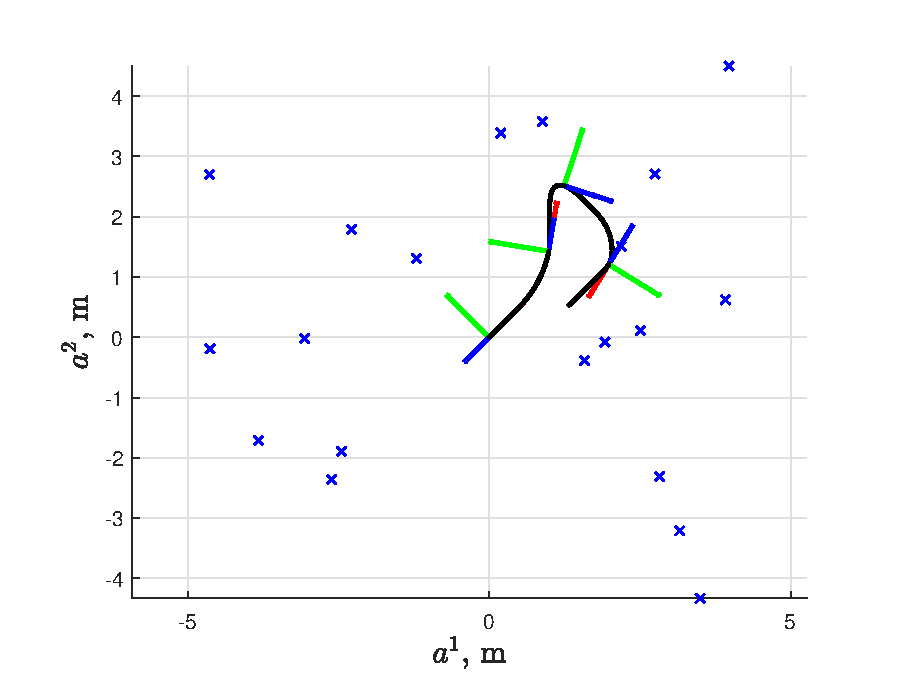
\includegraphics[width=\textwidth]{figs/batch/traj_xy.eps} 
        \end{subfigure}
        \hfill
        \begin{subfigure}[b]{0.495\textwidth}  
            \centering 
            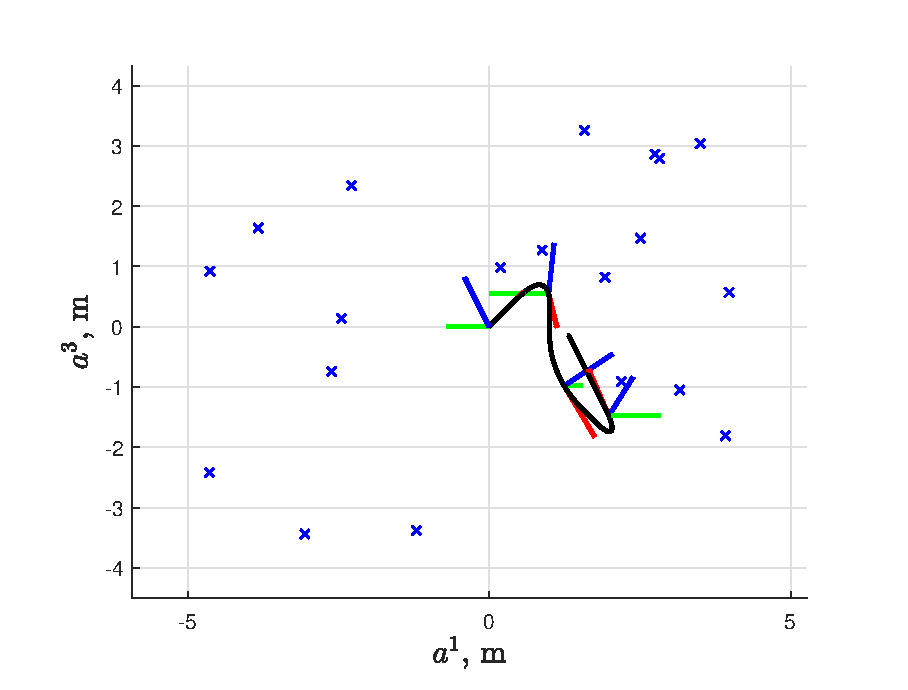
\includegraphics[width=\textwidth]{figs/batch/traj_xz.eps} 
        \end{subfigure}
        \vskip\baselineskip
        \begin{subfigure}[b]{0.495\textwidth}   
            \centering 
            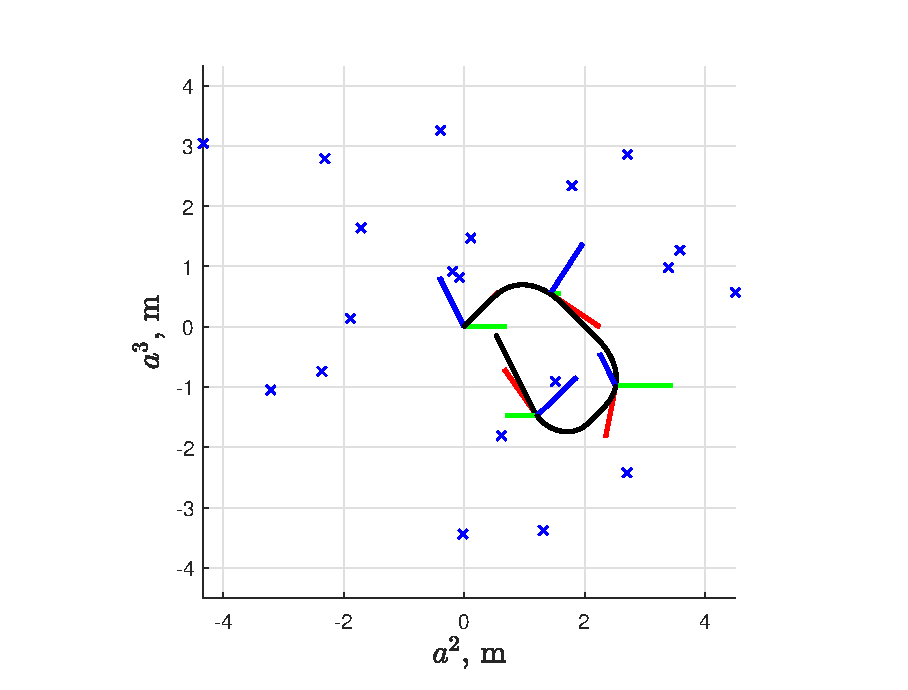
\includegraphics[width=\textwidth]{figs/batch/traj_yz.eps}  
        \end{subfigure}
        \hfill
        \begin{subfigure}[b]{0.495\textwidth}   
            \centering 
            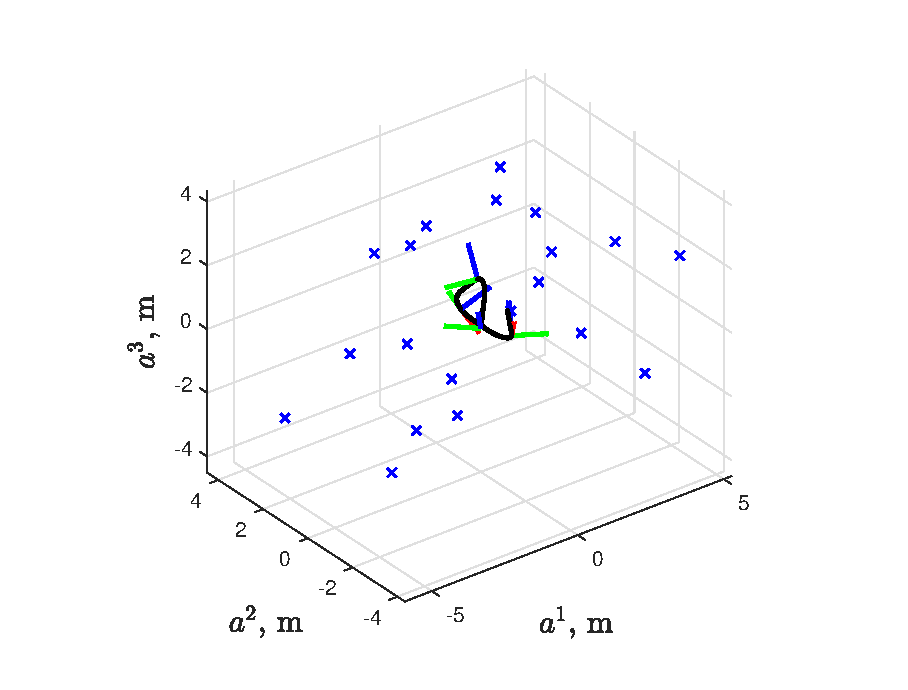
\includegraphics[width=\textwidth]{figs/batch/traj.eps} 
        \end{subfigure} 
	\caption[Trajectory used in simulations.]{Trajectory used in simulations. The blue markers represent the landmarks, the trajectory is shown in black, and a triad is used to show the orientation at various times during the trajectory.}
	\label{fig:batch_traj}
\end{figure}

\begin{table}[]
\centering
\begin{tabular}{|l|l|l|l|l|l|}
\hline
Trial                                            & $\sigma_k^1$ \si{\radian}          & $\sigma_k^2$ \si{m/s} & $\sigma_k^3$ \si{rad/s^2} & $\sigma_k^4$ \si{m/s^2} & $\sigma_{k,j}$ \si{m}      \\ \hhline{|=|=|=|=|=|=|}
\multicolumn{1}{|l|}{Rate Gyro Noise}            & \multicolumn{1}{l|}{0.05 to 1} & \multicolumn{1}{l|}{0.05}     & \multicolumn{1}{l|}{0.005} & \multicolumn{1}{l|}{0.005} & \multicolumn{1}{l|}{0.05}     \\ \hline
\multicolumn{1}{|l|}{Accelerometer Noise}  & \multicolumn{1}{l|}{0.05} & \multicolumn{1}{l|}{0.05 to 1}     & \multicolumn{1}{l|}{0.001} & \multicolumn{1}{l|}{0.005} & \multicolumn{1}{l|}{0.05}     \\ \hline
\multicolumn{1}{|l|}{Rate Gyro Bias Noise}  & \multicolumn{1}{l|}{0.05} & \multicolumn{1}{l|}{0.05}     & \multicolumn{1}{l|}{0 to 0.1} & \multicolumn{1}{l|}{0.005} & \multicolumn{1}{l|}{0.05}     \\ \hline
\multicolumn{1}{|l|}{Accelerometer Bias Noise} & \multicolumn{1}{l|}{0.05} & \multicolumn{1}{l|}{0.05}     & \multicolumn{1}{l|}{0.005} & \multicolumn{1}{l|}{0 to 0.1} & \multicolumn{1}{l|}{0.05}     \\ \hline
\multicolumn{1}{|l|}{Landmark Sensor Noise} & \multicolumn{1}{l|}{0.05} & \multicolumn{1}{l|}{0.05}     & \multicolumn{1}{l|}{0.005} & \multicolumn{1}{l|}{0.005} & \multicolumn{1}{l|}{0.05 to 1}     \\ \hline
\end{tabular}
\caption{Standard deviation of the noise injected into each measurement for each trial.}
\label{tab:se3_batch}
\end{table}

The results are presented in Figures~\ref{fig:batch_gyro}~to~\ref{fig:batch_landmark}. The main takeaway is that, generally, the six different approaches provide similar results. In particular, there is no discernible difference between using the invariant formulations of the measurement error (Approaches 4, 5, and 6) as opposed to their standard counterparts (Approaches 1, 2, and 3). The results from Approaches 1, 2, 4, and 5 are similar to such an extent that they are often indistinguishable when they are overlaid. Furthermore, the impact of reducing the state dependence of the Jacobians is unclear. After multiple iterations of the nonlinear least squares solver, the operating trajectory begins approaching the truth trajectory. Thus, assuming the solver converges to the optimal solution, the Jacobians become more and more accurate. The advantage of state-independent Jacobians is most notable in situations when the Jacobians are normally inaccurate, which isn't the case here. In addition, the error definitions used to derive the Jacobians in Approaches 3 and 6 simply shift the state dependence from $\mbf{F}_k^1$ to weighting matrix $\mbf{W}_{u,k}$. Some additional observations are as follows.

\begin{itemize}
	\item Increasing the magnitude of the standard deviation of the noise in the gyro had the largest impact on the results, as seen in Figure~\ref{fig:batch_gyro}. While Approaches 2 and 5 have a lower mean RMSE over a wide range of noise magnitudes, these formulations converge much slower than the other approaches. In the end, the left-invariant error definition using the type 1 Jacobians performed best when the noise level was increased.
	\item In general, a measurement-dependent Jacobian should be avoided when there is a lot of noise in the measurement, as it increases greatly the amount of steps needed to converge
	\item The right-invariant approaches show improved performance when there is significant noise in the landmark sensor and the accelerometer.
\end{itemize}

\begin{figure}
	\centering
	\begin{subfigure}[b]{0.5\textwidth}
		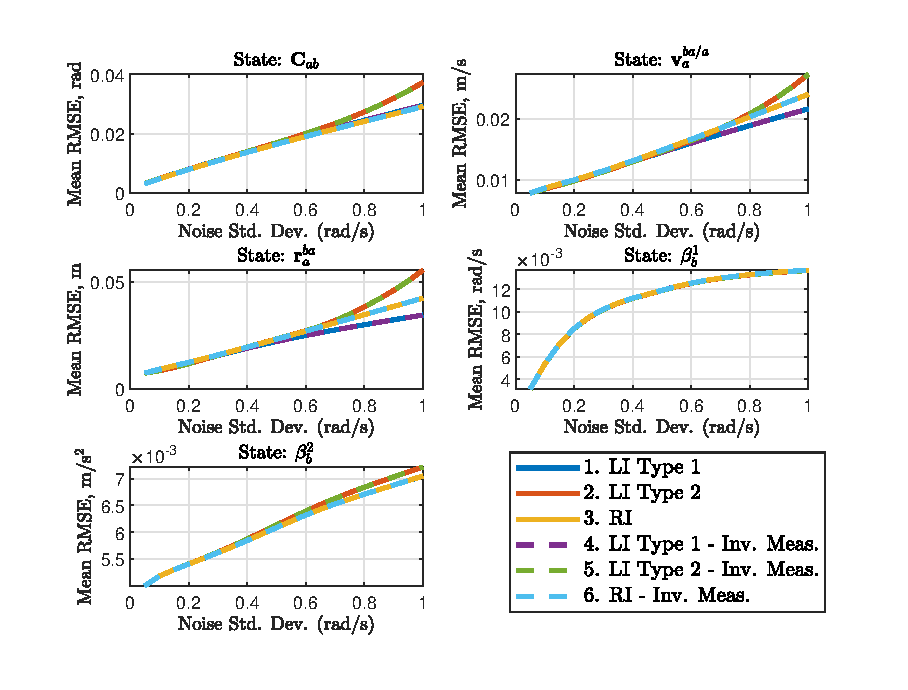
\includegraphics[width=\textwidth]{figs/batch/gyro_rmse.eps}
		\caption{Mean RMSE for each state.}
	\end{subfigure}
	~
	\begin{subfigure}[b]{0.5\textwidth}
		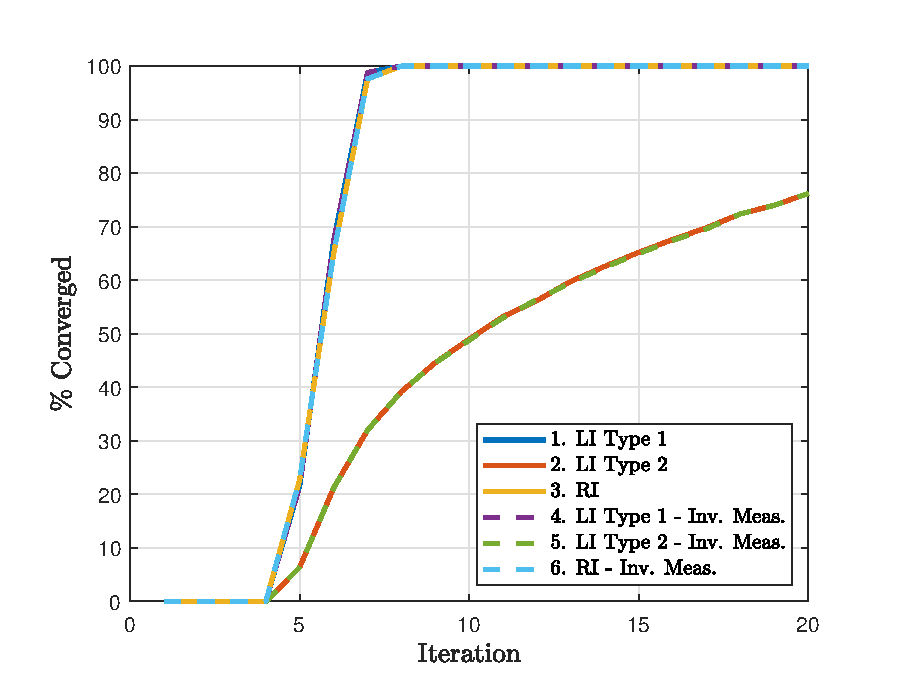
\includegraphics[width=\textwidth]{figs/batch/gyro_perc.eps}
		\caption{Percentage of trials that have converged at each GN iteration.}
	\end{subfigure}
	\caption[Results comparing batch SLAM approaches varying rate gyro noise.]{Results of 25 Monte Carlo trials comparing the various batch SLAM approaches, where the noise in the rate gyro was varied.}
	\label{fig:batch_gyro}
\end{figure}

\begin{figure}
	\centering
	\begin{subfigure}[b]{0.5\textwidth}
		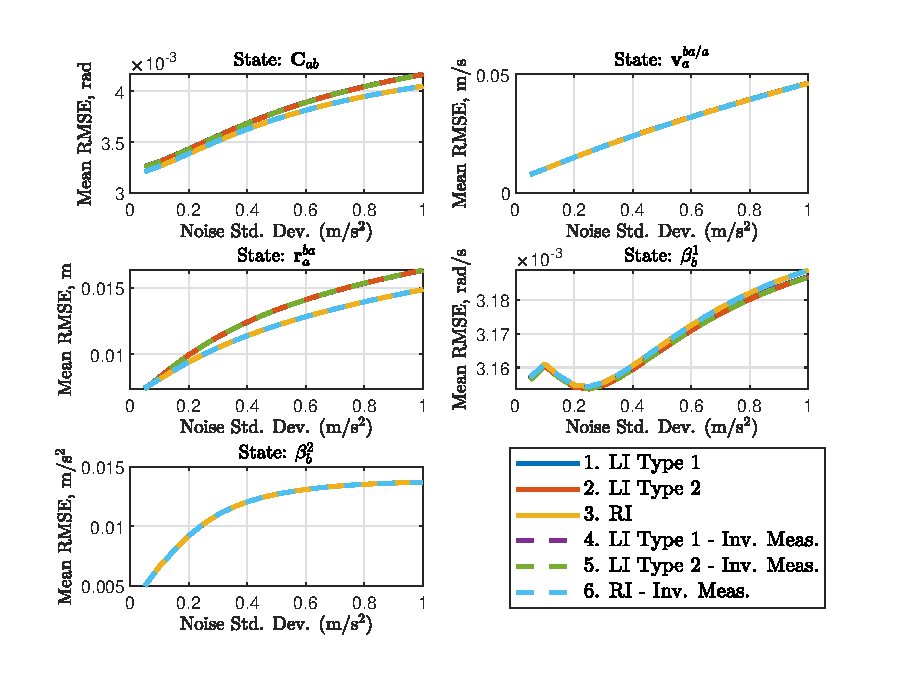
\includegraphics[width=\textwidth]{figs/batch/accel_rmse.eps}
		\caption{Mean RMSE for each state.}
	\end{subfigure}
	~
	\begin{subfigure}[b]{0.5\textwidth}
		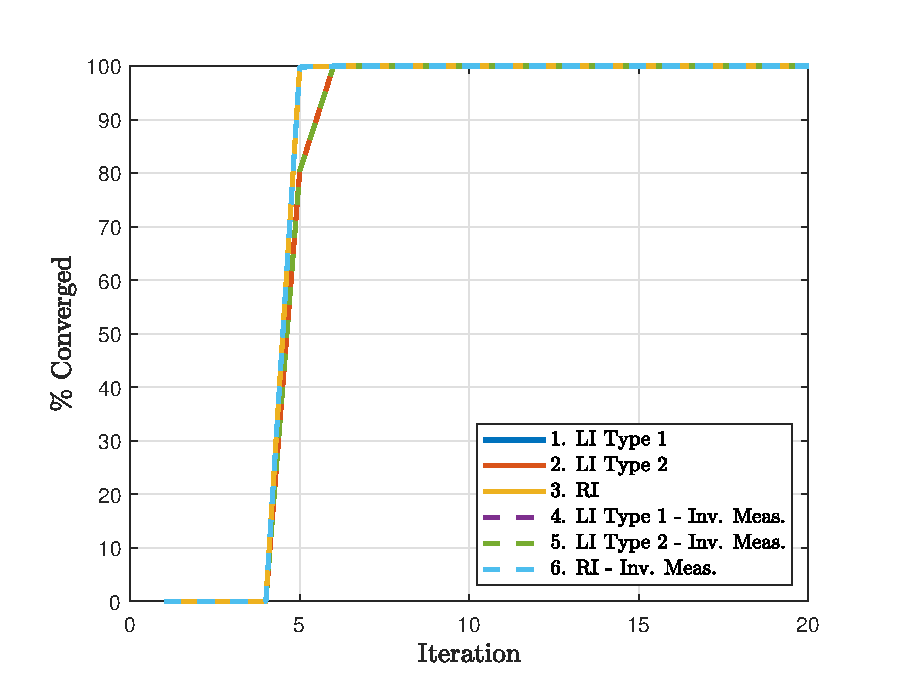
\includegraphics[width=\textwidth]{figs/batch/accel_perc.eps}
		\caption{Percentage of trials that have converged at each GN iteration.}
	\end{subfigure}
	\caption[Results comparing batch SLAM approaches varying zccelerometer noise.]{Results of 25 Monte Carlo trials comparing the various batch SLAM approaches, where the noise in the accelerometer was varied.}
	\label{fig:batch_accel}
\end{figure}  

\begin{figure}
	\centering
	\begin{subfigure}[b]{0.5\textwidth}
		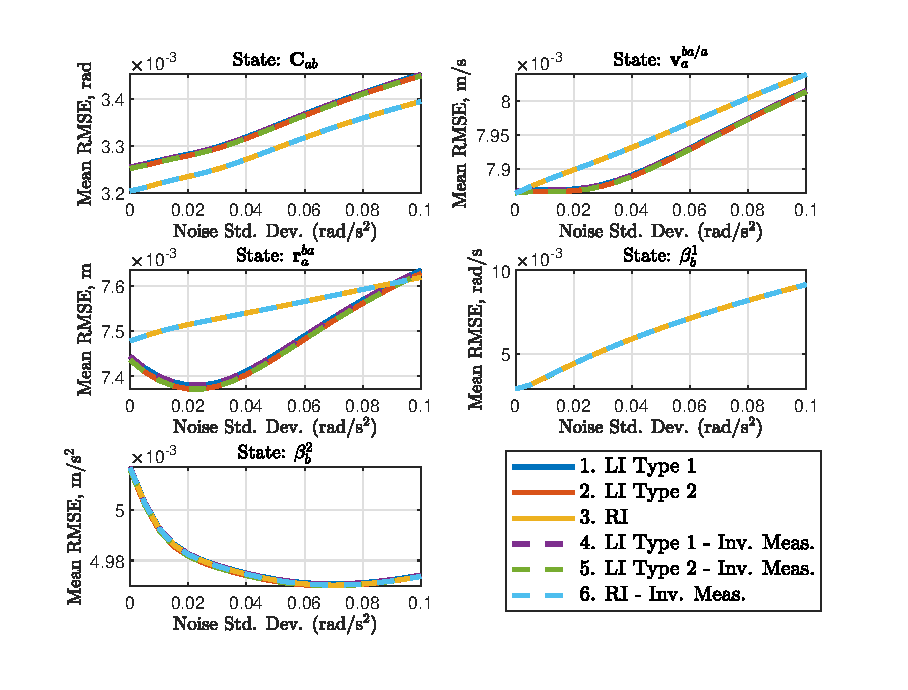
\includegraphics[width=\textwidth]{figs/batch/gyro_bias_rmse.eps}
		\caption{Mean RMSE for each state.}
	\end{subfigure}
	~
	\begin{subfigure}[b]{0.5\textwidth}
		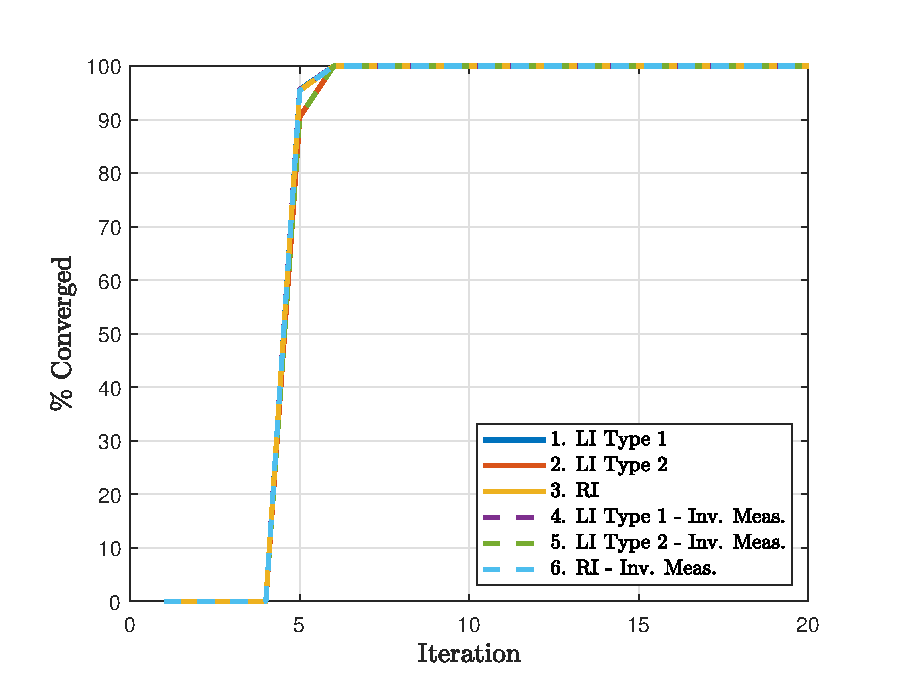
\includegraphics[width=\textwidth]{figs/batch/gyro_bias_perc.eps}
		\caption{Percentage of trials that have converged at each GN iteration.}
	\end{subfigure}
	\caption[Results comparing batch SLAM approaches vvarying rate gyro bias noise.]{Results of 25 Monte Carlo trials comparing the various batch SLAM approaches, where the noise in the gyro bias was varied.}
	\label{fig:batch_gyro_bias}
\end{figure} 


\begin{figure}
	\centering
	\begin{subfigure}[b]{0.5\textwidth}
		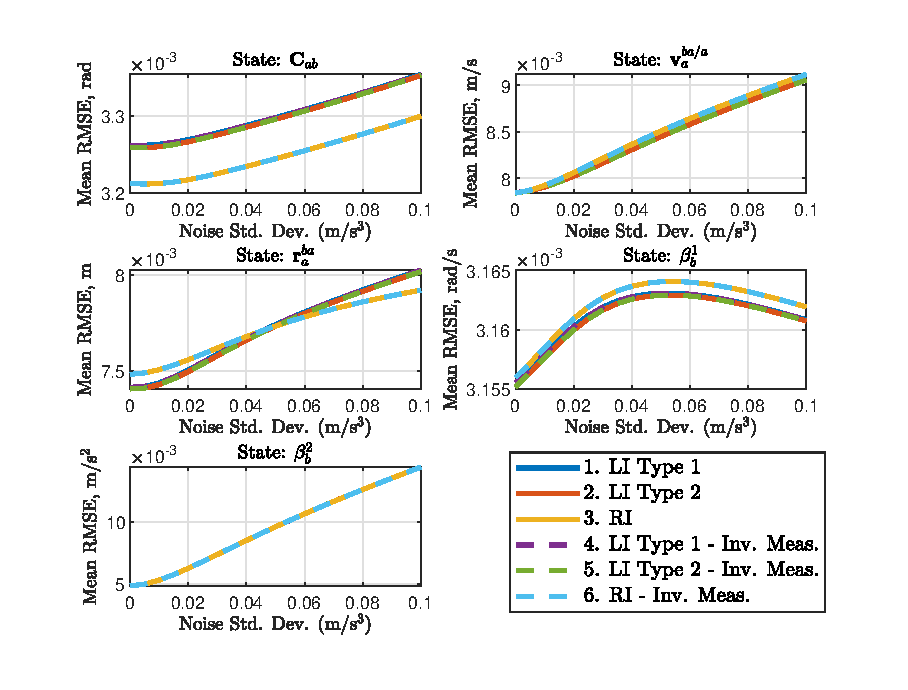
\includegraphics[width=\textwidth]{figs/batch/accel_bias_rmse.eps}
		\caption{Mean RMSE for each state.}
	\end{subfigure}
	~
	\begin{subfigure}[b]{0.5\textwidth}
		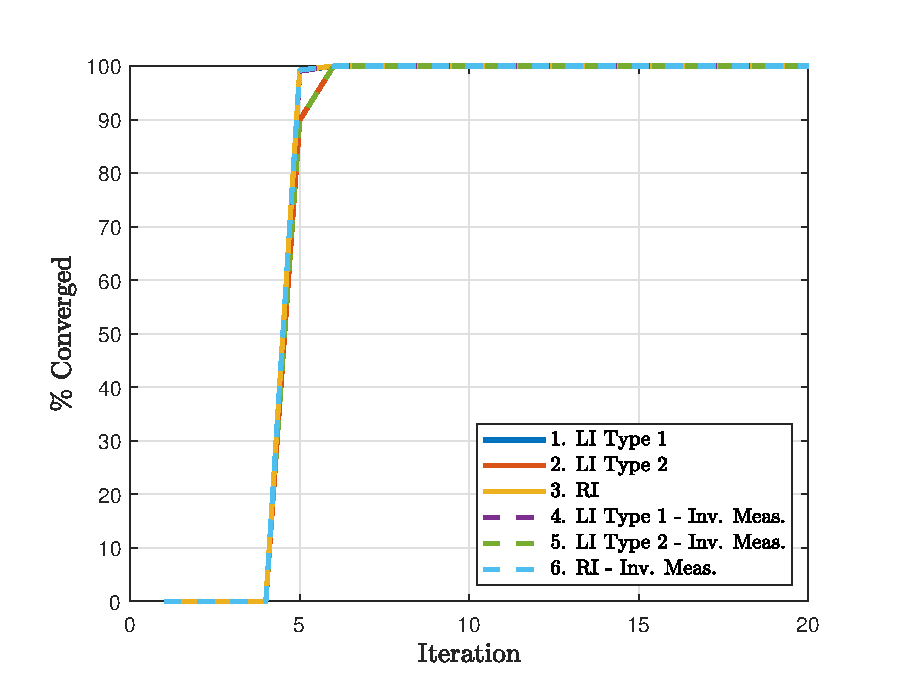
\includegraphics[width=\textwidth]{figs/batch/accel_bias_perc.eps}
		\caption{Percentage of trials that have converged at each GN iteration.}
	\end{subfigure}
	\caption[Results comparing batch SLAM approaches vvarying accelerometer bias noise.]{Results of 25 Monte Carlo trials comparing the various batch SLAM approaches, where the noise in the accelerometer bias was varied.}
	\label{fig:batch_accel_bias}
\end{figure} 

\begin{figure}
	\centering
	\begin{subfigure}[b]{0.5\textwidth}
		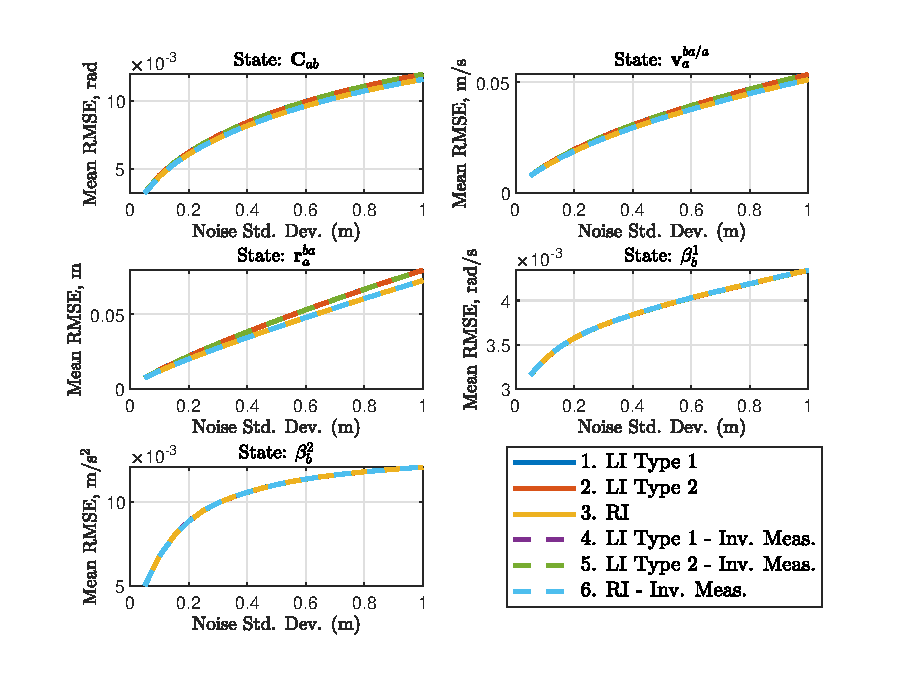
\includegraphics[width=\textwidth]{figs/batch/landmark_rmse.eps}
		\caption{Mean RMSE for each state.}
	\end{subfigure}
	~
	\begin{subfigure}[b]{0.5\textwidth}
		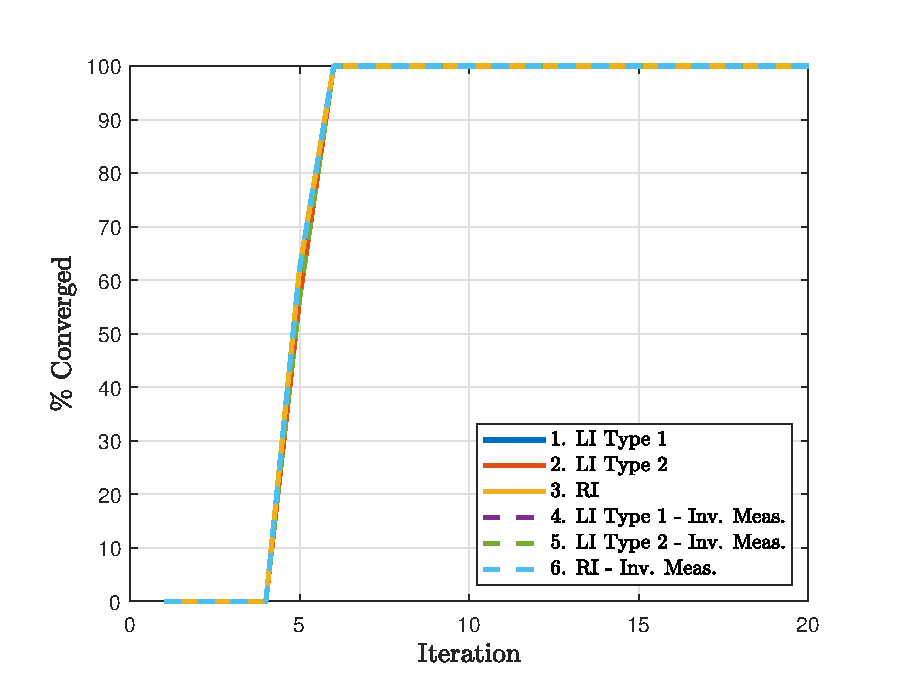
\includegraphics[width=\textwidth]{figs/batch/landmark_perc.eps}
		\caption{Percentage of trials that have converged at each GN iteration.}
	\end{subfigure}
	\caption[Results comparing batch SLAM approaches vvarying landmark sensor noise.]{Results of 25 Monte Carlo trials comparing the various batch SLAM approaches, where the noise in the landmark sensor was varied.}
	\label{fig:batch_landmark}
\end{figure}  

%  ------------------------------------------------------------
\cleardoublepage
  \chapter{Closing Remarks and Future Work}
  \label{chap:conc}
  \section{Conclusions}

In this thesis, an in-depth analysis of state estimation in an invariant framework is presented. Through rigorous testing, the advantages and limitations of these different techniques are determined. Furthermore, an extension of invariant filtering theory to the problem of a batch solution to the SLAM problem is presented.  

The IEKF is superior to the traditional MEKF in certain situations. It is better suited to problems where the state can be defined on matrix Lie groups, which is the case for many robotics problems. Throughout the simulations presented herein, the performance of the IEKF is on average better than that of the MEKF. However, only particular sample problems are used to illustrate this. It would therefore be irresponsible to state that the IEKF would always perform better than the MEKF. However, certain clear conclusions can be drawn.

First, state-independent Jacobians, such as those obtained in an IEKF, are advantageous in cases where the best estimate of the state is far from the true value. In most situations, this is seen when the initialization is poor. The IEKF's better performance is therefore mostly attributed to better performance in the transient period before the filter reaches steady state. Thus, the IEKF should be the state estimator of choice in applications where the initial state is unknown, and no other initialization scheme is available. 

Second, leveraging the invariant framework in batch estimation only has limited advantages. In standard batch estimation, the Jacobians may initially be inaccurate if they depend on the state. However, as the solution converges, the Jacobians will be closer to the true Jacobians, as the error in the state estimate decreases. At this stage, there is minimal difference between a state-independent Jacobian and a Jacobian computed using an accurate state estimate. 

\section{Future Work}

In Chapter~\ref{chap:SE3}, the IEKF is compared to the MEKF. The MEKF was used a baseline as it is commonly used. However, comparing the IEKF to an iterative version of the MEKF may yield different results. The iterative MEKF improves upon the MEKF by recomputing the Jacobians at each time step until convergence. Furthermore, an iterative version of the IEKF could also be developed. This iterative IEKF would only be useful in scenarios where the process model is not group affine, or the measurement model is not invariant, leading to state dependent Jacobians like the MEKF. 

Another avenue to explore would involve using a realistic sensor model in invariant batch SLAM. A future study using a stereo camera model or LIDAR model would also allow the invariant batch SLAM algorithms to be tested on experimental data.

Lastly, a study analyzing the consistency of the IEKF versus other other filtering techniques should be conducted. The IEKF should theoretically be more consistent, as its more accurate Jacobians mean the covariance better captures the underlying distribution. In a similar vein, the impact of unknown disturbances should be studied. The IEKF may be better suited to handle these, once again, due to theoretically exact Jacobians.
%  ------------------------------------------------------------

%   // Chapters
%%%%%%%%%%%%%%%%%%%%%%%%%%%%%%%%%%%%%%%%%%%%%%%%%%%%%%%%%%%%%%%%%%%%%%%%%%%%%%%%


% // Main matter
%%%%%%%%%%%%%%%%%%%%%%%%%%%%%%%%%%%%%%%%%%%%%%%%%%%%%%%%%%%%%%%%%%%%%%%%%%%%%%%%

%%%%%%%%%%%%%%%%%%%%%%%%%%%%%%%%%%%%%%%%%%%%%%%%%%%%%%%%%%%%%%%%%%%%%%%%%%%%%%%%
% End matter
\bookmarksetupnext{startatroot}

\cleardoublepage
% \startbibliography

% \pagestyle{bib}

 \begin{singlespace} % Bibliography must be single spaced
	% \bibliographystyle{ieeetr}
 	% \bibliography{refs}   % Use the BibTeX file ``References.bib''.
   \printbibliography
 \end{singlespace}

  % An external Abstract that can be printed at the end of the document,
  % for separate submission to Rackham. Comment it out when not needed. - jg
  % \startextabstractpage
  % {The Title of Your Dissertation}{Your Name}{Chair: Albert Einstein}
  % \input{Abstract/Abstract}
  % \label{ExtAbstract}

 % // End matter
%%%%%%%%%%%%%%%%%%%%%%%%%%%%%%%%%%%%%%%%%%%%%%%%%%%%%%%%%%%%%%%%%%%%%%%%%%%%%%%%
\end{document}